%%%%(c)
%%%%(c)  This file is a portion of the source for the textbook
%%%%(c)
%%%%(c)    Abstract Algebra: Theory and Applications
%%%%(c)    Copyright 1997 by Thomas W. Judson
%%%%(c)
%%%%(c)  See the file COPYING.txt for copying conditions
%%%%(c)
%%%%(c)
\documentclass[11pt]{book}
\usepackage{aatamacros} % lhm 2013/08/04 macros moved to style file
%
\aatamakeindex
%
\begin{document}
%
\frontmatter
%
\aatamaketitle
%
%%%%(c)
%%%%(c)  This file is a portion of the source for the textbook
%%%%(c)
%%%%(c)    Abstract Algebra: Theory and Applications
%%%%(c)    Copyright 1997 by Thomas W. Judson
%%%%(c)
%%%%(c)  See the file COPYING.txt for copying conditions
%%%%(c)
%%%%(c)
\chapter*{Preface}
 
% Print versions need a ToC entry
% tex4ht versions get their own ToC automatically
\ifthenelse{\boolean{basic}}{%
\phantomsection
\addcontentsline{toc}{chapter}{Preface}
\pagestyle{myheadings}
\markboth{PREFACE}{PREFACE}
}{}
 
 
 
 
This text is intended for a one- or two-semester undergraduate course
in  abstract algebra. Traditionally, these courses have covered the
theoretical aspects of groups, rings, and fields.  However, with the
development of computing in the last several decades, applications
that involve abstract algebra and discrete mathematics have become
increasingly important, and many science, engineering, and computer 
science students are now electing to minor in mathematics. Though
theory still occupies a central role in the subject of abstract
algebra and no student should go through such a course without a good
notion of what a proof is, the importance of applications such as
coding theory and cryptography has grown significantly.


Until recently most abstract algebra texts included few if any
applications. However, one of the major problems in teaching an
abstract algebra course is that for many students it is their first
encounter with an environment that requires them to do rigorous
proofs. Such students often find it hard to see the use of learning to
prove theorems and propositions; applied examples help the instructor
provide motivation. 
 
 

This text contains more material than can
possibly be covered in a single semester.  Certainly there is adequate
material for a two-semester course, and perhaps more; however, for a
one-semester course it would be quite easy to omit selected chapters
and still have a useful text.  The order of presentation of topics is
standard: groups, then rings, and finally fields. Emphasis can be
placed either on theory or on applications. A typical one-semester
course might cover groups and rings while briefly touching on field
theory, using Chapters~1 through 6, 9, 10, 11, 13 (the first part), 16, 17,
18 (the first part), 20, and 21. Parts of these chapters could be
deleted and applications substituted according to the interests of the
students and the instructor. A two-semester course emphasizing theory
might cover Chapters~1 through 6, 9, 10, 11, 13 through 18, 20, 21, 22 (the
first part), and 23. On the other hand, if applications are to be
emphasized, the course might cover Chapters 1 through 14, and 16
through 22. In an applied course, some of the more theoretical results
could be assumed or omitted. A chapter dependency chart appears below.
(A broken line indicates a partial dependency.)  



\begin{figure}[htb]


\begin{center}

\tikzpreface{dependencies}

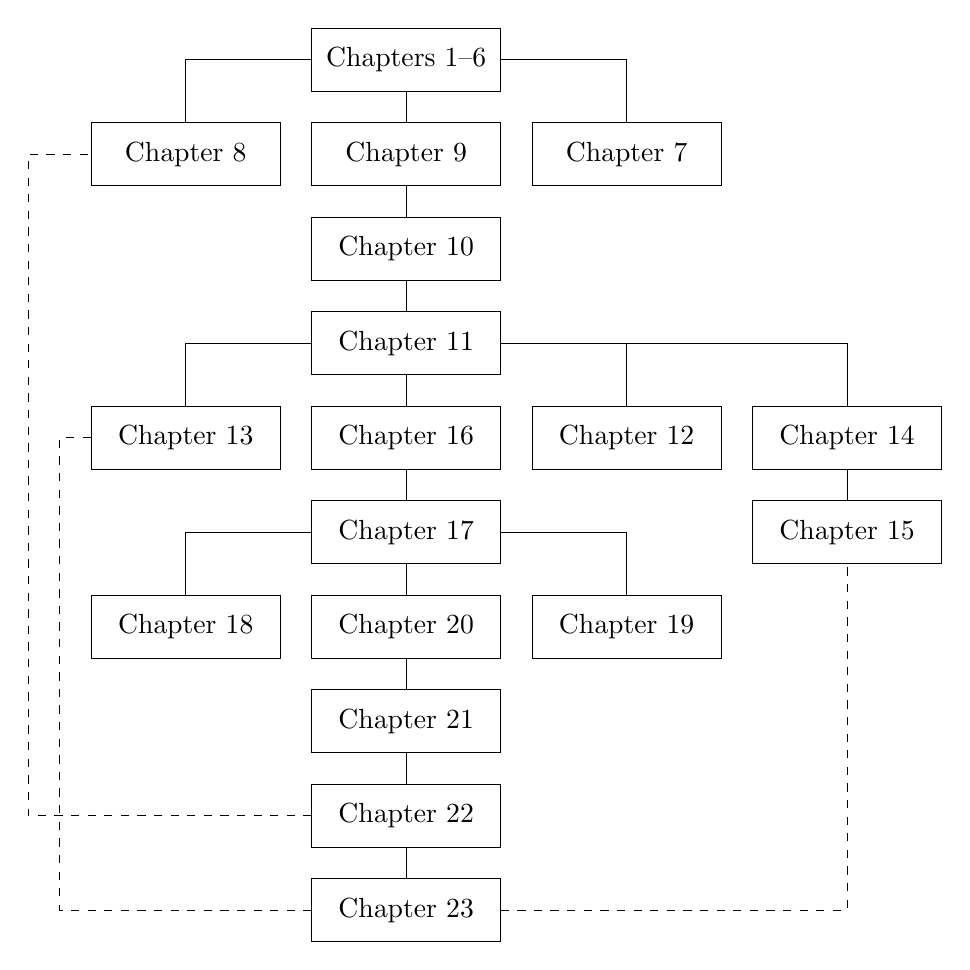
\begin{tikzpicture}[scale=0.8]  %Replaced figure with tikz figure - TWJ 6/14/2010

\draw (3.5,0) rectangle (6.5,1);
\node at (5,0.5) {Chapter 23};

\draw (3.5,1.5) rectangle (6.5,2.5);
\node at (5,2) {Chapter 22};

\draw (3.5,3) rectangle (6.5,4);
\node at (5,3.5) {Chapter 21};

\draw (0,4.5) rectangle (3,5.5);
\node at (1.5,5) {Chapter 18};

\draw (3.5,4.5) rectangle (6.5,5.5);
\node at (5,5) {Chapter 20};

\draw (7,4.5) rectangle (10,5.5);
\node at (8.5,5) {Chapter 19};

\draw (3.5,6) rectangle (6.5,7);
\node at (5,6.5) {Chapter 17};

\draw (10.5,6) rectangle (13.5,7);
\node at (12,6.5) {Chapter 15};

\draw (0,7.5) rectangle (3,8.5);
\node at (1.5,8) {Chapter 13};

\draw (3.5,7.5) rectangle (6.5,8.5);
\node at (5,8) {Chapter 16};

\draw (7,7.5) rectangle (10,8.5);
\node at (8.5,8) {Chapter 12};

\draw (10.5,7.5) rectangle (13.5,8.5);
\node at (12,8) {Chapter 14};

\draw (3.5,9) rectangle (6.5,10);
\node at (5,9.5) {Chapter 11};

\draw (3.5,10.5) rectangle (6.5,11.5);
\node at (5,11) {Chapter 10};

\draw (0,12) rectangle (3,13);
\node at (1.5,12.5) {Chapter 8};

\draw (3.5,12) rectangle (6.5,13);
\node at (5,12.5) {Chapter 9};

\draw (7,12) rectangle (10,13);
\node at (8.5,12.5) {Chapter 7};

\draw (3.5,13.5) rectangle (6.5,14.5);
\node at (5,14) {Chapters 1--6};

\draw (5,1) -- (5,1.5) (5,2.5) -- (5,3)  (5,4) -- (5,4.5)  (5,5.5) -- (5,6)  (5,7) -- (5,7.5)  (5,8.5) -- (5,9)  (5,10) -- (5,10.5)  (5,11.5) -- (5,12)  (5,13) -- (5,13.5);

\draw [dashed] (6.5,0.5) -- (12,0.5) -- (12,6);

\draw (12,7) -- (12,7.5) (12,8.5) -- (12,9.5) -- (6.5,9.5) (8.5,8.5) -- (8.5,9.5);

\draw (8.5,5.5) -- (8.5,6.5) -- (6.5,6.5);

\draw (8.5,13) -- (8.5,14) -- (6.5,14);

\draw [dashed] (3.5,0.5) -- (-0.5,0.5) -- (-0.5,8) -- (0,8);

\draw [dashed] (3.5,2) -- (-1,2) -- (-1,12.5) -- (0,12.5);

\draw (1.5,5.5) -- (1.5,6.5) -- (3.5,6.5);

\draw (1.5,8.5) -- (1.5,9.5) -- (3.5,9.5);

\draw (1.5,13) -- (1.5,14) -- (3.5,14);

\end{tikzpicture}

\end{center}
\end{figure}

Though there are no specific prerequisites for a course in abstract
algebra, students who have had other higher-level courses in
mathematics will generally be more prepared than those who have not,
because they will possess a bit more mathematical sophistication.
Occasionally, we shall assume some basic linear algebra; that is, we
shall take for granted an elementary knowledge of matrices and
determinants. This should present no great problem, since most
students taking a course in abstract algebra have been introduced to
matrices and determinants elsewhere in their career, if they have not
already taken a sophomore- or junior-level course in linear algebra.

Exercise sections are the heart of any mathematics text. An exercise
set appears at the end of each chapter. The nature of the exercises
ranges over several categories; computational,  conceptual, and
theoretical problems are included. A section presenting hints and
solutions to many of the exercises appears at the end of the text.
Often in the solutions a proof is only sketched, and it is up to the
student to provide the details. The exercises range in difficulty from
very easy to very challenging. Many of the more substantial problems
require careful thought, so the student should not be discouraged if
the solution is not forthcoming after a few minutes of work. 
% A complete solutions manual is available for the instructor's use. 
% Removed reference to the solutions manual.  TWJ 8/19/2010

There are additional exercises or computer projects at the ends of
many of the chapters. The computer projects usually require a
knowledge of programming. All of these exercises and projects are more
substantial in nature and allow the exploration of new results and
theory.

% Added Sage blurb, RAB 2011/07/28
Sage (\url{sagemath.org}) is a free, open source, software system
for advanced mathematics, which is ideal for assisting with a study
of abstract algebra. Comprehensive discussion about Sage, and a
selection of relevant exercises, are provided in an electronic
format that may be used with the Sage Notebook in a web browser,
either on your own computer, or at a public server such as
\url{sagenb.org}.  Look for this supplement at the book's
website: \url{abstract.pugetsound.edu}.  In printed
versions of the book, we include a brief description of Sage's
capabilities at the end of each chapter, right after the references.

The open source version of this book has received support from the National Science Foundation (Award \# 1020957).
%Added NSF support statement.  TWJ 8/9/2012

\section*{Acknowledgements}

I would like to acknowledge the following reviewers for their helpful
comments and suggestions. 
\begin{itemize}
 
\item
David Anderson,
University of Tennessee, Knoxville

\item
Robert Beezer,
University of Puget Sound

\item
Myron Hood,
California Polytechnic State University

\item
Herbert Kasube,
Bradley University

\item
John Kurtzke,
University of Portland
 
\item
Inessa Levi,
University of Louisville
 
\item
Geoffrey Mason,
University of California, Santa Cruz

\item
Bruce Mericle,
Mankato State University
 
\item
Kimmo Rosenthal,
Union College

\item
Mark Teply,
University of Wisconsin

\end{itemize}
I would also like to thank Steve Quigley, Marnie Pommett, Cathie
Griffin, Kelle Karshick, and the rest of the staff at PWS for their
guidance throughout this project. It has been a pleasure to work with
them. 

 
\begin{flushright}
Thomas W. Judson
\end{flushright}
 
 
\pagestyle{headings}
 
 
 
 

%
\aatatableofcontents
%
\mainmatter
%
%% TWJ, 2010/03/31
%% Chapters now begin with Chapter 1
%% \setcounter{chapter}{-1}
%
%%%%(c)
%%%%(c)  This file is a portion of the source for the textbook
%%%%(c)
%%%%(c)    Abstract Algebra: Theory and Applications
%%%%(c)    by Thomas W. Judson
%%%%(c)
%%%%(c)    Sage Material
%%%%(c)    Copyright 2011 by Robert A. Beezer
%%%%(c)
%%%%(c)  See the file COPYING.txt for copying conditions
%%%%(c)
%%%%(c)
\begin{sageverbatim}\end{sageverbatim}
%
\sageexercise{1}%
This exercise is just about making sure you know how to use Sage.  Login to a notebook server and create a new worksheet.  Do some non-trivial computation, maybe a pretty plot or some gruesome numerical computation to an insane precision.   Create an interesting list and experiment with it some.  Maybe include some nicely formatted text or \TeX\ using the included mini-word-processor (hover until a blue bar appears between cells and then shift-click).\par
%
Use whatever mechanism your instructor has in place for submitting your work.  Or save your worksheet and then trade worksheets via email (or another electronic method) with a classmate.
\begin{sageverbatim}\end{sageverbatim}
%
     %Set Theory
%%%%(c)
%%%%(c)  This file is a portion of the source for the textbook
%%%%(c)
%%%%(c)    Abstract Algebra: Theory and Applications
%%%%(c)    Copyright 1997 by Thomas W. Judson
%%%%(c)
%%%%(c)  See the file COPYING.txt for copying conditions
%%%%(c)
%%%%(c)
\chap{The Integers}{integers}


 
 
The integers are the building blocks of mathematics. In this chapter we will investigate  the fundamental properties of the integers, including mathematical induction, the division algorithm, and the Fundamental Theorem of Arithmetic.


\section{Mathematical Induction}\label{integers:math_induction}

Suppose we wish to show that
\[
1 + 2 + \cdots + n = \frac{n(n + 1)}{2}
\]
for any natural number $n$. This formula is easily  verified for small numbers such as $n = 1$, 2, 3, or 4, but it is impossible to verify for all natural numbers on a case-by-case basis.  To prove the formula true in general, a more generic method is required.

Suppose we have verified the equation for the first $n$ cases.  We will attempt to show that we can generate the formula for the $(n + 1)$th case from this knowledge.  The formula is true for $n = 1$ since 
\[
1 = \frac{1(1 + 1)}{2}.
\]
If we have verified the first $n$ cases, then
\begin{align*}
1 + 2 + \cdots + n + (n + 1) & = \frac{n(n + 1)}{2} + n + 1 \\
& = \frac{n^2 + 3n + 2}{2} \\
& = \frac{(n + 1)[(n + 1) + 1]}{2}.
\end{align*}
This is exactly the formula for the $(n + 1)$th case.
 
This method of proof is known as \boldemph{mathematical induction}.  Instead of attempting to verify a statement about some subset $S$ of the positive integers ${\mathbb N}$ on a case-by-case basis, an impossible task if $S$ is an infinite set, we give a specific proof for the smallest integer being considered, followed by a generic argument showing that if the statement holds for a given case, then it must also hold for the next  case in the sequence.  We summarize mathematical induction in the following axiom. 

\medskip

\noindent
{\bf First Principle of Mathematical Induction.}\index{Induction!first principle of} 
Let $S(n)$ be a statement about integers for  $n \in {\mathbb N}$ and suppose $S(n_0)$ is true for some integer $n_0$.  If for all integers $k$ with $k \geq n_0$ $S(k)$ implies that $S(k+1)$ is true, then $S(n)$ is true for all integers $n$ greater than or equal to $n_0$.  

%wording change.  Suggested by P. Diethelm.  TWJ 22/4/2013

\begin{example}{induction_greater_than}
For all integers $n \geq 3$, $2^n > n + 4$. Since
\[
8 = 2^3 > 3 + 4 = 7,
\]
the statement is true for $n_0 = 3$.  Assume that $2^k > k + 4$ for $k \geq 3$.  Then $2^{k + 1} = 2 \cdot 2^{k} > 2(k + 4)$.  But 
\[
2(k + 4) = 2k + 8 > k + 5 = (k + 1) + 4
\]
since $k$ is positive.  Hence, by induction, the statement holds for all integers $n \geq 3$. 
\end{example}

\begin{example}{induction_divisible}
Every integer $10^{n + 1} + 3 \cdot 10^n + 5$ is divisible by 9 for $n \in {\mathbb N}$.  For $n = 1$, 
\[
10^{1 + 1} + 3 \cdot 10 + 5 = 135 = 9 \cdot 15
\]
is divisible by 9.  Suppose that $10^{k + 1} + 3 \cdot 10^k + 5$ is divisible by 9 for $k \geq 1$.  Then 
\begin{align*}
10^{(k + 1) + 1} + 3 \cdot 10^{k + 1} + 5
& =
10^{k + 2} + 3 \cdot 10^{k + 1} + 50 - 45 \\
& =
10 (10^{k + 1} + 3 \cdot 10^{k} + 5) - 45
\end{align*}
is divisible by 9.
\end{example}

\begin{example}{binomial_theorem}
We will prove the binomial theorem using mathematical induction; that is, 
\[
(a + b)^n = \sum_{k = 0}^{n} \binom{n}{k} a^k b^{n - k},
\]
where $a$ and $b$ are real numbers, $n \in \mathbb{N}$, and
\[
\binom{n}{k}
= \frac{n!}{k! (n - k)!}\label{factorial}
\]
is the binomial coefficient.\label{binomial}  We first show that
\[
\binom{n + 1}{k}
=
\binom{n}{k} + \binom{n}{k - 1}.
\]
This result follows from
\begin{align*}
\binom{n}{k} + \binom{n}{k - 1}
& =
\frac{n!}{k!(n - k)!}
+\frac{n!}{(k-1)!(n - k + 1)!} \\
& =
\frac{(n + 1)!}{k!(n + 1 - k)!} \\
& =
\binom{n + 1}{k}.
\end{align*}
If $n = 1$, the binomial theorem is easy to verify. Now assume that the result is true for $n$ greater than or equal to 1.  Then
\begin{align*}
(a + b)^{n + 1}
& = 
(a + b)(a + b)^n \\
& =
(a + b) 
\left(
\sum_{k = 0}^{n} \binom{n}{k} a^k b^{n - k}
\right) \\
& = 
\sum_{k = 0}^{n} \binom{n}{k} a^{k + 1} b^{n - k}   +
\sum_{k = 0}^{n} \binom{n}{k} a^k b^{n + 1 - k} \\
& = 
a^{n + 1} + \sum_{k = 1}^{n} \binom{n}{k - 1} a^{k} b^{n + 1 - k} 
 +
\sum_{k = 1}^{n} \binom{n}{k}  a^k b^{n + 1 - k} + b^{n + 1}\\
&  = 
a^{n + 1} + \sum_{k = 1}^{n} \left[ \binom{n}{k - 1}
+
\binom{n}{k} \right]
a^k b^{n + 1 - k} + b^{n + 1} \\
&  = 
\sum_{k = 0}^{n + 1}   \binom{n + 1}{k} a^k b^{n + 1- k}.
\end{align*}
\end{example}
 
We have an equivalent statement of the Principle of Mathematical Induction that is often very useful.
 
\medskip

\noindent 
{\bf Second Principle of Mathematical Induction.}\index{Induction!second principle of}  
Let $S(n)$ be a statement about integers for  $n \in {\mathbb N}$ and suppose $S(n_0)$ is true for some integer $n_0$.  If $S(n_0), S(n_0 + 1), \ldots, S(k)$ imply that $S(k + 1)$ for $k \geq n_0$, then the statement $S(n)$ is true for all integers $n \geq n_0$.   

%wording change.  Suggested by P. Diethelm.  TWJ 22/4/2013
 
\medskip

A  nonempty subset $S$ of ${\mathbb Z}$ is \boldemph{well-ordered\/}\index{Well-ordered set} if $S$ contains a least element.  Notice that the set ${\mathbb Z}$ is not well-ordered since it does not contain a smallest element.  However, the natural numbers are well-ordered. 
 
\medskip
 
\noindent {\bf Principle of Well-Ordering.} 
Every nonempty subset of the natural numbers is well-ordered. 

\medskip
 
The Principle of Well-Ordering is equivalent to the Principle  of Mathematical Induction. 
 
\begin{lemma}\label{integers:smallest_number_lemma}
The Principle of Mathematical Induction implies that $1$ is the least positive natural number. 
\end{lemma}

\begin{proof}
Let $S = \{ n \in {\mathbb N} : n \geq 1 \}$. Then $1 \in S$.  Now assume that $n \in S$; that is, $n \geq 1$.  Since $n+1 \geq 1$, $n+ 1 \in S$; hence, by induction, every natural number is greater than or equal to 1. 
\end{proof}

% Theorem reworded for clarity.  TWJ 12/17/2011
% Suggested by K. Halasz and R. Beezer.
\begin{theorem}\label{integers_PMI_implies_PWO}
The Principle of Mathematical Induction implies the Principle of Well-Ordering.  That is, every nonempty subset of $\mathbb N$ contains a least element.
\end{theorem}
 
\begin{proof}
We must show that if $S$ is a nonempty subset of the natural numbers, then $S$ contains a least element.  If $S$ contains 1, then the theorem is true by Lemma~\ref{integers:smallest_number_lemma}.  Assume that if $S$ contains an integer $k$ such that $1 \leq k \leq n$, then $S$ contains a least element.  We will show that if a set $S$ contains an integer less than or equal to $n + 1$, then $S$ has a least element.  If $S$ does not contain an integer less than $n+1$, then $n+1$ is the smallest integer in $S$.  Otherwise, since $S$ is nonempty, $S$ must contain an integer less than or equal to $n$. In this case, by induction, $S$ contains a least element. 
\hspace*{1in} 
\end{proof}

%wording change.  Suggested by P. Diethelm.  TWJ 22/4/2013
 
\medskip
 
Induction can also be very useful in formulating definitions.  For instance, there are two ways to define $n!$, the factorial of a positive integer $n$. 
\begin{itemize}
 
\item 
The \emph{explicit} definition: $n! = 1 \cdot 2 \cdot 3 \cdots (n - 1)
\cdot n$. 
 
\item 
The \emph{inductive} or \emph{recursive} definition: $1! = 1$ and
$n! = n(n - 1)!$ for $n > 1$. 
 
\end{itemize}
Every good mathematician or computer scientist knows that looking at problems recursively, as opposed to explicitly, often results in better understanding of complex issues.  

 
\section{The Division Algorithm}

An application of the Principle of Well-Ordering that we will use often is the division algorithm. 

\begin{theorem}[Division Algorithm]\label{integers:division_algorithm}\index{Division algorithm!for integers}
Let $a$ and $b$ be integers, with $b > 0$.  Then there exist unique integers $q$ and $r$ such that 
\[
a = bq + r
\]
where $0 \leq r < b$.
\end{theorem}

\begin{proof}
This is a perfect example of the existence-and-uniqueness type of proof.  We must first prove that the numbers $q$ and $r$ actually  exist. Then we must show that if  $q'$ and $r'$ are two other such numbers, then $q = q'$ and $r = r'$. 
 
\emph{Existence of q and r}.
Let
\[
S = \{ a - bk : k \in {\mathbb Z} \text{ and } a - bk \geq 0 \}.
\]
If $0 \in S$, then $b$ divides $a$, and  we can let $q = a/b$ and $r = 0$.  If $0 \notin S$, we can use the Well-Ordering Principle.  We must first show that $S$ is nonempty.  If $a > 0$, then $a - b \cdot 0 \in S$. If $a < 0$, then $a - b(2a) = a(1 - 2b) \in S$.  In either case $S \neq \emptyset$.  By the Well-Ordering Principle, $S$ must have a smallest member, say $r = a - bq$. Therefore, $a = bq + r$, $r \geq 0$. We now show that $r < b$. Suppose that $r > b$. Then   
\[
a - b(q + 1)= a - bq - b = r - b > 0.
\]
In this case we would have $a - b(q + 1)$ in the set $S$. But then $a - b(q + 1) < a - bq$, which would contradict the fact that $r = a - bq$ is the smallest member  of $S$. So $r \leq b$.  Since $0 \notin S$, $r \neq b$ and so $r < b$. 
 
\emph{Uniqueness of q and r}.
Suppose there exist integers $r$, $r'$, $q$, and $q'$ such that
\[
a = bq + r, 0 \leq r < b 
\qquad
\text{and}
\qquad
a = bq' + r', 0 \leq r' < b.
\]
Then $ bq + r =  bq' + r'$.  Assume that $r' \geq r$.  From the last equation we have $b(q - q') = r' - r$; therefore, $b$ must divide $r' - r$ and $0 \leq r'- r \leq r' < b$.  This is possible only if $r' - r = 0$.  Hence, $r = r'$ and  $q = q'$. 
\end{proof}

\medskip

Let $a$ and $b$ be integers.  If $b = ak$ for some integer $k$, we write $a \mid b$\label{divides}.  An integer $d$ is called a \boldemph{common divisor} of $a$ and $b$ if $d \mid a$ and $d \mid b$.  The \boldemph{greatest common divisor}\index{Greatest common divisor!of two integers} of integers $a$ and $b$ is a positive integer $d$ such that $d$ is a common divisor  of $a$ and $b$ and if $d'$ is any other common divisor of $a$ and $b$, then $d' \mid d$.  We write $d = \gcd(a, b)$\label{greatestcd}; for example, $\gcd( 24, 36) = 12$ and $\gcd(120, 102) = 6$.  We say that two integers $a$ and $b$ are \boldemph{relatively prime} if $\gcd( a, b ) = 1$. 

\begin{theorem}\label{integers:gcd_theorem}
Let $a$ and $b$ be nonzero integers. Then there exist integers $r$ and $s$ such that
\[
\gcd( a, b) = ar + bs.
\]
Furthermore, the greatest common divisor of $a$ and $b$ is unique.
\end{theorem}
 
\begin{proof} %Notation error in proof fixed (pointed out by Rocco Rossi) - TWJ 9/13/2010
Let
\[
S = \{ am + bn : m, n \in {\mathbb Z} \text{ and } am + bn > 0 \}.
\]
Clearly, the set $S$ is nonempty; hence, by the Well-Ordering Principle $S$ must have a smallest member, say $d = ar + bs$.  We claim that $d = \gcd( a, b)$.  Write $a = dq + r'$ where $0 \leq r' < d$ . If $r' > 0$, then %r changed to r' - TWJ 1/31/2011
\begin{align*}
r '
& = a - dq \\
& = a - (ar + bs)q \\
& = a - arq - bsq \\
& = a( 1 - rq ) + b( -sq ),
\end{align*}
which is in $S$.  But this would contradict the fact that $d$ is the smallest member of $S$.  Hence, $r' = 0$ and $d$ divides $a$.  A similar argument shows that $d$ divides $b$.  Therefore, $d$ is a common divisor of $a$ and $b$.

Suppose that $d'$ is another common divisor of $a$ and $b$, and we want to show that $d' \mid d$. If we let $a = d'h$ and $b = d'k$, then
\[
d = ar + bs = d'hr + d'ks = d'(hr + ks).
\]
So $d'$ must divide $d$. Hence, $d$ must be the unique greatest common divisor of $a$ and $b$. 
\end{proof}

\begin{corollary}\label{integers:coprime_corollary}
Let $a$ and $b$ be two integers that are relatively prime. Then there exist  integers $r$ and $s$ such that $ar + bs = 1$. 
\end{corollary}
 
 
\subsection*{The Euclidean Algorithm}

Among other things, Theorem~\ref{integers:gcd_theorem} allows us to compute the greatest common divisor of two integers. 

\medskip

\begin{example}{gcd}
Let us compute the greatest common divisor of $945$ and $2415$.  First observe that 
\begin{align*}
2415 & = 945 \cdot 2 + 525 \\
945 & = 525 \cdot 1 + 420 \\
525 & = 420 \cdot 1 + 105 \\
420 & = 105 \cdot 4 + 0.
\end{align*}
Reversing our steps, 105 divides 420, 105 divides 525, 105 divides 945, and 105 divides 2415.  Hence, 105 divides both 945 and 2415.  If $d$ were another common divisor of 945 and 2415, then $d$ would also have to divide 105.  Therefore, $\gcd( 945, 2415 ) = 105$.

If we work backward through the above sequence of equations, we can also obtain numbers $r$ and $s$ such that $945 r + 2415 s = 105$.  Observe that 
\begin{align*}
105 & = 525 + (-1) \cdot 420 \\
& = 525 + (-1) \cdot [945 + (-1) \cdot 525] \\
& = 2 \cdot 525 + (-1) \cdot 945 \\
& = 2 \cdot [2415 + (-2) \cdot 945] + (-1) \cdot 945 \\
& = 2 \cdot 2415 + (-5) \cdot 945.
\end{align*}
So $r = -5$ and $s= 2$.  Notice that $r$ and $s$ are not unique, since $r = 41$ and $s = -16$ would also work.
\end{example}

To compute $\gcd(a,b) = d$, we are using repeated divisions to obtain a decreasing sequence of positive integers $r_1 > r_2 > \cdots > r_n = d$; that is,
\begin{align*}
b & = a q_1 + r_1 \\
a & = r_1 q_2 + r_2 \\
r_1 & = r_2 q_3 + r_3 \\
& \vdots  \\
r_{n - 2} & = r_{n - 1} q_{n} + r_{n} \\
r_{n - 1} & = r_n q_{n + 1}.
\end{align*}
To find $r$ and $s$ such that $ar + bs = d$, we begin with this last equation and substitute results obtained from the previous equations:
\begin{align*}
d & = r_n \\
& = r_{n - 2} - r_{n - 1} q_n \\
& = r_{n - 2} - q_n( r_{n - 3} - q_{n - 1} r_{n - 2} ) \\
& = -q_n r_{n - 3} + ( 1+ q_n q_{n-1} ) r_{n - 2}  \\
& \vdots  \\
& = ra + sb.
\end{align*}
The algorithm that we have just used to find the greatest common divisor $d$ of two integers $a$ and $b$ and to write $d$ as the linear combination of $a$ and $b$ is known as the \boldemph{Euclidean algorithm}\index{Euclidean algorithm}\index{Algorithm!Euclidean}.  
 
 
\subsection*{Prime Numbers}

Let $p$ be an integer such that $p > 1$.  We say that $p$ is a \boldemph{prime number}\index{Prime integer}, or simply $p$ is \boldemph{prime}, if the only positive numbers that divide $p$ are 1 and $p$ itself.  An integer $n > 1$ that is not prime is said to be \boldemph{composite}\index{Composite integer}.  

\begin{lemma}[Euclid]\label{integers:prime_divisor_theorem}
Let $a$ and $b$ be integers and $p$ be a prime number.  If $p \mid ab$, then either $p \mid a$ or $p \mid b$. 
\end{lemma}

\begin{proof}
Suppose that $p$ does not divide $a$.  We must show that $p \mid b$. Since $\gcd( a, p ) = 1$, there exist integers $r$ and $s$ such that $ar + ps = 1$.  So 
\[
b = b(ar + ps) = (ab)r + p(bs).
\]
Since $p$ divides both $ab$ and itself, $p$ must divide $b = (ab)r + p(bs)$. 
\end{proof}

\begin{theorem}[Euclid]\label{integers_inifinite_primes}
There exist an infinite number of primes.
\end{theorem}

\begin{proof}
We will prove this theorem by contradiction.  Suppose that there are only a finite number of primes, say $p_1, p_2, \ldots, p_n$.  Let $P = p_1  p_2  \cdots  p_n + 1$.    Then $P$ must be divisible by some $p_i$ for $1 \leq i \leq n$. In this  case, $p_i$ must divide $P - p_1 p_2 \cdots p_n = 1$, which is a contradiction.  Hence, either $P$ is prime or there exists an additional prime number $p \neq p_i$ that divides $P$.
\end{proof}
%Error in proof fixed.  Suggested by R. Rossi.  TWJ 12/19/2011

\begin{theorem}[Fundamental Theorem of Arithmetic]\label{integers_theorem_FTA}\index{Fundamental Theorem!of Arithmetic}
Let $n$ be an integer such that $n > 1$.  Then
\[
n = p_1 p_2 \cdots p_k,
\]
where $p_1, \ldots, p_k$ are  primes (not necessarily distinct).  Furthermore, this factorization is unique; that is, if 
\[
n = q_1 q_2 \cdots q_l,
\]
then $k = l$ and the $q_i$'s are just the $p_i$'s rearranged.
\end{theorem}

\begin{proof}
\emph{Uniqueness}.
To show uniqueness we will use induction on $n$. The theorem is certainly true for $n = 2$ since in this case $n$ is prime.  Now assume that the result holds for all integers $m$ such that $1 \leq m < n$, and 
\[
n = p_1 p_2 \cdots p_k = q_1 q_2 \cdots q_l,
\]
where $p_1 \leq p_2 \leq \cdots \leq p_k$ and $q_1 \leq q_2 \leq \cdots \leq q_l$. By Lemma~\ref{integers:prime_divisor_theorem}, $p_1  \mid  q_i$ for some $i = 1, \ldots, l$ and $q_1  \mid  p_j$ for some $j = 1, \ldots, k$.  Since all of the $p_i$'s and $q_i$'s are prime, $p_1 = q_i$ and  $q_1 = p_j$. Hence, $p_1 = q_1$ since $p_1 \leq p_j = q_1 \leq q_i = p_1$.  By the induction hypothesis, 
\[
n' = p_2 \cdots p_k = q_2 \cdots q_l
\]
has a unique factorization.  Hence, $k=l$ and $q_i = p_i$ for $i = 1, \ldots, k$. 

\emph{Existence}.
To show existence, suppose that there is some integer that cannot be written as the product of primes.  Let $S$ be the set of all such numbers.  By the Principle of Well-Ordering, $S$ has a smallest number, say $a$.  If the only positive factors of $a$ are $a$ and 1, then $a$ is prime, which is a contradiction.  Hence, $a = a_1 a_2$ where $1 < a_1 < a$ and $1 < a_2 < a$.  Neither $a_1\in S$ nor $a_2 \in S$, since $a$ is the smallest element in $S$.  So 
\begin{align*}
a_1 & = p_1 \cdots p_r \\
a_2 & = q_1 \cdots q_s.
\end{align*}
Therefore,
\[
a = a_1 a_2 = p_1 \cdots p_r q_1 \cdots q_s.
\]
So $a \notin S$, which is a contradiction.
\end{proof}
 
\histhead

\noindent
\parbox{\textwidth}
{\small \histf
Prime numbers were first studied by the ancient Greeks.  Two important results from antiquity are Euclid's proof that an infinite number of primes exist and the Sieve of Eratosthenes, a method of computing all of the prime numbers less than a fixed positive integer $n$.  One problem in number theory is to find a function $f$ such that $f(n)$ is prime for each integer $n$. Pierre Fermat (1601?--1665) conjectured that $2^{2^n} + 1$ was prime for all $n$, but later it was shown by Leonhard Euler (1707--1783) that 
\[
2^{2^5} + 1 = \text{4,294,967,297}
\]
is a composite number. One of the many unproven conjectures about prime numbers is Goldbach's Conjecture.  In a letter to Euler in 1742, Christian Goldbach stated the conjecture that every even integer with the exception of 2 seemed to be the sum of two primes:  $4 = 2 + 2$, $6 = 3 + 3$, $8 =3 + 5$, $\ldots$.  Although the conjecture has been verified for the numbers up through 100 million, it has yet to be proven in general.  Since prime numbers play an important role in public key cryptography, there is currently a great deal of interest in determining whether or not a large number is prime.
\histbox
}


\markright{EXERCISES}
\section*{Exercises}
\exrule

{\small
 
\begin{enumerate}
 
\item
Prove that
\[
1^2 + 2^2 + \cdots + n^2 = \frac{n(n + 1)(2n + 1)}{6}
\]
for $n \in {\mathbb N}$.

\item
Prove that
\[
1^3 + 2^3 + \cdots + n^3 = \frac{n^2(n + 1)^2}{4}
\]
for $n \in {\mathbb N}$.

\item
Prove that $n! > 2^n$ for $n \geq 4$.

\item
Prove that
\[
x + 4x + 7x + \cdots + (3n-2)x = \frac{n(3n - 1)x}{2}
\]
for $n \in {\mathbb N}$.

\item
Prove that $10^{n + 1} + 10^n + 1$ is divisible by 3 for $n \in {\mathbb N}$.

\item
Prove that $4 \cdot 10^{2n} + 9 \cdot 10^{2n - 1} + 5$ is divisible by 99 for $n \in {\mathbb N}$.

\item
Show that
\[
\sqrt[n]{a_1 a_2 \cdots a_n} \leq \frac{1}{n} \sum_{k = 1}^{n} a_k.
\]

\item
Prove the Leibniz rule for $f^{(n)} (x)$, where $f^{(n)}$ is the $n$th derivative of $f$; that is, show that 
\[
(fg)^{(n)} (x) = \sum_{k=0}^{n} \binom{n}{k} f^{(k)}(x) g^{(n-k)} (x).
\]

\item
Use induction to prove that $1 + 2 + 2^2 + \cdots + 2^n = 2^{n + 1} - 1$ for $n \in {\mathbb N}$. 

\item 
Prove that
\[
\frac{1}{2}+ \frac{1}{6} + \cdots + \frac{1}{n(n + 1)} = \frac{n}{n + 1} 
\]
for $n \in {\mathbb N}$.

\item 
If $x$ is a nonnegative real number, then show that $(1 + x)^n - 1 \geq nx$ for $n = 0, 1, 2, \ldots$. 
 
\item
\textbf{Power Sets.} 
Let $X$ be a set.  Define the \boldemph{power set}\index{Power set} of $X$, denoted ${\mathcal P}(X)$\label{powerset}, to be the set of all subsets  of $X$.  For example,  
\[
{\mathcal P}( \{a, b\} ) = \{ \emptyset, \{a\}, \{b\}, \{a, b\} \}.
\]
For every positive integer $n$, show that a set with exactly $n$ elements has a power set with exactly $2^n$ elements.

\item
Prove that the two principles of mathematical induction stated in Section~\ref{integers:math_induction} are equivalent. 

\item
Show that the Principle of Well-Ordering for the natural numbers implies that 1 is the smallest natural number.  Use this result to show that the Principle of Well-Ordering implies the Principle of Mathematical Induction; that is, show that if $S \subset {\mathbb N}$ such that $1 \in S$ and $n + 1 \in S$ whenever $n \in S$, then $S = {\mathbb N}$.  

\item
For each of the following pairs of numbers $a$ and $b$, calculate $\gcd(a,b)$ and find integers $r$ and $s$ such that  $\gcd(a,b) = ra + sb$. 
\begin{multicols}{2}
\begin{enumerate}

\item 
14 and 39

\item
234 and 165

\item
1739 and 9923

\item
471 and 562

\item
23,771 and 19,945

\item
$-4357$ and 3754

\end{enumerate}
\end{multicols}
 
\item 
Let $a$ and $b$ be nonzero integers. If there exist integers $r$ and $s$ such that $ar +bs =1$, show that $a$ and $b$ are relatively prime. 
 
 
\item
\textbf{Fibonacci Numbers.}
The Fibonacci numbers are
\[
1, 1, 2, 3, 5, 8, 13, 21, \ldots.
\]
We can define them inductively by $f_1 = 1$, $f_2 = 1$, and $f_{n + 2} = f_{n + 1} + f_n$ for $n \in {\mathbb N}$. 
\begin{enumerate}
 
 \item
Prove that $f_n < 2^n$.
 
 \item
Prove that $f_{n + 1} f_{n - 1} = f^2_n + (-1)^n$, $n \geq 2$.
 
 \item
Prove that $f_n = [(1 + \sqrt{5}\, )^n - (1 - \sqrt{5}\, )^n]/ 2^n \sqrt{5}$.
 
 \item
Show that $\lim_{n \rightarrow \infty} f_n / f_{n + 1} = (\sqrt{5} - 1)/2$. 
 
 \item
Prove that $f_n$ and $f_{n + 1}$ are relatively prime.
 
\end{enumerate}

\item
Let $a$ and $b$ be integers such that $\gcd(a,b) = 1$.  Let $r$ and $s$ be integers such that $ar + bs =1$.  Prove that 
\[
\gcd(a,s) = \gcd(r,b) = \gcd(r,s) =  1.
\]

\item
Let $x, y \in {\mathbb N}$ be relatively prime.  If $xy$ is a perfect square, prove that $x$ and $y$ must both be perfect squares.

\item
Using the division algorithm, show that every perfect square is of the form $4k$ or $4k + 1$ for some nonnegative integer $k$.

\item
Suppose that $a, b, r, s$ are pairwise relatively prime and that
\begin{align*}
a^2 + b^2 & = r^2 \\
a^2 - b^2 & = s^2.
\end{align*}
Prove that $a$, $r$, and $s$ are odd and $b$ is even.

%% TWJ 9/15/2011
%% Changed "coprime" to "pairwise relatively prime"
%% Suggested by R. Beezer
 
\item
Let $n \in {\mathbb N}$.  Use the division algorithm to prove that every integer is congruent mod $n$ to precisely one of the integers $0, 1, \ldots, n-1$.  Conclude that if $r$ is an integer, then there is exactly one $s$ in ${\mathbb Z}$ such that $0 \leq s < n$ and $[r] = [s]$.   Hence, the integers are indeed partitioned by congruence mod $n$. 

\item
Define the \boldemph{least common multiple} of two nonzero integers $a$ and $b$, denoted by $\lcm(a,b)$\label{leastcm}, to be the nonnegative integer $m$ such that both $a$ and $b$ divide $m$, and if $a$ and $b$  divide any other integer $n$, then $m$ also divides $n$.  Prove that any two integers $a$ and $b$ have a unique least common multiple. 

\item
If $d= \gcd(a, b)$ and $m = \lcm(a, b)$, prove that $dm = |ab|$.

\item
Show that $\lcm(a,b) = |ab|$ if and only if $\gcd(a,b) = 1$.
%% WJD 9/17/2014
%% Changed "lcm(a,b) = ab" to "lcm(a,b) = |ab|"

\item
Prove that $\gcd(a,c) = \gcd(b,c) =1$ if and only if $\gcd(ab,c) = 1$ for integers $a$, $b$, and $c$.

\item
Let $a, b, c \in {\mathbb Z}$.  Prove that if $\gcd(a,b) = 1$ and $a  \mid bc$, then $a  \mid  c$. 
 
\item
Let $p \geq 2$.  Prove that if $2^p-1$ is prime, then $p$ must also be prime.

\item
Prove that there are an infinite number of primes of the form $6n + 1$. 

\item
Prove that there are an infinite number of primes of the form $4n - 1$.

\item
Using the fact that 2 is prime, show that there do not exist integers $p$ and $q$ such that $p^2 = 2 q^2$.  Demonstrate that therefore $\sqrt{2}$ cannot be a rational number.  

\end{enumerate}
}
 
 
\subsection*{Programming Exercises}
 
{\small
\begin{enumerate}
 
\item
\textbf{The Sieve of Eratosthenes.}\index{Sieve of Eratosthenes}  
One method of computing all of the prime numbers less than a certain fixed positive integer $N$ is to list all of the numbers $n$ such that $1 < n < N$.  Begin by eliminating all of the multiples of 2.  Next eliminate all of the multiples of 3. Now eliminate all of the  multiples of 5.  Notice that 4 has already been crossed out.  Continue in this manner, noticing that we do not have to go all the way to $N$; it suffices to stop at $\sqrt{N}$.  Using this method, compute all of the prime numbers less than $N = 250$.  We can also use this method to find all of the integers that are relatively prime to an integer $N$.  Simply eliminate the prime factors of $N$ and all of their multiples.  Using this method, find all of the numbers that are relatively prime to $N= 120$.  Using the Sieve of Eratosthenes, write a program that will compute all of the primes less than an integer $N$. 

\item
Let ${\mathbb N}^0 = {\mathbb N} \cup \{ 0 \}$. Ackermann's function\index{Ackermann's function} is the function $A :{\mathbb N}^0 \times {\mathbb N}^0 \rightarrow {\mathbb N}^0$ defined by the equations 
\begin{align*}
A(0, y) & = y + 1, \\
A(x + 1, 0) & = A(x, 1), \\
A(x + 1, y + 1) & = A(x, A(x + 1, y)).
\end{align*}
Use this definition to compute $A(3, 1)$.  Write a program to evaluate Ackermann's function.  Modify the  program to count the number of statements executed in the program when Ackermann's function is evaluated.  How many statements are executed in the evaluation of $A(4, 1)$?  What about $A(5, 1)$?

\item
Write a computer program that will implement the Euclidean algorithm.  The program should accept two positive integers $a$ and $b$ as input and should output $\gcd( a,b)$ as well as integers $r$ and $s$ such that 
\[
\gcd( a,b) = ra + sb.
\]
 
\end{enumerate}
}
 
 
\subsection*{References and Suggested Readings} %rReferences updated - TWJ 5/4/2010

{\small
References [2], [3], and [4] are good sources for elementary number
theory. 
\begin{itemize}
 
\item[\textbf{[1]}]
Brookshear, J. G. \textit{Theory of Computation: Formal Languages,
Automata, and Complexity}.  Benjamin/Cummings, Redwood City, CA, 1989.
Shows the relationships of the theoretical aspects of computer science
to set theory and the integers.
 
\item[\textbf{[2]}] %Updated - TWJ 5/4/2010
Hardy, G. H. and Wright, E. M. \textit{An Introduction to the Theory of
Numbers}.  6th ed. Oxford University Press, New York, 2008. 
 
 
\item[\textbf{[3]}] %Checked reference - TWJ 5/4/2010
Niven, I. and Zuckerman, H. S. \textit{An Introduction to the Theory of
Numbers}.  5th ed. Wiley, New York, 1991. 
 
\item[\textbf{[4]}] %Updated - TWJ 5/4/2010
Vanden Eynden, C. \textit{Elementary Number Theory}. 2nd ed.  Waveland Press, Long Grove IL, 2001. 
\end{itemize}
 
}
 
\sagesection
 %Integers
%%%%(c)
%%%%(c)  This file is a portion of the source for the textbook
%%%%(c)
%%%%(c)    Abstract Algebra: Theory and Applications
%%%%(c)    Copyright 1997 by Thomas W. Judson
%%%%(c)
%%%%(c)  See the file COPYING.txt for copying conditions
%%%%(c)
%%%%(c)

\chap{Groups}{groups}


We begin our study of  algebraic structures by investigating sets associated with single operations that satisfy certain reasonable axioms; that is, we want to define an operation on a set in a way that will generalize such familiar structures as the integers ${\mathbb Z}$ together with the single operation of  addition, or invertible $2 \times 2$ matrices together with the single operation of matrix multiplication.  The integers and the $2 \times 2$ matrices, together with their respective single operations, are examples of algebraic structures known as groups. 

The theory of groups occupies a central position in mathematics.  Modern group theory arose from an attempt to find the roots of a polynomial in terms of its coefficients.  Groups now play a central role in such areas as coding theory, counting, and the study of  symmetries; many areas of biology, chemistry, and physics have benefited from group theory.

 
\section{Integer Equivalence Classes and Symmetries}\label{Section_mod_N_sym}
 
Let us now investigate some mathematical structures that can be viewed as sets with single operations. 
 
 
\subsection*{The Integers mod $n$}

The integers mod $n$ have become indispensable in the theory and applications of algebra.  In mathematics they are used in cryptography, coding theory, and the detection of errors in identification codes.
 
We have already seen that two integers $a$ and $b$ are equivalent mod $n$ if $n$ divides $a - b$.  The integers mod $n$ also partition ${\mathbb Z}$ into $n$ different equivalence classes; we will denote the set of these equivalence classes by ${\mathbb Z}_n$.\label{integersmodn}  Consider the integers modulo 12 and the corresponding partition of the integers:  
\begin{align*}
{[0]} & = \{ \ldots, -12, 0, 12, 24, \ldots \}, \\
{[1]} & = \{ \ldots, -11, 1, 13, 25, \ldots \}, \\
      & \vdots  \\
{[11]} & = \{ \ldots, -1, 11, 23, 35, \ldots \}.
\end{align*}
When no confusion can arise, we will use $0, 1, \ldots, 11$ to indicate the equivalence classes  ${[0]}, {[1]}, \ldots, {[11]}$ respectively.  We can do arithmetic on ${\mathbb Z}_n$.  For two integers $a$ and $b$, define addition modulo $n$ to be $(a + b) \pmod{n}$; that is, the remainder when $a + b$ is divided by $n$.  Similarly, multiplication modulo $n$ is defined as $(a  b) \pmod{ n}$, the remainder when $a  b$ is divided by $n$.



\begin{table}[htb]\label{groups_Z8_mult_table}
\caption{Multiplication table for ${\mathbb Z}_8$}{\small
\begin{center}
\begin{tabular}{c|cccccccc}
$\cdot$ & 0 & 1 & 2 & 3 & 4 & 5 & 6 & 7 \\
\hline
0       & 0 & 0 & 0 & 0 & 0 & 0 & 0 & 0 \\
1       & 0 & 1 & 2 & 3 & 4 & 5 & 6 & 7 \\
2       & 0 & 2 & 4 & 6 & 0 & 2 & 4 & 6 \\
3       & 0 & 3 & 6 & 1 & 4 & 7 & 2 & 5 \\
4       & 0 & 4 & 0 & 4 & 0 & 4 & 0 & 4 \\
5       & 0 & 5 & 2 & 7 & 4 & 1 & 6 & 3 \\
6       & 0 & 6 & 4 & 2 & 0 & 6 & 4 & 2 \\
7       & 0 & 7 & 6 & 5 & 4 & 3 & 2 & 1
\end{tabular}
\end{center}
}
\end{table}
 


\begin{example}{Zn_addition}
The following examples illustrate integer arithmetic modulo~$n$:
\begin{multicols}{2}
\begin{itemize}

\item[]
$7 + 4  \equiv  1 \pmod{ 5}$ 

\item[]
$3 + 5 \equiv  0 \pmod{ 8}$ 

\item[]
$3 + 4  \equiv  7 \pmod{ 12}$

\item[]
$7 \cdot 3 \equiv 1 \pmod{ 5}$ 

\item[]
$3 \cdot 5  \equiv  7 \pmod{ 8}$

\item[]
$3 \cdot 4  \equiv  0 \pmod{ 12}$.

\end{itemize}
\end{multicols}
In particular, notice that it is possible that the product of two nonzero numbers modulo $n$ can be equivalent to $0 $ modulo $n$. 
\end{example}

\begin{example}{Zn_arithmetic_laws}
Most, but not all, of the usual laws of arithmetic hold for addition and multiplication in ${\mathbb Z}_n$.  For instance, it is not necessarily true that there is a multiplicative inverse.  Consider the multiplication table for ${\mathbb Z}_8$ in Table~\ref{groups_Z8_mult_table}.  Notice that 2, 4, and 6 do not have multiplicative inverses; that is, for $n = 2$, 4, or 6, there is no integer $k$ such that $k n \equiv 1 \pmod{ 8}$.
\mbox{\hspace*{1in}}
\end{example}



\begin{proposition}\label{Zn_equiv_classes}
Let ${\mathbb Z}_n$ be the set of equivalence classes of the integers mod $n$ and $a, b, c \in {\mathbb Z}_n$.
\begin{enumerate}
 
\rm \item \it %1
Addition and multiplication are commutative:
\begin{align*}
a + b  & \equiv  b + a \pmod{ n} \\
a  b   & \equiv  b  a \pmod{ n}.
\end{align*}
 
\rm \item \it %2
Addition and multiplication are associative:
\begin{align*}
(a + b) + c  & \equiv  a + (b + c) \pmod{ n} \\
(a  b)  c    & \equiv  a   (b  c)
\pmod{ n}.
\end{align*}
 
\rm \item \it %3
There are both an additive and a multiplicative identity:
\begin{align*}
a + 0  & \equiv  a \pmod{ n} \\
a \cdot  1  & \equiv  a \pmod{ n}.
\end{align*} 
 
\rm \item \it %4
Multiplication distributes over addition:
\[
a  (b  + c)  \equiv a  b + a  c  \pmod{ n}.
\]
 
\rm \item \it %5
For every integer $a$ there is an additive inverse $-a$:
\[
a + (-a)  \equiv 0 \pmod{ n}.
\]
 
\rm \item \it %6
Let $a$ be a nonzero integer.  Then $\gcd(a,n) = 1$ if and only if there exists a multiplicative inverse $b$ for $a \pmod{n}$; that is, a nonzero integer $b$ such that
\[
a  b  \equiv 1 \pmod{ n}.
\]
 
\end{enumerate}
\end{proposition}
 
\begin{proof}
We will prove (1) and (6) and leave the remaining properties to be proven in the exercises. 

(1)
Addition and multiplication are commutative modulo $n$ since the remainder of $a + b$ divided by $n$ is the same as the remainder of $b + a$ divided by $n$. 
 
(6)
Suppose that $\gcd(a, n) = 1$.  Then there exist integers $r$ and $s$ such that $ar + ns = 1$.  Since $ns = 1 - ar$, $ra  \equiv 1 \pmod{n}$.  Letting $b$ be the equivalence class of $r$, $a b \equiv 1\pmod{n}$. 
 
Conversely, suppose that there exists a $b$ such that $ab  \equiv 1 \pmod{ n}$.  Then $n$ divides $ab -1$, so there is an integer $k$ such that $ab - nk = 1$.  Let $d = \gcd(a,n)$.  Since $d$ divides $ab - nk$, $d$ must also divide 1; hence, $d = 1$.
\mbox{\hspace*{1in}}
\end{proof}
 
\subsection*{Symmetries}




\begin{figure}[htb]   %Symmetries of a rectangle  Replaced diagram with a tikz figure - TWJ 5/4/2010
\begin{center}
\caption{Rigid motions of a rectangle}\label{groups_figure_rectangle}
\bigskip
\tikzpreface{groups_rectangle}
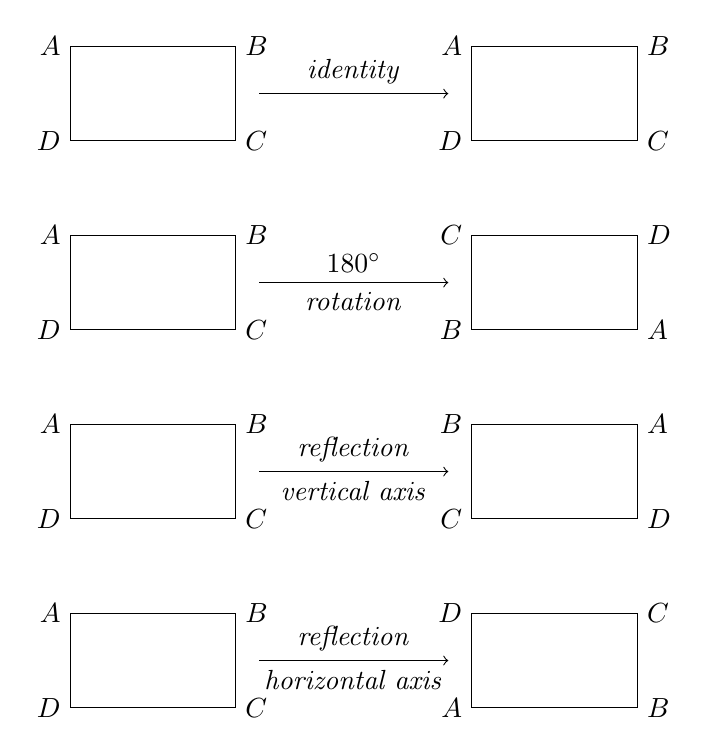
\begin{tikzpicture}[scale=1.2]
\draw (-3,0) -- (-1.25,0) -- (-1.25,1) -- (-3,1) -- cycle;
\draw (3,0) -- (1.25,0) -- (1.25,1) -- (3,1) -- cycle;
\draw [->] (-1,0.5) -- (1,0.5);
\node [above] at (0,0.5) {\emph{reflection}};
\node [below] at (0,0.5) {\emph{horizontal axis}};
\node [above,left] at (-3,1) {$A$};
\node [below,left] at (-3,0) {$D$};
\node [above,right] at (-1.25,1) {$B$};
\node [below,right] at (-1.25,0) {$C$};
\node [above,right] at (3,1) {$C$};
\node [below,right] at (3,0) {$B$};
\node [above,left] at (1.25,1) {$D$};
\node [below,left] at (1.25,0) {$A$};

\draw (-3,2) -- (-1.25,2) -- (-1.25,3) -- (-3,3) -- cycle;
\draw (3,2) -- (1.25,2) -- (1.25,3) -- (3,3) -- cycle;
\draw [->] (-1,2.5) -- (1,2.5);
\node [above] at (0,2.5) {\emph{reflection}};
\node [below] at (0,2.5) {\emph{vertical axis}};
\node [above,left] at (-3,3) {$A$};
\node [below,left] at (-3,2) {$D$};
\node [above,right] at (-1.25,3) {$B$};
\node [below,right] at (-1.25,2) {$C$};
\node [above,right] at (3,3) {$A$};
\node [below,right] at (3,2) {$D$};
\node [above,left] at (1.25,3) {$B$};
\node [below,left] at (1.25,2) {$C$};

\draw (-3,4) -- (-1.25,4) -- (-1.25,5) -- (-3,5) -- cycle;
\draw (3,4) -- (1.25,4) -- (1.25,5) -- (3,5) -- cycle;
\draw [->] (-1,4.5) -- (1,4.5);
\node [above] at (0,4.5) {$180^\circ$};
\node [below] at (0,4.5) {\emph{rotation}};
\node [above,left] at (-3,5) {$A$};
\node [below,left] at (-3,4) {$D$};
\node [above,right] at (-1.25,5) {$B$};
\node [below,right] at (-1.25,4) {$C$};
\node [above,right] at (3,5) {$D$};
\node [below,right] at (3,4) {$A$};
\node [above,left] at (1.25,5) {$C$};
\node [below,left] at (1.25,4) {$B$};

\draw (-3,6) -- (-1.25,6) -- (-1.25,7) -- (-3,7) -- cycle;
\draw (3,6) -- (1.25,6) -- (1.25,7) -- (3,7) -- cycle;
\draw [->] (-1,6.5) -- (1,6.5);
\node [above] at (0,6.5) {\emph{identity}};
\node [above,left] at (-3,7) {$A$};
\node [below,left] at (-3,6) {$D$};
\node [above,right] at (-1.25,7) {$B$};
\node [below,right] at (-1.25,6) {$C$};
\node [above,right] at (3,7) {$B$};
\node [below,right] at (3,6) {$C$};
\node [above,left] at (1.25,7) {$A$};
\node [below,left] at (1.25,6) {$D$};

\end{tikzpicture}
\end{center}
\end{figure}

A \boldemph{symmetry} of a geometric figure is a rearrangement of the figure preserving the arrangement of its sides and vertices as well as its distances and angles.  A map from the plane to itself preserving the symmetry of an object is called a \boldemph{rigid motion}\index{Rigid motion}.  For example, if we look at the rectangle in Figure~\ref{groups_figure_rectangle}, it is easy to see that a rotation of $180^{\circ}$ or $360^{\circ}$ returns a rectangle in the plane with the same orientation as the original rectangle and the same relationship among the vertices.  A reflection of the rectangle across either the vertical axis or the horizontal axis can also be seen to be a symmetry.  However, a $90^{\circ}$ rotation in either direction cannot be a symmetry unless the rectangle is a square.





\begin{figure}[hbt] %Replaced diagram with a tikz figure - TWJ 5/5/2010

\begin{center}
\caption{Symmetries of a triangle}\label{S3_Symmetry_Figure}
\bigskip

\tikzpreface{groups_s3_symmetry}
\begin{tikzpicture}[scale=0.7]
\draw (0,0) -- (0:2) -- (60:2) -- cycle;
\node [left] at (0,0) {$A$};
\node at (1,2.1) {$B$};
\node [right] at (0:2) {$C$};

\draw [->] (2,1) -- (4,1);
\node [above] at (3,1) {\emph{reflection}};

\draw (4,0) -- (0:6) -- ++(120:2) -- cycle;
\node [left] at (4,0) {$B$};
\node [right] at (0:6) {$C$};
\node at (5,2.1) {$A$};

\node [right] at (7,1) {$ \mu_3 = \begin{pmatrix} A & B & C \\ B & A & C \end{pmatrix}$};

\draw (0,3) -- (2,3) -- ++(120:2) -- cycle;
\node [left] at (0,3) {$A$};
\node at (1,5.1) {$B$};
\node [right] at (2,3) {$C$};

\draw [->] (2,4) -- (4,4);
\node [above] at (3,4) {\emph{reflection}};

\draw (4,3) -- (6,3) -- ++(120:2) -- cycle;
\node [left] at (4,3) {$C$};
\node [right] at (6,3) {$A$};
\node at (5,5.1) {$B$};
\node [right] at (7,4) {$ \mu_2 = \begin{pmatrix} A & B & C \\ C & B & A \end{pmatrix}$};

\draw (0,6) -- (2,6) -- ++(120:2) -- cycle;
\node [left] at (0,6) {$A$};
\node at (1,8.1) {$B$};
\node [right] at (2,6) {$C$};

\draw [->] (2,7) -- (4,7);
\node [above] at (3,7) {\emph{reflection}};

\draw (4,6) -- (6,6) -- ++(120:2) -- cycle;
\node [left] at (4,6) {$A$};
\node [right] at (6,6) {$B$};
\node at (5,8.1) {$C$};
\node [right] at (7,7) {$ \mu_1 = \begin{pmatrix} A & B & C \\ A & C & B \end{pmatrix}$};

\draw (0,9) -- (2,9) -- ++(120:2) -- cycle;
\node [left] at (0,9) {$A$};
\node at (1,11.1) {$B$};
\node [right] at (2,9) {$C$};

\draw [->] (2,10) -- (4,10);
\node [above] at (3,10) {\emph{rotation}};

\draw (4,9) -- (6,9) -- ++(120:2) -- cycle;
\node [left] at (4,9) {$B$};
\node [right] at (6,9) {$A$};
\node at (5,11.1) {$C$};
\node [right] at (7,10) {$ \rho_2 = \begin{pmatrix} A & B & C \\ C & A & B \end{pmatrix}$};

\draw (0,12) -- (2,12) -- ++(120:2) -- cycle;
\node [left] at (0,12) {$A$};
\node at (1,14.1) {$B$};
\node [right] at (2,12) {$C$};

\draw [->] (2,13) -- (4,13);
\node [above] at (3,13) {\emph{rotation}};

\draw (4,12) -- (6,12) -- ++(120:2) -- cycle;
\node [left] at (4,12) {$C$};
\node [right] at (6,12) {$B$};
\node at (5,14.1) {$A$};
\node [right] at (7,13) {$ \rho_1 = \begin{pmatrix} A & B & C \\ B & C & A  \end{pmatrix}$};

\draw (0,15) -- (2,15) -- ++(120:2) -- cycle;
\node [left] at (0,15) {$A$};
\node at (1,17.1) {$B$};
\node [right] at (2,15) {$C$};

\draw [->] (2,16) -- (4,16);
\node [above] at (3,16) {\emph{identity}};

\draw (4,15) -- (6,15) -- ++(120:2) -- cycle;
\node [left] at (4,15) {$A$};
\node [right] at (6,15) {$C$};
\node at (5,17.1) {$B$};
\node [right] at (7,16) {$ id = \begin{pmatrix} A & B & C \\ A & B & C  \end{pmatrix}$};


\end{tikzpicture}
\end{center}
\end{figure}


Let us find the symmetries of the equilateral triangle $\bigtriangleup ABC$.  To find a symmetry of $\bigtriangleup ABC$, we must first examine the permutations of the vertices $A$, $B$, and $C$ and then ask if a permutation extends to a symmetry of the triangle.  Recall that a \boldemph{permutation} of a set $S$ is a one-to-one and onto map $\pi :S \rightarrow S$.  The three vertices have $3! = 6$ permutations, so the triangle has at most six symmetries.  To see that there are six permutations, observe there are three different possibilities for the first vertex, and two for the second, and the remaining vertex is determined by the placement of the first two.  So we have $3 \cdot 2 \cdot 1 = 3! = 6$ different arrangements.  To denote the permutation of the vertices of an equilateral triangle that sends $A$ to $B$, $B$ to $C$, and $C$ to $A$, we write the array
\[
\begin{pmatrix}
A & B & C \\
B & C & A
\end{pmatrix}.
\]
Notice that this particular permutation corresponds to the rigid motion of rotating the triangle by $120^{\circ}$ in a clockwise direction.  In fact, every permutation gives rise to a symmetry of the triangle.  All of these symmetries are shown in Figure~\ref{S3_Symmetry_Figure}.

 
A natural question to ask is what happens if one motion of the triangle $\bigtriangleup ABC$ is followed by another.  Which symmetry is $\mu_1 \rho_1$; that is, what happens when we do the permutation $\rho_1$ and then the permutation $\mu_1$?  \emph{Remember that we are composing functions here.  Although we usually multiply left to right, we compose functions right to left.} We have
\begin{align*}
(\mu_1 \rho_1)(A)  & = \mu_1( \rho_1( A ) ) = \mu_1( B ) = C \\
(\mu_1 \rho_1)(B) & = \mu_1( \rho_1( B ) ) = \mu_1( C ) = B \\
(\mu_1 \rho_1)(C) & = \mu_1( \rho_1( C ) ) = \mu_1( A ) = A.
\end{align*}
This is the same symmetry as $\mu_2$.  Suppose we do these motions in the opposite order, $\rho_1$ then $\mu_1$.  It is easy to determine that this is the same as the symmetry $\mu_3$; hence, $\rho_1 \mu_1 \neq \mu_1 \rho_1$.  A multiplication table for the symmetries of an equilateral triangle $\bigtriangleup ABC$ is given in Table~\ref{S3_table}.

Notice that in the multiplication table for the symmetries of an equilateral triangle, for every motion of the triangle $\alpha$ there is another motion $\alpha'$ such that $\alpha \alpha' = id$;  that is, for every motion there is another  motion that takes the triangle back to its original orientation.  

\begin{table}
\caption{Symmetries of an equilateral triangle}{\small
\begin{center}
\begin{tabular}{c|cccccc}
$\circ$  & $id$     & $\rho_1$ & $\rho_2$ & $\mu_1$ & $\mu_2$ & $\mu_3$ \\
\hline
$id$     & $id$     & $\rho_1$ & $\rho_2$ & $\mu_1$ & $\mu_2$ & $\mu_3$ \\
$\rho_1$ & $\rho_1$ & $\rho_2$ & $id$     & $\mu_3$ & $\mu_1$ & $\mu_2$ \\
$\rho_2$ & $\rho_2$ & $id$     & $\rho_1$ & $\mu_2$ & $\mu_3$ & $\mu_1$ \\
$\mu_1$  & $\mu_1$  & $\mu_2$  & $\mu_3$  & $id$    & $\rho_1$& $\rho_2$\\
$\mu_2$  & $\mu_2$  & $\mu_3$  & $\mu_1$  & $\rho_2$& $id$    & $\rho_1$\\
$\mu_3$  & $\mu_3$  & $\mu_1$  & $\mu_2$  & $\rho_1$& $\rho_2$& $id$
\end{tabular}
\end{center}
}
\label{S3_table}
\end{table}
 
 
\section{Definitions and Examples}\label{groups_section_define}

%% TWJ, 2010/03/31
%% Fixed the error  $(a,b) \in G \times G$
 
The integers mod $n$ and the symmetries of a triangle or a rectangle are both examples of groups.  A \boldemph{binary operation}\index{Binary operation} or \boldemph{law of composition} on a set $G$ is a function $G \times G \rightarrow G$ that assigns to each pair $(a,b) \in G \times G$ a unique element $a \circ b$, or $ab$ in $G$, called the composition of $a$ and $b$.  A \boldemph{group}\index{Group!definition of} $(G, \circ )$ is a set $G$ together with a law of composition $(a,b) \mapsto a \circ b$ that satisfies the following axioms. 
\begin{itemize}
 
\item
The law of composition is \boldemph{associative}. That is,
\[
(a \circ b) \circ c = a \circ (b \circ c)
\]
for $a, b, c \in G$.
 
\item
There exists an element $e \in G$, called the \boldemph{identity element}\index{Element!identity}, such that for any element $a \in G$ 
\[
e \circ a = a \circ e = a.
\]
 
\item
For each element $a \in G$, there exists an \boldemph{inverse element}\index{Element!inverse} in G, denoted by $a^{-1}$, such that 
\[
a \circ a^{-1} = a^{-1} \circ a = e.
\]
\end{itemize}
A group $G$ with the property that $a \circ b = b \circ a$ for all $a, b \in G$ is called \boldemph{abelian}\index{Abelian group}\index{Group!abelian} or \boldemph{commutative}\index{Group!commutative}.  Groups not satisfying this property are said to be  \boldemph{nonabelian}\index{Group!nonabelian} or \boldemph{noncommutative}\index{Group!noncommutative}.  

\begin{example}{group_integers}
The integers ${\mathbb Z } = \{ \ldots , -1, 0, 1, 2, \ldots \}$ form a group under the operation of addition.  The binary operation on two integers $m, n \in {\mathbb Z}$ is just their sum.  Since the integers under addition already have a well-established notation, we will use the operator $+$ instead of $\circ$; that is, we shall write $m + n$ instead of $m \circ n$.  The identity is 0, and the inverse of $n \in {\mathbb Z}$ is written as $-n$ instead of $n^{-1}$.  Notice that the integers under addition have the additional property that $m + n = n + m$ and are therefore an abelian group.   
\end{example}

Most of the time we will write $ab$ instead of $a \circ b$; however, if the group already has a natural operation such as addition in the integers, we will use that operation.  That is, if we are adding two integers, we still write $m + n$, $-n$ for the inverse, and 0 for the identity as usual. We also write $m - n$ instead of $m + (-n)$.

\begin{table}[htb]
\caption{Cayley table for $({\mathbb Z}_5, +)$}{\small
\begin{center}
\begin{tabular}{c|ccccc}
$+$ & 0 & 1 & 2 & 3 & 4 \\
\hline
  0 & 0 & 1 & 2 & 3 & 4 \\
  1 & 1 & 2 & 3 & 4 & 0 \\
  2 & 2 & 3 & 4 & 0 & 1 \\
  3 & 3 & 4 & 0 & 1 & 2 \\
  4 & 4 & 0 & 1 & 2 & 3
\end{tabular}
\end{center}\label{Z5_Cayley_Table}
}
\end{table}
 
It is often convenient to describe a group in terms of an addition or multiplication table.  Such a table is called a \boldemph{Cayley table}\index{Cayley table}.

\medskip
 
\begin{example}{Z5_group}
The integers mod $n$ form a group under addition modulo $n$.  Consider ${\mathbb Z}_5$, consisting of the equivalence classes of the integers 0, 1, 2, 3, and 4.  We define the group operation on ${\mathbb Z}_5$ by modular addition.  We write the binary operation on the group additively; that is, we write $m + n$.  The element 0 is the identity of the group and each element in ${\mathbb Z}_5$ has an inverse. For instance, $2 + 3 = 3 + 2 = 0$.  Table~\ref{Z5_Cayley_Table} is a Cayley table for ${\mathbb Z}_5$.  By Proposition~\ref{Zn_equiv_classes}, ${\mathbb Z}_n = \{0, 1, \ldots, n-1 \}$ is a group under the binary operation of addition mod $n$.  
\end{example}

\begin{example}{Z6_Mult}
Not every set with a binary operation is a group.  For example, if we let modular multiplication be the binary operation on ${\mathbb Z}_n$, then ${\mathbb Z}_n$ fails to be a group.  The element 1 acts as a group identity since $1 \cdot k = k \cdot 1 = k$ for any $k \in {\mathbb Z}_n$; however, a multiplicative inverse for $0$ does not exist since $0 \cdot k = k \cdot 0 = 0$ for every $k$ in ${\mathbb Z}_n$.  Even if we consider the set ${\mathbb Z}_n \setminus \{0 \}$, we still may not have a group.  For instance, let $2 \in {\mathbb Z}_6$. Then 2 has no multiplicative inverse since 
\begin{align*}
0 \cdot 2 & = 0 \qquad 1 \cdot 2 = 2 \\
2 \cdot 2 & = 4 \qquad 3 \cdot 2 = 0 \\
4 \cdot 2 & = 2 \qquad 5 \cdot 2 = 4.
\end{align*}
By Proposition~\ref{Zn_equiv_classes}, every nonzero $k$ does have an inverse in ${\mathbb Z}_n$ if $k$ is relatively prime to $n$.  Denote the set of all such nonzero elements in ${\mathbb Z}_n$ by $U(n)$\label{groupofunits}.  Then $U(n)$ is a group called the \boldemph{group of units}\index{Group!of units} of ${\mathbb Z}_n$.  Table~\ref{cayley_table_U8} is a Cayley table for the group $U(8)$. 
\end{example}

\begin{table}[htb]
\caption{Multiplication table for $U(8)$}{\small
\begin{center}
\begin{tabular}{c|cccc}
$\cdot$ & 1 & 3 & 5 & 7 \\
\hline
1       & 1 & 3 & 5 & 7 \\
3       & 3 & 1 & 7 & 5 \\
5       & 5 & 7 & 1 & 3 \\
7       & 7 & 5 & 3 & 1
\end{tabular}
\end{center}
}
\label{cayley_table_U8}
\end{table}



\begin{example}{nonabelian}
The symmetries of an equilateral triangle described in Section~\ref{Section_mod_N_sym} form a nonabelian group. As we observed, it is not necessarily true that $\alpha \beta = \beta \alpha$ for two symmetries $\alpha$ and $\beta$.  Using Table~\ref{S3_table}, which is a Cayley table for this group, we can easily check that the symmetries of an equilateral triangle are indeed a group. We will denote this group by either $S_3$ or $D_3$, for reasons that will be explained later. 
\end{example}



\begin{example}{GL2}
We use  ${\mathbb M}_2 ( {\mathbb R})$\label{notematrices} to denote the set of all $2 \times 2$ matrices.  Let $GL_2({\mathbb R})$ be the subset of ${\mathbb M}_2 ( {\mathbb R})$ consisting of invertible matrices; that is, a matrix 
\[
A =
\begin{pmatrix}
a & b \\
c & d
\end{pmatrix}
\]
is in  $GL_2( {\mathbb R})$ if there exists a matrix $A^{-1}$ such that
$A A^{-1} = A^{-1} A = I$, where $I$ is the $2 \times 2$ identity
matrix. For $A$ to have an inverse is equivalent to requiring that the
determinant of $A$ be nonzero; that is, $\det A = ad - bc \neq
0$\label{determinant}. The set of invertible matrices forms a group
called the \boldemph{general linear group}\index{Group!general
linear}\label{generallinear}. The identity of the group is the
identity matrix  
\[
I =
\begin{pmatrix}
1 & 0 \\
0 & 1
\end{pmatrix}.
\]
The inverse of $A \in GL_2( {\mathbb R})$ is
\[
A^{-1} =
\frac{1}{ad-bc}
\begin{pmatrix}
d & -b \\
-c & a
\end{pmatrix}.
\]
The product of two invertible matrices is again invertible. Matrix
multiplication is associative, satisfying the other group axiom. For
matrices it is not true in general that $AB = BA$; hence, $GL_2(
{\mathbb R})$ is another example of a nonabelian group.
\end{example}

%% Changed $AB \neq BA$ to $AB = BA$. Suggested by Isaac Coombs. TWJ 8/24/2011

 
 
\begin{example}{quaterions}
Let
\begin{align*}
1
& = 
\begin{pmatrix}
1 & 0 \\
0 & 1
\end{pmatrix}
\qquad
I
=
\begin{pmatrix}
0 & 1 \\
-1 & 0
\end{pmatrix}
\\
J
& = 
\begin{pmatrix}
0 & i \\
i & 0
\end{pmatrix}
\qquad
K =
\begin{pmatrix}
i & 0 \\
0 & -i
\end{pmatrix},
\end{align*}
where $i^2 = -1$. Then the relations $I^2 = J^2 = K^2 = -1$, $IJ=K$,
$JK=I$, $KI=J$, $JI=-K$, $KJ=-I$, and $IK=-J$ hold. The set
$Q_8\label{notequateriongroup} = \{
\pm 1, \pm I, \pm J, \pm K  \}$ is a group called the \boldemph{quaternion
group}\index{Group!quaternion}\index{Quaternions}. Notice that  $Q_8$
is noncommutative. 
\end{example}
 
 
\begin{example}{C_star}
Let ${\mathbb C}^\ast$\label{noteCstar} be the set of nonzero complex 
numbers. Under the
operation of multiplication ${\mathbb C}^\ast$ forms a group.  The
identity is 1. If $z = a+bi$ is a nonzero complex number, then
\[
z^{-1} = \frac{a -bi}{a^2 +b^2}
\]
is the inverse of $z$.  It is easy to see that the remaining group
axioms hold. 
\end{example}
 
 

 
 
A group is \boldemph{finite}\index{Group!finite}, or has \boldemph{finite
order}, if it contains a finite number of elements; otherwise, the
group is said to be \boldemph{infinite} or to have \boldemph{infinite
order}\index{Group!infinite}. The \boldemph{order}\index{Group!order of}
of a finite group is the number of elements that it contains. If $G$
is a group containing $n$ elements, we write $|G| =
n$\label{noteorder}. The group ${\mathbb Z}_5$ is a finite group of order
5; the integers ${\mathbb Z}$ form an infinite group under addition, and
we sometimes write $|{\mathbb Z}| = \infty$.
 
 
\subsection*{Basic Properties of Groups}
 
 
\begin{proposition}
The identity element in a group $G$ is unique; that is, there exists
only one element $e \in G$ such that $eg = ge = g$ for all $g \in G$. 
\end{proposition}
 
 
\begin{proof}
Suppose that $e$ and $e'$ are both identities in $G$. Then $eg = ge =
g$ and $e'g = ge' = g$ for all $g \in G$. We need to show that $e =
e'$. If we think of $e$ as the identity, then $ee' = e'$; but if $e'$
is the identity, then $ee' = e$. Combining these two equations, we
have $e = ee' = e'$. 
\end{proof}
 
 
\medskip
 
 
Inverses in a group are also unique. If $g'$ and $g''$ are both
inverses of an element $g$ in a group $G$, then $gg' = g'g = e$ and
$gg'' = g''g = e$. We want to show that $g' = g''$, but $g' = g'e =
g'(gg'') = (g'g)g'' = eg'' = g''$. We summarize this fact in the
following proposition. 
 
 
\begin{proposition}
If $g$ is any element in a group $G$, then the inverse of $g$,
$g^{-1}$, is unique. 
\end{proposition}
 
 
\begin{proposition}
Let $G$ be a group. If $a, b \in G$, then $(ab)^{-1} = b^{-1}a^{-1}$. 
\end{proposition}
 
 
\begin{proof}
Let $a, b \in G$. Then $abb^{-1}a^{-1} = aea^{-1} = aa^{-1} = e$.
Similarly, $b^{-1}a^{-1}ab = e$. But by the previous proposition,
inverses are unique; hence, $(ab)^{-1} = b^{- 1}a^{-1}$.
\end{proof}
 
 
\begin{proposition}
Let $G$ be a group.  For any $a \in G$, $(a^{-1})^{-1} = a$.
\end{proposition}
 
 
\begin{proof}
Observe that $a^{-1} (a^{-1})^{-1} = e$. Consequently, multiplying
both sides of this equation by $a$, we have 
\[
(a^{-1})^{-1} = e (a^{-1})^{-1} = a a^{-1} (a^{-1})^{-1} = ae = a.
\]
\end{proof}
 
 
\medskip
 
 
It makes sense to write equations with group elements and group
operations. If $a$ and $b$ are two elements in a group $G$, does there 
exist an element $x \in G$ such that $ax = b$? If such an $x$ does
exist, is it unique? The following proposition answers both of these
questions positively. 
 
 
\begin{proposition}\label{group_equations}
Let $G$ be a group and $a$ and $b$ be any two elements in $G$. Then
the equations $ax = b$ and $xa = b$ have unique solutions in $G$. 
\end{proposition}
 
 
\begin{proof}
Suppose that $ax = b$. We must show that such an $x$ exists.
Multiplying both sides of $ax = b$ by $a^{-1}$, we have $x = ex =
a^{-1}ax = a^{-1}b$. 
 
 
To show uniqueness, suppose that $x_1$ and $x_2$ are both solutions of
$ax = b$; then $ax_1 = b = ax_2$. So $x_1 = a^{-1}ax_1 = a^{-1}ax_2 =
x_2$. The proof for the existence and uniqueness of the solution of
$xa = b$ is similar. 
\end{proof}
 

 
\begin{proposition}
If $G$ is a group and $a, b, c \in G$, then $ba = ca$ implies $b = c$
and $ab = ac$ implies $b = c$. 
\end{proposition} 
 
This proposition tells us that the \boldemph{right and 
left cancellation laws}\index{Cancellation law!for
groups} are true in groups.  We leave the proof as an exercise.
 
 
We can use exponential notation for groups just as we do in ordinary
algebra. If $G$ is a group and $g \in G$, then we define $g^0 = e$.
For $n \in {\mathbb N}$, we define 
\[
g^n = \underbrace{g \cdot g \cdots g}_{n \; {\rm times}}
\]
and
\[
g^{-n} = \underbrace{g^{-1} \cdot g^{-1} \cdots g^{-1}}_{n
\; {\rm times}}.
\]
 
 
\begin{theorem}\label{exponent_laws}
In a group, the usual laws of exponents hold; that is, for all $g, h
\in G$,
\begin{enumerate}
 
\rm \item \it
$g^mg^n = g^{m+n}$ for all $m, n \in {\mathbb Z}$; 
 
\rm \item \it
$(g^m)^n = g^{mn}$ for all $m, n \in {\mathbb Z}$; 
 
\rm \item \it
$(gh)^n = (h^{-1}g^{-1})^{-n}$ for all $n \in {\mathbb Z}$. Furthermore,
if $G$ is abelian, then $(gh)^n = g^nh^n$. 
 
\end{enumerate}
\end{theorem}
 
 
We will leave the proof of this theorem as an exercise. Notice that
$(gh)^n \neq g^nh^n$ in general, since the group may not be abelian.
If the group is ${\mathbb Z}$ or ${\mathbb Z}_n$, we write the group
operation additively and the exponential operation multiplicatively;
that is, we write $ng$ instead of $g^n$. The laws of exponents now
become 
\begin{enumerate}
 
\item
$mg + ng = (m+n)g$ for all $m, n \in {\mathbb Z}$;
 
\item
$m(ng) = (mn)g$ for all $m, n \in {\mathbb Z}$;
 
\item
$m(g + h) = mg + mh$ for all $n \in {\mathbb Z}$.
 
\end{enumerate}
It is important to realize that the last statement can be made only
because ${\mathbb Z}$ and  ${\mathbb Z}_n$ are commutative groups.
 
 
 
 
\histhead
 
 
\noindent
{\small \histf
Although the first clear axiomatic definition of a group was not given
until the late 1800s,  group-theoretic methods had been employed
before this time in the development of  many areas of mathematics,
including geometry and the theory of algebraic equations.  
 

Joseph-Louis Lagrange\index{Lagrange, Joseph-Louis} used
group-theoretic methods in a 1770--1771 memoir to study methods of
solving polynomial equations.  Later, \'{E}variste
Galois\index{Galois, \'{E}variste} (1811--1832) succeeded in
developing the mathematics necessary to determine exactly which
polynomial equations could be  solved in terms of the polynomials'
coefficients. Galois' primary tool was group theory. 
}

{\small \histf
The study of geometry was revolutionized in 1872 when Felix
Klein\index{Klein, Felix} proposed that geometric spaces should be
studied by examining those properties that are invariant under a
transformation of the space. Sophus Lie\index{Lie, Sophus}, a
contemporary of Klein, used group theory to study solutions of
partial differential equations.  One of the first modern treatments of
group theory appeared in William Burnside's\index{Burnside, William}
\textit{The Theory of Groups of Finite Order} [1], first published in
1897.  
\histbox
}


 
 
 
\section{Subgroups}\label{groups_section_subgroups}
 
 
\subsection*{Definitions and Examples}
 
 
Sometimes we wish to investigate smaller groups sitting
inside a larger group.   The set of even integers $2{\mathbb Z} = \{
\ldots, -2, 0, 2, 4, \ldots \}$ is a group  under the operation of
addition. This smaller group sits naturally inside of the group of
integers under addition.  We define a \boldemph{
subgroup}\index{Subgroup!definition of} $H$ of a group $G$ to be a
subset $H$ of $G$ such that when the group operation of $G$ is
restricted to $H$, $H$ is a group in its own right. 
Observe that every group $G$ with at least two elements will always
have at least two subgroups, the subgroup consisting of the identity
element alone and the entire group itself. The subgroup $H = \{ e \}$
of a group $G$ is called the \boldemph{trivial
subgroup}\index{Subgroup!trivial}.  A subgroup that is a proper subset
of $G$ is called a \boldemph{proper subgroup}\index{Subgroup!proper}. In
many of the examples that we have investigated up to this point, there
exist other subgroups besides the trivial and improper subgroups.  
 
 
\begin{example}{multiplicative_subgroup}
Consider the set of nonzero real numbers, ${\mathbb
R}^*$,\label{noteRstar}  with the group operation of multiplication.
The identity of this group is 1 and the inverse of any element $a \in
{\mathbb R}^*$ is just $1/a$. We will  show  that
\[
{\mathbb Q}^*\label{noteQstar} = \{ p/q : p \, {\rm
and }\, q\, {\rm are\, nonzero\, integers} \}
\]
is a subgroup of ${\mathbb R}^*$. The identity of ${\mathbb R}^*$ is 1;
however,  $1 = 1/1$ is the quotient of two nonzero integers. Hence,
the identity of ${\mathbb R}^*$ is in ${\mathbb Q}^*$. Given two elements in
${\mathbb Q}^*$, say $p/q$ and $r/s$, their product $pr/qs$ is also in
${\mathbb Q}^*$. The inverse of any element $p/q \in {\mathbb Q}^*$ is again
in ${\mathbb Q}^*$ since $(p/q)^{-1} = q/p$. Since multiplication in
${\mathbb R}^*$ is associative, multiplication in ${\mathbb Q}^*$ is
associative. 
\end{example}
 
 
\begin{example}{subgroup_H}
Recall that ${\mathbb C}^{\ast}$  is the multiplicative group of nonzero
complex numbers. Let $H = \{ 1, -1, i, -i \}$. Then $H$ is a subgroup
of ${\mathbb C}^{\ast}$. It is quite easy to verify  that $H$ is a group
under multiplication and that $H \subset {\mathbb C}^{\ast}$. 
\end{example}
 
 
\begin{example}{SL2}
Let $SL_2( {\mathbb R})$\label{speciallinear} be the subset of $GL_2( {\mathbb R })$
consisting of matrices of determinant one; that is, a matrix
\[
A =
\begin{pmatrix}
a & b \\
c & d
\end{pmatrix}
\]
is in $SL_2( {\mathbb R})$ exactly when $ad - bc = 1$. To show that
$SL_2( {\mathbb R})$ is a subgroup of the general linear group, we must
show that it is a group under matrix multiplication.  The $2 \times 2$
identity matrix is in $SL_2( {\mathbb R})$, as is the inverse of the
matrix $A$:  
\[
A^{-1} =
\begin{pmatrix}
d  & -b \\
-c &  a
\end{pmatrix}.
\]
It remains to show that multiplication is closed; that is, that the
product of two matrices of determinant one also has determinant one.
We will leave this task as an exercise. The group $SL_2({\mathbb R})$ is
called the \boldemph{special linear group}\index{Group!special
linear}.
\end{example}
 
 
\begin{example}{GL2_subgroup}
It is important to realize that a subset $H$ of a group $G$ can be a
group without being a subgroup of $G$. For $H$ to be a subgroup of $G$
it must inherit $G$'s binary operation.  The set of all $2 \times 2$ 
matrices, ${\mathbb M}_2(\mathbb R)$, forms a group under the operation of
addition. The $2 \times 2$ general linear group is a subset of ${\mathbb
M}_2(\mathbb R)$ and is a group under matrix multiplication, but it is not a
subgroup of ${\mathbb M}_2(\mathbb R)$.  If we add two invertible matrices,
we do not necessarily obtain another invertible matrix. Observe that 
\[
\begin{pmatrix}
1 & 0 \\
0 & 1
\end{pmatrix}
+
\begin{pmatrix}
-1 &  0 \\
0  & -1
\end{pmatrix}
=
\begin{pmatrix}
0 & 0 \\
0 & 0
\end{pmatrix},
\]
but the zero matrix is not in $GL_2( {\mathbb R })$.
\end{example}
 
 
\begin{example}{Z2xZ2}
One way of telling whether or not two groups are the same is by
examining their subgroups.  Other than the trivial subgroup and the
group itself, the group ${\mathbb Z}_4$ has a single subgroup consisting
of the elements 0 and 2. From the group ${\mathbb Z}_2$, we can form
another group of four elements as follows.  As a set this group is
${\mathbb Z}_2 \times {\mathbb Z}_2$. We perform the group operation 
coordinatewise; that is, $(a,b) + (c,d) = (a+c, b+d)$. Table~\ref{groups:table_Z2xZ2} is
an addition table for ${\mathbb Z}_2 \times {\mathbb Z}_2$. Since
there are three nontrivial proper subgroups of ${\mathbb Z}_2 \times
{\mathbb Z}_2$, $H_1 = \{ (0,0), (0,1) \}$, $H_2 = \{ (0,0), (1,0) \}$,
and $H_3 = \{ (0,0), (1,1) \}$, ${\mathbb Z}_4$ and ${\mathbb Z}_2 \times
{\mathbb Z}_2$ must be different groups.
\end{example}
 
 
\begin{table}[htb]

{\small
\begin{center}
\begin{tabular}{c|cccc}
$+$     & (0,0) & (0,1) & (1,0) & (1,1) \\
\hline
(0,0) & (0,0) & (0,1) & (1,0) & (1,1) \\
(0,1) & (0,1) & (0,0) & (1,1) & (1,0) \\
(1,0) & (1,0) & (1,1) & (0,0) & (0,1) \\
(1,1) & (1,1) & (1,0) & (0,1) & (0,0)
\end{tabular}
\end{center}
}
\caption{Addition table for ${\mathbb Z}_2 \times {\mathbb Z}_2$}\label{groups:table_Z2xZ2}
\end{table} 
 
 
\subsection*{Some Subgroup Theorems}
 
 
Let us examine some criteria for determining exactly when a subset of
a group is a subgroup.
 
 
\begin{proposition}
A subset $H$ of $G$ is a subgroup if and only if it satisfies the
following conditions. 
\begin{enumerate}
 
\rm \item \it 
The identity $e$ of $G$ is in $H$. 
 
\rm \item \it 
If $h_1, h_2 \in H$, then $h_1h_2 \in H$. 
 
\rm \item \it 
If $h \in H$, then $h^{-1} \in H$.
 
\end{enumerate}
\end{proposition}
 
 
\begin{proof}
First suppose that $H$ is a subgroup of $G$.  We must show that the three conditions hold.  Since $H$ is a group, it must have an identity $e_H$.  We must show that $e_H = e$, where $e$ is the identity of $G$. We know that $e_H e_H = e_H$ and that $ee_H = e_H e = e_H$; hence, $ee_H = e_H e_H$.  By right-hand cancellation, $e =e_H$.  The second condition holds since a subgroup $H$ is a group.  To prove the third condition, let $h \in H$.  Since $H$ is a group, there is  an element $h' \in H$ such that $hh' = h'h = e$.  By the uniqueness  of the inverse in $G$, $h' = h^{-1}$.

Conversely, if the three conditions hold, we must show that $H$ is a group under the same operation as $G$; however, these conditions plus the associativity of the binary operation are exactly the axioms stated in the definition of a group.
\end{proof}

\begin{proposition}\label{groups:subgroup_prop}
Let $H$ be a subset of a group $G$.  Then $H$ is a subgroup of $G$ if and only if $H \neq \emptyset$, and whenever $g, h \in H$ then $gh^{-1}$ is in $H$. 
\end{proposition}
 
 
\begin{proof}
First assume that $H$ is a subgroup of $G$.  We wish to show that $gh^{-1} \in H$ whenever $g$ and $h$ are in $H$.  Since $h$ is in $H$, its inverse $h^{-1}$ must also be in $H$.  Because of the closure of the group operation, $gh^{-1} \in H$. 

Conversely, suppose that $H \subset G$ such that $H \neq \emptyset$ and  $g h^{-1} \in H$ whenever $g, h \in H$.  If $g \in H$, then $gg^{-1} = e$ is in $H$.  If $g \in H$, then $eg^{-1} = g^{-1}$ is also in $H$. Now let $h_1, h_2 \in H$. We must show that their product is also in $H$.  However, $h_1(h_2^{-1})^{-1} = h_1 h_2 \in H$.  Hence, $H$ is a subgroup of $G$. 
\end{proof}

%% TWJ, 2012/11/21
%% Proof rewritten for clarity.  Suggested by R. Beezer.

%Let $H$ be a nonempty subset of $G$.  Then $H$ contains some element $g$.  So $gg^{-1} = e$ is in $H$.  If $g \in H$, then $eg^{-1} = g^{-1}$ is also in $H$. Finally, let $g, h \in H$. We must show that their product is also in $H$.  However, $g(h^{-1})^{-1} = gh \in H$.  Hence, $H$ is indeed a subgroup of $G$. Conversely, if $g$ and $h$ are in $H$, we want to show that $gh^{-1} \in H$.  Since $h$ is in $H$, its inverse $h^{-1}$ must also be in $H$.  Because of the closure of the group operation, $gh^{-1} \in H$. 
%\end{proof}
 
 
\markright{EXERCISES}
\section*{Exercises}
\exrule

{\small
\begin{enumerate}

\item
Find all $x \in {\mathbb Z}$ satisfying each of the following equations.
\begin{multicols}{2}
\begin{enumerate}

\item 
$3x \equiv 2 \pmod{ 7}$

\item
$5x + 1 \equiv 13 \pmod{ 23}$

\item
$5x + 1 \equiv 13 \pmod{ 26}$

\item
$9x \equiv 3 \pmod{ 5}$

\item
$5x \equiv 1 \pmod{ 6}$

\item
$3x \equiv 1 \pmod{ 6}$

\end{enumerate}
\end{multicols}
  

 
 \item   %%%%%%%%%%%%%%%%%%%%%%%%%
Which of the following multiplication tables defined on the set $G =
\{ a, b, c, d \}$ form a group? Support your answer in each case. 
\begin{multicols}{2}
\begin{enumerate}

\item
\[
\begin{array}{c|cccc}
\circ & a & b & c & d \\
\hline
a & a & c & d & a \\
b & b & b & c & d \\
c & c & d & a & b \\
d & d & a & b & c
\end{array}
\]



\item
\[
\begin{array}{c|cccc}
\circ & a & b & c & d \\
\hline
a & a & b & c & d \\
b & b & a & d & c \\
c & c & d & a & b \\
d & d & c & b & a
\end{array}
\]

 
 
\item
\[
\begin{array}{c|cccc}
\circ & a & b & c & d \\
\hline
a & a & b & c & d \\
b & b & c & d & a \\
c & c & d & a & b \\
d & d & a & b & c
\end{array}
\]

\item
\[
\begin{array}{c|cccc}
\circ & a & b & c & d \\
\hline
a & a & b & c & d \\
b & b & a & c & d \\
c & c & b & a & d \\
d & d & d & b & c
\end{array}
\]

\end{enumerate}
\end{multicols}

%% TWJ, 2013/1/2
%% Cayley tables are now in math mode
 
\item   %%%%%%%%%%%%%%%%%%%%%%%%%%%%%%%%%%%
Write out Cayley tables for groups formed by the symmetries of a
rectangle and for $({\mathbb Z}_4, +)$. How many elements are in each
group? Are the groups the same? Why or why not? 
 
 
\item %3
Describe the symmetries of a rhombus and prove that the set of
symmetries forms a group. Give Cayley tables for both the symmetries
of a rectangle and the symmetries of a rhombus. Are the symmetries of
a rectangle and those of a rhombus the same?
 
 
\item %4
Describe the symmetries of a square and prove that the set of
symmetries is a group. Give a Cayley table for the symmetries. How
many ways can the vertices of a square be permuted?  Is each
permutation necessarily a symmetry of the square?  The symmetry group
of the square is denoted by $D_4$.
 
 
\item
Give a multiplication table for the group $U(12)$.
 
 
\item
Let $S = {\mathbb R} \setminus \{ -1 \}$ and define a binary operation on
$S$ by $a \ast b = a + b +ab$. Prove that $(S, \ast)$ is an abelian
group.
 
 
\item
Give an example of two elements $A$ and $B$ in $GL_2({\mathbb R})$ with
$AB \neq BA$.
 
 
\item
Prove that the product of two matrices in $SL_2({\mathbb R})$ has
determinant one.
 
 
\item
Prove that the set of matrices of the form
\[
\begin{pmatrix}
1 & x & y \\
0 & 1 & z \\
0 & 0 & 1
\end{pmatrix}
\]
is a group under matrix multiplication.  This group, known as the
\boldemph{Heisenberg group},\index{Group!Heisenberg} is important in
quantum physics.  Matrix multiplication in the Heisenberg group is
defined by  
\[
\begin{pmatrix}
1 & x & y \\
0 & 1 & z \\
0 & 0 & 1
\end{pmatrix}
\begin{pmatrix}
1 & x' & y' \\
0 & 1 & z' \\
0 & 0 & 1
\end{pmatrix}
=
\begin{pmatrix}
1 & x+x' & y+y'+xz' \\
0 & 1 & z+z' \\
0 & 0 & 1
\end{pmatrix}.
\]
 
 
\item %10
Prove that $\det(AB) = \det(A) \det(B)$ in $GL_2({\mathbb R})$. Use this
result to show that the binary operation in the group $GL_2({\mathbb R})$
is closed; that is, if $A$ and $B$ are in $GL_2({\mathbb R})$, then $AB
\in GL_2({\mathbb R})$.
 
 
\item %11
Let ${\mathbb Z}_2^n = \{ (a_1, a_2, \ldots, a_n) : a_i \in {\mathbb Z}_2
\}$. Define a binary operation on ${\mathbb Z}_2^n$ by
\[
(a_1, a_2, \ldots, a_n)
+
(b_1, b_2, \ldots, b_n)
=
(a_1+b_1, a_2+b_2, \ldots, a_n+b_n).
\]
Prove that ${\mathbb Z}_2^n$ is a group under this operation. This group
is important in algebraic coding theory. 
 
 
\item
Show that ${\mathbb R}^{\ast} = {\mathbb R} \setminus \{0 \}$ is a group
under the operation of multiplication. 
 
 
\item
Given the groups  ${\mathbb R}^{\ast}$ and ${\mathbb Z}$, let $G = {\mathbb
R}^{\ast}  \times {\mathbb Z}$. Define a binary operation $\circ$ on $G$
by $(a,m) \circ (b,n) = (ab, m+n)$. Show that $G$ is a group under
this operation. 
 
 
\item
Prove or disprove that every group containing six elements is abelian.
 
 
\item
Give a specific example of some group $G$ and elements $g, h \in G$
where $(gh)^n \neq g^nh^n$. 
 
 
\item %12
Give an example of three different groups with eight elements.  Why
are the groups different? 
 
 
\item
Show that there are $n!$ permutations of a set containing $n$ items. 
 
 
\item
Show that 
\[
0 + a  \equiv a + 0  \equiv a \pmod{ n }
\]
for all $a \in {\mathbb Z}_n$.
 
 
\item
Prove that there is  a multiplicative identity for the integers modulo
$n$: 
\[
a \cdot  1   \equiv  a \pmod{ n}.
\]
 
 
\item
For each $a \in {\mathbb Z}_n$ find a $b \in {\mathbb Z}_n$ such that
\[
a+b \equiv b+a  \equiv 0 \pmod{ n}.
\]
 
 
\item
Show that addition and multiplication mod $n$ are well defined operations.  That is, show that the operations do not depend on the choice of the representative from the equivalence classes mod $n$.

%% Added exercise.  Suggested by D. Keeler. TWJ 1/10/2014
 
 
\item
Show that addition and multiplication mod $n$ are associative
operations. 
 
 
\item
Show that multiplication distributes over addition modulo $n$:
\[
a  (b  + c)  \equiv a  b + a  c  \pmod{ n}.
\]
 
 
\item
Let $a$ and $b$ be elements in a group $G$.  Prove that $ab^na^{-1} =
(aba^{-1})^n$ for $n \in \mathbb Z$. 
%% Reworded exercise to include $n \in \mathbb Z$. Suggested by Bryce Davis. TWJ 2/10/2012
 
 
\item
Let $U(n)$ be the group of units in ${\mathbb Z}_n$. If $n > 2$, prove that
there is an element $k \in U(n)$ such that $k^2 = 1$ and $k \neq 1$.
 
 
\item
Prove that the inverse of $g _1 g_2 \cdots g_n$ is $g_n^{-1}
g_{n-1}^{-1} \cdots g_1^{-1}$. 
 
 
%% TWJ, 2010/03/31
%% The case $ax = b$ is proved in the text.
%% TWJ, 2011/11/20
%% Changed Theorem to Proposition at the suggestion of G. Tzanakis.
\item
Prove the remainder of Proposition~\ref{group_equations}: if $G$ is a group and $a, b \in G$, then
the equation $xa = b$ has unique solutions in $G$. 
 
%% TWJ, 2010/03/31
%% New Exercise
\item
Prove Theorem~\ref{exponent_laws}.
 
 
\item
Prove the right and left cancellation laws for a group $G$; that is,
show that in the group $G$, $ba = ca$ implies $b = c$ and $ab = ac$
implies $b = c$ for elements $a, b, c \in G$.  
 
\item
Show that if $a^2 = e$ for all elements $a$ in a group $G$, then $G$ must be abelian. 
%% Reworded exercise. Suggested by Isaac Coombs. TWJ 8/24/2011
 
 
\item
Show that if $G$ is a finite group of even order, then there is an $a
\in G$ such that $a$ is not the identity and $a^2 = e$.
 
 
\item
Let $G$ be a group and suppose that $(ab)^2 = a^2b^2$ for all $a$ and
$b$ in $G$.  Prove that $G$ is an abelian group. 
 
 
\item
Find all the subgroups of ${\mathbb Z}_3 \times {\mathbb Z}_3$. Use this
information to show that ${\mathbb Z}_3 \times {\mathbb Z}_3$ is not the
same group as ${\mathbb Z}_9$.  (See Example~\ref{example:groups:Z2xZ2}
for a short description of the product of groups.)
 
 
\item
Find all the subgroups of the symmetry group of an equilateral
triangle. 
 
 
\item
Compute the subgroups of the symmetry group of a square.
 
 
\item
Let $H = \{2^k : k \in {\mathbb Z} \}$. Show that $H$ is a subgroup of
${\mathbb Q}^*$. 
 
 
\item
Let $n = 0, 1, 2, \ldots$ and $n {\mathbb Z} = \{ nk : k \in  {\mathbb Z}
\}$. Prove that $n {\mathbb Z}$ is a subgroup of ${\mathbb Z}$.  Show that
these subgroups are the only subgroups of $\mathbb{Z}$.
 
 
\item
Let ${\mathbb T} = \{ z \in  {\mathbb C}^* : |z| =1 \}$. Prove that ${\mathbb
T}$ is a subgroup of ${\mathbb C}^*$. 
 
 
\item
Let $G$ consist of the $2 \times 2$ matrices of the form
\[
\begin{pmatrix}
\cos \theta & -\sin \theta \\
\sin \theta & \cos \theta
\end{pmatrix}
\]
where $\theta \in {\mathbb R}$. Prove that $G$ is a subgroup of $SL_2(
{\mathbb R})$. 
 
 
\item
Prove that
\[
G =
\{ a + b \sqrt{2} : \mbox{$a, b \in {\mathbb
Q}$ and $a$ and $b$ are not both zero}  \}
\]
is a subgroup of ${\mathbb R}^{\ast}$ under the group operation of
multiplication. 
 
 
\item
Let $G$ be the group of $2 \times 2$ matrices under addition and
\[
H
=
\left\{
\begin{pmatrix}
a & b \\
c & d
\end{pmatrix}
:
a + d = 0
\right\}.
\]
Prove that $H$ is a subgroup of $G$.
 
 
\item
Prove or disprove: $SL_2( {\mathbb Z} )$, the set of $2 \times 2$
matrices with integer entries and determinant one, is a subgroup of
$SL_2( {\mathbb R} )$. 
 
 
\item
List the subgroups of the quaternion group, $Q_8$.
 
 
\item
Prove that the intersection of two subgroups of a group $G$ is also a
subgroup of $G$. 
 
 
\item
Prove or disprove:  If $H$ and $K$ are subgroups of a group $G$, then
$H \cup K$ is a subgroup of $G$. 
 
 
\item
Prove or disprove: If $H$ and $K$ are subgroups of a group $G$, then
$H K = \{hk : h \in H \text{ and } k \in K \}$ is a subgroup of $G$.
What if $G$ is abelian? 
 
 
\item
Let $G$ be a group and $g \in G$. Show that
\[
Z(G) = \{ x \in G : gx = xg \mbox{ for all $g \in G$}
\}\label{centerofagroup} 
\]
is a subgroup of $G$. This subgroup is called the \boldemph{
center}\index{Center!of a group} of $G$. 
 
 
\item
Let $a$ and $b$ be elements of a group $G$. If $a^4b=ba$ and $a^3=e$,
prove that $ab=ba$.
 
 
\item
Let $a$ and $b$ be elements of a group $G$. If $a^4b=ba$ and $a^3=e$,
prove that $ab=ba$.
 
 
\item
Give an example of an infinite group in which every proper subgroup is
finite. 
 
 
\item
If $xy = x^{-1} y^{-1}$ for all $x$ and $y$ in $G$, prove that $G$
must be abelian. 
 
 
%\item
%If $(xy)^2 = xy$ for all $x$ and $y$ in $G$, prove that $G$ must be
%abelian.
%TWJ - 2012/10/21 Exercise deleted since $G$ must also be the trivial group.
 
 
\item
Prove or disprove: Every nontrivial subgroup of an nonabelian group is
nonabelian.
 
 
\item
Let $H$ be a subgroup of $G$ and
\[
C(H) = \{ g \in G : gh = hg \mbox{ for all $h \in H$}  \}.
\]
Prove $C(H)$ is a subgroup of $G$.  This subgroup is called the \boldemph{
centralizer}\index{Centralizer} of $H$ in $G$. 

%Exercise corrected to be the centralizer.  Suggested by Z. Teitler.
%TWJ 12/19/2011

\item
Let $H$ be a subgroup of $G$.  If $g \in G$, show that $gHg^{-1} =  \{g^{-1}hg : h\in H\}$ is also a subgroup of $G$.

%Exercise suggested by R. Beezer
%TWJ - 12/19/2011
%Updated
%TWJ = 2012/10/21
 
\end{enumerate}
}
 
 
\subsection*{Additional Exercises: Detecting Errors}
 
 
{\small
Credit card companies, banks, book publishers, and supermarkets all
take advantage of the properties of integer arithmetic modulo $n$ and
group theory to obtain error detection schemes for the identification
codes that they use. 
\begin{enumerate}
 

%% TWJ, 2010/03/31
%% Fixed figure reference

%% TWJ, 2012/10/21
%% Deleted the word "now" in the description of UPC symbols.  Suggested by R. Beezer.

\item
\textbf{UPC Symbols.}
Universal Product
Code\index{Universal Product Code} (UPC) symbols are found on most
products in grocery and retail stores. The UPC symbol is a 12-digit
code identifying the manufacturer of a product and the product itself
(Figure~\ref{groups_figure_3}). The first 11 digits contain information about the
product; the twelfth digit is used for error detection. If $d_1 d_2
\cdots d_{12}$ is a valid UPC number, then  
\[
3 \cdot d_1 + 1 \cdot d_2 + 3 \cdot d_3 + \cdots + 3 \cdot
d_{11} + 1 \cdot d_{12} \equiv 0 \pmod{10}.
\]
\begin{enumerate}
 
\item
Show that the UPC number  0-50000-30042-6, which appears in
Figure~\ref{groups_figure_3}, is a valid UPC number. 
 
\item
Show that the number 0-50000-30043-6 is not a valid UPC number.
 
\item
Write a  formula to calculate the check digit, $d_{12}$, in the UPC number. 
 
\item
The  UPC error detection scheme can detect most transposition errors; that is, it can determine if two digits have been interchanged.  Show that the transposition error 0-05000-30042-6 is not detected.  Find a transposition error that is detected.  Can you find a general rule for the types of transposition errors that can be detected?
%% Corrected exercise. Suggested by John Watterlond. TWJ 8/24/2011
 
\item
Write a program that will determine whether or not a UPC number is valid. 
 
\end{enumerate}
 
\begin{figure}
\begin{center}
\centerline {
\ifthenelse{\boolean{basic}}
{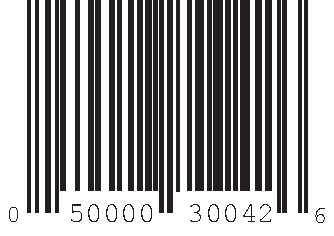
\includegraphics[width=2in]{images/UPCcode.pdf}}{}
\ifthenelse{\boolean{xhtml}}
{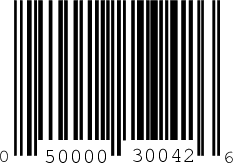
\includegraphics{images/UPCcode.png}}
}
\end{center}
\caption{A UPC code}
\label{groups_figure_3}
\end{figure}

\item
It is often useful to use an inner product notation for this type of error detection scheme; hence, we will use the notion
\[
(d_1, d_2, \ldots, d_k ) \cdot (w_1, w_2, \ldots, w_k ) \equiv 0 \pmod{ n }
\]
to mean
\[
d_1 w_1 +  d_2 w_2 + \cdots +  d_k w_k  \equiv 0  \pmod{ n}.
\]

Suppose that $(d_1, d_2, \ldots, d_k ) \cdot (w_1, w_2, \ldots, w_k ) \equiv 0 \pmod{ n}$ is an error detection scheme for the $k$-digit identification number $d_1 d_2 \cdots d_k$, where $0 \leq d_i < n$.  Prove that all single-digit errors are detected if and only if $\gcd( w_i, n ) = 1$ for  $1 \leq i \leq k$. 

\item
Let $(d_1, d_2, \ldots, d_k ) \cdot (w_1, w_2, \ldots, w_k ) \equiv 0 \pmod{ n}$ be an error detection scheme for the $k$-digit identification number $d_1 d_2 \cdots d_k$, where $0 \leq d_i < n$.  Prove that all transposition errors of two digits $d_i$ and $d_j$ are detected if and only if $\gcd( w_i - w_j, n ) = 1$ for $i$ and  $j$ between 1 and $k$. 

\item
\textbf{ISBN Codes.} 
Every book has an International Standard Book Number\index{International standard book number} (ISBN) code.  This is a 10-digit code indicating the book's publisher and title.  The tenth digit is a check digit satisfying 
\[
(d_1, d_2, \ldots, d_{10} ) \cdot (10, 9, \ldots, 1 )  \equiv 0 \pmod{11}.
\]
One problem is that $d_{10}$ might have to be a 10 to make the inner product zero; in this case, 11 digits would be  needed to make this scheme work.  Therefore, the character X is used for the eleventh digit.  So ISBN 3-540-96035-X is a valid ISBN code. 
\begin{enumerate}
 
 \item
Is ISBN 0-534-91500-0 a valid ISBN code?  What about ISBN 0-534-91700-0 and ISBN 0-534-19500-0? 
 
 \item
Does this method detect all single-digit errors?  What about all transposition errors? 
 
 \item
How many different ISBN codes are there?
 
 \item
Write a computer program that will calculate the check digit for the first nine digits of an ISBN code. 
 
 \item
A publisher has houses in Germany and the United States.  Its German prefix is 3-540.  If its United States prefix will be 0-\textit{abc}, find \textit{abc} such that the rest of the ISBN code will be the same for a book printed in Germany and in the United States. Under the ISBN coding method the first digit identifies the language; German is  3 and English is  0.  The next group of numbers identifies the publisher, and the last group identifies the specific book. 
 
\end{enumerate}
 
\end{enumerate}
}
 
 
 
\subsection*{References and Suggested Readings} % references checked and updated - TWJ 6/22/2010
 
 
{\small
References [2] and [3] show  how group theory can be used in error
detection schemes.  Other sources cover more advanced
topics in group theory. 
\begin{itemize}
 
\item[\textbf{[1]}]  %%Reference updated - TWJ 6/22/2010
Burnside, W. \textit{Theory of Groups of Finite Order}. 2nd ed. Cambridge
University Press, Cambridge, 1911; Dover, New York, 1953.  A classic.  Also available at books.google.com.
 
\item[\textbf{[2]}]
Gallian, J. A. and Winters, S. ``Modular Arithmetic in the
Marketplace,'' \textit{The American Mathematical Monthly} \textbf{
95}(1988): 548--51. 
 
\item[\textbf{[3]}]  %%Reference updated - TWJ 6/22/2010
Gallian, J. A. 
\textit{Contemporary Abstract Algebra}. 7th ed. Brooks/Cole, Belmont, CA, 2009. 
 
\item[\textbf{[4]}]   %%Reference updated - TWJ 6/22/2010
Hall, M. \textit{Theory of Groups}. 2nd ed. American Mathematical Society, Providence, 1959.

 
\item[\textbf{[5]}] %%Reference updated - TWJ 6/22/2010
Kurosh, A. E. \textit{The Theory of Groups}, vols. I and II. American Mathematical Society, Providence, 1979. 
 
 
%%  The following two books are out of print and probably not readily available - TWJ 6/22/2010 

%\item[\textbf{[6]}]  
%MacDonald, I. D. \textit{The Theory of Groups}. Krieger, London, 1988.
% 
%\item[\textbf{[7]}]
%Rose, J. S. \textit{A Course on Group Theory}. Cambridge University
%Press, Cambridge, 1978.
 
 
\item[\textbf{[6]}] %%Reference updated 6/22/2010 - TWJ
Rotman, J. J. \textit{An Introduction to the Theory of
Groups}. 4th ed. Springer, New York, 1995.
 
\end{itemize}
}
 
\sagesection
   %Groups
%%%%(c)
%%%%(c)  This file is a portion of the source for the textbook
%%%%(c)
%%%%(c)    Abstract Algebra: Theory and Applications
%%%%(c)    Copyright 1997 by Thomas W. Judson
%%%%(c)
%%%%(c)  See the file COPYING.txt for copying conditions
%%%%(c)
%%%%(c)
\chap{Cyclic Groups}{cyclic}
 
The groups $\mathbb Z$ and ${\mathbb Z}_n$, which are among the most familiar and easily understood groups, are both examples of what are called cyclic groups.  In this chapter we will study the properties of cyclic groups and cyclic subgroups, which play a fundamental part in the classification of all abelian groups. 


\section{Cyclic Subgroups}

Often a subgroup will depend entirely on a single element of the group; that is, knowing that particular element will allow us to compute any other element in the subgroup. 

\begin{example}{Cyclic_Z3}
Suppose that we consider $3 \in {\mathbb Z}$ and look at all multiples (both positive and negative) of 3.  As a set, this is 
\[
3 {\mathbb Z} = \{ \ldots, -3, 0, 3, 6, \ldots \}.
\]
It is easy to see that $3 {\mathbb Z}$ is a subgroup of the integers.  This subgroup is completely determined by the element 3 since we can obtain all of the other elements of the group by taking multiples of 3.  Every element in the subgroup is ``generated'' by 3. 
\end{example}

\begin{example}{Cyclic_2^n}
If $H = \{ 2^n : n \in {\mathbb Z} \}$, then $H$ is a subgroup of the multiplicative group of nonzero rational numbers, ${\mathbb Q}^*$.  If $a = 2^m$ and $b = 2^n$ are in $H$, then $ab^{-1} = 2^m 2^{-n} = 2^{m-n}$ is also in $H$.  By Proposition~\ref{groups:subgroup_prop}, $H$ is a subgroup of ${\mathbb Q}^*$ determined by the element 2. 
\end{example}

\begin{theorem}\label{cyclic:cyclicsubgroup}
Let $G$ be a group and $a$ be any element in $G$.  Then the set
\[
\langle a \rangle  = \{ a^k : k \in {\mathbb Z} \}\label{generatedby}
\]
is a subgroup of $G$.  Furthermore, $\langle a \rangle$ is the smallest subgroup of $G$ that contains~$a$. 
\end{theorem}
 
 
\begin{proof}
The identity is in $\langle a \rangle $ since $a^0 = e$. If $g$ and
$h$ are any two elements in $\langle a \rangle $, then by the
definition of $\langle a \rangle$ we can write $g = a^m$ and $h = a^n$
for some integers $m$ and $n$. So $gh = a^m a^n = a^{m+n}$ is again in
$\langle a \rangle $. Finally, if $g = a^n$ in $\langle a \rangle $,
then the inverse $g^{-1} = a^{-n}$ is also in $\langle a \rangle $.
Clearly, any subgroup $H$ of $G$ containing $a$ must contain all the
powers of $a$ by closure; hence, $H$ contains $\langle a \rangle $.
Therefore, $\langle a \rangle $ is the smallest subgroup of $G$
containing $a$. 
\end{proof}
 
 
\medskip
 
 
\noindent \textbf{Remark.}
If we are using the ``+'' notation, as in the case of the integers under
addition, we write $\langle a \rangle  = \{ na : n \in {\mathbb Z} \}$.
 
 
\medskip
 
 
For $a \in G$, we call $\langle a \rangle $ the \boldemph{cyclic
subgroup}\index{Subgroup!cyclic} generated by $a$. If $G$ contains
some element $a$ such that $G = \langle a \rangle $, then $G$ is a
\boldemph{cyclic group}\index{Group!cyclic}. In this case $a$ is a \boldemph{
generator}\index{Generator of a cyclic subgroup} of $G$.  If $a$ is an
element of a group $G$, we define the \boldemph{order}\index{Element!order
of} of $a$ to be the smallest positive integer $n$ such that $a^n= e$,
and we write $|a| = n$\label{noteelementorder}. If there is no such
integer $n$, we say that the order of $a$ is infinite and  write $|a|
= \infty$ to denote the order of $a$.
 
 
\begin{example}{Cyclic_Z6}
Notice that a cyclic group can have more than a single
generator. Both 1 and 5 generate ${\mathbb Z}_6$; hence, ${\mathbb Z}_6$ is
a cyclic group. Not every element in a cyclic group is necessarily a
generator of the group. The order of $2 \in {\mathbb Z}_6$ is 3. The
cyclic subgroup generated by 2 is $\langle 2 \rangle  = \{ 0, 2, 4
\}$.  
\end{example}
 
 
The groups ${\mathbb Z}$ and ${\mathbb Z}_n$ are cyclic groups. The elements
1 and $-1$ are generators for ${\mathbb Z}$.  We can certainly generate
${\mathbb Z}_n$ with 1 although there may be other generators of ${\mathbb
Z}_n$, as in the case of ${\mathbb Z}_6$. 
 
 
\begin{example}{Cyclic_U9}
The group of units, $U(9)$, in ${\mathbb Z}_9$ is a cyclic group.  As a
set, $U(9)$ is $\{ 1, 2, 4, 5, 7, 8  \}$. The element 2 is a generator
for $U(9)$ since 
\begin{align*}
2^1 & = 2 \qquad 2^2 = 4 \\
2^3 & = 8 \qquad 2^4 = 7 \\
2^5 & =  5 \qquad 2^6 = 1.
\end{align*}
\end{example}
 
 
\begin{example}{Not_Cyclic_S3}
Not every group is a cyclic group.  Consider the symmetry group of an
equilateral triangle $S_3$.  The multiplication table for this group
is Table~\ref{S3_table}. The subgroups of $S_3$ are shown in
Figure~\ref{subgrpsS3}.  Notice that every subgroup is cyclic;
however, no single element generates the entire group.
\hspace*{1in}
\end{example}


\begin{figure}[htb] %Replaced figure with tikz figure - TWJ 5/6/2010
\begin{center}
\tikzpreface{cyclic_s3_subgroups}
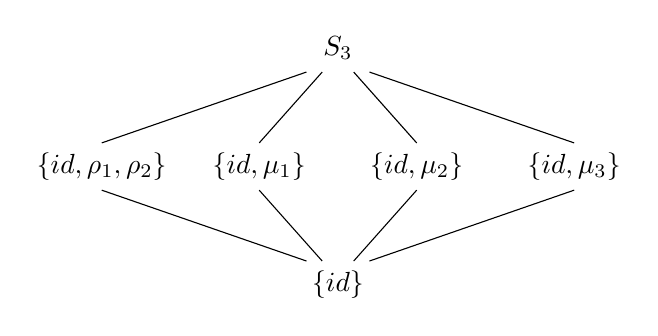
\begin{tikzpicture}[scale=1]

\draw  (0,0.3) -- (2.6,1.2);
\draw  (2,0.3) -- (2.8,1.2);
\draw  (4,0.3) -- (3.2,1.2);
\draw  (6,0.3) -- (3.4,1.2);

\draw  (0,-0.3) -- (2.6,-1.2);
\draw  (2,-0.3) -- (2.8,-1.2);
\draw  (4,-0.3) -- (3.2,-1.2);
\draw  (6,-0.3) -- (3.4,-1.2);

\node at (0, 0) {$\{  id, \rho_1, \rho_2\}$};
\node at (2, 0) {$\{  id, \mu_1\}$};
\node at (4, 0) {$\{  id, \mu_2 \}$};
\node at (6, 0) {$\{  id, \mu_3 \}$};
\node at (3, 1.5) {$S_3$};
\node at (3,-1.5) {$\{ id \}$};
\end{tikzpicture}
\end{center}
\caption{Subgroups of $S_3$}
\label{subgrpsS3}
\end{figure}
 
 
\begin{theorem}\label{cyclic:cyclicabelian}
Every cyclic group is abelian.
\end{theorem}
 
 
\begin{proof}
Let $G$ be a cyclic group and $a \in G$ be a generator for $G$. If
$g$ and $h$ are in $G$, then they can be written as powers of $a$,
say $g = a^r$ and $h = a^s$. Since
\[
g  h = a^r a^s = a^{r+s} = a^{s+r} = a^s a^r = h g,
\]
$G$ is abelian.
\end{proof}
 
 
 
\subsection*{Subgroups of Cyclic Groups}
 
 
We can ask some interesting questions about cyclic subgroups of a
group and subgroups of a cyclic group.  If $G$ is a group, which
subgroups of $G$ are cyclic? If $G$ is a cyclic group, what type of
subgroups does $G$ possess? 
 
 
 
\begin{theorem}\label{cyclic:subgroups}
Every subgroup of a cyclic group is cyclic.
\end{theorem}
 
 
\begin{proof}
The main tools used in this proof are the division algorithm and the
Principle of Well-Ordering. Let $G$ be a cyclic group generated by $a$
and suppose that $H$ is a subgroup of $G$. If $H = \{ e \}$, then
trivially $H$ is cyclic. Suppose that $H$ contains some other element
$g$ distinct from the identity. Then $g$ can be written as
$a^n$ for some integer $n$. We can assume that $n > 0$. Let $m$ be the
smallest natural number such that $a^m \in H$. Such an $m$ exists by
the Principle of Well-Ordering.
 
 
We claim that $h = a^m$ is a generator for $H$.  We must show that
every $h' \in H$ can be written as a power of $h$. Since $h' \in H$
and $H$ is a subgroup of $G$, $h' = a^k$ for some positive integer
$k$. Using the division algorithm, we can find numbers $q$ and $r$
such that $k = mq +r$ where $0 \leq r < m$; hence,
\[
a^k = a^{mq +r} = (a^m)^q a^r = h^q a^r.
\]
So $a^r = a^k h^{-q}$. Since $a^k$ and $h^{-q}$ are in $H$, $a^r$ must
also be in $H$.  However, $m$ was the smallest positive number such that
$a^m$ was in $H$; consequently, $r=0$ and so $k=mq$. Therefore, 
\[
h' = a^k = a^{mq} =  h^q
\]
and $H$ is generated by $h$.
\end{proof}
 
 
\begin{corollary}
The subgroups of ${\mathbb Z}$ are exactly $n{\mathbb Z}$ for $n = 0, 1, 2,
\ldots$. 
\end{corollary}
 
 
\begin{proposition}\label{Cyclic_subgrp_order}
Let $G$ be a cyclic group of order $n$ and suppose that $a$ is a
generator for  $G$. Then $a^k=e$ if and only if $n$ divides $k$.
\end{proposition}
 
 
\begin{proof}
First suppose that $a^k=e$. By the division algorithm, $k = nq + r$
where $0 \leq r < n$; hence, 
\[
e = a^k = a^{nq + r} = a^{nq} a^r = e a^r = a^r.
\]
Since the smallest positive integer $m$ such that $a^m = e$ is $n$, $r
= 0$.
 
 
Conversely, if $n$ divides $k$, then $k=ns$ for some integer $s$.
Consequently, 
\[
a^k = a^{ns} = (a^n)^s = e^s = e.
\]
\end{proof}
 
 
\begin{theorem}\label{cyclic:orders}
Let $G$ be a cyclic group of order $n$ and suppose that $a \in G$ is a
generator of the group.  If $b = a^k$, then the order of $b$ is $n
/d$, where $d = \gcd(k,n)$. 
\end{theorem}
 
 
\begin{proof}
We wish to find the smallest integer $m$ such that $e = b^m = a^{km}$.
By Proposition~\ref{Cyclic_subgrp_order}, this is the smallest integer $m$ such that
$n$ divides $km$ or, equivalently, $n/d$ divides $m(k/d)$.  Since $d$ is
the greatest common divisor of $n$ and $k$, $n/d$ and $k/d$ are
relatively prime. Hence, for $n/d$ to divide $m(k/d)$ it must divide
$m$.  The smallest such $m$ is $n/d$. 
\end{proof}
 
 
\begin{corollary}\label{cyclic:modngenerators}
The generators of ${\mathbb Z}_n$ are the integers $r$ such that $1 \leq
r < n$ and $\gcd(r,n) =  1$. 
\end{corollary}
 
 
\begin{example}{Cyclic_Z16}
Let us examine the group ${\mathbb Z}_{16}$.  The numbers 1, 3, 5, 7, 9,
11, 13, and 15 are the elements of ${\mathbb Z}_{16}$ that are relatively
prime to 16.  Each of these elements generates ${\mathbb Z}_{16}$. For
example, 
\begin{align*}
1 \cdot 9  & =  9  &  2 \cdot 9  & = 2  & 3 \cdot 9  & = 11 \\
4 \cdot 9  & =  4  &  5 \cdot 9  & = 13 & 	6 \cdot 9 & = 6  \\
7 \cdot 9  & =  15 & 8 \cdot 9  & = 8  & 	9 \cdot 9 &  = 1  \\
10 \cdot 9 & =  10 & 11 \cdot 9 & = 3  & 12 \cdot 9 &  = 12 \\
13 \cdot 9 & =  5 & 14 \cdot 9 & = 14 &  	15 \cdot 9 & = 7.
\end{align*}
\end{example}
 
 
%\section{The Group ${\mathbb C}^\ast$}

\section{Multiplicative Group of Complex Numbers}
 
 
The \boldemph{complex numbers} are defined as
\[
{\mathbb C} = \{ a + bi : a, b \in {\mathbb R} \},
\]
where $i^2 = -1$.  If $z=a+bi$, then $a$ is the \boldemph{real part} of $z$
and $b$ is the \boldemph{imaginary part} of $z$. 
 
 
To add two complex numbers $z=a+bi$ and $w= c+di$, we just
add the corresponding real and imaginary parts:
\[
z+w=(a + bi ) + (c + di)  =  (a+c) + (b+d)i.
\]
Remembering that $i^2 = -1$,  we multiply complex numbers just like
polynomials. The product of $z$ and $w$ is 
\[
(a + bi )(c + di)  =   ac + bdi^2 + adi + bci =  (ac -bd) +
(ad + bc)i.
\]
 
 
Every nonzero complex number $z = a +bi$ has a multiplicative inverse;
that is, there exists a $z^{-1} \in {\mathbb C}^\ast$ such that $z z^{-1}
= z^{-1} z = 1$. If $z = a + bi$, then 
\[
z^{-1} = \frac{a-bi}{ a^2 + b^2  }.
\]
The \boldemph{complex conjugate}\index{Conjugate, complex} of a complex
number $z = a +bi$ is defined to be $\overline{z} = a-bi$.  The \boldemph{
absolute value} or \boldemph{modulus} of  $z = a +bi$  is $|z| =
\sqrt{a^2+b^2}$.  
 
 
\begin{example}{complex_add}
Let $z = 2 + 3i$ and $w = 1-2i$. Then
\[
z + w = (2 + 3i)+( 1-2i ) = 3 +i
\]
and
\[
z  w = (2 + 3i)( 1-2i ) = 8-i.
\]
Also,
\begin{align*}
z^{-1} & = \frac{2}{13} - \frac{3}{13}i \\
|z| & = \sqrt{13} \\
\overline{z} & = 2-3i.
\end{align*}
\end{example}
 
\begin{figure}[hbt]  %Replaced figure with tikz figure - TWJ 5/6/2010
\begin{center}
\tikzpreface{cyclic_complex_rectangular}
\begin{tikzpicture}[scale=0.5]

\draw [->]  (0,-5) -- (0,5);
\draw  [->] (-8,0) -- (8,0);
\node [right] at (0,5) {$y$};
\node [below] at (8,0) {$x$};
\node [below] at (0.5,0) {$0$};

\filldraw[fill=black, draw=black] (2,3) circle (0.05cm);
\node [right] at (2,3) {$z_1 = 2 + 3i$};

\filldraw[fill=black, draw=black] (-3,2) circle (0.05cm);
\node [left] at (-3, 2) {$z_3 = -3 + 2i$};

\filldraw[fill=black, draw=black] (1,-2) circle (0.05cm);
\node [right] at (1, -2) {$z_2 = 1 -  2i$};

\end{tikzpicture}
\end{center}
\caption{Rectangular coordinates of a complex number}
\label{rectcoord}
\end{figure}
 
 
There are several ways of graphically representing complex numbers. We
can represent a complex number $z = a +bi$ as an ordered pair on the
$xy$ plane where $a$ is the $x$ (or real) coordinate and $b$ is the $y$
(or imaginary) coordinate. This is called the \boldemph{rectangular} or
\boldemph{Cartesian} representation. The rectangular representations of
$z_1 = 2 + 3i$, $z_2 = 1 - 2i$, and $z_3 = - 3 + 2i$ are depicted in
Figure~\ref{rectcoord}.
 
 
\begin{figure}[htb]
\begin{center}
\tikzpreface{cyclic_complex_polar}
\begin{tikzpicture}[scale=0.5] %Replaced figure with tikz figure - TWJ 5/6/2010

\draw [->]  (0,-5) -- (0,5);
\draw  [->] (-8,0) -- (8,0);
\node [right] at (0,5) {$y$};
\node [below] at (8,0) {$x$};
\node [below] at (0.5,0) {$0$};

\draw (0,0) -- (35:6);
\draw (2,0) arc (0:35:2);

\filldraw[fill=black, draw=black] (35:6) circle (0.05cm);
\node [right] at (35:6) {$a + bi$};
\node [above] at (35:3) {$r$};
\node [right] at (17:2) {$\theta$};

\end{tikzpicture}

\end{center}
\caption{Polar coordinates of a complex number}
\label{polarcoord}
\end{figure}
 
 
Nonzero complex numbers can also be represented using \boldemph{polar
coordinates}.  To specify  any nonzero point on the plane, it suffices
to give an angle $\theta$ from the positive $x$ axis in the
counterclockwise direction and a distance $r$ from the origin, as in 
Figure~\ref{polarcoord}. We can see that 
\[
z = a + bi = r( \cos \theta + i \sin \theta).
\]
Hence,
\[
r = |z| = \sqrt{a^2+b^2}
\]
and
\begin{align*}
a & = r \cos \theta \\
b & = r \sin \theta.
\end{align*}
We sometimes abbreviate $r( \cos \theta + i \sin \theta)$ as $r \cis
\theta$\label{cosisin}.  To assure that the representation of $z$ is 
well-defined, we also require that $0^{\circ} \leq \theta <
360^{\circ}$.  If the measurement is in radians, then $0 \leq \theta <
2 \pi$. 
 
\begin{example}{polar}
Suppose that $z = 2 \cis  60^{\circ}$. Then
\[
a  =  2 \cos 60^{\circ}  =   1
\]
and
\[
b  =  2 \sin 60^{\circ}  =  \sqrt{3}.
\]
Hence, the rectangular representation is $z = 1+\sqrt{3}\, i$.
 
 
Conversely, if we are given a rectangular representation of a complex
number, it is often useful to know the number's polar representation.
If $z = 3 \sqrt{2} - 3 \sqrt{2}\, i$, then 
\[
r = \sqrt{a^2 + b^2} = \sqrt{36 } = 6
\]
and
\[
\theta = \arctan \left( \frac{b}{a} \right) = \arctan( - 1) =
315^{\circ},
\]
so $3 \sqrt{2} - 3 \sqrt{2}\, i=6 \cis  315^{\circ}$.
\end{example}
 
 
The polar representation of a complex number makes it easy to find
products and powers of complex numbers.  The proof of the following
proposition is straightforward and is left as an exercise.
 
 
\begin{proposition}\label{polar_mult}
Let $z = r \cis \theta$ and $w = s \cis \phi$
be two nonzero complex numbers. Then 
\[
zw = r s \cis( \theta + \phi).
\]
\end{proposition}
 
 
\begin{example}{polar_mult}
If $z =  3 \cis( \pi / 3 )$ and $w = 2 \cis(\pi / 6 )$, then $zw = 6
\cis( \pi / 2 ) = 6i$.  
\end{example}
 
 
\begin{theorem}[DeMoivre]\index{DeMoivre's Theorem}
Let $z = r \cis  \theta$ be a nonzero complex number. Then 
\[
[r \cis \theta  ]^n
=
r^n \cis( n \theta)
\]
for $n = 1, 2, \ldots$.
\end{theorem}
 
 
\begin{proof}
We will use induction on $n$. For $n = 1$ the theorem is trivial.
Assume that the theorem is true for all $k$ such that $1  \leq k \leq
n$. Then 
\begin{align*}
z^{n+1} & = z^n z \\
& =
r^n( \cos  n \theta + i \sin n \theta ) r( \cos \theta + i
\sin \theta ) \\
& =
r^{n+1} [( \cos n \theta \cos \theta - \sin n \theta \sin
\theta )
 + i ( \sin n \theta \cos \theta + \cos n \theta \sin \theta
)] \\
& =
r^{n+1} [ \cos( n \theta + \theta) + i \sin( n \theta +
\theta) ] \\
& =
r^{n+1} [ \cos( n +1) \theta + i \sin( n+1) \theta  ].
\end{align*}
\end{proof}
 
 
\begin{example}{DeMoivre}
Suppose that $z= 1+i$ and we wish to compute $z^{10}$. Rather than
computing $(1+i)^{10}$ directly, it is much easier to switch to polar
coordinates and calculate $z^{10}$ using DeMoivre's Theorem:
\begin{align*}
z^{10}
& =
(1+i)^{10} \\
& =
\left( \sqrt{2} \cis \left( \frac{\pi }{4} \right)
\right)^{10} \\
& =
( \sqrt{2}\, )^{10} \cis \left( \frac{5\pi }{2} \right)
\\
& =
32  \cis \left( \frac{\pi }{2} \right) \\
& = 32i.
\end{align*}
\end{example}
 
 
\subsection*{The Circle Group and the Roots of Unity }
 
 
The multiplicative group of the complex numbers, ${\mathbb C}^*$,
possesses some interesting subgroups.  Whereas ${\mathbb Q}^*$ and ${\mathbb
R}^*$ have no interesting subgroups of finite order, ${\mathbb C}^*$ has 
many. We first consider the \boldemph{circle group}\index{Group!circle}, 
\[
{\mathbb T}\label{notecirclegroup} = \{ z \in {\mathbb C} : |z| = 1 \}.
\]
The following proposition is a direct result of Proposition~\ref{polar_mult}.
 
 
\begin{proposition}
The circle group is a subgroup of  ${\mathbb C}^*$.
\end{proposition}
 
 
Although the circle group has infinite order, it has many interesting 
finite subgroups. Suppose that $H = \{ 1, -1, i, -i \}$. Then $H$ is a
subgroup of the circle group. Also, $1$, $-1$, $i$, and $-i$ are
exactly those complex numbers that satisfy the equation $z^4=1$. 
The complex numbers satisfying the equation $z^n=1$ are called
the \boldemph{nth roots of unity}\index{$n$th root of unity}. 
 
 
\begin{theorem}
If $z^n = 1$, then the $n$th roots of unity are
\[
z = \cis\left( \frac{2 k \pi}{n } \right),
\]
where $k = 0, 1, \ldots, n-1$. Furthermore, the $n$th roots of unity
form a cyclic subgroup of\/ ${\mathbb T}$ of order $n$. 
\end{theorem}
 
 
\begin{proof}
By DeMoivre's Theorem,
\[
z^n = \cis \left( n \frac{2 k \pi}{n } \right) =
\cis( 2 k \pi ) = 1.
\]
The $z$'s are distinct since the numbers $2 k \pi /n$ are all
distinct and are greater than or equal to 0 but less than $2 \pi$.
The fact that these are all of the roots of the equation $z^n=1$
follows from from Corollary~\ref{poly:zeros_corollary}, which
states that a polynomial of degree $n$ can have at most $n$ roots.  We
will leave the proof that the $n$th roots of unity form a cyclic
subgroup of ${\mathbb T}$ as an exercise.
\end{proof}
 
 
\medskip
 
 
A generator for the group of the $n$th roots of unity is called a
\boldemph{primitive nth root of unity}\index{Primitive $n$th root of
unity}. 
 
 
\begin{example}{roots_unity}
The 8th roots of unity can be represented as
eight equally spaced points on the unit circle (Figure~\ref{rtsunity}).  The
primitive 8th roots of unity are
\begin{align*}
\omega & = \frac{\sqrt{2}}{2}  + \frac{\sqrt{2}}{2} i \\
\omega^3 & = -\frac{\sqrt{2}}{2}  + \frac{\sqrt{2}}{2} i \\
\omega^5 & = -\frac{\sqrt{2}}{2}  - \frac{\sqrt{2}}{2} i \\
\omega^7 & = \frac{\sqrt{2}}{2}  - \frac{\sqrt{2}}{2}i. 
\end{align*}
\end{example}
 
 

\begin{figure}[hbt]
\begin{center}
\tikzpreface{cyclic_roots_unity}
\begin{tikzpicture}[scale=1.65] %Replaced figure with tikz figure - TWJ 5/6/2010

\draw [->]  (0,-1.5) -- (0,1.5);
\draw  [->] (-1.75,0) -- (1.75,0);
\node [right] at (0,1.5) {$y$};
\node [below] at (1.75,0) {$x$};
\node [below] at (0.1,0) {$0$};

\draw (0,0) circle (1);

\filldraw[fill=black, draw=black] (0:1) circle (0.03);
\filldraw[fill=black, draw=black] (45:1) circle (0.03);
\filldraw[fill=black, draw=black] (90:1) circle (0.03);
\filldraw[fill=black, draw=black] (135:1) circle (0.03);
\filldraw[fill=black, draw=black] (180:1) circle (0.03);
\filldraw[fill=black, draw=black] (225:1) circle (0.03);
\filldraw[fill=black, draw=black] (270:1) circle (0.03);
\filldraw[fill=black, draw=black] (315:1) circle (0.03);


\node [right] at (1,-0.15) {1};
\node [right] at (45:1) {$\omega$};
\node [left] at (0,1.15) {$i$};
\node [left] at (135:1) {$\omega^3$};
\node [left] at (-1,-0.15) {$-1$};
\node [left] at (225:1) {$\omega^5$};
\node [left] at (0,-1.15) {$-i$};
\node [right] at (315:1) {$\omega^7$};

\end{tikzpicture}

\end{center}
\caption{8th roots of unity}
\label{rtsunity}
\end{figure}
 
 
 
 
\section[The Method of Repeated Squares]{The Method of Repeated
Squares\protect\footnotemark}\index{Repeated squares} 
\footnotetext{The results in this section are needed only in
Chapter~\ref{crypt}.}   
 
 
Computing large powers can be very time-consuming. Just as anyone can
compute $2^2$ or $2^8$, everyone knows how to compute
\[
2^{2^{1000000} }.
\]
However, such numbers are so large that we do not want to attempt the
calculations; moreover, past a certain point the computations would not
be feasible even if we had every computer in the world at our
disposal. Even 
writing down the decimal representation of a very large number may not
be reasonable. It could be thousands or even millions of digits long.
However, if we could compute something like $2^{37398332 } \pmod{
46389}$, we could very easily write the result down since it would be a
number between 0 and 46,388. If we want to compute powers modulo $n$
quickly and efficiently, we will have to be clever. 
 
 
The first thing to notice is that any number $a$ can be written as the
sum of distinct powers of 2; that is, we can write
\[
a = 2^{k_1} + 2^{k_2} + \cdots + 2^{k_n},
\]
where $k_1 < k_2 < \cdots < k_n$.  This is just the binary
representation of $a$. For example, the binary representation of 57 is
111001, since we can write $57 = 2^0 + 2^3 + 2^4 + 2^5$.
 
 
The laws of exponents still work in ${\mathbb Z}_n$; that is, if $b
\equiv a^x \pmod{ n}$ and $c \equiv a^y \pmod{ n}$, then $bc \equiv
a^{x+y} \pmod{ n}$. We can compute $a^{2^k} \pmod{ n}$ in $k$
multiplications by computing 
\begin{gather*}
a^{2^0} \pmod{ n} \\
a^{2^1} \pmod{ n }\\
\vdots \\
a^{2^k} \pmod{ n}.
\end{gather*}
Each step involves squaring the answer obtained in the previous step,
dividing by $n$, and taking the remainder.
 
 
\begin{example}{repeated_squares}
We will compute $271^{321} \pmod{ 481}$. Notice that
\[
321 = 2^0 +2^6 + 2^8;
\]
hence, computing $271^{ 321} \pmod{ 481}$ is the same as computing
\[
271^{ 2^0 +2^6 + 2^8 } \equiv 271^{ 2^0 } \cdot 271^{2^6 } \cdot 271^{ 2^8 } \pmod{ 481}.
\]
So it will suffice to compute $271^{ 2^i } \pmod{ 481}$ where $i = 0,
6, 8$. It is very easy to see that 
\[
271^{ 2^1}  = \mbox{73,441} 
 \equiv 329 \pmod{ 481}.
\]
We can square this result to obtain a value for $271^{ 2^2} \pmod{481}$: 
\begin{align*}
271^{ 2^2}  & \equiv (271^{ 2^1})^2 \pmod{ 481} \\ 
& \equiv (329)^2 \pmod{ 481} \\
& \equiv \mbox{108,241} \pmod{ 481} \\
& \equiv 16 \pmod{ 481}.
\end{align*}
We are using the fact that $(a^{2^n})^2  \equiv a^{2 \cdot 2^n} \equiv
a^{ 2^{n+1} } \pmod{ n}$. Continuing, we can calculate
\[
271^{ 2^6 } \equiv 419 \pmod{ 481}
\]
and
\[
271^{ 2^8 }  \equiv 16 \pmod{ 481}.
\]
Therefore,
\begin{align*}
271^{ 321}
& \equiv 271^{ 2^0 +2^6 + 2^8 } \pmod{ 481} \\
& \equiv 271^{ 2^0 } \cdot 271^{ 2^6 } \cdot 271^{ 2^8 } \pmod{ 481} \\
& \equiv 271 \cdot 419 \cdot 16 \pmod{ 481} \\
& \equiv \mbox{1,816,784} \pmod{ 481} \\
& \equiv 47 \pmod{ 481}.
\end{align*}
\end{example}

%Reformatted example.  TWJ 2/5/2013
 
 
The method of repeated squares will prove to be a very useful tool
when we explore  RSA cryptography  in Chapter~\ref{crypt}. To encode and decode
messages in a reasonable manner under this scheme, it is necessary to
be able to quickly compute large powers of integers mod $n$.
 
 
\markright{EXERCISES}
\section*{Exercises}
\exrule
 
 
 
 
{\small
\begin{enumerate}
 
 
\item
Prove or disprove each of the following statements.
\begin{enumerate}
 
 \item
$U(8)$ is cyclic.
 
 \item
All of the generators of ${\mathbb Z}_{60}$ are prime.
 
 \item
${\mathbb Q}$ is cyclic.
 
 \item
If every proper subgroup of a group $G$ is cyclic, then $G$ is a cyclic
group. 
%Changed the problem to read proper subgroup.  Suggested by A. Glesser. - TWJ 2/1/2012
 
 \item
A group with a finite number of subgroups is finite.
 
\end{enumerate}
 
  
\item
Find the order of each of the following elements.
\begin{multicols}{3}
\begin{enumerate}

\item
$5 \in {\mathbb Z}_{12}$

\item
$\sqrt{3} \in {\mathbb R}$
 
\item
$\sqrt{3} \in {\mathbb R}^\ast$
 
\item
$-i \in {\mathbb C}^\ast$

\item
72 in ${\mathbb Z}_{240}$
 
\item
312 in ${\mathbb Z}_{471}$
 
 \end{enumerate}
 \end{multicols}
  
\item
List all of the elements in each of the following subgroups.
\begin{enumerate}
 
 \item
The subgroup of ${\mathbb Z}$ generated by 7
 
 \item
The subgroup of ${\mathbb Z}_{24}$ generated by 15
 
 \item
All subgroups of ${\mathbb Z}_{12}$
 
 \item
All subgroups of ${\mathbb Z}_{60}$
 
 \item
All subgroups of ${\mathbb Z}_{13}$
 
 \item
All subgroups of ${\mathbb Z}_{48}$
 
 \item
The subgroup generated by 3  in $U(20)$
 
 \item
The subgroup generated by 5 in $U(18)$  %Changed 6 to 5 so that the problem would make sense.  Suggested by Aziz Azizov - TWJ 12/9/2010
 
 \item
The subgroup of ${\mathbb R}^\ast$ generated by 7
 
 \item
The subgroup of ${\mathbb C}^\ast$ generated by $i$ where $i^2 = -1$
 
 \item
The subgroup of ${\mathbb C}^\ast$ generated by $2i$
 
 \item
The subgroup of ${\mathbb C}^\ast$ generated by $(1 + i) / \sqrt{2}$
 
 \item
The subgroup of ${\mathbb C}^\ast$ generated by $(1 + \sqrt{3}\, i) / 2$
 
\end{enumerate}
 
 
\item
Find the subgroups of $GL_2( {\mathbb R })$ generated by each of the
following matrices. 
\begin{multicols}{3}
\begin{enumerate}
 
\item
$\displaystyle
\begin{pmatrix}
0 & 1 \\
-1 & 0
\end{pmatrix}
$

\item
$\displaystyle
\begin{pmatrix}
0 & 1/3 \\
3 & 0
\end{pmatrix}
$

\item
$\displaystyle
\begin{pmatrix}
1 & -1 \\
1 & 0
\end{pmatrix}
$

\item
$\displaystyle
\begin{pmatrix}
1 & -1 \\
0 & 1
\end{pmatrix}
$

\item
$\displaystyle
\begin{pmatrix}
1 & -1 \\
-1 & 0
\end{pmatrix}
$
 
\item
$\displaystyle
\begin{pmatrix}
\sqrt{3}/ 2 & 1/2 \\
-1/2 & \sqrt{3}/2
\end{pmatrix}
$

 \end{enumerate}
\end{multicols}

 

\item		  %%%%%%%%%%%%%%%%%%%%%%%%
Find the order of every element in ${\mathbb Z}_{18}$.
 
 
\item
Find the order of every element in the symmetry group of the square,
$D_4$.
 
 
\item
What are all of the cyclic subgroups of the quaternion group, $Q_8$? 
 
 
\item
List all of the cyclic subgroups of $U(30)$.
 
 
\item
List every generator of each subgroup of order 8 in ${\mathbb
Z}_{32}$.
 
% 2010/05/10 R Beezer: Added explanation of the * on sets
\item
Find all elements of finite order in each of the following groups. Here the ``$\ast$'' indicates the set with zero removed.
\begin{multicols}{3}
\begin{enumerate}
 
 \item
${\mathbb Z}$
 
 \item
${\mathbb Q}^\ast$
 
 \item
${\mathbb R}^\ast$
 
\end{enumerate}
 \end{multicols}
 
\item
If $a^{24} =e$ in a group $G$, what are the possible orders of $a$? 
 
 
\item
Find a cyclic group with exactly one generator.  Can you find cyclic
groups with exactly two generators?  Four generators?  How about $n$
generators?
 
 
\item
For $n \leq 20$, which groups $U(n)$ are cyclic?  Make a conjecture as
to what is true in general.  Can you prove your conjecture?  
 
 
\item
Let
\[
A=
\begin{pmatrix}
0 & 1 \\
-1 & 0
\end{pmatrix}
\qquad \text{and} \qquad
B=
\begin{pmatrix}
0 & -1 \\
1 & -1
\end{pmatrix}
\]
be elements in $GL_2( {\mathbb R} )$. Show that $A$ and $B$ have finite
orders but $AB$ does not. 
 
 
\item
Evaluate each of the following.
\begin{multicols}{2}
\begin{enumerate}
 
\item
$(3-2i)+ (5i-6)$

 
\item
 $(4-5i)-\overline{(4i -4)}$
 
 \item
$(5-4i)(7+2i)$
 
\item
$(9-i) \overline{(9-i)}$
 
 \item
$i^{45}$

\item
$(1+i)+\overline{(1+i)}$
 
\end{enumerate}
\end{multicols}
 
 
 \item   %%%%%%%%%%%%%%%%%%%%%%%%
Convert the following complex numbers to the form $a + bi$.
\begin{multicols}{2}
\begin{enumerate}

 \item
$2 \cis(\pi / 6 )$

 
 \item
$5 \cis(9\pi/4)$

\item
$3 \cis(\pi)$
 
 \item
$\cis(7\pi/4) /2$
 
\end{enumerate}
\end{multicols}


\item	  %%%%%%%%%%%%%%%%%%%%%%%%%%%%%%%%
Change the following complex numbers to polar representation.
\begin{multicols}{3}
\begin{enumerate}
 
 \item
$1-i$

 \item
$-5$
 
 \item
$2+2i$
 
 
\item
$\sqrt{3} + i$

 \item
$-3i$

 \item
$2i + 2 \sqrt{3}$
 
\end{enumerate}
\end{multicols}

 
 
\item %%%%%%%%%%%%%%%%%%%%%%%%
Calculate each of the following expressions.
\begin{multicols}{2}
\begin{enumerate}
 
 \item
$(1+i)^{-1}$

 \item
$(1 - i)^{6}$
 
 \item
$(\sqrt{3}+i)^{5}$

 \item
$(-i)^{10}$
 
 \item
$((1-i)/2)^{4}$

 \item
$(-\sqrt{2} - \sqrt{2}\, i)^{12}$
 
 \item
$(-2+2i)^{-5}$
 
\end{enumerate}
\end{multicols}

  
  \item
Prove each of the following statements.
\begin{multicols}{2}
\begin{enumerate}
 
 \item
$|z| = | \overline{z}|$

\item
$z \overline{z} = |z|^2$
 
 \item
$z^{-1} = \overline{z} / |z|^2$

 \item
$|z +w| \leq |z| + |w|$
 
 \item
$|z - w| \geq | |z| - |w||$
 
 \item
$|z w| = |z|  |w|$
 
\end{enumerate}
\end{multicols}


\item
List and graph the 6th roots of unity.  What are the generators of
this group?  What are the primitive 6th roots of unity?
 
 
\item
List and graph the 5th roots of unity.  What are the generators of
this group?  What are the primitive 5th roots of unity? 
 
 
  
\item
Calculate each of the following.
\begin{multicols}{2}
\begin{enumerate}
 
 \item
$292^{3171} \pmod{ 582}$

\item
$2557^{ 341} \pmod{ 5681}$

 \item
$2071^{ 9521} \pmod{ 4724}$
 
 \item
$971^{ 321} \pmod{ 765}$
 
\end{enumerate}
\end{multicols}
 
 
  
 
\item
Let $a, b \in G$.  Prove the following statements.
\begin{enumerate}
 
 \item
The order of $a$ is the same as the order of $a^{-1}$.
 
 \item
For all $g \in G$, $|a| = |g^{-1}ag|$.
 
 \item
The order of $ab$ is the same as the order of $ba$.
 
\end{enumerate}
 
 
\item
Let $p$ and $q$ be distinct primes.  How many generators does ${\mathbb
Z}_{pq}$ have? 
 
 
\item
Let $p$ be prime and $r$ be a positive integer.  How many generators
does ${\mathbb Z}_{p^r}$ have? 
 
 
\item
Prove that  ${\mathbb Z}_{p}$ has no nontrivial subgroups if $p$ is
prime. 
 
 
\item
If $g$ and $h$ have orders 15 and 16 respectively in a group $G$, what
is the order of $\langle g \rangle  \cap \langle h \rangle $? 
 
 
\item
Let $a$ be an element in a group $G$. What is a generator for the
subgroup $\langle a^m \rangle  \cap  \langle a^n \rangle $?
 
 
\item
Prove that ${\mathbb Z}_n$ has an even number of generators for $n > 2$. 
 
 
\item
Suppose that $G$ is a group and let $a$, $b \in G$. Prove that if $|a|
= m$ and $|b| = n$ with $\gcd(m,n) = 1$, then $\langle a \rangle  \cap
\langle b \rangle  = \{ e \}$. 
 
 
\item
Let $G$ be an abelian group. Show that the elements of finite order in
$G$ form a subgroup. This subgroup is called the \boldemph{torsion
subgroup}\index{Subgroup!torsion} of $G$. 
 
 
\item
Let $G$ be a finite cyclic group of order $n$ generated by $x$. Show
that if $y = x^k$ where $\gcd(k,n) = 1$, then $y$ must be a generator
of $G$.
 
 
\item
If $G$ is an abelian group that contains a pair of cyclic subgroups of
order 2, show that $G$ must contain a subgroup of order 4. Does this
subgroup have to be cyclic?
 
 
\item
Let $G$ be an abelian group of order $pq$ where $\gcd(p,q) = 1$.  If
$G$ contains elements $a$ and $b$ of order $p$ and $q$ respectively,
then show that $G$ is cyclic. 
 
 
\item
Prove that the subgroups of ${\mathbb Z}$ are exactly $n{\mathbb Z}$ for $n
= 0, 1, 2, \ldots$. 
 
 
\item
Prove that the generators of ${\mathbb Z}_n$ are the integers $r$ such
that $1 \leq r < n$ and $\gcd(r,n) =  1$. 
 
 
\item
Prove that if $G$ has no proper nontrivial subgroups, then $G$ is a 
cyclic group.
 
 
 
\item
Prove that the order of an element in a cyclic group $G$ must divide
the order of the  group. 
 
 
\item
For what integers $n$ is $-1$ an $n$th root of unity?
 
 
\item
If $z = r( \cos \theta + i \sin \theta)$ and $w = s(\cos \phi + i \sin
\phi)$ are two nonzero complex numbers, show that
\[
zw = rs[ \cos( \theta + \phi)  + i \sin( \theta + \phi)].
\]
 
 
\item
Prove that the circle group is a subgroup of  ${\mathbb C}^*$.
 
 
\item
Prove that the $n$th roots of unity form a cyclic subgroup of ${\mathbb
T}$  of order $n$. 
 
 
\item
Let $\alpha \in \mathbb T$. Prove that $\alpha^m =1$ and $\alpha^n = 1$ if and only if $\alpha^d = 1$
for $d = \gcd(m,n)$.

%Clarified the exercise by adding that $\alpha \in \mathbb T$.  Suggested by R. Beezer.
%TWJ - 2012/10/21
 
 
\item
Let $z \in {\mathbb C}^\ast$. If $|z| \neq 1$, prove that the order of
$z$ is infinite. 
 
 
\item
Let $z =\cos \theta + i \sin \theta$ be in ${\mathbb T}$ where $\theta
\in {\mathbb Q}$.  Prove that the order of $z$ is infinite.
 
\end{enumerate}
}
 
 
\subsection*{Programming Exercises}
 
 
{\small
\begin{enumerate}
 
 
\item
Write a computer program that will write any decimal number as the sum
of distinct powers of 2.  What is the largest integer that your
program will handle?
 
 
\item
Write a computer program to calculate $a^x \pmod{ n}$ by the method of
repeated squares.  What are the largest values of $n$ and $x$ that
your program will accept?  
 
 
\end{enumerate}
}
 
 
\subsection*{References and Suggested Readings}
 
 
{\small
\begin{itemize}
 
\item[\textbf{[1]}] %reference updated - TWJ 5/6/2010
Koblitz, N. \textit{A Course in Number Theory and Cryptography}. 2nd ed.
Springer, New York, 1994.  
 
 
\item[\textbf{[2]}]
Pomerance, C. ``Cryptology and Computational Number Theory---An
Introduction,'' in \textit{Cryptology and Computational Number Theory},
Pomerance, C., ed. Proceedings of Symposia in Applied Mathematics,
vol. 42, American Mathematical Society, Providence, RI, 1990.  This
book gives an excellent account of how the method of repeated squares
is used in cryptography. 
 
\end{itemize}
}
 
\sagesection
 
   %Cyclic Groups
%%%%(c)
%%%%(c)  This file is a portion of the source for the textbook
%%%%(c)
%%%%(c)    Abstract Algebra: Theory and Applications
%%%%(c)    by Thomas W. Judson
%%%%(c)
%%%%(c)    Sage Material
%%%%(c)    Copyright 2011 by Robert A. Beezer
%%%%(c)
%%%%(c)  See the file COPYING.txt for copying conditions
%%%%(c)
%%%%(c)
These exercises are designed to help you become familiar with permutation groups in Sage.
%
\begin{sageverbatim}\end{sageverbatim}
%
\sageexercise{1}%
Create the full symmetric group $S_{10}$ with the command \verb?G = SymmetricGroup(10)?.
\begin{sageverbatim}\end{sageverbatim}
%
\sageexercise{2}
Create elements of \verb?G? with the following (varying) syntax.  Pay attention to commas, quotes, brackets, parentheses.  The first two use a string (characters) as input, mimicking the way we write permuations (but with commas).  The second two use a list of tuples.\par\noindent
\verb?a = G("(5,7,2,9,3,1,8)")?\\
\verb?b = G("(1,3)(4,5)")?\\
\verb?c = G([(1,2),(3,4)])?\\
\verb?d = G([(1,3),(2,5,8),(4,6,7,9,10)])?\par\noindent
%
(a)  Compute $a^3$, $bc$, $ad^{-1}b$.\par\noindent
%
(b)  Compute the orders of each of these four individual elements (\verb?a? through \verb?d?) using a single permutation group element method.\par\noindent
%
(c)  Use the permutation group element method \verb?.sign()? to determine if $a,b,c,d$ are even or odd permutations.\par\noindent
%
(d)  Create two cyclic subgroups of $G$ with the commands:
%
\begin{itemize}
\item\verb?H = G.subgroup([a])?
\item\verb?K = G.subgroup([d])?
\end{itemize}
%
List, and study, the elements of each subgroup.  Without using Sage, list the order of each subgroup of $K$.  Then use Sage to construct a subgroup of $K$ with order 10.\par\noindent
%
(e)  More complicated subgroups can be formed by using two or more generators.  Construct a subgroup $L$ of $G$ with the command \verb?L = G.subgroup([b,c])?.  Compute the order of $L$ and list all of the elements of $L$.
\begin{sageverbatim}\end{sageverbatim}
%
\sageexercise{3}
Construct the group of symmetries of the tetrahedron (also the alternating group on 4 symbols, $A_4$) with the command \verb?A=AlternatingGroup(4)?.  Using tools such as orders of elements, and generators of subgroups, see if you can find \emph{all of} the subgroups of $A_4$ (each one exactly once).  Do this without using the \verb?.subgroups()? method to justify the correctness of your answer (though it might be a convenient way to check your work).\par
%
Provide a nice summary as your answer - not just piles of output.  So use Sage as a tool, as needed, but basically your answer will be a concise paragraph and/or table.  This is the one part of this assignment without clear, precise directions, so spend some time on this portion to get it right.  Hint: no subgroup of $A_4$ requires more than two generators.
\begin{sageverbatim}\end{sageverbatim}
%
\sageexercise{4}
Save your work, and then see if you can crash your Sage session with the commands.  Do not submit the list of elements of \verb?N? as part of your submitted worksheet.
%
\begin{itemize}
\item\verb?N = G.subgroup([b,d])?
\item\verb?N.list()?
\end{itemize}
%
How big is $N$?
\begin{sageverbatim}\end{sageverbatim}
%
\sageexercise{5}
Answer the five questions above about the permutations of the cube expressed as permutations of the 8 vertices.
\begin{sageverbatim}\end{sageverbatim}
%
  %Permutation Groups
%%%%(c)
%%%%(c)  This file is a portion of the source for the textbook
%%%%(c)
%%%%(c)    Abstract Algebra: Theory and Applications
%%%%(c)    Copyright 1997 by Thomas W. Judson
%%%%(c)
%%%%(c)  See the file COPYING.txt for copying conditions
%%%%(c)
%%%%(c)
\chap{Cosets and Lagrange's Theorem}{cosets}


Lagrange's Theorem, one of the most important results in finite group theory, states that the order of a subgroup must divide the order of the group.  This theorem provides a powerful tool for analyzing finite groups; it gives us an idea of exactly what type of subgroups we might expect a finite group to possess.  Central to understanding Lagranges's Theorem is the notion of a coset.


\section{Cosets}

Let $G$ be a group and $H$ a subgroup of $G$.  Define a \boldemph{left  coset}\index{Coset!left} of $H$ with \boldemph{representative}\index{Coset!representative} $g \in G$ to be the set 
\[
gH = \{ gh : h \in H \}.
\]
\boldemph{Right cosets}\index{Coset!right} can be defined similarly by
\[
Hg = \{ hg : h \in H \}.
\]
If left and right cosets coincide or if it is clear from the context to which type of coset that we are referring, we will use the word \emph{coset} without specifying left or right. 

\begin{example}{Z6_cosets}
Let $H$ be the subgroup of ${\mathbb Z}_6$ consisting of the elements 0 and 3.  The cosets are 
\begin{gather*}
0 + H = 3 + H = \{ 0, 3 \} \\
1 + H = 4 + H = \{ 1, 4 \} \\
2 + H = 5 + H = \{ 2, 5 \}.
\end{gather*}
We will always write the cosets of subgroups of ${\mathbb Z}$ and ${\mathbb Z}_n$ with the additive notation we have used for cosets here.  In a commutative group, left and right cosets are always identical. 
\end{example}

\begin{example}{S3_Cosets}
Let $H$ be the subgroup of $S_3$ defined by the permutations $\{(1), (123), (132) \}$.  The left cosets of $H$ are 
\begin{gather*}
(1)H = (1 2 3)H =  (132)H = \{(1), (1 23), (132) \} \\
(1 2)H = (1 3)H = (2 3)H =  \{ (1 2), (1 3), (2 3)  \}.
\end{gather*}
The right cosets of $H$ are exactly the same as the left cosets:
\begin{gather*}
H(1) = H(1 2 3) =  H(132) = \{(1), (1 23), (132) \} \\
H(1 2) = H(1 3) = H(2 3) =  \{ (1 2), (1 3), (2 3)  \}.
\end{gather*}

It is not always the case that a left coset is the same as a right coset.  Let $K$ be the subgroup of $S_3$ defined by the permutations $\{(1), (1 2)\}$.  Then the left cosets of $K$ are
\begin{gather*}
(1)K = (1 2)K = \{(1), (1 2)\} \\
(1 3)K = (1 2 3)K = \{(1 3), (1 2 3)\} \\
(2 3)K = (1 3 2)K = \{(2 3), (1 3 2)\};
\end{gather*}
however, the right cosets of $K$ are
\begin{gather*}
K(1) = K(1 2) = \{(1), (1 2)\} \\
K(1 3) = K(1 3 2) = \{(1 3), (1 3 2)\} \\
K(2 3) = K(1 2 3) = \{(2 3), (1 2 3)\}.
\end{gather*}
\end{example}

The following lemma is quite useful when dealing with cosets.  (We leave its proof as an exercise.)

\begin{lemma}\label{cosets_theorem_1}
Let $H$ be a subgroup of a group $G$ and suppose that $g_1, g_2 \in G$.  The following conditions are equivalent.  
\begin{enumerate}
 
\rm \item \it
$g_1 H = g_2 H$; 

\rm \item \it
$H g_1^{-1}  = H g_2^{-1}$; 

\rm \item \it
$g_1 H \subseteq g_2 H$; 

\rm \item \it
$g_2 \in g_1 H$; 

\rm \item \it
$g_1^{-1} g_2 \in H$.
 
\end{enumerate}
\end{lemma}

In all of our  examples the cosets of a subgroup $H$ partition the larger group $G$.  The following theorem proclaims that this will always be the case. 

\begin{theorem}\label{cosets_theorem_2}
Let $H$ be a subgroup of a group $G$.  Then the left cosets of $H$ in $G$ partition $G$.  That is, the group $G$ is the disjoint union of the left cosets of $H$ in $G$. 
\end{theorem}

\begin{proof}
Let $g_1 H$ and $g_2 H$ be two cosets of $H$ in $G$.  We must show that either $g_1 H \cap g_2 H = \emptyset$ or $g_1 H = g_2 H$.  Suppose that $g_1 H \cap g_2 H \neq \emptyset$ and $a \in g_1 H \cap g_2 H$.  Then by the definition of a left coset, $a = g_1 h_1 = g_2 h_2$ for some elements $h_1$ and $h_2$ in $H$.  Hence, $g_1 = g_2 h_2 h_1^{-1}$ or $g_1 \in g_2 H$.  By Lemma~\ref{cosets_theorem_1}, $g_1 H = g_2 H$. 
\end{proof}

\medskip

\noindent \textbf{Remark.}
There is nothing special in this theorem about left cosets.  Right cosets also partition $G$; the proof of this fact is exactly the same as the proof for left cosets except that all group multiplications are done on the opposite side of $H$. 

\medskip

Let $G$ be a group and $H$ be a subgroup of $G$.  Define the \boldemph{index}\index{Index of a subgroup}\index{Subgroup!index of} of $H$ in $G$ to be the number of left cosets of $H$ in $G$.  We will denote the index by~$[G:H]$\label{indexofasubgroup}.  

\begin{example}{Z6_index}
Let $G= {\mathbb Z}_6$ and $H = \{ 0, 3 \}$. Then $[G:H] = 3$.
\end{example}

\begin{example}{S3_index}
Suppose that $G= S_3$, $H = \{ (1),(123), (132) \}$, and $K= \{ (1), (12) \}$.  Then $[G:H] = 2$ and $[G:K] = 3$. 
\end{example}

\begin{theorem}\label{cosets_theorem_3}
Let $H$ be a subgroup of a group $G$.  The number of left cosets of $H$ in $G$ is the same as the number of right cosets of $H$ in $G$.  
\end{theorem}

 
\begin{proof}
Let ${\mathcal L}_H$\label{notesetleft} and  ${\mathcal R}_H$\label{notesetright} denote the set of left and right cosets of $H$ in $G$, respectively.  If we can define a bijective map $\phi :  {\mathcal L}_H \rightarrow {\mathcal R}_H$, then the theorem will be proved.  If $gH \in {\mathcal L}_H$, let $\phi( gH ) = Hg^{-1}$.  By Lemma~\ref{cosets_theorem_1}, the map $\phi$ is well-defined; that is, if $g_1 H = g_2 H$, then $H g_1^{-1} = H g_2^{-1}$.  To show that $\phi$ is one-to-one, suppose that 
\[
H g_1^{-1} = \phi( g_1 H ) = \phi( g_2 H ) = H g_2^{-1}.
\]
Again by Lemma~\ref{cosets_theorem_1}, $g_1 H = g_2 H$.  The map $\phi$ is onto since $\phi(g^{-1} H ) = H g$. 
\hspace*{1in}
\end{proof}
 
 
\section{Lagrange's Theorem}

\begin{proposition}\label{cosets_theorem_4}
Let $H$ be a subgroup of $G$ with $g \in G$ and define a map $\phi:H \rightarrow gH$ by $\phi(h) = gh$.  The map $\phi$ is bijective; hence, the number of elements in $H$ is the same as the number of elements in $gH$. 
\end{proposition}
 
\begin{proof}
We first show that the map $\phi$ is one-to-one.  Suppose that $\phi(h_1)  = \phi(h_2)$ for elements $h_1, h_2 \in H$.  We must show that $h_1 =  h_2$, but $\phi(h_1) = gh_1$ and $\phi(h_2) = gh_2$.  So $gh_1 = gh_2$,  and by left cancellation $h_1= h_2$.  To show that $\phi$ is onto is easy.  By definition every element of $gH$ is of the form $gh$ for some $h \in H$ and $\phi(h) = gh$. 
\end{proof}

\begin{theorem}[Lagrange]\label{LagrangeTheorem}\index{Lagrange's Theorem}
Let $G$ be a finite group and let $H$ be a subgroup of $G$.  Then $|G|/|H| = [G : H]$ is the number of distinct left cosets of $H$ in $G$.  In particular, the number of elements in $H$ must divide the number of elements in $G$. 
\end{theorem}

\begin{proof}
The group $G$ is partitioned into $[G : H]$ distinct left cosets.  Each left coset has $|H|$ elements; therefore, $|G| = [G : H] |H|$.
\end{proof}

\begin{corollary}\label{cosets_theorem_6}\index{Lagrange's Theorem}
Suppose that $G$ is a finite group and $g \in G$.  Then the order of $g$ must divide the number of elements in $G$. 
\end{corollary}

\begin{corollary}\label{cosets_theorem_7}\index{Lagrange's Theorem}
Let $|G| = p$ with $p$ a prime number.  Then $G$ is cyclic and any $g \in G$ such that $g \neq e$ is a generator. 
\end{corollary}

 
\begin{proof}
Let $g$ be in $G$ such that $g \neq e$.  Then by Corollary~\ref{cosets_theorem_6}, the order of $g$ must divide the order of the group. Since $|\langle g \rangle| > 1$, it must be $p$.  Hence, $g$ generates $G$. 
\end{proof}

\medskip

Corollary~\ref{cosets_theorem_7} suggests that groups of prime order $p$ must somehow look like ${\mathbb Z}_p$. 

\begin{corollary}\label{cosets_theorem_8}
Let $H$ and $K$ be subgroups of a finite group $G$ such that $G \supset H \supset K$.  Then 
\[
[G:K] = [G:H][H:K].
\]
\end{corollary}
 
\begin{proof}
Observe that
\[
[G:K] = \frac{|G|}{|K|} = \frac{|G|}{|H|} \cdot
\frac{|H|}{|K|} = [G:H][H:K].
\]
\end{proof}

\medskip
 
\textbf\emph{The converse of Lagrange's Theorem is false}.  The group $A_4$ has order 12; however, it can be shown that it does not possess a subgroup of order 6.  According to Lagrange's Theorem, subgroups of a group of order 12 can have orders of either 1, 2, 3, 4, or  6.  However, we are not guaranteed that subgroups of every possible order exist.  To prove that $A_4$ has no subgroup of order 6, we will assume that it does have such a subgroup $H$ and show that a contradiction must occur.  Since $A_4$ contains eight 3-cycles, we know that $H$ must contain a 3-cycle.  We will show that if $H$ contains one 3-cycle, then it must contain more than 6 elements.

 %% TWJ, 2011/11/20
%% Fixed the proof that $A_4$ contains no subgroup of order 6.  This mistake was
%% pointed out by Z. Teitler.


\begin{proposition}\label{cosets_theorem_10}
The group $A_4$ has no subgroup of order 6.
\end{proposition}

\begin{proof}
Since $[A_4 : H] = 2$, there are only two cosets of $H$ in $A_4$.  Inasmuch as one of the cosets is $H$ itself, right and left cosets must coincide; therefore, $gH = Hg$ or $g H g^{-1} = H$ for every $g \in A_4$. 
Since there are eight 3-cycles in $A_4$, at least one 3-cycle must be in $H$.  Without loss of generality, assume that $(123)$ is in $H$.  Then $(123)^{-1} = (132)$ must also be in $H$.  Since $g h g^{-1} \in H$ for all $g \in A_4$ and all $h \in H$ and
\begin{align*}
(124)(123)(124)^{-1} & = (124)(123)(142)  = (243) \\
(243)(123)(243)^{-1} & = (243)(123)(234)  = (142)
\end{align*}
we can conclude that $H$ must have at least seven elements
\[
(1), (123), (132), (243), (243)^{-1} = (234), (142), (142)^{-1} = (124).
\]
Therefore, $A_4$ has no subgroup of order 6.
\hspace*{1in}
\end{proof}

\medskip

In fact, we can say more about when two cycles have the same length.


\begin{theorem}\label{cosets:cycle_length_theorem}
Two cycles $\tau$ and $\mu$ in $S_n$ have the same length if and only if there exists a $\sigma \in S_n$ such that $\mu = \sigma \tau \sigma^{-1}$.  
\end{theorem}
 
\begin{proof}
Suppose that
\begin{align*}
\tau & = (a_1, a_2, \ldots, a_k ) \\
\mu  & = (b_1, b_2, \ldots, b_k ).
\end{align*}
Define $\sigma$ to be the permutation
\begin{align*}
\sigma( a_1 ) & = b_1 \\
\sigma( a_2 ) & = b_2 \\
& \vdots   \\
\sigma( a_k ) & = b_k.
\end{align*}
Then $\mu = \sigma \tau \sigma^{-1}$.

Conversely, suppose that $\tau = (a_1, a_2, \ldots, a_k )$ is a $k$-cycle and $\sigma \in S_n$. If $\sigma( a_i ) = b$ and $\sigma( a_{(i \bmod k) + 1} ) = b'$, then $\mu( b) = b'$.  Hence, 
\[
\mu = ( \sigma(a_1), \sigma(a_2), \ldots, \sigma(a_k) ).
\]
Since $\sigma$ is one-to-one and onto, $\mu$ is a cycle of the same length as $\tau$. 
\end{proof}

 

\section{Fermat's and Euler's Theorems}

The \boldemph{Euler} $\phi$-\boldemph{function}\index{Euler $\phi$-function} is the map $\phi : {\mathbb N } \rightarrow {\mathbb N}$ defined by $\phi(n) = 1$ for $n=1$, and, for $n > 1$,  $\phi(n)$ is the number of positive integers $m$ with $1 \leq m < n$ and $\gcd(m,n) = 1$. 

From Proposition~\ref{Zn_equiv_classes}, we know that the order of $U(n)$, the group of units in ${\mathbb Z}_n$, is $\phi(n)$. For example, $|U(12)| = \phi(12)  = 4$ since the numbers that are relatively prime to 12 are 1, 5, 7, and 11. For any prime $p$, $\phi(p) = p-1$.  We state these results in the following theorem.

\begin{theorem}\label{cosets_theorem_11}
Let $U(n)$ be the group of units in ${\mathbb Z}_n$.  Then $|U(n)| = \phi(n)$.
\end{theorem}

The following theorem is an important result in number theory, due to Leonhard Euler. 

\begin{theorem}[Euler's Theorem]\label{cosets:Eulers_theorem}
Let $a$ and $n$ be integers such that $n > 0$ and $\gcd(a, n) = 1$.  Then $a^{\phi(n)} \equiv 1 \pmod{n}$.
\end{theorem}

\begin{proof}
By Theorem~\ref{cosets_theorem_11} the order of $U(n)$ is $\phi(n)$.  Consequently, $a^{\phi(n)} = 1$ for all $a \in U(n)$; or $a^{\phi(n)} - 1$ is divisible by $n$.  Therefore, $a^{\phi(n)} \equiv 1 \pmod{n}$.  
\hspace*{1in}
\end{proof}

\medskip

If we consider the special case of Euler's Theorem in which $n = p$ is prime and recall that $\phi(p) = p - 1$, we obtain the following result, due to Pierre de Fermat\index{Fermat, Pierre de}. 
 
\begin{theorem}[Fermat's Little Theorem]\label{cosets_theorem_13}\index{Fermat's Little Theorem}
Let $p$ be any prime number and suppose that $p \notdivide a$.  Then 
\[
a^{p-1} \equiv 1 \pmod{ p }.
\]
Furthermore, for any integer $b$, $b^p \equiv b \pmod{ p}$.
\end{theorem}

\histhead

\noindent{\small \histf
Joseph-Louis Lagrange\index{Lagrange, Joseph-Louis} (1736--1813), born in Turin, Italy, was of French and Italian descent.  His talent for mathematics became apparent at an early age.  Leonhard Euler\index{Euler, Leonhard} recognized Lagrange's abilities when Lagrange, who was only 19, communicated to Euler some work that he had done in the calculus of variations.  That year he was also named a professor at the Royal Artillery School in Turin.  At the age of 23 he joined the Berlin Academy. Frederick the Great had written to Lagrange proclaiming that the ``greatest king in Europe'' should have the ``greatest mathematician in Europe'' at his court.  For 20 years Lagrange held the position vacated by his mentor, Euler.  His works include contributions to number theory, group theory, physics and mechanics, the calculus of variations, the theory of equations, and differential equations.  Along with Laplace and Lavoisier, Lagrange was one of the people responsible for designing the metric system.  During his life Lagrange profoundly influenced the development of mathematics, leaving much to the next generation of mathematicians in the form of examples and new problems to be solved. 
\histbox
}

 
\markright{EXERCISES}
\section*{Exercises}
\exrule
 
{\small
\begin{enumerate}
 
\item
Suppose that $G$ is a finite group with an element $g$ of order 5 and an element $h$ of order 7. Why must $|G| \geq 35$?
 
\item
Suppose that $G$ is a finite group with 60 elements.  What are the orders of possible subgroups of $G$?
 
\item
Prove or disprove: Every subgroup of the integers has finite index.
 
\item
Prove or disprove: Every subgroup of the integers has finite order.

\item
List the left and right cosets of the subgroups in each of the following.
\begin{multicols}{2}
\begin{enumerate}

\item 
$\langle 8 \rangle$ in ${\mathbb Z}_{24}$

\item
$\langle 3 \rangle$ in $U(8)$

\item
$3 {\mathbb Z}$ in ${\mathbb Z}$

\item
$A_4$ in $S_4$

\item
$A_n$ in $S_n$

\item
$D_4$ in $S_4$

\item
${\mathbb T}$ in ${\mathbb C}^\ast$

\item
$H = \{ (1), (123), (132) \}$ in $S_4$

\end{enumerate}
\end{multicols}
 
\item
Describe the left cosets of $SL_2( {\mathbb R} )$ in $GL_2( {\mathbb R})$.   What is the index of $SL_2( {\mathbb R} )$ in $GL_2( {\mathbb R})$?

\item
Verify Euler's Theorem for $n = 15$ and $a = 4$.

\item
Use Fermat's Little Theorem to show that if $p= 4n+3$ is prime, there is no solution to the equation $x^2 \equiv -1 \pmod{p}$.
 
\item
Show that the integers have infinite index in the additive group of rational numbers.
 
\item
Show that the additive group of real numbers has infinite index in the additive group of the complex numbers.
 
\item
Let $H$ be a subgroup of a group $G$ and suppose that $g_1, g_2 \in G$.  Prove that the following conditions are equivalent.
\begin{enumerate}
 
\item
$g_1 H = g_2 H$
 
\item
$H g_1^{-1}  = H g_2^{-1}$
 
\item
$g_1 H \subseteq g_2 H$
 
\item
$g_2 \in g_1 H$
 
\item
$g_1^{-1} g_2 \in H$
 
\end{enumerate}
 
\item
If $ghg^{-1} \in H$ for all $g \in G$ and $h \in H$, show that right cosets are identical to left cosets.  That is, show that $gH = Hg$ for all $g \in G$.

%TWJ 10/21/2012
%Exercise reworded for clarification.  Suggested by R. Beezer and D. Shurbert.
 
\item
What fails in the proof of Theorem~\ref{cosets_theorem_3} if $\phi :  {\mathcal L}_H \rightarrow {\mathcal R}_H$ is defined by $\phi( gH ) = Hg$?
 
\item
Suppose that $g^n = e$. Show that the order of $g$ divides
$n$.
 
\item
Modify the proof of Theorem~\ref{cosets:cycle_length_theorem} to show that any two permutations $\alpha, \beta \in S_n$ have the same cycle structure if and only if there exists a  permutation $\gamma$ such that $\beta = \gamma \alpha \gamma^{-1}$.  If $\beta = \gamma \alpha \gamma^{-1}$ for some $\gamma \in S_n$, then $\alpha$ and $\beta$ are \boldemph{conjugate}\index{Conjugate permutations}\index{Permutation!conjugate}.

\item
If $|G| = 2n$, prove that the number of elements of order 2 is odd.  Use this result to show that $G$ must contain a subgroup of order 2.

\item
Suppose that $[G : H] = 2$. If $a$ and $b$ are not in $H$, show that $ab \in H$.

\item
If $[G : H] = 2$, prove that $gH = Hg$.

\item
Let $H$ and $K$ be subgroups of a group $G$.  Prove that $gH \cap gK$ is a coset of $H \cap K$ in $G$.  
 
\item
Let $H$ and $K$ be subgroups of a group $G$.  Define a relation $\sim$ on $G$ by $a \sim b$ if there exists an $h \in H$ and a $k \in K$ such that $hak = b$.  Show that this relation is an equivalence relation.  The corresponding equivalence classes are called \boldemph{double cosets}\index{Coset!double}.  Compute the double cosets of $H = \{ (1),(123), (132) \}$ in~$A_4$. 
 
%\item
%If $G$ is a group of order $p^n$, where $p$ is prime and $n \geq 2$, show that $G$ must have a proper subgroup of order $p$.  If $n \geq 3$, is it true that $G$ will have a proper subgroup of order $p^2$?
%
%Moved this problem to actions.tex, since the proof requires the class equation or the Sylow Theorems
%TWJ 12/19/2011

 
\item
Let $G$ be a cyclic group of order $n$.  Show that there are exactly $\phi(n)$ generators for $G$.

\item
Let $n = p_1^{e_1} p_2^{e_2} \cdots p_k^{e_k}$, where $p_1, p_2, \ldots, p_k$ are distinct primes.  Prove that
\[
\phi(n) =  n 
\left( 1- \frac{1}{p_1} \right)
\left( 1- \frac{1}{p_2} \right)	\cdots
\left( 1- \frac{1}{p_k} \right).
\]

%TWJ 10/21/2012
%Exercise reworded for clarification.  Suggested by R. Beezer and B. Whetter.

\item
Show that 
\[
n = \sum_{d \mid n} \phi(d)
\]
for all positive integers $n$.

\end{enumerate}
}

\sagesection


   %Cosets and Lagrange's Theorem
%%%%(c)
%%%%(c)  This file is a portion of the source for the textbook
%%%%(c)
%%%%(c)    Abstract Algebra: Theory and Applications
%%%%(c)    by Thomas W. Judson
%%%%(c)
%%%%(c)    Sage Material
%%%%(c)    Copyright 2011 by Robert A. Beezer
%%%%(c)
%%%%(c)  See the file COPYING.txt for copying conditions
%%%%(c)
%%%%(c)
Since Sage began as software to support research in number theory, we can quickly and easily demonstrate the internal workings of the RSA algorithm.  Recognize that, in practice, many other details such as encoding between letters and integers, or protecting one's private key, are equally important for the security of communications.  So RSA itself is just the theoretical foundation.
%
\sagesubsection{Constructing Keys}
%
We will suppose that Alice wants to send a secret message to Bob, along with message verification (also known as a message with a digital signature).  So we begin with the construction of key pairs (private and public) for both Alice and Bob.  We first need two large primes for both individuals, and their product.  In practice, values of $n$ would have hundreds of digits, rather than just $21$ as we have done here.
%
\begin{sageexample}
sage: p_a = next_prime(10^10)
sage: q_a = next_prime(p_a)
sage: p_b = next_prime((3/2)*10^10)
sage: q_b = next_prime(p_b)
sage: n_a = p_a * q_a
sage: n_b = p_b * q_b
sage: n_a, n_b
(100000000520000000627, 225000000300000000091)
\end{sageexample}
%
Computationally, the value of the Euler $\phi$-function for a product of primes $pq$ can be obtained from $(p-1)(q-1)$, but we could use Sage's built-in function just as well.
%
\begin{sageexample}
sage: m_a = euler_phi(n_a)
sage: m_b = euler_phi(n_b)
sage: m_a, m_b
(100000000500000000576, 225000000270000000072)
\end{sageexample}
%
Now we can create the encryption and decryption exponents.  We choose the encryption exponent as a (small) number relatively prime to the value of $m$.  With Sage we can factor $m$ quickly to help us choose this value.  In practice we would not want to do this computation for large values of $m$, so we might more easily choose ``random'' values and check for the first value which is relatively prime to $m$.  The decryption exponent is the multiplicaive inverse, mod $m$, of the encryption exponent.  If you construct an improper encryption exponent (not relatively prime to $m$), the computation of the multiplicative inverse will fail (and Sage will tell you so).  We do this twice ---- for both Alice and Bob.
%
\begin{sageexample}
sage: factor(m_a)
2^6 * 3 * 11 * 17 * 131 * 521 * 73259 * 557041
sage: E_a = 5*23
sage: D_a = inverse_mod(E_a, m_a)
sage: D_a
20869565321739130555
\end{sageexample}
%
\begin{sageexample}
sage: factor(m_b)
2^3 * 3^4 * 107 * 1298027 * 2500000001
sage: E_b = 7*29
sage: D_b = inverse_mod(E_b, m_b)
sage: D_b
24384236482463054195
\end{sageexample}
%
At this stage, each individual would publish their values of $n$ and $E$, while keeping $D$ very private and secure.  In practice $D$ might be protected on the user's hard disk (or USB thumb drive they always carry with them) by a password only they know.  Every time the person uses $D$ they would need to provide the password.  The value of $m$ can be discarded.  So for the record, here are all the keys:
%
\begin{sageexample}
sage: print "Alice's public key, n:", n_a, " E:", E_a
Alice's public key, n: 100000000520000000627  E: 115
sage: print "Alice's private key, D:", D_a
Alice's private key, D: 20869565321739130555
\end{sageexample}
%
\begin{sageexample}
sage: print "Bob's public key, n:", n_b, " E:", E_b
Bob's public key, n: 225000000300000000091  E: 203
sage: print "Bob's private key, D:", D_b
Bob's private key, D: 24384236482463054195
\end{sageexample}
%
\sagesubsection{Signing and Encoding a Message}
%
Alice is going to construct a message as an English word with four letters.  From these four letters we will construct a single number to represent the message in a form we can use in the RSA algorithm.  The function \verb?ord()? will convert a single letter to its ASCII code value, a number between 0 and 127.  If we use these numbers as ``digits'' mod 128, we can be sure that Alice's four-letter word will encode to an integer less than $128^4=268,435,456$.  The particular maximum value is not important, so long as it is smaller than our value of $n$ since all of our subsequent arithmetic is mod $n$.  We choose a popular four-letter word, convert to ASCII ``digits'' with a list comprehension, and then construct the integer from the digits with the right base.  Notice how we can treat the word as a list and that the first digit in the list is in the ``ones'' place (we say the list is being treated as in ``little-endian'' order).
%
\begin{sageexample}
sage: word = 'Sage'
sage: digits = [ord(letter) for letter in word]
sage: digits
[83, 97, 103, 101]
sage: message = ZZ(digits, 128)
sage: message
213512403
\end{sageexample}
%
First, Alice will sign her message to provide message verification.  She uses her private key for this, since this is an act that only she should be able to perform.
%
\begin{sageexample}
sage: signed = power_mod(message, D_a, n_a)
sage: signed
47838774644892618423
\end{sageexample}
%
Then Alice encrypts her message so that only Bob can read it.  To do this, she uses Bob's public key.  Notice how she does not have to even know Bob --- for example, she could have obtained Bob's public key off his web site.
%
\begin{sageexample}
sage: encrypted = power_mod(signed, E_b, n_b)
sage: encrypted
111866209291209840488
\end{sageexample}
%
Alice's communication is now ready to travel on any communications network, no matter how insecure it might be.
%
\sagesubsection{Decoding and Verifying a Message}
%
Now assume that the value of \verb?encrypted? has reached Bob.  Realize that Bob may not know Alice, and realize that Bob does not even necessarily believe what he has received has genuinely originated from Alice.  An adversary could be trying to confuse Bob by sending messages that claim to be from Alice.  First, Bob must unwrap the encyption Alice has provided.  This is an act only Bob, as the intended recipient, should be able to do.  And he does it by using his private key, which only he knows, and which he has kept securely in his possession.
%
\begin{sageexample}
sage: decrypted = power_mod(encrypted, D_b, n_b)
sage: decrypted
47838774644892618423
\end{sageexample}
%
Right now, this means very little to Bob.  Anybody could have sent him an encoded message.  However, this was a message Alice signed.  Lets unwrap the message signing.  Notice that this uses Alice's public key.  Bob does not need to know Alice --- for example, he could obtain Alice's key off her web site.
%
\begin{sageexample}
sage: received = power_mod(decrypted, E_a, n_a)
sage: received
213512403
\end{sageexample}
%
Bob needs to transform this integer representation back to a word with letters.  The \verb?chr()? function converts ASCII code values to letters, and we use a list comprehension to do this repeatedly.
%
\begin{sageexample}
sage: digits = received.digits(base=128)
sage: letters = [chr(ascii) for ascii in digits]
sage: letters
['S', 'a', 'g', 'e']
\end{sageexample}
%
If we would like a slightly more recognizable result, we can combine the letters into a string.
%
\begin{sageexample}
sage: ''.join(letters)
'Sage'
\end{sageexample}
%
Bob is pleased to obtain such an informative message from Alice.  What would have happened if an imposter had sent a message ostensibly from Alice, or what if an adversary had intercepted Alice's original message and replaced it with a tampered message?  (The latter is known as a ``man in the middle'' attack.)\par
%
In either case, the rogue party would not be able to duplicate Alice's first action --- signing her message.  If an adversary somehow signs the message, or tampers with it, the step where Bob unwraps the signing will lead to total garbage.  (Try it!)  Because Bob received a legitimate word, properly capitalized, he has confidence that the message he unsigned is the same as the message Alice signed.  In practice, if Alice sent several hundred words as her message, the odds that it will unsign as cohrent text are astronomically small.\par
%
What have we demonstrated?
%
\begin{enumerate}
\item Alice can send messages only Bob can read.
\item Bob can receive secret messages from anybody.
\item Alice can sign messages, so Bob knows they come from Alice.
\end{enumerate}
%
Of course, without making new keys, you can reverse the roles of Alice and Bob.  And if Carol makes a key pair, she can communicate with both Alice and Bob in the same fashion.\par
%
If you want to use RSA public-key encryption seriously, investigate the open source software GNU Privacy Guard, aka \verb?GPG?.
%
    %Cryptography
%%%%(c)
%%%%(c)  This file is a portion of the source for the textbook
%%%%(c)
%%%%(c)    Abstract Algebra: Theory and Applications
%%%%(c)    Copyright 1997 by Thomas W. Judson
%%%%(c)
%%%%(c)  See the file COPYING.txt for copying conditions
%%%%(c)
%%%%(c)
\chap{Algebraic Coding Theory}{algcodes}
 

Coding theory is an application of algebra that has become
increasingly important over the last several decades. When we transmit
data, we are concerned about sending a message over a channel that
could be affected by ``noise.'' We wish to be able to encode and
decode the information in a manner that will allow the detection, and
possibly the correction, of errors caused by noise. This situation
arises in many areas of communications, including radio, telephone,
television, computer communications, and even compact disc player
technology. Probability, combinatorics, group theory, linear algebra,
and polynomial rings over finite fields all play important roles in
coding theory.  
 

\section{Error-Detecting and Correcting Codes}

Let us examine a simple model of a communications system for
transmitting and receiving coded messages (Figure~\ref{encoding}).  

\begin{figure}[htb] %Replaced figure with tikz figure - TWJ 5/10/2010
\begin{center}
\tikzpreface{algcode_encode_decode}
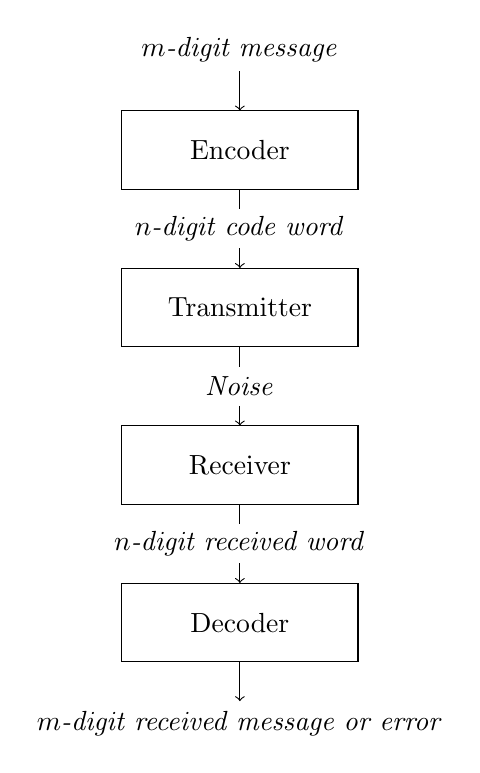
\begin{tikzpicture}[scale=1]

\draw [->] (0,8)  node [above] {\emph{$m$-digit message}} -- (0,7.5);

\node at (0,7) {Encoder};
\draw (-1.5,6.5) rectangle (1.5,7.5);
\draw (0,6.5)  -- (0,6.25);
\draw [->] (0,5.75)  -- (0,5.5);
\node at (0,6) {\emph{$n$-digit code word}};

\node at (0,5) {Transmitter};
\draw (-1.5,4.5) rectangle (1.5,5.5);
\draw (0,4.5)  -- (0,4.25);
\draw [->] (0,3.75)  -- (0,3.5);
\node at (0,4) {\emph{Noise}};

\node at (0,3) {Receiver};
\draw (-1.5,2.5) rectangle (1.5,3.5);
\draw (0,2.5)  -- (0,2.25);
\draw [->] (0,1.75)  -- (0,1.5);
\node at (0,2) {\emph{$n$-digit received word}};

\node at (0,1) {Decoder};
\draw (-1.5,0.5) rectangle (1.5,1.5);
\draw [->] (0,0.5)  -- (0,0) node [below] {\emph{$m$-digit received message or error}};

\end{tikzpicture}

\caption{Encoding and decoding messages}
\end{center}
\label{encoding}
\end{figure}

Uncoded messages may be composed of letters or characters, but
typically they consist of binary $m$-tuples. These messages are
encoded into codewords, consisting of binary $n$-tuples, by a device
called an \boldemph{encoder}. The message is transmitted and then decoded.
We will consider the occurrence of errors during transmission. An
\boldemph{error} occurs if there is a change in one or more bits in the
codeword. A \boldemph{decoding scheme} is a method that either converts
an arbitrarily received $n$-tuple into a meaningful decoded message or
gives an error message for that $n$-tuple. If the received message is
a codeword (one of the special $n$-tuples allowed to be transmitted),
then the decoded message must be the unique message that was encoded
into the codeword. For received non-codewords, the decoding scheme will
give an error indication, or, if we are more clever, will actually try
to correct the error and reconstruct the original message. Our goal is
to transmit error-free messages as cheaply and quickly as possible.
 
 
\begin{example}{repeat}
One possible coding scheme would be to send a message several
times and to compare the received copies with one another. Suppose
that the message to be encoded is a binary $n$-tuple $(x_{1}, x_{2},
\ldots, x_{n})$. The message is encoded into a binary $3n$-tuple by
simply repeating the message three times: 
\[
(x_{1}, x_{2}, \ldots, x_{n})
\mapsto
(x_{1}, x_{2}, \ldots, x_{n}, x_{1}, x_{2}, \ldots, x_{n},
x_{1}, x_{2}, \ldots, x_{n}).
\]
To decode the message, we choose as the $i$th digit the one that
appears in the $i$th place in at least two of the three transmissions.
For example, if the original message is $(0110)$, then the transmitted
message will be \mbox{$(0110\;  0110\;  0110)$}. If there is a transmission error
in the fifth digit, then the received codeword will be
$(0110\;  1110\;  0110)$, which will be correctly decoded as
$(0110)$.\footnote{We will adopt the convention that bits are numbered
left to right in binary $n$-tuples.} 
This triple-repetition method will automatically detect and correct
all single errors, but it is slow and inefficient: to send a message
consisting of $n$ bits, $2n$ extra bits are required, and we can only
detect and correct single errors. We will see that it is possible to
find an encoding scheme that will encode a message of $n$ bits into
$m$ bits with $m$ much smaller than $3n$.
\end{example}
 
 
\begin{example}{even_parity}
\boldemph{Even parity}, a  commonly  used coding scheme, is much
more efficient than the simple repetition scheme. The ASCII (American
Standard Code for Information Interchange) coding system uses binary
8-tuples, yielding $2^{8} = 256$ possible 8-tuples. However, only seven
bits are needed since there are only $2^7 = 128$ ASCII characters.
What can or should be done with the extra bit? Using the full eight
bits, we can detect single transmission errors. For example, the ASCII
codes for A, B, and C are 
\begin{align*}
\mbox{A} & = 65_{10} = 01000001_{2}, \\
\mbox{B} & = 66_{10} = 01000010_{2}, \\
\mbox{C} & = 67_{10} = 01000011_{2}.
\end{align*}
Notice that the leftmost bit is always set to 0; that is, the 128 ASCII
characters have codes 
\begin{align*}
00000000_{2} & = 0_{10}, \\
& \vdots \\
01111111_{2} & = 127_{10}.
\end{align*}
The bit can be used for error checking on the other seven bits. It is
set to either 0 or 1 so that the total number of 1 bits in the
representation of a character is even. Using even parity, the codes
for A, B, and C now become 
\begin{align*}
\mbox{A} & = 01000001_{2}, \\
\mbox{B} & = 01000010_{2}, \\
\mbox{C} & = 11000011_{2}.
\end{align*}
Suppose an A is sent and a transmission error in the sixth
bit is caused by noise over the communication channel so that 
(0100\; 0101) is received. We know an error has occurred since the
received word has an odd number of 1's, and we can now request that the
codeword be transmitted again. When used for error checking, the
leftmost bit is called a \boldemph{parity check bit}.  
 
 
By far the most common error-detecting
codes used in computers are based on the addition of a parity bit.
Typically, a computer stores information in $m$-tuples called \boldemph{
words}. Common word lengths are 8, 16, and 32 bits. One bit in the 
word is set aside as the parity check bit, and is not used to store
information. This bit is set to either 0 or 1, depending on the
number of 1's in the word. 
 
 
Adding a parity check bit allows the detection of all single errors
because changing a single bit either increases or decreases the number
of 1's by one, and in either case the parity has been changed from
even to odd, so the new word is not a codeword. (We could also
construct an error detection scheme based on \boldemph{odd parity}; that
is, we could set the parity check bit so that a codeword always has an
odd number of 1's.)  
\end{example}
 
 
The even parity system is easy to implement, but has two drawbacks.
First, multiple errors are not detectable. Suppose an A is sent and 
the first and seventh bits are changed from 0 to 1. The received word
is a codeword, but will be decoded into a C instead of an A.
Second, we do not have the ability to correct errors.  If the 8-tuple
(1001\; 1000) is received, we know that an error has occurred, but we
have no idea which bit has been changed. We will now investigate a
coding scheme that will not only allow us to detect transmission
errors but will actually correct the errors. 

 
 
\begin{table}[htb]\label{repetition_code}
\begin{center}{\small
\begin{tabular}{|lc|cccccccc|}
\hline
& & \multicolumn{8}{|c|}{Received Word}    \\
            &     & 000 & 001 & 010 & 011 & 100 & 101 & 110
& 111 \\ \hline
Transmitted & 000 & 0   & 1   & 1   & 2   & 1   & 2   & 2
& 3 \\
Codeword   & 111 & 3   &  2  & 2   &  1  &  2  &   1 &  1
&  0 \\ \hline
\end{tabular}
}
\caption{A repetition code}
\end{center}
\end{table}

 
\begin{example}{nearest}
Suppose that our original message is either a 0 or a 1, and that 0
encodes to (000) and 1 encodes to (111). If only a single
error occurs during transmission, we can detect and correct the
error. For example, if a 101 is received, then the second bit must
have been changed from a 1 to a 0.  The originally transmitted
codeword must have been (111). 	This method will detect and correct 
all single errors. 
 
 
In Table~\ref{repetition_code}, we present all possible words that might be received
for the transmitted codewords (000) and (111). Table~\ref{repetition_code} also shows 
the number of bits by which each received 3-tuple differs from each
original codeword. 
\end{example}
 
 
 
\subsection*{Maximum-Likelihood Decoding}

%% Footnote in subsection header undigestable by tex4ht
%%   it can follow just outside the {},
%%   but formats weirdly in both PDF and XHTML
%% \footnote{This section
%% requires a knowledge of probability, but can be
%% skipped without loss of continuity.}

%Label repaired.  Suggested by R. Beezer.
%TWJ - 12/19/2011
The coding scheme presented in Example~\ref{example:algcodes:nearest} is not a complete solution to
the problem because it does not account for the possibility of
multiple errors. For example, either a (000) or a (111) could be sent
and a (001) received. We have no means of deciding from the received
word whether there was a single error in the third bit or two errors,
one in the first bit and one in the second.  No matter what coding 
scheme is used, an incorrect message could
be received: we could transmit a (000), have errors in all three
bits, and receive the codeword (111). It is important to make explicit
assumptions about the likelihood and distribution of transmission
errors so that, in a particular application, it will be known whether
a given
error detection scheme is appropriate. We will assume that
transmission errors are rare, and, that when they do occur, they occur
independently in each bit; that is, if $p$ is the probability of an
error in one bit and $q$ is the probability of an error in a different
bit, then the probability of errors occurring in both of these bits at
the same time is $pq$. We will also assume that a received $n$-tuple 
is
decoded into a codeword that is closest to it; that is, we assume that
the receiver uses \boldemph{maximum-likelihood
decoding}\index{Maximum-likelihood decoding}.
 
 
\begin{figure}[htb]  %Replaced figure with tikz figure - TWJ 5/10/2010
\begin{center}
\tikzpreface{algcode_binary_channel}
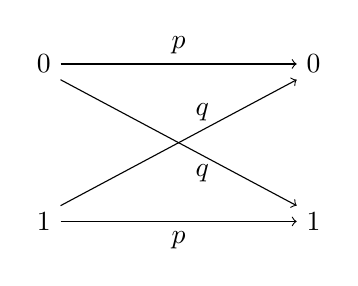
\begin{tikzpicture}[scale=1]

\node at (1.5,0) [below] {$p$};
\draw [->] (0,0)  node [left] {1} -- (3,0) node [right] {1};
\node at (1.5,2) [above] {$p$};
\draw [->] (0,2)  node [left] {0} -- (3,2) node [right] {0};

\draw [->] (0,0.2) -- (3,1.8);
\draw [->] (0,1.8) -- (3,0.2);

\node at (1.8,1.15) [above] {$q$};
\node at (1.8,0.85) [below] {$q$};


\end{tikzpicture}

\end{center}
\caption{Binary symmetric channel}
\label{channel}
\end{figure}
 
 
 
A \boldemph{binary symmetric channel}\index{Binary symmetric channel}
is a model that consists of a transmitter capable of sending a binary 
signal, either a 0 or a 1, together with a receiver. Let $p$ be the 
probability that the signal is correctly
received. Then $q=1-p$ is the probability of an incorrect reception.
If a 1 is sent, then the probability that a 1 is received is $p$ and
the probability that a 0 is received is $q$ (Figure~\ref{channel}).
The probability that no errors occur during the transmission of a binary
codeword of length $n$ is $p^{n}$. For example, if $p=0.999$ and a
message consisting of 10,000 bits is sent, then the probability of a
perfect transmission is 
\[
(0.999)^{10,000} \approx 0.00005.
\]
 
 
\begin{theorem}
If a binary $n$-tuple $(x_{1}, \ldots, x_{n})$ is transmitted across a
binary symmetric channel with probability $p$ that no error will occur
in each coordinate, then the probability that there are errors in
exactly $k$ coordinates~is
\[
\binom{n}{k} q^kp^{n-k}.
\]
\end{theorem}
 
 
\begin{proof}
Fix $k$ different coordinates. We first compute the probability that
an error has occurred in this fixed set of coordinates. The
probability of an error occurring in a particular one of these $k$
coordinates is $q$; the probability that an error will not occur
in any of the remaining $n-k$ coordinates is $p$. The
probability of each of these $n$ independent events is
$q^{k}p^{n-k}$. The number of possible error patterns with exactly $k$
errors occurring is equal to 
\[
\binom{n}{k} 
= \frac{n!}{k!(n-k)!},
\]
the number of combinations of $n$ things taken $k$ at a time. Each of
these error patterns has probability $q^{k}p^{n-k}$ of occurring;
hence, the probability of all of these error patterns is
\[
\binom{n}{k} 
q^{k}p^{n-k}.
\]
\end{proof}
 
 
\begin{example}{probability}
Suppose that $p = 0.995$ and a 500-bit message is sent. The
probability that the message was sent error-free is 
\[
p^{n} = (0.995)^{500} \approx 0.082.
\]
The probability of exactly one error occurring is
\[
\binom{n}{1} 
qp^{n-1}= 500(0.005)(0.995)^{499}
\approx 0.204.
\]
The probability of exactly two errors is
\[
\binom{n}{2} 
q^{2}p^{n-2}=
\frac{500 \cdot 499}{2}(0.005)^{2}(0.995)^{498} \approx
0.257.
\]
The probability of more than two errors is approximately
\[
1-0.082-0.204 -0.257=0.457.
\]
\end{example}
 
 
\subsection*{Block Codes}
 
 
If we are to develop efficient error-detecting and error-correcting
codes, we will need more sophisticated mathematical tools.  Group
theory  will allow faster methods of encoding and decoding messages. A
code is an $(n, m)$-\boldemph{block code} if the information that is to be
coded can be divided into blocks of $m$ binary digits, each of which
can be encoded into $n$ binary digits. More specifically, an $(n,
m)$-block code consists of an \boldemph{encoding function} 
\[
E:{\mathbb Z}^{m}_{2} \rightarrow {\mathbb Z}^{n}_{2}
\]
and a \boldemph{decoding function}
\[
D:{\mathbb Z}^{n}_{2} \rightarrow {\mathbb Z}^{m}_{2}.
\]
A \boldemph{codeword} is any element in the image of $E$. We also require
that $E$ be one-to-one so that two information blocks will not be
encoded into the same codeword. If our code is to be error-correcting,
then $D$ must be onto.
 
 
\begin{example}{BlockCode}
The even-parity coding system developed to detect single errors in
ASCII characters is an $(8,7)$-block code. The encoding function is
\[
E(x_7, x_6, \ldots, x_1) = (x_8, x_7,  \ldots, x_1),
\]
where $x_8 = x_7 + x_6 + \cdots + x_1$ with addition in ${\mathbb Z}_2$. 
\end{example}
 

 
Let ${\mathbf x} = (x_1, \ldots, x_n)$ and ${\mathbf y} = (y_1, \ldots,
y_n)$ be binary $n$-tuples. The \boldemph{Hamming distance}\index{Hamming
distance} or \boldemph{distance}, $d({\mathbf x}, {\mathbf
y})$\label{noteHammingdist}, between ${\mathbf x}$ and ${\mathbf y}$ is
the number of bits in which ${\mathbf x}$ and ${\mathbf y}$ differ. The
distance between two codewords is the minimum number of transmission
errors required to change one codeword into the other. The
\boldemph{minimum distance}\index{Code!minimum distance of} for a code,
$d_{\min}$\label{notemindist}, is the minimum of all distances
$d({\mathbf x}, {\mathbf y})$, where ${\mathbf x}$ and ${\mathbf y}$ are
distinct codewords. The \boldemph{weight}\index{Weight of a codeword},
$w({\mathbf x})$\label{noteweight}, of a binary codeword ${\mathbf x}$ is
the number of 1's in ${\mathbf x}$. Clearly, $w({\mathbf x}) = d({\mathbf
x}, {\mathbf 0})$, where ${\mathbf 0} = (00 \cdots 0)$. 
 
 
\begin{example}{min_distance}
Let ${\mathbf x} = (10101)$, ${\mathbf y} = (11010)$, and ${\mathbf z} =
(00011)$ be all of the codewords in some code $C$. Then we have the
following Hamming distances: 
\[
d({\mathbf x},{\mathbf y}) = 4, \qquad
d({\mathbf x},{\mathbf z}) = 3, \qquad
d({\mathbf y},{\mathbf z}) = 3.
\]
The minimum distance  for this code is 3. We also have the
following weights: 
\[
w({\mathbf x}) = 3, \qquad
w({\mathbf y}) = 3, \qquad
w({\mathbf z}) = 2.
\]
\end{example}
 
 
The following proposition lists some basic properties about the weight
of a codeword and the distance between two codewords. The proof is
left as an exercise.
 
 
\begin{proposition}
Let ${\mathbf x}$, ${\mathbf y}$, and ${\mathbf z}$ be binary $n$-tuples.
Then 
\begin{enumerate}
 
\rm \item \it
$w({\mathbf x}) = d( {\mathbf x}, {\mathbf 0})$; 
 
\rm \item \it
$d( {\mathbf x}, {\mathbf y}) \geq 0$; 
 
\rm \item \it
$d( {\mathbf x}, {\mathbf y}) = 0$ exactly when ${\mathbf x} = {\mathbf y}$; 
 
\rm \item \it
$d( {\mathbf x}, {\mathbf y})= d( {\mathbf y}, {\mathbf x})$; 
 
\rm \item \it
$d( {\mathbf x}, {\mathbf y}) \leq d( {\mathbf x}, {\mathbf z}) + d( {\mathbf
z}, {\mathbf y})$. 
 
\end{enumerate}
\end{proposition}
 
 
The weights in a particular code are usually much easier to compute
than the Hamming distances between all codewords in the code. If a
code is set up carefully, we can use this fact to our advantage.
 
 
Suppose that ${\mathbf x} = (1101)$ and ${\mathbf y} = (1100)$ are
codewords in some code. If we transmit (1101) and an error occurs in
the rightmost bit, then (1100) will be received. Since (1100) is a
codeword, the decoder will decode (1100) as the transmitted message.
This code is clearly not very appropriate for error detection. The
problem is that $d({\mathbf x}, {\mathbf y}) = 1$. If ${\mathbf x} = (1100)$
and ${\mathbf y} = (1010)$ are codewords, then $d({\mathbf x}, {\mathbf y})
= 2$. If ${\mathbf x}$ is transmitted and a single error occurs, then
${\mathbf y}$ can never be received. Table~\ref{4-bit_words} gives the distances
between all 4-bit codewords in which the first three bits carry
information and the fourth is an even parity check bit. We can see
that the minimum distance here is 2; hence, the code is suitable as
a single error-correcting code. 
 
 
\begin{table}[hbt]
{\small
\begin{center}
\begin{tabular}{|c|cccccccc|}
\hline
    & 0000 & 0011 & 0101 & 0110 & 1001 & 1010 & 1100 & 1111
\\ \hline
0000 & 0 & 2 & 2 & 2 & 2 & 2 & 2 & 4 \\
0011 & 2 & 0 & 2 & 2 & 2 & 2 & 4 & 2 \\
0101 & 2 & 2 & 0 & 2 & 2 & 4 & 2 & 2 \\
0110 & 2 & 2 & 2 & 0 & 4 & 2 & 2 & 2 \\
1001 & 2 & 2 & 2 & 4 & 0 & 2 & 2 & 2 \\
1010 & 2 & 2 & 4 & 2 & 2 & 0 & 2 & 2 \\
1100 & 2 & 4 & 2 & 2 & 2 & 2 & 0 & 2 \\
1111 & 4 & 2 & 2 & 2 & 2 & 2 & 2 & 0 \\
\hline
\end{tabular}
\caption{Distances between 4-bit codewords}\label{4-bit_words}
\end{center}
}
\end{table}
 
 
 
To determine exactly what the error-detecting and error-correcting
capabilities for a code are, we need to analyze the minimum distance
for the code. Let ${\mathbf x}$ and ${\mathbf y}$ be codewords. If
$d({\mathbf x}, {\mathbf y}) = 1$ and an error occurs where ${\mathbf x}$
and ${\mathbf y}$ differ, then ${\mathbf x}$ is changed to ${\mathbf y}$.
The received codeword is ${\mathbf y}$ and no error message is given.
Now suppose $d({\mathbf x}, {\mathbf y}) = 2$. Then a single error cannot
change ${\mathbf x}$ to ${\mathbf y}$. Therefore, if $d_{\min} = 2$, we
have the ability to detect single errors. However, suppose that
$d({\mathbf x}, {\mathbf y}) = 2$, ${\mathbf y}$ is sent, and a noncodeword
${\mathbf z}$ is received such that
\[
d({\mathbf x}, {\mathbf z}) = d({\mathbf y}, {\mathbf z}) = 1.
\]
Then the decoder cannot decide between ${\mathbf x}$ and ${\mathbf y}$. Even
though we are aware that an error has occurred, we do not know what
the error is.
 
 
Suppose $d_{\min} \geq 3$. Then the maximum-likelihood decoding scheme
corrects all single errors. Starting with a codeword ${\mathbf x}$, an
error in the transmission of a single bit gives ${\mathbf y}$ with
$d({\mathbf x}, {\mathbf y}) = 1$, but $d({\mathbf z}, {\mathbf y}) \geq 2$
for any other codeword ${\mathbf z} \neq {\mathbf x}$. If we do not
require the correction of errors, then we can detect multiple errors
when a code has a minimum distance that is greater than 3.  
 
 
\begin{theorem}\label{algecodes:min_distance_theorem}
Let $C$ be a code with $d_{\min} = 2n + 1$. Then $C$ can correct any
$n$ or fewer errors.  Furthermore, any $2n$ or fewer errors can be
detected in~$C$. 
\end{theorem}
 
 
\begin{proof}
Suppose that a codeword ${\mathbf x}$ is sent and the word ${\mathbf y}$
is received with at most $n$ errors. Then $d( {\mathbf x}, {\mathbf y})
\leq n$. If ${\mathbf z}$ is any codeword other than ${\mathbf x}$, then
\[
2n+1
\leq
d( {\mathbf x}, {\mathbf z})
\leq
d( {\mathbf x}, {\mathbf y}) + d( {\mathbf y}, {\mathbf z})
\leq
n + d( {\mathbf y}, {\mathbf z}).
\]
Hence, $d({\mathbf y}, {\mathbf z} ) \geq n+1$ and ${\mathbf y}$ will be
correctly decoded as ${\mathbf x}$. Now suppose that ${\mathbf x}$ is
transmitted and ${\mathbf y}$ is received and that at least one error 
has occurred, but not more than $2n$ errors. Then $1 \leq d( {\mathbf x},
{\mathbf y} ) \leq 2n$.  Since the minimum distance between codewords is
$2n +1$, ${\mathbf y}$ cannot be a codeword.  Consequently, the code can
detect between 1 and $2n$ errors. 
\end{proof}
 
 
\begin{example}{single_correct}
In Table~\ref{Hamming_dist}, the codewords ${\mathbf c}_1 = (00000)$, ${\mathbf c}_2 = (00111)$,
${\mathbf c}_3 = (11100)$, and ${\mathbf c}_4 = (11011)$ determine a
single error-correcting code.  
\end{example}
 
 
\begin{table}[htb]

\begin{center}
{\small
\begin{tabular}{|c|cccc|}
\hline
      & 00000 & 00111 & 11100 & 11011 \\ \hline
00000 & 0     & 3     & 3     & 4 \\
00111 & 3     & 0     & 4     & 3 \\
11100 & 3     & 4     & 0     & 3 \\
11011 & 4     & 3     & 3     & 0 \\
\hline
\end{tabular}
}
\caption{ Hamming distances for an error-correcting code}\label{Hamming_dist}
\end{center}
\end{table}
 
 
 
 
 
\histhead
 
 
\noindent{\small \histf
Modern coding theory began in 1948 with C. Shannon's\index{Shannon,
C.} paper, ``A Mathematical Theory of Information'' [7]. This paper offered
an example of an algebraic code, and Shannon's Theorem proclaimed
exactly how good codes could be expected to be. Richard
Hamming\index{Hamming, R.} began working with linear codes at Bell
Labs in the late 1940s and early 1950s after becoming frustrated
because the programs that he was running could not recover from simple
errors generated by noise. Coding theory has grown tremendously in the
past several years. \textit{The Theory of Error-Correcting Codes}, by 
MacWilliams and Sloane [5], published in 1977, already
contained over 1500 references. Linear codes (Reed-Muller $(32,
6)$-block codes) were used on NASA's Mariner space probes.  More recent
space probes such as Voyager have used what are called convolution
codes.  Currently, very active research is being done with Goppa
codes, which are heavily dependent on algebraic geometry.
\histbox
} 
 
 
\section{Linear Codes}
 
 
To gain more knowledge of a particular code and develop more efficient
techniques of encoding, decoding, and error detection, we need to add
additional structure to our codes. One way to accomplish this is to
require that the code also be a group. A \boldemph{group
code}\index{Code!group} is a code that is also a subgroup of ${\mathbb
Z}_2^n$.  
 
 
To check that a code is a group code, we need only verify one thing.
If we add any two elements in the code, the result must be an $n$-tuple
that is again in the code. It is not necessary to check that the
inverse of the $n$-tuple is in the code, since every codeword is its own
inverse, nor is it necessary to check that ${\mathbf 0}$ is a codeword.
For instance,
\[
(11000101) + (11000101) = (00000000).
\]
 
 
\begin{example}{weights}
Suppose that we have a code that consists of the following 7-tuples: 
\[
\begin{array}{cccc}
(0000000) & (0001111) & (0010101) & (0011010) \\
(0100110) & (0101001) & (0110011) & (0111100) \\
(1000011) & (1001100) & (1010110) & (1011001) \\
(1100101) & (1101010) & (1110000) & (1111111).
\end{array}
\]
It is a straightforward though tedious task to verify that this code
is also a subgroup of ${\mathbb Z}_2^7$ and, therefore, a group code.
This code is a single error-detecting and single error-correcting 
code, but
it is a long and tedious process to compute all of the distances
between  pairs of codewords to determine that $d_{\min} = 3$. It is
much easier to see that the minimum weight of all the nonzero
codewords is 3. As we will soon see, this is no coincidence.
However, the relationship between weights and distances in a
particular code is heavily dependent on the fact that the code is a
group. 
\end{example}
 
 
\begin{lemma}
Let ${\mathbf x}$ and ${\mathbf y}$ be  binary $n$-tuples. Then $w({\mathbf
x} + {\mathbf y}) = d({\mathbf x}, {\mathbf y})$. 
\end{lemma}
 
 
\begin{proof}
Suppose that ${\mathbf x}$ and ${\mathbf y}$ are binary $n$-tuples. Then
the distance between ${\mathbf x}$ and ${\mathbf y}$ is exactly the number
of places in which ${\mathbf x}$ and ${\mathbf y}$ differ. But ${\mathbf x}$
and ${\mathbf y}$ differ in a particular coordinate exactly when the sum
in the coordinate is 1, since
\begin{align*}
1 + 1 & = 0 \\
0 + 0 & = 0 \\
1 + 0 & = 1 \\
0 + 1 & = 1.
\end{align*}
Consequently, the weight of the sum must be the distance between the two
codewords.
\end{proof}
 
 
\begin{theorem}
Let $d_{\min}$ be the minimum distance for a group code $C$. Then
$d_{\min}$ is the minimum of all the nonzero weights of the nonzero
codewords in $C$. That is, 
\[
d_{\min} = \min\{ w({\mathbf x}) : { {\mathbf x} \neq {\mathbf 0} } \}.
\]
\end{theorem}
 
 
\begin{proof}
Observe that
\begin{align*}
d_{\min} & =  \min \{ d({\mathbf x},{\mathbf y}) : {\mathbf x}
\neq
{\mathbf y} \} \\
&=  \min \{ d({\mathbf x},{\mathbf y}) : {\mathbf x}+{\mathbf y}
\neq {\mathbf 0} \} \\
&= \min\{ w({\mathbf x} + {\mathbf y}) : {\mathbf x}+{\mathbf y}
\neq {\mathbf 0} \} \\
& =  \min\{ w({\mathbf z}) : {\mathbf z} \neq {\mathbf 0} \}.
\end{align*}
\end{proof}
 
 
\subsection*{Linear Codes}
 
 
From Example~\ref{example:algcodes:weights}, it is now easy to check that the minimum nonzero
weight is 3; hence, the code does indeed detect and correct all
single errors. We have now reduced the problem of finding ``good''
codes to that of generating group codes. One easy way to generate
group codes is to employ a bit of matrix theory. 
 
 
Define the \boldemph{inner product}\index{Inner product} of two binary
$n$-tuples to be 
\[
{\mathbf x} \cdot {\mathbf y} = x_1 y_1 + \cdots + x_n y_n,
\]
where ${\mathbf x} = (x_1, x_2, \ldots, x_n)^{\rm t}$ and ${\mathbf y} =
(y_1, y_2, \ldots, y_n)^{\rm t}$ are column vectors.\footnote{Since we
will be working with matrices, we will write binary $n$-tuples as
column vectors for the remainder of this chapter.} For example, if
${\mathbf x} = (011001)^{\rm t}$ and ${\mathbf y} = (110101)^{\rm t}$,
then ${\mathbf x} \cdot {\mathbf y} = 0$. We can also look at an inner
product as the product of a row matrix with a column matrix; that is, 
\begin{align*}
{\mathbf x} \cdot {\mathbf y} & = {\mathbf x}^{\rm t}  {\mathbf y}
\\
& =
\begin{pmatrix}
x_1 & x_2 & \cdots & x_n
\end{pmatrix}
\begin{pmatrix}
y_1 \\
y_2 \\
\vdots \\
y_n
\end{pmatrix} \\
& =
x_{1}y_{1} + x_{2}y_{2} + \cdots + x_{n}y_{n}.
\end{align*}
 
 
\begin{example}{matrix_codes}
Suppose that the words to be encoded consist of all binary
\mbox{3-tuples}
and that our encoding scheme is even-parity. To encode an arbitrary
3-tuple, we add a fourth bit to obtain an even number of 1's. Notice
that an arbitrary $n$-tuple ${\mathbf x} = (x_1, x_2, \ldots, x_n)^{\rm
t}$ has an even number of 1's exactly when $x_1 + x_2 + \cdots + x_n =
0$; hence, a 4-tuple ${\mathbf x} = (x_1, x_2, x_3, x_4)^{\rm t}$ has an
even number of 1's if $ x_1+ x_2+ x_3+ x_4 = 0$, or 
\[
{\mathbf x} \cdot {\mathbf 1} 
= 
{\mathbf x}^{\rm t} {\mathbf 1} 
=
\begin{pmatrix}
x_1 & x_2 & x_3 & x_4
\end{pmatrix}
\begin{pmatrix}
1 \\ 1 \\ 1 \\ 1
\end{pmatrix} = 0.
\]
This example leads us to hope that there is a connection between
matrices and coding theory. 
\end{example}
 
 
Let ${\mathbb M}_{m \times n}({\mathbb Z}_2)$\label{notembyn} denote the set
of all $m \times n$ matrices with entries in ${\mathbb Z}_2$. We do
matrix operations as usual except that all our addition and multiplication
operations occur in ${\mathbb Z}_2$. Define the \boldemph{null
space}\index{Matrix!null space of}\index{Null space!of a matrix} of 
a matrix $H \in {\mathbb M}_{m \times n}({\mathbb Z}_2)$ to be the set of
all binary $n$-tuples ${\mathbf x}$ such that $H{\mathbf x} = {\mathbf 0}$.
We denote the null space of a matrix $H$ by ${\rm Null}(H)$\label{notenull}.  
 
 
\begin{example}{group_code}
Suppose that
\[
H =
\begin{pmatrix}
0 & 1 & 0 & 1 & 0 \\
1 & 1 & 1 & 1 & 0 \\
0 & 0 & 1 & 1 & 1
\end{pmatrix}.
\]
For a 5-tuple ${\mathbf x} = (x_1, x_2, x_3, x_4, x_5)^{\rm t}$ to be in
the null space of $H$, $H{\mathbf x} = {\mathbf 0}$. Equivalently, the
following system of equations must be satisfied:   
\begin{align*}
  x_2 +  x_4  & =  0 \\
x_1 +  x_2 + x_3  + x_4   & =  0 \\
  x_3  + x_4  +  x_5 & =  0.
\end{align*}
The set of binary 5-tuples satisfying these equations is
\[
(00000) \qquad (11110) \qquad (10101) \qquad (01011).
\]
This code is easily determined to be a group code.
\end{example}
 
 
\begin{theorem}
Let $H$ be in ${\mathbb M}_{m \times n}({\mathbb Z}_2)$. Then the null space of
$H$ is a group~code. 
\end{theorem}
 
 
\begin{proof}
Since each element of ${\mathbb Z}_2^n$ is its own inverse, the only
thing that really needs to be checked here is closure. Let ${\mathbf x},
{\mathbf y} \in {\rm Null}(H)$ for some matrix $H$ in ${\mathbb M}_{m \times
n}({\mathbb Z}_2)$. Then $H{\mathbf x} = {\mathbf 0}$ and $H{\mathbf y} =
{\mathbf 0}$. So 
\[
H({\mathbf x}+{\mathbf y}) 
=
H{\mathbf x} + H{\mathbf y} = {\mathbf 0}
+
{\mathbf 0}
= {\mathbf 0}.
\]
Hence, ${\mathbf x}+{\mathbf y}$ is in the null space of $H$ and
therefore must be a codeword. 
\hspace*{1in}
\end{proof}
 
%typo correction.  Suggested by J. Buller.
%TWJ - 12/20/2011

\medskip
 
 
A code is a \boldemph{linear code}\index{Code!linear} if it is
determined by the null space of some matrix $H \in {\mathbb M}_{m \times
n}({\mathbb Z}_2)$.  
 
 
 
\begin{example}{linear_code}
Let $C$ be the code given by the matrix
\[
H =
\begin{pmatrix}
0 & 0 & 0 & 1 & 1 & 1 \\
0 & 1 & 1 & 0 & 1 & 1 \\
1 & 0 & 1 & 0 & 0 & 1
\end{pmatrix}.
\]
Suppose that the 6-tuple ${\mathbf x} = (010011)^{\rm t}$ is received.
It is a simple matter of matrix multiplication to determine whether or
not ${\mathbf x}$ is a codeword. Since 
\[
H{\mathbf x} =
\begin{pmatrix} 
0 \\ 1 \\ 1
\end{pmatrix},
\]
the received word is not a codeword.  We must either attempt to
correct the word or request that it be transmitted again.
\end{example}

%typo correction.  Suggested by J. Buller.
%TWJ - 12/20/2011
 
 
 
\section{Parity-Check and Generator Matrices}
 
 
We need to find a systematic way of generating linear codes as well as
fast methods of decoding. By examining the properties of a matrix $H$
and by carefully choosing $H$, it is possible to develop very
efficient methods of encoding and decoding messages. To this end, we 
will introduce standard generator and canonical parity-check
matrices.
 
 
Suppose that $H$ is an $m \times n$ matrix with entries in
${\mathbb Z}_2$ and $n > m$. If the last $m$ columns of the
matrix form the $m \times m$ identity matrix, $I_m$, then
the matrix is a \boldemph{canonical parity-check
matrix}\index{Matrix!parity-check}. More specifically, $H= (A \mid I_m
)$, where $A$ is the $m \times (n-m)$ matrix
\[
\begin{pmatrix}
a_{11} & a_{12} & \cdots & a_{1,n-m} \\
a_{21} & a_{22} & \cdots & a_{2,n-m} \\
\vdots & \vdots \ddots & \vdots    \\
a_{m1} & a_{m2} & \cdots & a_{m,n-m}
\end{pmatrix}
\]
and $I_m$ is the $m \times m$ identity matrix
\[
\begin{pmatrix}
1 & 0 & \cdots & 0 \\
0 & 1 & \cdots & 0 \\
\vdots & \vdots \ddots & \vdots \\
0 & 0 & \cdots & 1
\end{pmatrix}.
\]
With each canonical parity-check matrix we can associate an $n \times
(n-m)$ \boldemph{standard generator matrix}\index{Matrix!generator} 
\[
G =
\left(
\frac{I_{n-m}}{A}
\right).
\]
Our goal will be to show that $G {\mathbf x} = {\mathbf y}$ if and only if
$H{\mathbf y} = {\mathbf 0}$.  Given a message block ${\mathbf x}$ to be
encoded, $G$ will allow us to quickly encode it into a linear
codeword ${\mathbf y}$. 
 
 
\begin{example}{ParityCheck}
Suppose that we have the following eight words to be
encoded:
\[
(000), (001), (010), \ldots, (111).
\]
For
\[
A =
\begin{pmatrix}
0 & 1 & 1 \\
1 & 1 & 0 \\
1 & 0 & 1
\end{pmatrix},
\]
the associated standard generator and canonical parity-check matrices
are 
\[
G=
\begin{pmatrix}
1 & 0 & 0 \\
0 & 1 & 0 \\
0 & 0 & 1 \\
0 & 1 & 1 \\
1 & 1 & 0 \\
1 & 0 & 1
\end{pmatrix}
\]
and
\[
H =
\begin{pmatrix}
0 & 1 & 1 & 1 & 0 & 0 \\
1 & 1 & 0 & 0 & 1 & 0 \\
1 & 0 & 1 & 0 & 0 & 1
\end{pmatrix},
\]
respectively.
 
 
Observe that the rows in $H$  represent the parity checks on certain
bit positions in a 6-tuple. The 1's in the identity matrix serve as
parity checks for the 1's in the same row. If ${\mathbf x} = (x_1, x_2,
x_3, x_4, x_5, x_6)$, then 
\[
{\mathbf 0}
=
H{\mathbf x}
=
\begin{pmatrix}
x_2 + x_3 + x_4 \\
x_1 + x_2 + x_5\\
x_1 + x_3 + x_6
\end{pmatrix},
\]
which yields a system of equations:
\begin{align*}
x_2 + x_3 + x_4 & = 0 \\
x_1 + x_2 + x_5 & = 0 \\
x_1 + x_3 + x_6 & = 0.
\end{align*}
Here $x_4$ serves as a check bit for $x_2$ and $x_3$; $x_5$ is a check
bit for $x_1$ and $x_2$; and $x_6$ is a check bit for $x_1$ and $x_3$.
The identity matrix keeps $x_4$, $x_5$, and $x_6$ from having to check
on each other. Hence, $x_1$, $x_2$, and $x_3$ can be arbitrary but
$x_4$, $x_5$, and $x_6$ must be chosen to ensure parity. The null
space of $H$ is easily computed to be
\[
\begin{array}{cccc}
 (000000) & (001101) & (010110) & (011011) \\
 (100011) & (101110) & (110101) & (111000).
\end{array}
\]
An even easier way to compute the null space is with the generator
matrix $G$ (Table~\ref{matrix_gen_code}). 
\end{example}
 
 
\begin{table}[htb]
{\small
\begin{center}
\begin{tabular}{|c|c|}
\hline
Message Word  & Codeword \\
${\mathbf x}$ & $G {\mathbf x}$ \\ \hline
000 & 000000 \\
001 & 001101 \\
010 & 010110 \\
011 & 011011 \\
100 & 100011 \\
101 & 101110 \\
110 & 110101 \\
111 & 111000 \\
\hline
\end{tabular}
\end{center}
}
\caption{A matrix-generated code}\label{matrix_gen_code}
\end{table}
 
 
\begin{theorem}
If $H \in {\mathbb M}_{m \times n}({\mathbb Z}_2)$ is a canonical
parity-check matrix, then ${\rm Null}(H)$ consists of all 
${\mathbf x} \in {\mathbb Z}_2^n$ whose first $n-m$ bits are arbitrary but whose last $m$ bits
are determined by $H{\mathbf x} = {\mathbf 0}$. Each of
the last $m$ bits serves as an even parity check bit for some of the
first $n-m$ bits. Hence, $H$ gives rise to an $(n, n-m)$-block code. 
\end{theorem}


 
 
We leave the proof of this theorem as an exercise. In light of the
theorem, the first $n - m$ bits in ${\mathbf x}$ are called \boldemph{
information bits} and the last $m$ bits are called \boldemph{check bits}.
In Example~\ref{example:algcodes:ParityCheck},  the first three bits are the information bits
and the last three are the check bits.
 
 
\begin{theorem}
Suppose that $G$ is an $n \times k$  standard generator matrix.  Then
$C = \left\{{\mathbf y} : G{\mathbf x} ={\mathbf y}\text{ for }{\mathbf x}\in
{\mathbb  Z}_2^k\right\}$ is an  $(n,k)$-block code. More specifically, $C$
is a group code.  
\end{theorem}
 
 
\begin{proof}
Let $G {\mathbf x}_1 = {\mathbf y}_1$ and $G {\mathbf
x}_2 ={\mathbf y}_2$ be two codewords. Then ${\mathbf y}_1
+ {\mathbf y}_2$ is in $C$ since 
\[
G( {\mathbf x}_1 + {\mathbf x}_2)
=
G {\mathbf x}_1 + G {\mathbf x}_2
=
{\mathbf y}_1 + {\mathbf y}_2.
\]
We must also show that two message blocks cannot be encoded into the
same codeword. That is, we must show that if $G {\mathbf x} = G
{\mathbf y}$, then ${\mathbf x} = {\mathbf y}$.  Suppose that $G
{\mathbf x} = G {\mathbf y}$. Then
\[
G {\mathbf x} - G {\mathbf y}
=
G( {\mathbf x} - {\mathbf y})
=
{\mathbf 0}.
\]
However, the first $k$ coordinates in $G( {\mathbf x} - {\mathbf
y})$ are exactly $x_1 -y_1, \ldots, x_k - y_k$, since they are
determined by the identity matrix, $I_k$, part of $G$. Hence, $G(
{\mathbf x} - {\mathbf y}) = {\mathbf 0}$ exactly when
${\mathbf x} = {\mathbf y}$.
\end{proof}
 
 \medskip
 
 
Before we can prove the relationship between canonical parity-check
matrices and standard generating matrices, we need to prove a lemma.
 
 
\begin{lemma}\label{ParityCheckLemma}
Let $H = (A \mid I_m )$ be an $m \times n$ canonical parity-check
matrix and $G = \left( \frac{I_{n-m} }{A} \right)$ be the
corresponding $n \times (n-m)$ standard generator matrix. Then $HG =
{\mathbf 0}$. 
\end{lemma}
 
 
\begin{proof}
Let $C = HG$.  The $ij$th entry in $C$ is
\begin{align*}
c_{ij}
& = 
\sum_{k=1}^n h_{ik} g_{kj} \\
& =  \sum_{k=1}^{n-m} h_{ik} g_{kj} + \sum_{k=n-m+1}^n h_{ik} g_{kj} \\
& = \sum_{k=1}^{n-m} a_{ik} \delta_{kj} + \sum_{k=n-m+1}^n \delta_{i-(m-n),k} a_{kj} \\
& =  a_{ij} + a_{ij} \\
& = 0,
\end{align*}
where
\[
\delta_{ij}\label{notekron}
=
\begin{cases}
1, & i = j \\
0, & i \neq j
\end{cases}
\]
is the Kronecker delta\index{Kronecker delta}.
\end{proof}
 
 
\begin{theorem}
Let $H = (A \mid I_m )$ be an $m \times n$ canonical parity-check
matrix and let $G = \left( \frac{I_{n-m} }{A} \right) $ be the $n
\times (n-m)$ standard generator matrix associated with $H$. Let $C$
be the code generated by $G$. Then ${\mathbf y}$ is in $C$ if and only
if $H {\mathbf y} = {\mathbf 0}$. In particular, $C$ is a linear code with
canonical parity-check matrix $H$. 
\end{theorem}
 
 
\begin{proof}
First suppose that ${\mathbf y} \in C$. Then $G {\mathbf x} = {\mathbf y}$
for some ${\mathbf x} \in {\mathbb Z}_2^m$. By Lemma~\ref{ParityCheckLemma}, $H {\mathbf y} = HG
{\mathbf x} = {\mathbf 0}$. 
 
 
Conversely, suppose that ${\mathbf y} = (y_1, \ldots, y_n)^{\rm t}$ is
in the null space of $H$.  We need to find an ${\mathbf x}$ in ${\mathbb
Z}_2^{n-m}$ such that $G {\mathbf x}^{\rm t} = {\mathbf y}$. Since $H
{\mathbf y} = {\mathbf 0}$, the following set of equations must be
satisfied:  
\begin{align*}
a_{11} y_1 + a_{12} y_2 + \cdots + a_{1, n-m} y_{n-m} + y_{n-m+1}
& = 0 \\
a_{21} y_1 + a_{22} y_2 + \cdots + a_{2, n-m} y_{n-m} + y_{n-m+1}
& = 0 \\
& \vdots   \\
a_{m1} y_1 + a_{m2} y_2 + \cdots + a_{m, n-m} y_{n-m} + y_{n-m+1}
& = 0.
\end{align*}
Equivalently, $y_{n-m+1}, \ldots, y_n$ are determined by $y_1, \ldots,
y_{n-m}$: 
\begin{align*}
y_{n-m+1}
& = a_{11} y_1 + a_{12} y_2 + \cdots + a_{1, n-m} y_{n-m} \\
y_{n-m+1}
& = a_{21} y_1 + a_{22} y_2 + \cdots + a_{2, n-m} y_{n-m} \\
& \vdots \\
y_{n-m+1}
& = a_{m1} y_1 + a_{m2} y_2 + \cdots + a_{m, n-m} y_{n-m}.
\end{align*}
Consequently, we can let $x_i = y_i$ for $i= 1, \ldots, n - m$.
\end{proof}
 
 
\medskip
 
 
It would be helpful if we could compute the minimum distance of a
linear code directly from its matrix $H$ in order to determine the
error-detecting and error-correcting capabilities of the code. Suppose
that  
\begin{align*}
{\mathbf e}_1 & = (100 \cdots 00)^{\rm t} \\
{\mathbf e}_2 & = (010 \cdots 00)^{\rm t} \\
 & \vdots \\
{\mathbf e}_n & = (000 \cdots 01)^{\rm t}
\end{align*}
are the $n$-tuples in ${\mathbb Z}_2^n$ of weight 1. For an $m \times
n$ binary matrix $H$, $H{\mathbf e}_i$ is exactly the $i$th column of
the matrix $H$. 
 
 
\begin{example}{ith_column}
Observe that
\[
\begin{pmatrix}
1 & 1 & 1 & 0 & 0 \\
1 & 0 & 0 & 1 & 0 \\
1 & 1 & 0 & 0 & 1
\end{pmatrix}
\begin{pmatrix}
 0 \\ 1 \\ 0 \\ 0 \\ 0
\end{pmatrix}
=
\begin{pmatrix}
1 \\ 0 \\ 1
\end{pmatrix}.
\]
\end{example}
 
 
We state this result in the following proposition and leave the proof
as an exercise. 
 
\begin{proposition}\label{ColumnProp}
Let ${\mathbf e}_i$ be the binary $n$-tuple with a $1$ in the $i$th
coordinate and $0$'s elsewhere and suppose that $H \in {\mathbb M}_{m
\times n}({\mathbb Z}_2)$. Then $H{\mathbf e}_i$ is the $i$th column of
the matrix $H$.  
\end{proposition}
 
 
\begin{theorem}\label{SingleErrorTheorem}
Let $H$ be an $m \times n$ binary matrix. Then the null space of $H$
is a single error-detecting code if and only if no column of $H$
consists entirely of zeros. 
\end{theorem}
 
 
\begin{proof}
Suppose that ${\rm Null}(H)$ is a single error-detecting code. Then the minimum
distance of the code must be at least 2. Since the null space is a
group code, it is sufficient to require that the code contain no
codewords of less than weight 2 other than the zero codeword. That
is, ${\mathbf e}_i$ must not be a codeword for $i = 1, \ldots, n$. Since
$H{\mathbf e}_i$ is the $i$th column of $H$, the only way in which
${\mathbf e}_i$ could be in the null space of $H$ would be if the $i$th
column were all zeros, which is impossible; hence, the code must have
the capability to detect at least single errors.
 
 
Conversely, suppose that no column of $H$ is the zero column. By 
Proposition~\ref{ColumnProp}, $H{\mathbf e}_i \neq {\mathbf 0}$.
\end{proof}
 
 
\begin{example}{null_space}
If we consider the matrices
\[
H_1 =
\begin{pmatrix}
1 & 1 & 1 & 0 & 0 \\
1 & 0 & 0 & 1 & 0 \\
1 & 1 & 0 & 0 & 1
\end{pmatrix}
\]
and
\[
H_2 =
\begin{pmatrix}
1 & 1 & 1 & 0 & 0 \\
1 & 0 & 0 & 0 & 0 \\
1 & 1 & 0 & 0 & 1
\end{pmatrix},
\]
then the null space of $H_1$ is a single error-detecting code and the
null space of $H_2$ is not. 
\end{example}
 
 
We can even do better than Theorem~\ref{SingleErrorTheorem}. This theorem gives us
conditions on a matrix $H$ that tell us when the minimum weight of
the code formed by the null space of $H$ is 2.  We can also
determine when the minimum distance of a linear code is 3 by
examining the corresponding matrix.
 
 
\begin{example}{check_matrix}
If we let
\[
H =
\begin{pmatrix}
1 & 1 & 1 & 0 \\
1 & 0 & 0 & 1 \\
1 & 1 & 0 & 0
\end{pmatrix}
\]
and  want to determine whether or not $H$ is the canonical
parity-check matrix for an error-correcting code, it is necessary to
make certain that ${\rm Null}(H)$ does not contain any 4-tuples of weight
2. That is, $(1100)$, $(1010)$, $(1001)$, $(0110)$, $(0101)$, and
$(0011)$ must not be in ${\rm Null}(H)$.  The next theorem states that 
we can
indeed determine that the code generated by $H$ is error-correcting by
examining the columns of $H$. Notice in this example that not only
does $H$ have no zero columns, but also that no two columns are the
same. 
\end{example}
 
 
\begin{theorem}
Let $H$ be a binary matrix. The null space of $H$ is a single
error-correcting code if and only if $H$ does not contain any zero
columns and no two columns of $H$ are identical.
\end{theorem}
 
 
\begin{proof}
The $n$-tuple ${\mathbf e}_{i} +{\mathbf e}_{j}$ has 1's in the $i$th and
$j$th entries and 0's elsewhere, and $w( {\mathbf e}_{i} +{\mathbf
e}_{j}) = 2$ for $i \neq j$. Since
\[
{\mathbf 0}
= H({\mathbf e}_{i} +{\mathbf e}_{j})
= H{\mathbf e}_{i} + H{\mathbf e}_{j}
\]
can only occur if the $i$th and $j$th columns are identical, the
null space of $H$ is a single error-correcting code.
\end{proof}
 
 
\medskip
 
 
Suppose now that we have a canonical parity-check matrix $H$ with
three rows. Then we might ask how many more columns we can add to
the matrix and still have a null space that is a single
error-detecting and single error-correcting code. Since each column
has three entries, there are $2^3 = 8$ possible distinct columns. We
cannot add the columns 
\[
\begin{pmatrix}
 0 \\ 0 \\ 0 
\end{pmatrix},
\begin{pmatrix}
 1 \\ 0 \\ 0 
\end{pmatrix},
\begin{pmatrix}
 0 \\ 1 \\ 0 
 \end{pmatrix},
\begin{pmatrix}
 0 \\ 0 \\ 1 
 \end{pmatrix}.
\]
So we can add as many as four columns and still maintain a minimum
distance of 3. 
 
 
In general, if $H$ is an $m \times n$ canonical parity-check matrix,
then there are $n-m$ information positions in each codeword. Each
column has $m$ bits, so there are $2^m$ possible distinct columns.
It is necessary that the columns ${\mathbf 0}, {\mathbf e}_1, \ldots,
{\mathbf e}_m$ be excluded, leaving $2^m - (1 + m)$ remaining columns for
information if we are still to maintain the ability not only to detect
but also to correct single errors. 
 
%typo correction.  Suggested by G. Cheng.
%TWJ - 10/1/2014
 
 
\section{Efficient Decoding}
 
 
We are now at the stage where we are able to generate linear codes
that detect and correct errors fairly easily, but it is still a 
time-consuming process to decode a received $n$-tuple and determine which
is the closest codeword, because the received $n$-tuple must be compared 
to each possible codeword to determine the proper decoding.
This can be a serious impediment if the code is very large.
 
\begin{example}{syndrome}
Given the binary matrix
\[
H =
\begin{pmatrix}
1 & 1 & 1 & 0 & 0 \\
0 & 1 & 0 & 1 & 0 \\
1 & 0 & 0 & 0 & 1
\end{pmatrix}
\]
and the 5-tuples ${\mathbf x} = (11011)^{\rm t}$ and ${\mathbf y} =
(01011)^{\rm t}$, we can compute
\[
H{\mathbf x} =
\begin{pmatrix}
0 \\ 0 \\ 0 
\end{pmatrix}
\qquad
\text{and}
\qquad
H{\mathbf y} =
\begin{pmatrix}
1 \\ 0 \\ 1 
\end{pmatrix}.
\]
Hence, ${\mathbf x}$ is a codeword and ${\mathbf y}$ is not, since
${\mathbf x}$ is in the null space and ${\mathbf y}$ is not. Notice that
$H{\mathbf y}$ is identical to the first column of $H$. In fact, this is
where the error occurred. If we flip the first bit in ${\mathbf y}$ from
0 to 1, then we obtain ${\mathbf x}$.  
\hspace*{0.5in}
\end{example}


%typo correction.  Suggested by E. Martin.
%TWJ - 1/2/2013
 
 
If $H$ is an $m \times n$ matrix and ${\mathbf x} \in {\mathbb Z}_2^n$,
then we say that the \boldemph{syndrome}\index{Syndrome of a code} of
${\mathbf x}$ is $H{\mathbf x}$. The following proposition allows
the quick detection and correction of errors.
 
 
\begin{proposition}\label{SyndromeProp}
Let the $m \times n$ binary matrix $H$ determine a linear code and let
${\mathbf x}$ be the received $n$-tuple. Write ${\mathbf x}$ as ${\mathbf x}
=  {\mathbf c} +{\mathbf e}$, where ${\mathbf c}$ is the transmitted codeword
and ${\mathbf e}$ is the transmission error. Then the syndrome  $H{\mathbf
x}$ of the received codeword ${\mathbf x}$ is also the syndrome
of the error ${\mathbf e}$.
\end{proposition}
 
 
\begin{proof}
$H{\mathbf x} = H({\mathbf c} +{\mathbf e}) = H{\mathbf c} + H{\mathbf e} =
{\mathbf 0} + H{\mathbf e} = H{\mathbf e}$.  
\end{proof}
 
 
\medskip
 
 
This proposition tells us that the syndrome of a received word depends
solely on the error and not on the transmitted codeword. The proof of the
following theorem follows immediately from Proposition~\ref{SyndromeProp} and from
the fact that $H{\mathbf e}$ is the $i$th column of the matrix $H$.
 
 
\begin{theorem}
Let $H \in {\mathbb M}_{ m \times n} ( {\mathbb Z}_2)$ and suppose that the
linear code corresponding to $H$ is single error-correcting. Let
${\mathbf r}$ be a received $n$-tuple that was transmitted with at most
one error. If the syndrome of ${\mathbf r}$ is ${\mathbf 0}$, then no
error has occurred; otherwise, if the syndrome of ${\mathbf r}$ is equal
to some column of $H$, say the $i$th column, then the error has
occurred in the $i$th bit.  
\end{theorem}
 
 
\begin{example}{detecting_errors}
Consider the matrix
\[
H =
\begin{pmatrix}
1 & 0 & 1 & 1 & 0 & 0 \\
0 & 1 & 1 & 0 & 1 & 0 \\
1 & 1 & 1 & 0 & 0 & 1
\end{pmatrix}
\]
and suppose that the  6-tuples ${\mathbf x} = (111110)^{\rm t}$,
${\mathbf y} = (111111)^{\rm t}$, and ${\mathbf z} = (010111)^{\rm t}$
have been received. Then  
\[
H{\mathbf x} =
\begin{pmatrix}
1 \\ 1 \\ 1 
\end{pmatrix},
H{\mathbf y} =
\begin{pmatrix}
1 \\ 1 \\ 0 
\end{pmatrix},
H{\mathbf z} =
\begin{pmatrix}
1 \\ 0 \\ 0
\end{pmatrix}.
\]
Hence, ${\mathbf x}$ has an error in the third bit and ${\mathbf z}$ has
an error in the fourth bit. The transmitted codewords for ${\mathbf x}$
and ${\mathbf z}$ must have been $(110110)$ and $(010011)$,
respectively. The syndrome of ${\mathbf y}$ does not occur in any of the
columns of the matrix $H$, so multiple
errors must have occurred to produce~${\mathbf y}$.
\end{example}
 
 
\subsection*{Coset Decoding}
 
 
We can use group theory to obtain another way of decoding messages.  A
linear code $C$ is a subgroup of ${\mathbb Z}_2^n$. \boldemph{
Coset}\index{Coset decoding} or \boldemph{standard
decoding}\index{Standard decoding} uses the cosets of $C$ in ${\mathbb
Z}_2^n$ to implement maximum-likelihood decoding. Suppose that $C$ is
an $(n,m)$-linear code. A coset of $C$ in ${\mathbb Z}_2^n$ is written in
the form ${\mathbf x} + C$, where ${\mathbf x} \in {\mathbb Z}_2^n$. By
Lagrange's Theorem (Theorem~\ref{LagrangeTheorem}), there are $2^{n-m}$ distinct cosets of $C$ in 
${\mathbb Z}_2^n$.
 
 
\begin{example}{CosetDecoding}
Let $C$ be the $(5,3)$-linear code given by the parity-check matrix
\[
H =
\begin{pmatrix}
0 & 1 & 1 & 0 & 0 \\
1 & 0 & 0 & 1 & 0 \\
1 & 1 & 0 & 0 & 1
\end{pmatrix}.
\]
The code consists of the codewords
\[
(00000) \quad (01101) \quad (10011) \quad (11110).
\]
There are $2^{5-2} = 2^3$ cosets of $C$ in ${\mathbb Z}_2^5$, each with
order $2^2 =4$.  These cosets are listed in Table~\ref{CosetsofC}. 
\end{example}


\begin{table}
{\small
\begin{center}
\medskip
\begin{tabular}{|c|c|}
\hline
 & Cosets \\
\hline
          $C$ & (00000)  (01101)  (10011)  (11110) \\
(10000) + $C$ & (10000)  (11101)  (00011)  (01110) \\
(01000) + $C$ & (01000)  (00101)  (11011)  (10110) \\
(00100) + $C$ & (00100)  (01001)  (10111)  (11010) \\
(00010) + $C$ & (00010)  (01111)  (10001)  (11100) \\
(00001) + $C$ & (00001)  (01100)  (10010)  (11111) \\
(10100) + $C$ & (00111)  (01010)  (10100)  (11001) \\
(00110) + $C$ & (00110)  (01011)  (10101)  (11000) \\
\hline
\end{tabular}
\end{center}
}
\caption{Cosets of $C$}\label{CosetsofC}
\end{table}
 
 

 
 
Our task is to find out how knowing the cosets might help us to 
decode a
message. Suppose that ${\mathbf x}$ was the original codeword sent and
that ${\mathbf r}$ is the \mbox{$n$-tuple received}. If ${\mathbf e}$ is the
transmission error, then ${\mathbf r} = {\mathbf e} + {\mathbf x}$ or,
equivalently, ${\mathbf x} = {\mathbf e} + {\mathbf r}$. However, this is
exactly the statement that ${\mathbf r}$ is an element in the coset 
${\mathbf e} + C$. In maximum-likelihood decoding we expect the error
${\mathbf e}$ to be as small as possible; that is, ${\mathbf e}$ will have
the least weight. An $n$-tuple of least weight in a coset is called a
\boldemph{coset leader}\index{Coset!leader}. Once we have determined a
coset leader for each coset, the decoding process becomes a task
of calculating ${\mathbf r} + {\mathbf e}$ to obtain ${\mathbf x}$.
 
\begin{example}{representative}
In Table~\ref{CosetsofC}, notice that we have chosen a representative of the least
possible weight for each coset.  These representatives are coset
leaders. Now suppose that ${\mathbf r} = (01111)$ is the received word.
To decode ${\mathbf r}$, we find that it is in the coset $(00010) + C$;
hence, the originally transmitted codeword must have been $(01101) =
(01111) + (00010)$. 
\end{example}
 
 
A potential problem with this method of decoding is that we might have
to examine every coset for the received codeword. The following
proposition gives a method of implementing coset decoding. It states
that we can associate a syndrome with each coset; hence, we can make a
table that designates a coset leader corresponding to each syndrome. Such
a list is called a \boldemph{decoding table}\index{Decoding table}.
 
 
 \begin{table}[htb]
{\small
\begin{center}
\begin{tabular}{|c|c|}
\hline
Syndrome & Coset Leader \\
\hline
(000) & (00000) \\
(001) & (00001) \\
(010) & (00010) \\
(011) & (10000) \\
(100) & (00100) \\
(101) & (01000) \\
(110) & (00110) \\
(111) & (10100) \\
\hline
\end{tabular}
\end{center}
}
\caption{Syndromes for each coset}\label{SyndromeTable}
\end{table}
 
\begin{proposition}
Let $C$ be an $(n,k)$-linear code given by the matrix $H$ and suppose
that ${\mathbf x}$ and ${\mathbf y}$ are in ${\mathbb Z}_2^n$. Then ${\mathbf
x}$ and ${\mathbf y}$ are in the same coset of $C$ if and only if
$H{\mathbf x} = H{\mathbf y}$. That is, two $n$-tuples are in the same
coset if and only if their syndromes are the same.
\end{proposition}
 
 
\begin{proof}
Two $n$-tuples ${\mathbf x}$ and ${\mathbf y}$ are in the same coset of
$C$ exactly when ${\mathbf x} - {\mathbf y} \in C$; however, this is
equivalent to $H({\mathbf x} - {\mathbf y}) = 0$ or $H {\mathbf x} = H
{\mathbf y}$. 
\end{proof}
 
 
\begin{example}{decoding_table}
Table~\ref{SyndromeTable} is a decoding table for the code $C$ given in Example~\ref{example:algcodes:CosetDecoding}. 
If ${\mathbf x} = (01111)$ is received, then its syndrome can be computed to be
\[
H {\mathbf x} =
\begin{pmatrix}
0 \\ 1 \\ 1
\end{pmatrix}.
\]
Examining the decoding table, we determine that the coset leader is
$(00010)$. It is now easy to decode the received codeword. 
\end{example}
 
 
Given an $(n,k)$-block code, the question arises of whether or not
coset decoding is a manageable scheme.  A decoding table requires a
list of cosets and syndromes, one for each of the $2^{n-k}$ cosets of
$C$.  Suppose that we have a $(32, 24)$-block code.  We have a huge
number of codewords, $2^{24}$, yet there are only $2^{32-24} = 2^{8} =
256$ cosets.  
 

 
 
 
 
\markright{EXERCISES}
\section*{Exercises}
\exrule
 
 
 
{\small
\begin{enumerate}
 
 
\item
Why is the following encoding scheme not acceptable?
\begin{center}
\begin{tabular}{lcccccccccc}
\hline
Information: & 0 & 1 & 2 & 3 & 4 & 5 & 6 & 7 & 8 &
\\ \hline
Codeword: & 000 & 001 & 010 & 011 & 101 & 110
& 111 & 000 & 001 \\ \hline
\end{tabular}
\end{center}
 
 
\item
Without doing any addition, explain why the following set of 4-tuples in
${\mathbb Z}_2^4$ cannot be a group code. 
\[
(0110) \quad (1001) \quad (1010) \quad (1100)
\]
 
 
\item    %%%%%%%%%%%%%%%%
Compute the Hamming distances between the following pairs of
$n$-tuples. 
\begin{multicols}{2}
\begin{enumerate}

\item
$(011010), (011100)$

\item
$(11110101), (01010100)$

\item
$(00110), (01111)$

\item
$(1001), (0111)$

\end{enumerate}
\end{multicols}


 
\item
Compute the weights of the following $n$-tuples.
\begin{multicols}{2}
\begin{enumerate}

\item
$(011010)$

\item
$(11110101)$

\item
$(01111)$

\item
$(1011)$

\end{enumerate}
\end{multicols}

 
 
 
\item  %%%%%%%%%%%%%%%%%%%%%%%%%%%
Suppose that a linear code $C$ has a minimum weight of 7. What are the
error-detection and error-correction capabilities of $C$?
 
 
\item
In each of the following codes, what is the minimum distance for the
code? What is the best situation we might hope for in connection with
error detection and error correction? 
\begin{enumerate}
 
 \item
$(011010) \; (011100) \; (110111) \; (110000)$
 
 \item
$(011100) \; (011011) \; (111011) \; (100011)$ \\
$(000000) \; (010101) \; (110100) \; (110011)$
 
 \item
$(000000) \; (011100) \; (110101) \; (110001)$
 
 \item
$(0110110) \; (0111100) \; (1110000) \; (1111111)$ \\
$(1001001) \; (1000011) \; (0001111) \; (0000000)$
 
\end{enumerate}
 

 
\item
Compute the null space of each of the following matrices.  What type
of $(n,k)$-block codes are the null spaces? Can you find a matrix (not
necessarily a standard generator matrix) that generates each code?
Are your generator matrices unique?
\begin{multicols}{2}
\begin{enumerate}

\item
\[
\begin{pmatrix}
0 & 1 & 0 & 0 & 0 \\
1 & 0 & 1 & 0 & 1 \\
1 & 0 & 0 & 1 & 0
\end{pmatrix}
\]

\item
\[
\begin{pmatrix}
1 & 0 & 1 & 0 & 0 & 0 \\
1 & 1 & 0 & 1 & 0 & 0 \\
0 & 1 & 0 & 0 & 1 & 0 \\
1 & 1 & 0 & 0 & 0 & 1
\end{pmatrix}
\]

\item
\[
\begin{pmatrix}
1 & 0 & 0 & 1 & 1 \\
0 & 1 & 0 & 1 & 1
\end{pmatrix}
\]

\item
\[
\begin{pmatrix}
0 & 0 & 0 & 1 & 1 & 1 & 1 \\
0 & 1 & 1 & 0 & 0 & 1 & 1 \\
1 & 0 & 1 & 0 & 1 & 0 & 1 \\
0 & 1 & 1 & 0 & 0 & 1 & 1
\end{pmatrix}
\]


\end{enumerate}
\end{multicols}

 
\item %%%%%%%%%%%%%%%%%%%%%%%%%%%
Construct a $(5,2)$-block code. Discuss both the error-detection and
error-correction capabilities of your code.
 
 
\item
Let $C$ be the code obtained from the null space of the matrix
\[
H =
\begin{pmatrix}
0 & 1 & 0 & 0 & 1 \\
1 & 0 & 1 & 0 & 1 \\
0 & 0 & 1 & 1 & 1
\end{pmatrix}.
\]
Decode the message
\[
01111 \quad 10101 \quad 01110 \quad 00011  \\
\]
if possible.
 
 
\item
Suppose that a 1000-bit binary message is transmitted. Assume that the
probability of a single error is $p$ and that the errors occurring in
different bits are independent of one another. If $p = 0.01$, what is
the probability of more than one error occurring? What is the
probability of exactly two errors occurring?  Repeat this problem for
$p = 0.0001$.
 
 
 \item
Which matrices are canonical parity-check matrices? For those matrices
that are canonical parity-check matrices, what are the corresponding
standard generator matrices? What are the error-detection and
error-correction capabilities of the code generated by each of these
matrices? 
\begin{multicols}{2}
\begin{enumerate}

\item
\[
\begin{pmatrix}
1 & 1 & 0 & 0 & 0 \\
0 & 0 & 1 & 0 & 0 \\
0 & 0 & 0 & 1 & 0 \\
1 & 0 & 0 & 0 & 1
\end{pmatrix}
\]

\item
\[
\begin{pmatrix}
0 & 1 & 1 & 0 & 0 & 0 \\
1 & 1 & 0 & 1 & 0 & 0 \\
0 & 1 & 0 & 0 & 1 & 0 \\
1 & 1 & 0 & 0 & 0 & 1
\end{pmatrix}
\]

\item
\[
\begin{pmatrix}
1 & 1 & 1 & 0 \\
1 & 0 & 0 & 1
\end{pmatrix}
\]

\item
\[
\begin{pmatrix}
0 & 0 & 0 & 1 & 0 & 0 & 0 \\
0 & 1 & 1 & 0 & 1 & 0 & 0 \\
1 & 0 & 1 & 0 & 0 & 1 & 0 \\
0 & 1 & 1 & 0 & 0 & 0 & 1
\end{pmatrix}
\]

\end{enumerate}
\end{multicols}
 

\item %%%%%%%%%%%%%%%%%%%%%%%%%
List all possible syndromes for the codes generated by each of the
matrices in the previous exercise. 
 
 
\item
Let
\[
H =
\begin{pmatrix}
0 & 1 & 1 & 1 & 1 \\
0 & 0 & 0 & 1 & 1 \\
1 & 0 & 1 & 0 & 1
\end{pmatrix}.
\]
Compute the syndrome caused by each of the following transmission
errors. 
\begin{enumerate}
 
 \item 
An error in the first bit
 
 \item 
An error in the third bit
 
 \item 
An error in the last bit
 
 \item 
Errors in the third and fourth bits
 
\end{enumerate}
 
 
\item
Let $C$ be the group code in ${\mathbb Z}_2^3$ defined by the codewords
$(000)$ and $(111)$. Compute the cosets of $H$ in ${\mathbb Z}_2^3$. Why
was there no need to specify right or left cosets? Give the
single transmission error, if any, to which each coset corresponds.
 

 
\item
For each of the following matrices, find the cosets of the
corresponding code $C$. Give a decoding table for each code if
possible. 
\begin{multicols}{2}
\begin{enumerate}

\item
\[
\begin{pmatrix}
0 & 1 & 0 & 0 & 0 \\
1 & 0 & 1 & 0 & 1 \\
1 & 0 & 0 & 1 & 0
\end{pmatrix}
\]

\item
\[
\begin{pmatrix}
0 & 0 & 1 & 0 & 0  \\
1 & 1 & 0 & 1 & 0 \\
0 & 1 & 0 & 1 & 0 \\
1 & 1 & 0 & 0 & 1
\end{pmatrix}
\]

\item
\[
\begin{pmatrix}
1 & 0 & 0 & 1 & 1 \\
0 & 1 & 0 & 1 & 1
\end{pmatrix}
\]

\item
\[
\begin{pmatrix}
1 & 0 & 0 & 1 & 1 & 1 & 1 \\
1 & 1 & 1 & 0 & 0 & 1 & 1 \\
1 & 0 & 1 & 0 & 1 & 0 & 1 \\
1 & 1 & 1 & 0 & 0 & 1 & 0
\end{pmatrix}
\]

\end{enumerate}
\end{multicols}
 
 

 
%**********************Theory
 
 
\item
Let ${\mathbf x}$, ${\mathbf y}$, and ${\mathbf z}$ be binary $n$-tuples.
Prove each of the following statements. 
\begin{enumerate}
 
 \item
$w({\mathbf x}) = d( {\mathbf x}, {\mathbf 0})$
 
 \item
$d( {\mathbf x}, {\mathbf y}) = d( {\mathbf x} + {\mathbf z}, {\mathbf
y} + {\mathbf z} )$
 
 \item
$d({\mathbf x}, {\mathbf y}) = w({\mathbf x}- {\mathbf y})$
 
\end{enumerate}
 
 
\item
A \boldemph{metric}\index{Metric} on a set $X$ is a map $d: X \times X
\rightarrow {\mathbb R}$ satisfying the following conditions. 
\begin{enumerate}
 
 \item
$d( {\mathbf x}, {\mathbf y}) \geq 0$ for all ${\mathbf x}, {\mathbf y} \in
X$; 
 
 \item
$d( {\mathbf x}, {\mathbf y}) = 0$ exactly when ${\mathbf x} = {\mathbf y}$; 
 
 \item
$d( {\mathbf x}, {\mathbf y})= d( {\mathbf y}, {\mathbf x})$;
 
 \item
$d( {\mathbf x}, {\mathbf y}) \leq d( {\mathbf x}, {\mathbf z}) + d( {\mathbf
z}, {\mathbf y})$. 
 
\end{enumerate}
In other words, a metric is simply a generalization of the notion of
distance. Prove that Hamming distance is a metric on ${\mathbb Z}_2^n$.
Decoding a message actually reduces to deciding which is the closest
codeword in terms of distance.
 
 
\item
Let $C$ be a linear code. Show that either the $i$th coordinates in the
codewords of $C$ are all zeros or exactly half of them are zeros. 
 
 
\item
Let $C$ be a linear code. Show that either every codeword has even
weight or exactly half of the codewords have even weight.
 
 
\item
Show that the codewords of even weight in a linear code $C$ are also a
linear code. 
 
 
%***************Calculations--parity-check matrices
 
 
\item
If we are to use an error-correcting linear code to transmit the 128
ASCII characters, what size matrix must be used? What size matrix must
be used to transmit the extended ASCII character set of 256
characters?  What if we require only error detection in both cases?
 
 
\item
Find the canonical parity-check matrix that gives the even
parity check bit code with three information positions. What is the
matrix for seven information positions?  What are the corresponding
standard generator matrices? 
 
 
\item
How many check positions are needed for a single error-correcting code
with 20 information positions? With 32 information positions?
 
 
%***************Theory
 
\item
Let ${\mathbf e}_i$ be the binary $n$-tuple with a 1 in the $i$th
coordinate and $0$'s elsewhere and suppose that $H \in {\mathbb M}_{m
\times n}({\mathbb Z}_2)$. Show that $H{\mathbf e}_i$ is the $i$th
column of the matrix $H$. 
 
 
\item
Let $C$ be an $(n,k)$-linear code. Define the \boldemph{
dual}\index{Code!dual} or \boldemph{orthogonal code} of $C$  to be 
\[
C^\perp = \{ {\mathbf x} \in {\mathbb Z}_2^n :  {\mathbf x} \cdot {\mathbf y} =
0 \mbox{ for all } {\mathbf y} \in C \}. 
\]
\begin{enumerate}
 
 \item
Find the dual code of the linear code $C$ where $C$ is given by the
matrix 
\[
\begin{pmatrix}
1 & 1 & 1 & 0 & 0 \\
0 & 0 & 1 & 0 & 1 \\
1 & 0 & 0 & 1 & 0
\end{pmatrix}.
\]
 
 \item
Show that $C^\perp$ is an $(n, n-k)$-linear code.
 
 \item
Find the standard generator and parity-check matrices of $C$ and
$C^\perp$. What happens in general? Prove your conjecture. 
 
\end{enumerate}
 
 
\item
Let $H$ be an $m \times n$ matrix over ${\mathbb Z}_2$, where the $i$th
column is the number $i$ written in binary with $m$ bits. The null
space of such a matrix is called a \boldemph{Hamming
code}\index{Code!Hamming!definition of}. 
\begin{enumerate}
 
 \item
Show  that the matrix
\[
H =
\begin{pmatrix}
0 & 0 & 0 & 1 & 1 & 1 \\
0 & 1 & 1 & 0 & 0 & 1 \\
1 & 0 & 1 & 0 & 1 & 0
\end{pmatrix}
\]
generates a Hamming code. What are the error-correcting properties of
a Hamming code? 
 
 \item
The column corresponding to the syndrome also marks the bit that was
in error; that is, the $i$th column of the matrix is $i$ written as a
binary number, and the syndrome 
immediately tells us which bit is in error. If the received word is 
$(101011)$, compute the syndrome.  In
which bit did the error occur in this case, and what codeword was
originally transmitted?
 
 \item
Give a binary matrix $H$ for the Hamming code with six information
positions and four check positions. What are the check positions and
what are the information positions? Encode the messages $(101101)$ and
$(001001)$. Decode the received words $(0010000101)$ and
$(0000101100)$.  What are the possible syndromes for this code?
 
 \item
What is the number of check bits and the number of information bits in an
$(m,n)$-block Hamming code? Give both an upper and a lower bound on the
number of information bits in terms of the number of check bits.
Hamming codes having the maximum possible number of information bits
with $k$ check bits are called \boldemph{
perfect}\index{Code!Hamming!perfect}. Every possible syndrome except
${\mathbf 0}$ occurs as a column. If the number of information bits is
less than the maximum, then the code is called \boldemph{
shortened}\index{Code!Hamming!shortened}. In this case, give an example
showing that some syndromes can represent multiple errors.  
 
\end{enumerate}
 
 
\end{enumerate}
}
 
 
\subsection*{Programming Exercises}
 
 
{\small
Write a program to implement a $(16, 12)$-linear code.  Your program
should be able to encode and decode messages using coset decoding.
Once your program is written, write a program to simulate a binary
symmetric channel with transmission noise.  Compare the results of
your simulation with the theoretically predicted error probability. 
}
 
 
\subsection*{References and Suggested Readings}
 
{\small
\begin{itemize}
 
\item[\textbf{[1]}]
Blake, I. F. ``Codes and Designs,'' \textit{Mathematics Magazine} \textbf{
52} (1979), 81--95. 
 
\item[\textbf{[2]}] %Reference updated - TWJ 6/1/2010
Hill, R. \textit{A First Course in Coding Theory}. Oxford University
Press, Oxford, 1990. 
 
\item[\textbf{[3]}]
Levinson, N. ``Coding Theory: A Counterexample to G. H. Hardy's
Conception of Applied Mathematics,'' \textit{American Mathematical
Monthly} \textbf{77} (1970), 249--58. 
 
\item[\textbf{[4]}]  %Reference updated - TWJ 6/1/2010
Lidl, R. and Pilz, G. 
\textit{Applied Abstract Algebra}. 2nd ed. Springer,
New York, 1998. 
 
\item[\textbf{[5]}] %Reference updated - TWJ 6/1/2010
MacWilliams, F. J. and Sloane, N. J. A. 
\textit{The Theory of Error-Correcting Codes}. 
North-Holland Mathematical Library, 16,
Elsevier, Amsterdam, 1983. 
 
 
\item[\textbf{[6]}]
Roman, S. \textit{Coding and Information Theory}. Springer-Verlag,
New York, 1992. 
 
 
\item[\textbf{[7]}]
Shannon, C. E. ``A Mathematical Theory of Communication,'' \textit{Bell
System Technical Journal} \textbf{27} (1948), 379--423, 623--56.
 
\item[\textbf{[8]}]
Thompson, T. M. \textit{From Error-Correcting Codes through Sphere
Packing to Simple Groups}. Carus Monograph Series, No. 21. Mathematical
Association of America, Washington, DC, 1983. 
 
\item[\textbf{[9]}] %Reference updated - TWJ 6/1/2010
van Lint, J. H. \textit{Introduction to Coding Theory}. Springer,
New York, 1999. 
 
\end{itemize}
}
 
 
 
 
 
 
 %Coding Theory
%%%%(c)
%%%%(c)  This file is a portion of the source for the textbook
%%%%(c)
%%%%(c)    Abstract Algebra: Theory and Applications
%%%%(c)    by Thomas W. Judson
%%%%(c)
%%%%(c)    Sage Material
%%%%(c)    Copyright 2011 by Robert A. Beezer
%%%%(c)
%%%%(c)  See the file COPYING.txt for copying conditions
%%%%(c)
%%%%(c)
Sage can quickly determine if two permutation groups are isomorphic, even though this should, in theory, be a very difficult computation. %Isomorphisms
%
% TWJ, 2010/03/31
% The chapter HOMOMORPHISMS AND FACTOR GROUPS is now
% two chapters: (10) NORMAL SUBGROUPS AND FACTOR GROUPS
% (11) HOMOMORPHISMS
%
%%%%(c)
%%%%(c)  This file is a portion of the source for the textbook
%%%%(c)
%%%%(c)    Abstract Algebra: Theory and Applications
%%%%(c)    by Thomas W. Judson
%%%%(c)
%%%%(c)    Sage Material
%%%%(c)    Copyright 2011 by Robert A. Beezer
%%%%(c)
%%%%(c)  See the file COPYING.txt for copying conditions
%%%%(c)
%%%%(c)
\begin{sageverbatim}\end{sageverbatim}
%
\sageexercise{1}%
Build every subgroup of the alternating group on 5 symbols, $A_5$, and check that each is not a normal subgroup (except for the two trivial cases).  This command could take a while to run --- be patient.  Compare this with the time needed to run the \verb?.is_simple()? method and realize that there is a significant amount of theory and cleverness brought to bear in speeding up commands like this.
\begin{sageverbatim}\end{sageverbatim}
%
\sageexercise{2}%
Consider the quotient group of the group of symmetries of an 8-gon, formed with the cyclic subgroup of order 4 generated by a quarter-turn.  Use the \verb?coset_product? function to determine the Cayley table for this quotient group.  Use the number of each coset, as produced by the \verb?.cosets()? method as names for the elements of the quotient group.  You will need to build the table ``by hand'' as there is no easy way to have Sage's Cayley table command do this one for you.  You can build a table in the Sage notebook editor (shift-click on a blue line) or you might read the documentation of the \verb?html.table()? method.
\begin{sageverbatim}\end{sageverbatim}
%
\sageexercise{3}%
Consider  the cyclic subgroup of order $4$ in the symmetries of an 8-gon.  Verify that the subgroup is normal by first building the raw left and right cosets (without using the \verb?.cosets()? method) and then checking their equality in Sage, all with a single command that employs sorting with the \verb?sorted()? command.
\begin{sageverbatim}\end{sageverbatim}
%
\sageexercise{4}%
Again, use the same cyclic subgroup of order $4$ in the group of symmetries of an 8-gon.  Check that the subgroup is normal by using part (3) of Theorem~\extref{normal:normalequivalents}{10.1}{normal equivalences}.  Construct a one-line command that does the complete check and returns \verb?True?.  Maybe sort the elements of the subgroup \verb?S? first, then slowly build up the necessary lists, commands, and conditions in steps.  Notice that this check does not require ever building the cosets.
\begin{sageverbatim}\end{sageverbatim}
%
\sageexercise{5}%
Repeat the demonstration above that for the symmetries of a tetrahedron, the cyclic subgroup of order 3  results in an undefined coset multiplication.  Above, the default setting for the \verb?.cosets()? method built right cosets --- in this problem, work instead with left cosets.  You need to choose two cosets to multiply, and then demonstrate two choices for representatives that lead to different results for the product of the cosets.
\begin{sageverbatim}\end{sageverbatim}
%
\sageexercise{6}%
Construct some dihedral groups of order $2n$ (i.e.\ symmetries of an $n$-gon, $D_{n}$ in the text, \verb?DihedralGroup(n)? in Sage).  Maybe for say $2\leq n \leq 30$.  For each dihedral group, construct a list of the orders of each of the normal subgroups (so use \verb?.normal_subgroups()?).  Observe enough examples to hypothesize a pattern to your observations, check your hypothesis against each of your examples and then state your hypothesis clearly.
%
   %Normal Subgroups
%%%%(c)
%%%%(c)  This file is a portion of the source for the textbook
%%%%(c)
%%%%(c)    Abstract Algebra: Theory and Applications
%%%%(c)    by Thomas W. Judson
%%%%(c)
%%%%(c)    Sage Material
%%%%(c)    Copyright 2011 by Robert A. Beezer
%%%%(c)
%%%%(c)  See the file COPYING.txt for copying conditions
%%%%(c)
%%%%(c)
\begin{sageverbatim}\end{sageverbatim}
%
\sageexercise{1}%
An automorphism is an isomorphism between a group and itself.  The identity function ($x\mapsto x$) is always an isomorphism, which we consider trivial.  Use Sage to construct a nontrivial automorphism of the cyclic group of order 12.  Check that the mapping is both onto and one-to-one by computing the image and kernel and performing the proper tests on these subgroups.  Now construct all of the possible automorphisms of the cyclic group of order 12.
\begin{sageverbatim}\end{sageverbatim}
%
\sageexercise{2}%
The four homomorphisms created by the direct product construction are each an example of a more general construction of homomorphisms involving groups $G$, $H$ and $G\times H$.  By using the same groups as in the example above, see if you can discover and describe these constructions with exact definitions of the four homomorphisms in general.\par
%
Your tools for investigating a Sage group homomorphism are limited, you might take each generator of the domain and see what its image is.  Here is an example of the type of computation you might do repeatedly.  We'll investigate the second homomorphism.  The domain is the dihedral group, and we will compute the image of the first generator.
%
\begin{sageexample}
sage: G = CyclicPermutationGroup(3)
sage: H = DihedralGroup(4)
sage: results = G.direct_product(H)
sage: phi = results[2]
sage: H.gens()
[(1,2,3,4), (1,4)(2,3)]
sage: a = H.gen(0); a
(1,2,3,4)
sage: phi(a)
(4,5,6,7)
\end{sageexample}
%
\begin{sageverbatim}\end{sageverbatim}
%
\sageexercise{3}%
Consider two permutation groups.  The first is the subgroup of $S_7$ generated by $(1, 2, 3)$ and $(4, 5, 6, 7)$.  The second is a subgroup of $S_{12}$ generated by $(1, 2, 3)(4, 5, 6)(7, 8, 9)(10, 11, 12)$ and $(1, 10, 7, 4)(2, 11, 8, 5)(3, 12, 9, 6)$.  Build these two groups and use the proper Sage command to see that they are isomorphic.  Then construct a homomorphism between these two groups that is an isomorphism and include enough details to verify that the mapping is really an isomorphism.
\begin{sageverbatim}\end{sageverbatim}
%
\sageexercise{4}%
The second paragraph of this chapter informally describes a homomorphism from $S_n$ to ${\mathbb Z}_2$, where the even permutations all map to the one of the elements and the odd permutations all map to the other element.  Replace $S_n$ by $S_6$ and replace ${\mathbb Z}_2$ by the permutation version of the cyclic subgroup of order 2, and construct a nontrivial homomorphism between these two groups.  Evaluate your homomorphism with enough even and odd permutations to be convinced that it is correct.  Then construct the kernel and verify that it is the group you expect.\par
%
Hints:  First, decide which element of the group of order 2 will be associated with even permutations and which will be associated with odd permutations.  Then examine the generators of $S_6$ to help decide just how to build the homomorphism.
\begin{sageverbatim}\end{sageverbatim}
%
\sageexercise{5}%
The dihedral group $D_{20}$ has several normal subgroups, as seen below.  Each of these is the kernel of a homomorphism with $D_{20}$ as the domain.  For each normal subgroup of $D_{20}$ construct a homomorphism from $D_{20}$ to $D_{20}$ that has the normal subgroup as the kernel.  There is a pattern to many of these, but the three of order 20 will be a challenge.
%
\begin{sageexample}
sage: G = DihedralGroup(20)
sage: [H.order() for H in G.normal_subgroups()]
[1, 2, 4, 5, 10, 20, 20, 20, 40]
\end{sageexample}
%
%% Other isomorphism theorems, once have intersection of groups
%
\begin{sageverbatim}\end{sageverbatim}
%Homomorphisms
% !TEX root = aata.tex
%%%%(c)
%%%%(c)  This file is a portion of the source for the textbook
%%%%(c)
%%%%(c)    Abstract Algebra: Theory and Applications
%%%%(c)    Copyright 1997 by Thomas W. Judson
%%%%(c)
%%%%(c)  See the file COPYING.txt for copying conditions
%%%%(c)
%%%%(c)
\chap{Matrix Groups and Symmetry}{matrix}

When Felix Klein\index{Klein, Felix} (1849--1925) accepted a chair at
the University of Erlangen, he outlined in his inaugural address a
program to classify different geometries. Central to Klein's
program was the theory of groups: he considered geometry to be the
study of properties that are left invariant under transformation
groups. Groups, especially matrix groups, have now become important in
the study of symmetry and have found applications in such disciplines
as chemistry and physics. In the first part of this chapter, we will
examine some of the classical matrix groups, such as the general linear
group, the special linear group, and the orthogonal group. We will
then use these matrix groups to investigate some of the ideas behind
geometric symmetry.  


\section{Matrix Groups}

\subsection*{Some Facts from Linear Algebra}
 
Before we study matrix groups, we must recall some basic facts from
linear algebra.  One of the most fundamental ideas of linear algebra
is that of a linear transformation. A \boldemph{linear
transformation}\index{Linear transformation!definition of} or \boldemph{
linear map}\index{Linear map} $T : {\mathbb R}^n \rightarrow {\mathbb R}^m$
is a map that preserves vector addition and scalar multiplication;
that is, for vectors ${\mathbf x}$ and ${\mathbf y}$ in ${\mathbb R}^n$ and a
scalar $\alpha \in {\mathbb R}$, 
\begin{align*}
T({\mathbf x}+{\mathbf y}) & = T({\mathbf x}) + T({\mathbf y}) \\
T(\alpha {\mathbf y}) & = \alpha T({\mathbf y}).
\end{align*}
An $m \times n$ matrix with entries in ${\mathbb R}$ represents a linear
transformation from ${\mathbb R}^n$ to ${\mathbb R}^m$. If we write vectors
${\mathbf x} = (x_1, \ldots, x_n)^{\rm t}$ and ${\mathbf y} = (y_1,
\ldots, y_n)^{\rm t}$ in ${\mathbb R}^n$ as column matrices, then an $m
\times n$ matrix 
\[
A
=
\begin{pmatrix}
a_{11} & a_{12} & \cdots & a_{1n} \\
a_{21} & a_{22} & \cdots & a_{2n} \\
\vdots & \vdots & \ddots & \vdots \\
a_{m1} & a_{m2} & \cdots & a_{mn}
\end{pmatrix}
\]
maps the vectors to ${\mathbb R}^m$ linearly by matrix
multiplication.  Observe that if $\alpha$ is a real number,
\[
A({\mathbf x} + {\mathbf y} ) 
 = 
A {\mathbf x }+ A {\mathbf y} 
\qquad \text{and} \qquad
\alpha A {\mathbf x} 
 = 
A ( \alpha {\mathbf x}),
\]
where
\[
{\mathbf x}
=
\begin{pmatrix}
x_1 \\
x_2 \\
\vdots \\
x_n
\end{pmatrix}.
\]
We will often abbreviate the matrix $A$ by writing
$(a_{ij})$\label{matrixnote}.  
 
 
Conversely, if $T : {\mathbb R}^n \rightarrow {\mathbb R}^m$ is a linear
map, we can associate a matrix $A$ with $T$ by considering what $T$
does to the vectors 
\begin{align*}
{\mathbf e}_1 & = (1, 0, \ldots, 0)^{\rm t} \\
{\mathbf e}_2 & = (0, 1, \ldots, 0)^{\rm t} \\
            &  \vdots &  \\
{\mathbf e}_n & = (0, 0, \ldots, 1)^{\rm t}.
\end{align*}
We can write any vector ${\mathbf x} = (x_1, \ldots, x_n)^{\rm t}$ as
\[
x_1 {\mathbf e}_1 + x_2 {\mathbf e}_2 + \cdots + x_n {\mathbf e}_n.
\]
Consequently, if
\begin{align*}
T({\mathbf e}_1) & = (a_{11}, a_{21}, \ldots, a_{m1})^{\rm t}, \\
T({\mathbf e}_2) & = (a_{12}, a_{22}, \ldots, a_{m2})^{\rm t}, \\
            &  \vdots &  \\
T({\mathbf e}_n) & = (a_{1n}, a_{2n}, \ldots, a_{mn})^{\rm t},
\end{align*}
then
\begin{align*}
T({\mathbf x} )
& =
T(x_1 {\mathbf e}_1 + x_2 {\mathbf e}_2 + \cdots + x_n {\mathbf e}_n) \\
& =
x_1 T({\mathbf e}_1) + x_2 T({\mathbf e}_2) + \cdots + x_n T({\mathbf e}_n)
\\ 
& =
\left(
\sum_{k=1}^{n} a_{1k} x_k, \ldots,  \sum_{k=1}^{n} a_{mk} x_k
\right)^{\rm t} \\ 
& = 
A {\mathbf x}.
\end{align*}
 
 
\begin{example}{linear_transform}
If we let $T : {\mathbb R}^2 \rightarrow {\mathbb R}^2$ be the map given by 
\[
T(x_1, x_2) = (2 x_1 + 5 x_2, - 4 x_1 + 3 x_2),
\]
the axioms that $T$ must satisfy to be a linear transformation are
easily verified. The column vectors $T {\mathbf e}_1 = (2, -4)^{\rm t}$
and $T {\mathbf e}_2 = (5,3)^{\rm t}$  tell us that $T$ is given by the
matrix 
\[
A =
\begin{pmatrix}
2 & 5 \\
-4 & 3
\end{pmatrix}.
\]
\end{example}
 
 
Since we are interested in groups of matrices, we need to know
which matrices have multiplicative inverses. Recall that an $n \times
n$ matrix $A$ is \boldemph{invertible}\index{Matrix!invertible} exactly
when there exists another matrix $A^{-1}$ such that $A A^{-1} = A^{-1}
A = I$, where 
\[
I =
\begin{pmatrix}
1 & 0 & \cdots & 0 \\
0 & 1 & \cdots & 0 \\
\vdots & \vdots & \ddots & \vdots \\
0 & 0 & \cdots & 1
\end{pmatrix}
\]
is the $n \times n$ identity matrix. From linear algebra we know that
$A$ is invertible if and only if the determinant of $A$ is nonzero.
Sometimes an invertible matrix is said to be \boldemph{
nonsingular}\index{Matrix!nonsingular}. 
 
 
\begin{example}{inverse_matrix}
If $A$ is the matrix
\[
\begin{pmatrix}
2 & 1 \\
5 & 3
\end{pmatrix},
\]
then the inverse of $A$ is
\[
A^{-1} =
\begin{pmatrix}
3 & -1 \\
-5 & 2
\end{pmatrix}.
\]
We are guaranteed  that $A^{-1}$ exists, since $\det(A) = 2 \cdot 3 - 5
\cdot 1 = 1$ is nonzero. \mbox{\hspace*{1in}}
\end{example}
 
 
Some other facts about determinants will also prove useful in the
course of this chapter.   Let $A$ and $B$ be $n \times n$ matrices.
From linear algebra we have the following properties of determinants.
\begin{itemize}
 
\item
The determinant is a homomorphism into the multiplicative group of
real numbers; that is, $\det( A B) = (\det A )(\det B)$. 
 
\item
If $A$ is an invertible matrix, then $\det(A^{-1}) = 1 / \det A$.
 
\item
If we define the transpose  of a matrix $A = (a_{ij})$ to be $A^{\rm
t} = (a_{ji})$, then $\det(A^{\rm t}) = \det A$. 
 
\item
Let $T$ be the linear transformation associated with an $n \times n$
matrix $A$. Then $T$ multiplies volumes by a factor of $|\det A|$. In
the case of ${\mathbb R}^2$, this means that $T$ multiplies areas by
$|\det A|$.
 
\end{itemize}
 
 
Linear maps, matrices, and determinants are covered in any elementary
linear algebra text; however, if you have not had a course in linear
algebra, it is a straightforward process to verify these properties
directly for $2 \times 2$ matrices, the case with which we are most
concerned. 
 
 
 
\subsection*{The General and Special Linear Groups}
 
The set of all $n \times n$  invertible matrices forms a group called
the \boldemph{general linear group}\index{Group!general linear}.  We will
denote this group by $GL_n({\mathbb R})$.  The general linear group has
several important subgroups. The multiplicative properties of the
determinant imply that the set of matrices with determinant one is a
subgroup of the general linear group.  Stated another way, suppose
that $\det(A) =1$ and $\det(B) = 1$. Then $\det(AB) = \det(A) \det (B)
= 1$ and $\det(A^{-1}) = 1 / \det A = 1$. This subgroup is called the
\boldemph{special linear group}\index{Group!special linear} and is
denoted by $SL_n({\mathbb R})$. 
 
 
\begin{example}{determinant}
Given a $2 \times 2$ matrix
\[
A =
\begin{pmatrix}
a & b \\
c & d
\end{pmatrix},
\]
the determinant of $A$ is \mbox{$ad-bc$}. The group $GL_2({\mathbb R})$
consists of those matrices in which $ad-bc \neq 0$. The inverse of $A$
is 
\[
A^{-1} =
\frac{1}{ad-bc}
\begin{pmatrix}
d & -b \\
-c & a
\end{pmatrix}.
\]
If $A$ is in $SL_2({\mathbb R})$, then
\[
A^{-1} =
\begin{pmatrix}
d & -b \\
-c & a
\end{pmatrix}.
\]
Geometrically, $SL_2({\mathbb R})$ is the group that preserves the areas
of parallelograms.  Let 
\[
A =
\begin{pmatrix}
1 & 1 \\
0 & 1
\end{pmatrix}
\]
be in $SL_2({\mathbb R})$. In Figure~\ref{SL2}, the unit square
corresponding to the vectors ${\mathbf x} = (1,0)^{\rm t}$ and ${\mathbf
y} =  (0,1)^{\rm t}$ is taken  by $A$ to the parallelogram with sides
$(1,0)^{\rm t}$ and $(1, 1)^{\rm t}$; that is, $A {\mathbf x} =
(1,0)^{\rm t}$ and $A {\mathbf y} = (1, 1)^{\rm t}$. Notice that these
two parallelograms have the same area.   
\end{example}
 
 
\begin{figure}[htb] %Replaced figure with tikz figure - TWJ 6/11/2010

\begin{center}
\tikzpreface{matrix_SL2R}
\begin{tikzpicture}[scale=1.5]

\draw [->]  (0,-0.5) -- (0,2);
\draw  [->] (-0.5,0) -- (2,0);
\node [right] at (0,2) {$y$};
\node [below] at (2,0) {$x$};
\draw [->, very thick, black]  (0,0) -- (0,1) node [left] {$(0,1)$};
\draw  [->, very thick, black] (0,0) -- (1,0) node [below] {$(1,0)$};
\draw (0,1) -- (1,1) -- (1,0);

\draw [->]  (4,-0.5) -- (4,2);
\draw  [->] (3.5,0) -- (6,0);
\node [right] at (4,2) {$y$};
\node [below] at (6,0) {$x$};
\draw [->, very thick, black]  (4,0) -- (5,1) node [above] {$(1,1)$};
\draw  [->, very thick, black] (4,0) -- (5,0) node [below] {$(1,0)$};
\draw (5,1) -- (6,1) -- (5,0);

\end{tikzpicture}
\end{center}

\caption{$SL_2({\mathbb R})$ acting on the unit square}
\label{SL2}
\end{figure}


 
\subsection*{The Orthogonal Group $O(n)$}
 
 
 
Another subgroup of $GL_n({\mathbb R})$ is the orthogonal group. A matrix
$A$ is \boldemph{
orthogonal}\index{Orthogonal matrix}\index{Matrix!orthogonal} if
$A^{-1} = A^{\rm t}$. The \boldemph{orthogonal
group}\index{Group!orthogonal}\index{Orthogonal group} consists of
the set of all orthogonal matrices. We write
$O(n)$\label{noteorthogonal} for the $n \times n$ orthogonal group. We
leave as an exercise the proof that $O(n)$ is a subgroup of $GL_n(
{\mathbb R})$.
 
 
\begin{example}{orthogonal}
The following matrices are orthogonal:
\[
\begin{pmatrix}
3/5 & -4/5 \\
4/5 & 3/5
\end{pmatrix}, 
\quad
\begin{pmatrix}
1/2 & -\sqrt{3}/2 \\
\sqrt{3}/2 & 1/2
\end{pmatrix}, 
\quad
\begin{pmatrix}
-1/\sqrt{2} & 0 & 1/ \sqrt{2} \\
1/\sqrt{6} & -2/\sqrt{6} & 1/\sqrt{6} \\
1/ \sqrt{3} & 1/ \sqrt{3} & 1/ \sqrt{3} 
\end{pmatrix}.
\]
\end{example}

 
There is a more geometric way of viewing the group $O(n)$. The
orthogonal matrices are exactly those matrices that preserve the
length of vectors. We can define the length of a vector using the
\boldemph{Euclidean inner product},\index{Euclidean inner product} or
\boldemph{dot product}, of two vectors. The Euclidean inner product of
two vectors ${\mathbf x}=(x_1, \ldots, x_n)^{\rm t}$ and ${\mathbf
y}=(y_1, \ldots, y_n)^{\rm t}$ is
\[
\langle  {\mathbf x}, {\mathbf y} \rangle
=
{\mathbf x}^{\rm t}  {\mathbf y}
=
(x_1, x_2, \ldots, x_n)
\begin{pmatrix}
y_1 \\ y_2 \\ \vdots \\ y_n
\end{pmatrix}
=
x_1 y_1 + \cdots + x_n y_n.
\]
We define the length of a vector ${\mathbf x}=(x_1, \ldots, x_n)^{\rm
t}$ to be 
\[
\| {\mathbf x} \|\label{notelengthvect} 
= \sqrt{\langle  {\mathbf x}, {\mathbf x} \rangle} 
= \sqrt{x_1^2 + \cdots + x_n^2}.
\]
Associated with the notion of the length of a vector is the idea of
the distance between two vectors. We define the \boldemph{distance}
between two vectors ${\mathbf x}$ and ${\mathbf y}$ to be $\| {\mathbf
x}-{\mathbf y} \|$. We leave as an exercise the proof of the following
proposition about the properties of Euclidean inner products.  
 
 
\begin{proposition}
Let ${\mathbf x}$, ${\mathbf y}$, and ${\mathbf w}$ be vectors in ${\mathbb
R}^n$ and $\alpha \in {\mathbb R}$. Then 
\begin{enumerate}
 
\rm \item \it
$\langle {\mathbf x}, {\mathbf y} \rangle = \langle {\mathbf y}, {\mathbf x}
\rangle$. 
 
\rm \item \it
$\langle {\mathbf x}, {\mathbf y} + {\mathbf w} \rangle = \langle {\mathbf x},
{\mathbf y} \rangle + \langle {\mathbf x}, {\mathbf w} \rangle$.
 
\rm \item \it
$\langle \alpha {\mathbf x}, {\mathbf y} \rangle = \langle {\mathbf x},
\alpha {\mathbf y} \rangle = \alpha \langle  {\mathbf x}, {\mathbf y}
\rangle$. 
 
\rm \item \it
$\langle {\mathbf x}, {\mathbf x} \rangle \geq 0$ with equality exactly
when ${\mathbf x} = 0$. 
 
\rm \item \it
If $\langle {\mathbf x}, {\mathbf y} \rangle = 0$  for all ${\mathbf x}$ in
${\mathbb R}^n$, then ${\mathbf y} = 0$. 
 
\end{enumerate}
\end{proposition}
 
 
\begin{example}{}
The vector ${\mathbf x} =(3,4)^{\rm t}$ has length $\sqrt{3^2 + 4^2} = 5$.  We
can also see that the orthogonal matrix 
\[
A=
\begin{pmatrix}
3/5 & -4/5 \\
4/5 & 3/5
\end{pmatrix}
\]
preserves the length of this vector. The vector $A{\mathbf x} =
(-7/5,24/5)^{\rm t}$ also has length 5. 
\end{example}
 
 
Since $\det(A A^{\rm t}) = \det(I) = 1$ and $\det(A) = \det( A^{\rm t}
)$, the determinant of any orthogonal matrix is either 1 or $-1$.
Consider the column vectors 
\[
{\mathbf a}_j
=
\begin{pmatrix}
a_{1j} \\ a_{2j} \\ \vdots \\ a_{nj}
\end{pmatrix}
\]
of the orthogonal matrix
$A= (a_{ij})$. Since
$AA^{\rm t} = I$,
$\langle {\mathbf a}_r, {\mathbf a}_s \rangle = \delta_{rs}$,
where
\[
\delta_{rs}
=
\left\{
\begin{array}{cc}
1 & r = s \\
0 & r \neq s
\end{array}
\right.
\]
is the Kronecker delta\index{Kronecker delta}. Accordingly, column
vectors of an orthogonal matrix all have length 1; and the Euclidean
inner product of distinct column vectors is zero. Any set of vectors
satisfying these properties is called an \boldemph{orthonormal
set}\index{Orthonormal set}. Conversely, given an $n \times n$ matrix
$A$ whose columns form an orthonormal set, $A^{-1} = A^{\rm t}$.
 
 
We say that a matrix $A$ is \boldemph{
distance-preserving}\index{Matrix!distance-preserving}, \boldemph{
length-preserving}\index{Matrix!length-preserving}, or \boldemph{inner
product-preserving}\index{Matrix!inner product-preserving} when $\|
T{\mathbf x}- T{\mathbf y} \| =\| {\mathbf x}- {\mathbf y} \|$, $\| T{\mathbf x}
\| =\| {\mathbf x} \|$, or $\langle  T{\mathbf x}, T{\mathbf y} \rangle =
\langle {\mathbf x},{\mathbf y} \rangle$, respectively. The following
theorem, which characterizes the orthogonal group, says that these
notions are the same.
 
 
\begin{theorem}\label{matrix:orthnormal_theorem}
Let $A$ be an $n \times n$ matrix.  The following statements are
equivalent. 
\begin{enumerate}
 
\rm \item \it
The columns of the matrix $A$ form an orthonormal set.
 
\rm \item \it
$A^{-1} = A^{\rm t}$.
 
\rm \item \it
For vectors ${\mathbf x}$ and ${\mathbf y}$, $\langle  A{\mathbf x}, A
{\mathbf y} \rangle = \langle  {\mathbf x}, {\mathbf y} \rangle$.
 
\rm \item \it
For vectors ${\mathbf x}$ and ${\mathbf y}$, $\| A{\mathbf x}- A{\mathbf y} \|
=\| {\mathbf x}- {\mathbf y} \|$. 
 
\rm \item \it
For any vector ${\mathbf x}$, $\| A{\mathbf x} \| = \| {\mathbf x}\|$.
 
\end{enumerate}
\end{theorem}
 
 
\begin{proof}
We have already shown (1) and (2) to be equivalent.
 
$(2) \Rightarrow (3)$.
\begin{align*}
\langle A{\mathbf x}, A{\mathbf y} \rangle
& =
(A {\mathbf x})^{\rm t} A {\mathbf y} \\
& =
{\mathbf x}^{\rm t} A^{\rm t} A {\mathbf y} \\
& =
{\mathbf x}^{\rm t} {\mathbf y} \\
& =
\langle {\mathbf x}, {\mathbf y} \rangle.
\end{align*}
 
$(3) \Rightarrow (2)$.
Since
\begin{align*}
\langle {\mathbf x}, {\mathbf x} \rangle
& =
\langle A{\mathbf x}, A{\mathbf x} \rangle \\
& =
{\mathbf x}^{\rm t} A^{\rm t} A {\mathbf x} \\
& =
\langle {\mathbf x}, A^{\rm t} A{\mathbf x} \rangle,
\end{align*}
we know that $\langle {\mathbf x}, (A^{\rm t} A - I){\mathbf x} \rangle =
0$ for all ${\mathbf x}$.  Therefore, $A^{\rm t} A -I = 0$ or $A^{-1} =
A^{\rm t}$.

%Replaced y with x in $(2) \Rightarrow (3)$.
%Suggested by M. Huggins
%TWJ 24/4/2013
 
 
$(3) \Rightarrow (4)$.
If $A$ is inner product-preserving, then $A$ is distance-preserving,
since 
\begin{align*}
\| A{\mathbf x} - A{\mathbf y} \|^2
& =
\| A({\mathbf x} - {\mathbf y}) \|^2 \\
& =
\langle
A({\mathbf x} - {\mathbf y}), A({\mathbf x} - {\mathbf y})
\rangle \\
& =
\langle
{\mathbf x} - {\mathbf y}, {\mathbf x} - {\mathbf y}
\rangle \\
& =
\| {\mathbf x} - {\mathbf y} \|^2.
\end{align*}
 
 
$(4) \Rightarrow (5)$.
If $A$ is distance-preserving, then $A$ is length-preserving. Letting
${\mathbf y} = 0$, we have
\[
\| A{\mathbf x}\|
= \| A{\mathbf x}- A{\mathbf y} \|
= \| {\mathbf x}- {\mathbf y} \|
= \| {\mathbf x} \|.
\]
 
 
$(5) \Rightarrow (3)$.
We use the following identity to show that length-preserving implies
inner product-preserving: 
\[
\langle {\mathbf x}, {\mathbf y} \rangle
=
\frac{1}{2}
\left[
\|{\mathbf x} +{\mathbf y}\|^2 -
 \|{\mathbf x}\|^2 - \|{\mathbf y}\|^2
\right].
\]
Observe that
\begin{align*}
\langle A {\mathbf x}, A {\mathbf y} \rangle
& =
\frac{1}{2}
\left[
\|A {\mathbf x} + A {\mathbf y} \|^2
- \|A {\mathbf x} \|^2 -  \|A {\mathbf y} \|^2
\right] \\
& =
\frac{1}{2}
\left[
\|A ( {\mathbf x} + {\mathbf y} ) \|^2
- \|A {\mathbf x} \|^2 -  \|A {\mathbf y} \|^2
\right] \\
& =
\frac{1}{2}
\left[
\|{\mathbf x} + {\mathbf y}\|^2
- \|{\mathbf x}\|^2 - \|{\mathbf y}\|^2
\right] \\
& =
\langle {\mathbf x}, {\mathbf y} \rangle.
\end{align*}
\end{proof}
 

 
 
\begin{figure}[htb]

%Replaced figure with tikz figure - TWJ 6/11/2010
%Fixed tikz figure - TWJ 12/8/2011

\begin{center}
\tikzpreface{matrix_O2}
\begin{tikzpicture}[scale=1.5]

\draw [->]  (0,-1) -- (0,1.75);
\draw  [->] (-1,0) -- (1.75,0);
\node [right] at (0,2) {$y$};
\node [below] at (2,0) {$x$};
\draw [->, very thick, black]  (0,0) -- (30:1.25) node [right] {$(a,b)$};
\draw  [->, very thick, black] (0,0) -- (330:1.25) node [right] {$(a,-b)$};


\draw [->]  (4,-1) -- (4,1.75);
\draw  [->] (3,0) -- (5.75,0);
\node [right] at (4,2) {$y$};
\node [below] at (6,0) {$x$};
\draw [->, very thick, black]  (4,0) -- ++(120:1.25);
\draw  [->, very thick, black] (4,0) -- ++(30:1.25) node [right] {$(\cos \theta, \sin \theta)$};
\node at (3.15,1.3) {$(\sin \theta, - \cos \theta)$};
\draw (4.5,0) arc (0:30:0.5);
\node at (4.6,0.2) {$\theta$};


\end{tikzpicture}
\end{center}

\caption{$O(2)$ acting on ${\mathbb R}^2$}
\label{O2}
\end{figure}
 
 
%Clarified what it means to be a reflection - TWJ 12/8/2011
 
\begin{example}{O2}
Let us examine the orthogonal group  on ${\mathbb R}^2$ a bit more
closely.  An element $T \in O(2)$ is determined by its action on
${\mathbf e}_1 = (1, 0)^{\rm t}$ and ${\mathbf e}_2 = (0, 1)^{\rm t}$. If
$T({\mathbf e}_1) = (a,b)^{\rm t}$, then $a^2 + b^2 = 1$ and $T({\mathbf
e}_2) = (-b, a)^{\rm t}$. Hence, $T$ can be represented by 
\[
A
=
\begin{pmatrix}
a & -b \\
b & a
\end{pmatrix}
=
\begin{pmatrix}
\cos \theta & - \sin \theta \\
\sin \theta & \cos \theta
\end{pmatrix},
\]
where $0 \leq \theta < 2 \pi$. A matrix $T$ in $O(2)$ either reflects
or rotates a vector in ${\mathbb R}^2$ (Figure~\ref{O2}). A reflection about the horizontal axis is
given by the matrix 
\[
\begin{pmatrix}
1 & 0 \\
0 & -1
\end{pmatrix},
\]
whereas a rotation by an angle $\theta$ in a counterclockwise direction
must come from a matrix of the form 
\[
\begin{pmatrix}
\cos \theta & \sin \theta \\
\sin \theta & -\cos \theta
\end{pmatrix}.
\]
A reflection about a line $\ell$ is simply a reflection about the horizontal axis followed by a rotation.  If $\det A =-1$, then $A$ gives a reflection.
\end{example}
 
 
 
Two of the other matrix or matrix-related groups that we will consider
are the special orthogonal group  and the group of Euclidean motions.
The \boldemph{special orthogonal group}\index{Group!special orthogonal},
$SO(n)$\label{notespecialorthog}, is just the intersection of $O(n)$
and $SL_n({\mathbb R})$; that is, those elements in $O(n)$ with determinant
one. The \boldemph{Euclidean
group}\index{Euclidean group}\index{Group!Euclidean},
$E(n)$\label{noteeuclidgroup}, can be written as ordered pairs $(A,
{\mathbf x})$, where $A$ is in $O(n)$ and ${\mathbf x}$ is in ${\mathbb
R}^n$. We define multiplication by
\[
(A, {\mathbf x}) (B, {\mathbf y})
=
(AB, A {\mathbf y} +{\mathbf x}).
\]
The identity of the group is $(I,{\mathbf 0})$; the inverse of $(A,
{\mathbf x})$ is $(A^{-1}, -A^{-1} {\mathbf x})$. In Exercise~\ref{matrix:En_group_exercise}, you 
are asked to check that $E(n)$ is indeed a group under this operation.
 
 
 
 
\begin{figure}[hbt]

%Replaced figure with tikz figure - TWJ 6/11/2010
\begin{center}
\tikzpreface{matrix_R2_translations}
\begin{tikzpicture}[scale=1.5]

\draw [->]  (0,-1) -- (0,1.75);
\draw  [->] (-1,0) -- (1.75,0);
\node [right] at (0,2) {$y$};
\node [below] at (2,0) {$x$};
\draw [->, very thick, black]  (0,0) -- (30:1.25) node [right] {$\mathbf x$};

\draw [->]  (4,-1) -- (4,1.75);
\draw  [->] (3,0) -- (5.75,0);
\node [right] at (4,2) {$y$};
\node [below] at (6,0) {$x$};
\draw [->, very thick, black]  (4.5,1) -- +(30:1.25) node [right] {${\mathbf x} + {\mathbf y}$};

\end{tikzpicture}
\end{center}
\caption{Translations in ${\mathbb R}^2$}
\label{Isometries}
\end{figure}
 
 
 
 
 
\section{Symmetry}
 
 
 
 
An \boldemph{isometry}\index{Isometry} or \boldemph{rigid
motion}\index{Rigid motion} in ${\mathbb R}^n$  is a
distance-preserving function $f$ from ${\mathbb R}^n$ to ${\mathbb R}^n$.
This means that $f$ must satisfy 
\[
\| f({\mathbf x}) - f({\mathbf y}) \| =
\|{\mathbf x} - {\mathbf y} \|
\]
for all ${\mathbf x}, {\mathbf y} \in {\mathbb R}^n$. It is not difficult to
show that $f$ must be a one-to-one map. By Theorem~\ref{matrix:orthnormal_theorem}, any element in
$O(n)$ is an isometry on ${\mathbb R}^n$; however, $O(n)$ does not
include all possible isometries on ${\mathbb R}^n$. Translation by a
vector ${\mathbf x}$, $T_{\mathbf y}({\mathbf x}) = {\mathbf x} + {\mathbf y}$
is also an isometry (Figure~\ref{Isometries}); however, $T$ cannot be
in $O(n)$ since it is not a linear map. 
 
 
 
We are mostly interested in isometries in ${\mathbb R}^2$. In fact, the
only isometries in ${\mathbb R}^2$ are rotations and reflections  about
the origin, translations, and combinations of the two. For example, a
\boldemph{glide reflection}\index{Glide reflection} is a translation
followed by a reflection (Figure~\ref{Glide}).   In ${\mathbb R}^n$ all
isometries are given in the same manner. The proof is very easy to
generalize. 
 
 
\begin{figure}[htb]

%Replaced figure with tikz figure - TWJ 6/11/2010
\begin{center}
\tikzpreface{matrix_glide_reflections}
\begin{tikzpicture}[scale=1.5]

\draw [->]  (0,-1.5) -- (0,1.5);
\draw  [->] (-1,0) -- (1.75,0);
\node [right] at (0,2) {$y$};
\node [below] at (2,0) {$x$};
\draw [->, very thick, black]  (0,0) -- (30:1.25) node [right] {$\mathbf x$};

\draw [->]  (4,-1.5) -- (4,1.5);
\draw  [->] (3,0) -- (5.75,0);
\node [right] at (4,2) {$y$};
\node [below] at (6,0) {$x$};
\draw [->, very thick, black]  (4.5,0) -- +(330:1.25) node [right] {$T({\mathbf x})$};

\end{tikzpicture}
\end{center}
\caption{Glide reflections}
\label{Glide}
\end{figure}
 
 
\begin{lemma}
An isometry $f$ that fixes the origin in ${\mathbb R}^2$ is a linear
transformation.  In particular, $f$ is given by an element in $O(2)$. 
\end{lemma}
 
 
\begin{proof}
Let $f$ be an isometry in ${\mathbb R}^2$ fixing the origin. We will
first show that $f$ preserves inner products. Since $f(0) = 0$, $\|
f({\mathbf x})\| = \| {\mathbf x} \|$; therefore,
\begin{align*}
\| {\mathbf x} \|^2 - 2 \langle f({\mathbf x}), f({\mathbf y}) \rangle + \|
{\mathbf y} \|^2 
& =
\| f({\mathbf x}) \|^2 - 2 \langle f({\mathbf x}), f({\mathbf y}) \rangle +
\| f({\mathbf y}) \|^2 \\ 
& =
\langle
f({\mathbf x}) -  f({\mathbf y}), f({\mathbf x}) -  f({\mathbf y})
\rangle \\
& =
\| f({\mathbf x}) -  f({\mathbf y}) \|^2 \\
& =
\| {\mathbf x} -  {\mathbf y} \|^2 \\
& =
\langle
{\mathbf x} -  {\mathbf y}, {\mathbf x} -  {\mathbf y} \rangle \\
& =
\| {\mathbf x} \|^2 - 2 \langle {\mathbf x}, {\mathbf y} \rangle + \| {\mathbf
y} \|^2. 
\end{align*}
Consequently,
\[
\langle f({\mathbf x}), f({\mathbf y}) \rangle
=
\langle {\mathbf x}, {\mathbf y} \rangle.
\]
Now let ${\mathbf e}_1$ and ${\mathbf e_2}$ be $(1, 0)^{\rm t}$ and $(0,
1)^{\rm t}$, respectively. If 
\[
{\mathbf x} = (x_1, x_2) = x_1 {\mathbf e}_1 + x_2 {\mathbf e}_2,
\]
then
\[
f({\mathbf x})
=
\langle
f({\mathbf x}), f({\mathbf e}_1)
\rangle
f({\mathbf e}_1)
+\langle
f({\mathbf x}), f({\mathbf e}_2)
\rangle
f({\mathbf e}_2)
=
x_1 f({\mathbf e}_1)+x_2 f({\mathbf e}_2).
\]
The linearity of $f$ easily follows.
\end{proof}
 
 
\medskip
 
 
For any arbitrary isometry, $f$,  $T_{\mathbf x} f$ will fix the origin
for some vector ${\mathbf x}$ in ${\mathbb R}^2$; hence, $T_{\mathbf x}
f({\mathbf y}) = A {\mathbf y}$ for some matrix $A \in O(2)$.
Consequently, $f({\mathbf y}) = A {\mathbf y} + {\mathbf x}$.  Given the
isometries 
\begin{align*}
f({\mathbf y}) & = A {\mathbf y} + {\mathbf x}_1 \\
g({\mathbf y}) & = B {\mathbf y} + {\mathbf x}_2,
\end{align*}
their composition is
\[
f(g({\mathbf y})) =
f(B {\mathbf y} + {\mathbf x}_2) =
AB {\mathbf y} + A{\mathbf x}_2 + {\mathbf x}_1.
\]
This last computation allows us to identify the group of isometries on
${\mathbb R}^2$ with~$E(2)$. 
 
 
\begin{theorem}
The group of isometries on ${\mathbb R}^2$ is the Euclidean group,
$E(2)$. 
\end{theorem}
 
 
A \boldemph{symmetry group}\index{Group!symmetry} in ${\mathbb R}^n$ is a
subgroup of the group of isometries on ${\mathbb R}^n$ that fixes a set
of points $X \subset {\mathbb R}^2$.  It is important to realize that the
symmetry group of $X$ depends \emph{both} on ${\mathbb R}^n$ and on
$X$. For example, the symmetry group of the origin in ${\mathbb R}^1$ is
${\mathbb Z}_2$, but the symmetry group of the origin in ${\mathbb R}^2$ is
$O(2)$. 
 
 
\begin{theorem}
The only finite symmetry groups in ${\mathbb R}^2$ are ${\mathbb Z}_n$ and
$D_n$. 
\end{theorem}
 
 
\begin{proof}
Any finite symmetry group $G$ in ${\mathbb R}^2$ must be a finite
subgroup of $O(2)$; otherwise, $G$ would have an element in $E(2)$ of
the form $(A, {\mathbf x})$, where ${\mathbf x} \neq 0$.  Such an element
must have infinite order. 
 
 
%Fixed proof.  Suggested by S. Engle, - TWJ 6/11/2010
 
 
By Example~\ref{example:matrix:O2}, elements in $O(2)$ are either rotations of the form
\[
R_{\theta}
=
\begin{pmatrix}
\cos \theta & - \sin \theta \\
\sin \theta & \cos \theta
\end{pmatrix}
\]
or reflections of the form
\[T_{\phi}
=
\begin{pmatrix}
\cos \phi &  - \sin \phi \\
\sin \phi & \cos \phi
\end{pmatrix}
\begin{pmatrix}
1 & 0 \\
0 & -1
\end{pmatrix}
=
\begin{pmatrix}
\cos \phi &  \sin \phi \\
\sin \phi & - \cos \phi
\end{pmatrix}.
\]
Notice that $\det(R_{\theta})=1$,  $\det(T_{\phi})=-1$,
and $T_{\phi}^2=I$. We can divide the proof up into two cases.  In
the first case, all of the elements in $G$ have determinant one. In the
second case, there exists at least one element in $G$ with 
determinant~$-1$.  
 
 
\emph{Case 1.}  
The determinant of every element in $G$ is one. In this case every
element in $G$ must be a rotation. Since $G$ is finite, there is a
smallest angle, say $\theta_0$, such that the corresponding element
$R_{\theta_0}$ is the smallest rotation in the positive direction.  We
claim that $R_{\theta_0}$ generates $G$.  If not, then for some
positive integer $n$ there is an angle $\theta_1$ between $n \theta_0$
and $(n+1) \theta_0$. If so, then $(n+1) \theta_0 - \theta_1$
corresponds to a rotation smaller than $\theta_0$, which contradicts
the minimality of $\theta_0$.   
 
 
 
\emph{Case 2.}  
The group $G$ contains a reflection $T$.  The kernel of the
homomorphism $\phi : G \rightarrow \{-1, 1\}$ given by $A \mapsto
\det(A)$ consists of elements whose determinant is 1.  Therefore, $|G/
\ker \phi|=2$.  We know that the kernel is cyclic by the first case
and is a subgroup of $G$ of, say, order $n$. Hence, $|G| = 2n$. The
elements of $G$ are
\[
R_{\theta}, \ldots, R_{\theta}^{n-1},  TR_{\theta}, \ldots,
TR_{\theta}^{n-1}.
\]
These elements satisfy the relation
\[
TR_{\theta}T = R_{\theta}^{-1}.
\]
Consequently, $G$ must be isomorphic to $D_n$ in this case.
\end{proof}
 
 
 
 
\begin{figure}[thb]

%Replaced figure with tikz figure - TWJ 6/11/2010
\begin{center}
\tikzpreface{matrix_wallpaper_R2}
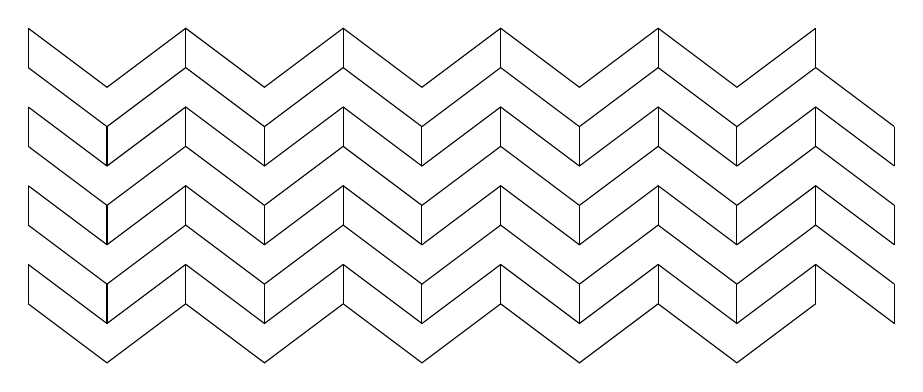
\begin{tikzpicture}[scale=1]


\draw  (0,0) -- (1,-0.75) -- (2,0) -- (3,-0.75) -- (4, 0) -- (5,-0.75)-- (6, 0) -- (7,-0.75)-- (8, 0) -- (9,-0.75)-- (10, 0);
\draw  (0,0.5) -- (1,-0.25) -- (2,0.5) -- (3,-0.25) -- (4, 0.5) -- (5,-0.25)-- (6, 0.5) -- (7,-0.25)-- (8, 0.5) -- (9,-0.25)-- (10, 0.5) -- (11,-0.25);
\draw  (0,1) -- (1,0.25) -- (2,1) -- (3,0.25) -- (4, 1) -- (5,0.25)-- (6, 1) -- (7,0.25)-- (8, 1) -- (9,0.25)-- (10, 1) -- (11,0.25);
\draw  (0,1.5) -- (1,0.75) -- (2,1.5) -- (3,0.75) -- (4, 1.5) -- (5,0.75)-- (6, 1.5) -- (7,0.75)-- (8, 1.5) -- (9,0.75)-- (10, 1.5) -- (11,0.75);
\draw  (0,2) -- (1,1.25) -- (2,2) -- (3,1.25) -- (4, 2) -- (5,1.25)-- (6, 2) -- (7,1.25)-- (8, 2) -- (9,1.25)-- (10, 2) -- (11,1.25);
\draw  (0,2.5) -- (1,1.75) -- (2,2.5) -- (3,1.75) -- (4, 2.5) -- (5,1.75)-- (6, 2.5) -- (7,1.75)-- (8, 2.5) -- (9,1.75)-- (10, 2.5) -- (11,1.75);
\draw  (0,3) -- (1,2.25) -- (2,3) -- (3,2.25) -- (4, 3) -- (5,2.25)-- (6, 3) -- (7,2.25)-- (8, 3) -- (9,2.25)-- (10, 3) -- (11,2.25);
\draw  (0,3.5) -- (1,2.75) -- (2,3.5) -- (3,2.75) -- (4, 3.5) -- (5,2.75)-- (6, 3.5) -- (7,2.75)-- (8,3.5) -- (9,2.75)-- (10, 3.5);


\draw (0,0) -- (0,0.5)   (0,1) -- (0,1.5)  (0,2) -- (0,2.5)  (0,3) -- (0,3.5);
\draw (2,0) -- (2,0.5)   (2,1) -- (2,1.5)  (2,2) -- (2,2.5)  (2,3) -- (2,3.5);
\draw (4,0) -- (4,0.5)   (4,1) -- (4,1.5)  (4,2) -- (4,2.5)  (4,3) -- (4,3.5);
\draw (6,0) -- (6,0.5)   (6,1) -- (6,1.5)  (6,2) -- (6,2.5)  (6,3) -- (6,3.5);
\draw (8,0) -- (8,0.5)   (8,1) -- (8,1.5)  (8,2) -- (8,2.5)  (8,3) -- (8,3.5);
\draw (10,0) -- (10,0.5)   (10,1) -- (10,1.5)  (10,2) -- (10,2.5)  (10,3) -- (10,3.5);

\draw (1,-0.25)  -- (1,0.25)  (1,0.75) -- (1,1.25) (1,1.75) -- (1,2.25);
\draw (3,-0.25) --  (3,0.25)  (3,0.75) -- (3,1.25) (3,1.75) -- (3,2.25);
\draw (5,-0.25)  -- (5,0.25)  (5,0.75) --  (5,1.25)  (5,1.75) -- (5,2.25);
\draw (7,-0.25) --  (7,0.25) (7,0.75)  --(7,1.25) (7,1.75) -- (7,2.25);
\draw (9,-0.25)  -- (9,0.25) (9,0.75) -- (9,1.25) (9,1.75)  --(9,2.25);
\draw (11,-0.25)  -- (11,0.25) (11,0.75) -- (11,1.25)  (11,1.75) -- (11,2.25);




\end{tikzpicture}
\end{center}
\caption{A wallpaper pattern in ${\mathbb R}^2$}
\label{Wallpaper}
\end{figure}
 
 
 
\subsection*{The Wallpaper Groups}
 
 
 
Suppose that we wish to study wallpaper patterns in the plane or
crystals in three dimensions. Wallpaper patterns are simply repeating
patterns in the plane (Figure~\ref{Wallpaper}). The analogs of
wallpaper patterns in ${\mathbb R}^3$ are crystals, which we can think of
as repeating patterns of molecules in three dimensions
(Figure~\ref{Crystals}). The mathematical equivalent of a wallpaper or
crystal pattern is called a  lattice. 
 
 
 
\begin{figure}[hbt]


%Replaced figure with tikz figure - TWJ 6/11/2010
\begin{center}
\tikzpreface{matrix_crystal_R3}
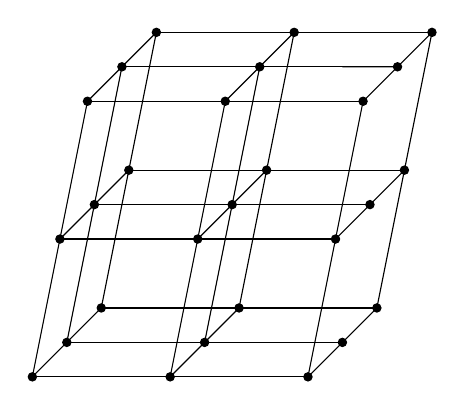
\begin{tikzpicture}[scale=1.75]


\draw  (0,0) -- (2,0)  (0.25,0.25) -- (2.25,0.25)  (0.5,0.5) -- (2.5,0.5);

\foreach \x in {0,1,2} \filldraw[fill=black, draw=black] (\x,0) circle (0.03);
\foreach \x in {0.25,1.25,2.25} \filldraw[fill=black, draw=black] (\x,0.25) circle (0.03);
\foreach \x in {0.5,1.5,2.5} \filldraw[fill=black, draw=black] (\x,0.5) circle (0.03);

\draw  (0.2,1) -- (2.2,1)  (0.45,1.25) -- (2.45,1.25)  (0.7,1.5) -- (2.7,1.5) ;

\foreach \x in {0.2,1.2,2.2} \filldraw[fill=black, draw=black] (\x,1) circle (0.03);
\foreach \x in {0.45,1.45,2.45} \filldraw[fill=black, draw=black] (\x,1.25) circle (0.03);
\foreach \x in {0.7,1.7,2.7} \filldraw[fill=black, draw=black] (\x,1.5) circle (0.03);

\draw  (0.4,2) -- (2.4,2)  (0.65,2.25) -- (2.65,2.25)  (0.9,2.5) -- (2.9,2.5) ;

\foreach \x in {0.4,1.4,2.4} \filldraw[fill=black, draw=black] (\x,2) circle (0.03);
\foreach \x in {0.65,1.65,2.65} \filldraw[fill=black, draw=black] (\x,2.25) circle (0.03);
\foreach \x in {0.9,1.9,2.9} \filldraw[fill=black, draw=black] (\x,2.5) circle (0.03);

\draw (0,0) -- (0.4,2)  (0.25,0.25) -- (0.65,2.25) (0.5,0.5) -- (0.9,2.5);
\draw (1,0) -- (1.4,2)  (1.25,0.25) -- (1.65,2.25) (1.5,0.5) -- (1.9,2.5);
\draw (2,0) -- (2.4,2)  (2.25,2.25) -- (2.65,2.25) (2.5,0.5) -- (2.9,2.5);

\draw (0,0) -- (0.5,0.5)  (1,0) -- (1.5,0.5)  (2,0) -- (2.5,0.5);

\draw  (0.2,1) -- (0.7,1.5)  (1.2,1) -- (1.7,1.5)  (2.2,1) -- (2.7,1.5);

\draw  (0.4,2) -- (0.9,2.5) (1.4,2) -- (1.9,2.5)   (2.4,2) -- (2.9,2.5);


\end{tikzpicture}
\end{center}
\caption{A crystal structure in ${\mathbb R}^3$}
\label{Crystals}
\end{figure}
 
 

Let us examine wallpaper patterns in the plane a
little more closely. Suppose that ${\mathbf x}$ and ${\mathbf y}$ are
linearly independent vectors in ${\mathbb R}^2$; that is, one vector
cannot be a scalar multiple of the other. A \boldemph{
lattice}\index{Lattice of points} of ${\mathbf x}$ and ${\mathbf y}$ is
the set of all linear combinations $m {\mathbf x} + n {\mathbf y}$, where
$m$ and $n$ are integers. The vectors ${\mathbf x}$ and ${\mathbf y}$ are
said to be a \boldemph{basis}\index{Basis of a lattice} for the lattice.
 
 
\begin{figure}[htb]


%Replaced figure with tikz figure - TWJ 6/11/2010
\begin{center}
\tikzpreface{matrix_lattice_R2}
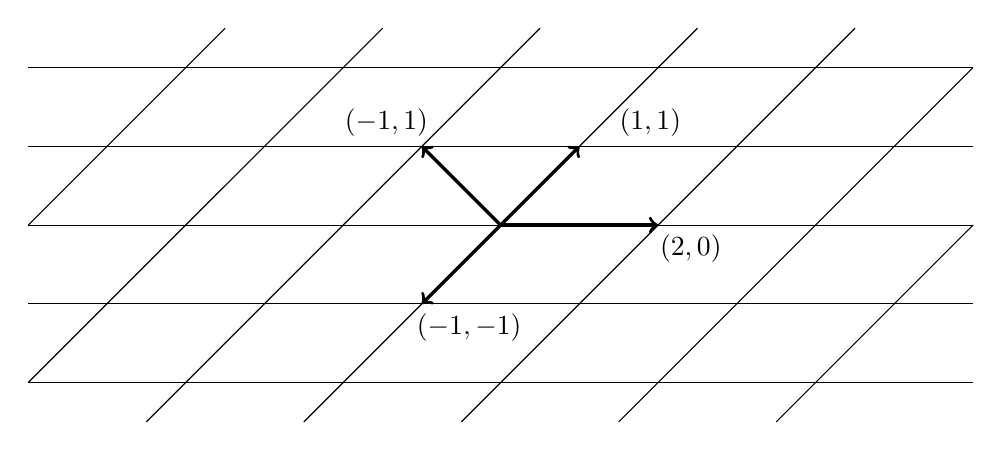
\begin{tikzpicture}[scale=1]



\foreach \x in {-2, -1, 0, 1, 2} \draw  (-6,\x) -- (6,\x); 

\draw (3.5,-2.5) -- (6,0);
\draw (1.5,-2.5) -- (6,2);
\draw (-0.5,-2.5) -- (4.5,2.5);
\draw (-2.5,-2.5) -- (2.5,2.5);
\draw (-4.5,-2.5) -- (0.5,2.5);
\draw (-6,-2) -- (-1.5,2.5);
\draw (-6,0) -- (-3.5,2.5);

\draw [->, very thick, black]  (0,0) -- (2,0);
\draw [->, very thick, black]  (0,0) -- (1,1);
\draw [->, very thick, black]  (0,0) -- (-1,1);
\draw [->, very thick, black]  (0,0) -- (-1,-1); 

\node [right] at (1.9,-0.3) {$(2,0)$};
\node [above] at (1.9,1) {$(1,1)$};
\node [above] at (-1.45,1) {$(-1,1)$};
\node [below] at (-0.4,-1) {$(-1,-1)$};

\end{tikzpicture}
\end{center}
\caption{A lattice in  ${\mathbb R}^2$}
\label{lattice}
\end{figure}
 
 
Notice that a lattice can have several bases. For example, the vectors
$(1,1)^{\rm t}$ and $(2,0)^{\rm t}$ have the  same lattice as the
vectors $(-1, 1)^{\rm t}$ and $(-1, -1)^{\rm t}$
(Figure~\ref{lattice}). However, any lattice is completely determined
by a basis. Given two bases for the same lattice, say $\{ {\mathbf x}_1,
{\mathbf x}_2 \}$ and $\{ {\mathbf y}_1, {\mathbf y}_2 \}$, we can write 
\begin{align*}
{\mathbf y}_1 & = \alpha_1  {\mathbf x}_1 + \alpha_2 {\mathbf x}_2 \\
{\mathbf y}_2 & = \beta_1  {\mathbf x}_1 + \beta_2 {\mathbf x}_2,
\end{align*}
where $\alpha_1$, $\alpha_2$, $\beta_1$, and $\beta_2$ are integers.
The matrix corresponding to this transformation is 
\[
U
=
\begin{pmatrix}
\alpha_1 & \alpha_2 \\
\beta_1 & \beta_2
\end{pmatrix}.
\]
If we wish to give ${\mathbf x}_1$ and ${\mathbf x}_2$ in terms of ${\mathbf
y}_1$ and ${\mathbf y}_2$, we need only calculate $U^{-1}$; that is, 
\[
U^{-1}
\begin{pmatrix}
{\mathbf y}_1 \\ {\mathbf y}_2
\end{pmatrix}
=
\begin{pmatrix}
{\mathbf x}_1 \\ {\mathbf x}_2
\end{pmatrix}.
\]
Since $U$ has integer entries, $U^{-1}$ must also have integer
entries; hence the determinants of both $U$ and $U^{-1}$ must be
integers. Because $U U^{-1} = I$,  
\[
\det(U U^{-1}) =\det(U) \det( U^{-1}) = 1;
\]
consequently, $\det(U) = \pm 1$. A matrix with determinant $\pm 1$ and
integer entries is called \boldemph{unimodular}\index{Matrix!unimodular}.
For example, the matrix 
\[
\begin{pmatrix}
3 & 1 \\
5 & 2
\end{pmatrix}
\]
is unimodular. It should be clear that there is a minimum length for
vectors in a lattice.  
 
 
We can classify lattices by studying their symmetry groups. The
symmetry group of a lattice is the subgroup of $E(2)$ that maps the
lattice to itself. We consider two lattices in ${\mathbb R}^2$ to be
equivalent if they have the same symmetry group.  Similarly,
classification of crystals in ${\mathbb R}^3$ is accomplished by
associating a symmetry group, called a \boldemph{space group}, with each
type of crystal\index{Group!space}. Two lattices are considered
different if their space groups are not the same.  The natural
question that now arises is how many space groups exist. 
 
 
A space group is composed of two parts: a \boldemph{translation
subgroup}\index{Subgroup!translation} and a \boldemph{point
group}\index{Group!point}.  The translation subgroup is an infinite
abelian subgroup of the space group made up of the translational
symmetries of the crystal; the point group is a finite group 
consisting  of rotations and reflections of the crystal about a point.
More specifically, a space group is a subgroup of $G \subset E(2)$
whose translations are a set of the form $\{ (I, t) : t \in L \}$,
where $L$ is a lattice. Space groups are, of course, infinite. Using
geometric arguments, we can prove the following theorem (see [5] or [6]).
 
 
 
 
\begin{theorem}
Every translation group in ${\mathbb R}^2$ is isomorphic to ${\mathbb Z}
\times {\mathbb Z}$.
\end{theorem}
 
 
\begin{figure}[bht]

\begin{center}
\tikzpreface{matrix_lattices_R2}
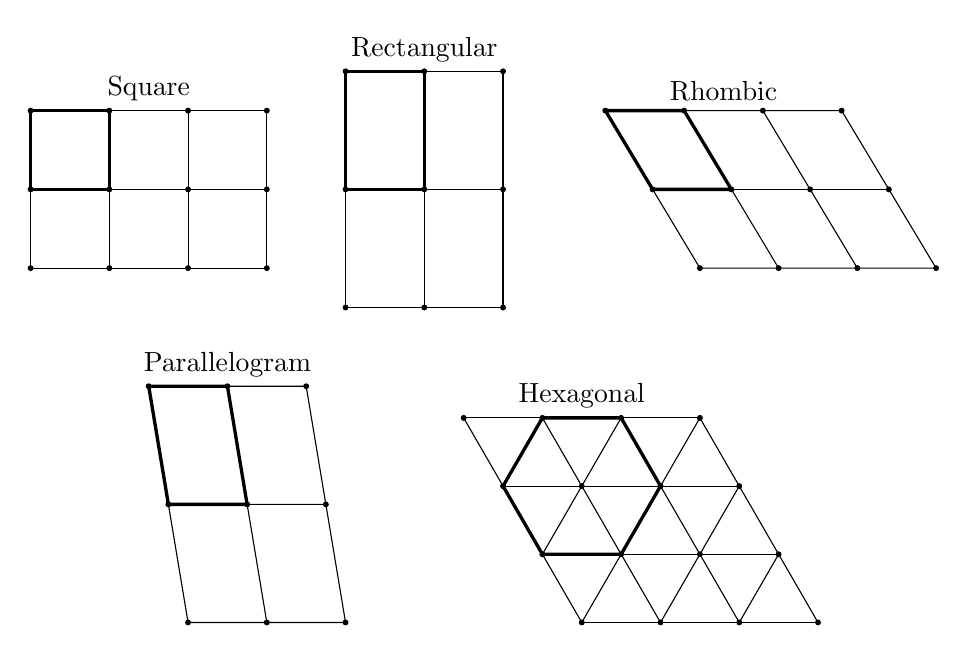
\begin{tikzpicture}[scale=1] %Replaced figure with tikz figure - TWJ 6/14/2010

\node [above] at (0,7) {Rectangular};
\draw (-1,4) -- (1,4) -- (1,7) -- (-1,7) -- cycle;
\draw  (0,4) -- (0,7)  (-1,5.5) -- (1,5.5);
\draw [very thick] (-1,5.5) -- (-1,7) -- (0,7) -- (0,5.5) -- cycle;
\foreach \x in {-1,0,1} \filldraw[fill=black, draw=black] (\x,4) circle (0.03);
\foreach \x in {-1,0,1} \filldraw[fill=black, draw=black] (\x,5.5) circle (0.03);
\foreach \x in {-1,0,1} \filldraw[fill=black, draw=black] (\x,7) circle (0.03);

\node [above] at (-3.5,6.5) {Square};
\draw (-2,4.5) -- (-5,4.5) -- (-5,6.5) -- (-2,6.5) -- cycle;
\draw  (-2,5.5) -- (-5,5.5)  (-3,4.5) -- (-3,6.5) (-4,4.5) -- (-4,6.5);
\draw [very thick] (-5,5.5) -- (-5,6.5) -- (-4,6.5) -- (-4,5.5) -- cycle;
\foreach \x in {-2, -3, -4, -5} \filldraw[fill=black, draw=black] (\x,4.5) circle (0.03);
\foreach \x in {-2, -3, -4, -5} \filldraw[fill=black, draw=black] (\x,5.5) circle (0.03);
\foreach \x in {-2, -3, -4, -5} \filldraw[fill=black, draw=black] (\x,6.5) circle (0.03);

\node [above] at (3.8,6.5) {Rhombic};
\draw (3.5,4.5)   -- (6.5,4.5) -- (5.3,6.5) -- (2.3,6.5) -- cycle;
\draw (2.9,5.5) -- (5.9,5.5);
\draw (4.5,4.5) -- (3.3,6.5);
\draw  (5.5,4.5) -- (4.3,6.5);
\draw [very thick] (2.3,6.5) -- (3.3,6.5) -- (3.9,5.5) -- (2.9,5.5) -- cycle;
\foreach \x in {3.5,4.5,5.5,6.5} \filldraw[fill=black, draw=black] (\x,4.5) circle (0.03);
\foreach \x in {2.9,3.9,4.9,5.9} \filldraw[fill=black, draw=black] (\x,5.5) circle (0.03);
\foreach \x in {2.3,3.3,4.3,5.3} \filldraw[fill=black, draw=black] (\x,6.5) circle (0.03);

\node [above] at (-2.5,3) {Parallelogram};
\draw (-1,0) -- (-3,0) -- (-3.5,3) -- (-1.5,3) -- cycle;
\draw  (-2,0) -- (-2.5,3)  (-3.25,1.5) -- (-1.25,1.5);
\draw [very thick] (-3.25,1.5) -- (-3.5,3) -- (-2.5,3) -- (-2.25,1.5) -- cycle;
\foreach \x in {-1,-2,-3} \filldraw[fill=black, draw=black] (\x,0) circle (0.03);
\foreach \x in {-1.25,-2.25,-3.25} \filldraw[fill=black, draw=black] (\x,1.5) circle (0.03);
\foreach \x in {-1.5,-2.5,-3.5} \filldraw[fill=black, draw=black] (\x,3) circle (0.03);

\node [above] at (2,2.6) {Hexagonal}; %Couldn't figure out an elegant way to do the hexagonal lattice - TWJ 6/14/2010
\draw (2,0) -- (5,0);
\draw (1.5,0.866) -- (4.5,0.866);
\draw (1,1.732) -- (4,1.732);
\draw (0.5,2.598) -- (3.5,2.598);
\draw (2,0) -- (0.5,2.598);
\draw (3,0) -- (1.5,2.598);
\draw (4,0) -- (2.5,2.598);
\draw (5,0) -- (3.5,2.598);
\draw (2,0) -- (3.5,2.598);
\draw (3,0) -- (4,1.732);
\draw (4,0) -- (4.5,0.866);
\draw (1.5,0.866) -- (2.5,2.598);
\draw (1,1.732) -- (1.5,2.598);
\draw [very thick] (1.5,0.866) -- (1,1.732) -- (1.5,2.598) -- (2.5,2.598) -- (3,1.732) --  (2.5,0.866) -- cycle;
\foreach \x in {2,3,4,5} \filldraw[fill=black, draw=black] (\x,0) circle (0.03);
\foreach \x in {1.5,2.5,3.5,4.5} \filldraw[fill=black, draw=black] (\x,0.866) circle (0.03);
\foreach \x in {1,2,3,4} \filldraw[fill=black, draw=black] (\x,1.732) circle (0.03);
\foreach \x in {0.5, 1.5,2.5,3.5} \filldraw[fill=black, draw=black] (\x,2.598) circle (0.03);

\end{tikzpicture}
\end{center}
\caption{Types of lattices in  ${\mathbb R}^2$}
\label{Types}
\end{figure}
 
 
The point group of $G$ is $G_0 = \{A : (A,b) \in G \text{ for some }
b \}$. In particular, $G_0$ must be a subgroup of $O(2)$. Suppose
that ${\mathbf x}$ is a vector in a lattice $L$ with space group $G$,
translation group $H$, and point group $G_0$. For any element $(A,
{\mathbf y})$ in $G$,   
\begin{align*}
(A, {\mathbf y}) (I, {\mathbf x}) (A, {\mathbf y})^{-1}
& =
(A,A {\mathbf x} + {\mathbf y}) (A^{-1},-A^{-1} {\mathbf y}) \\
& =
(A A^{-1},-A A^{-1} {\mathbf y} + A {\mathbf x} + {\mathbf y}) \\
& =
(I, A {\mathbf x});
\end{align*}
hence, $(I, A {\mathbf x})$ is in the translation group of $G$. More
specifically, $A {\mathbf x}$ must be in the lattice $L$. It is
important to note that $G_0$ is not usually a subgroup of the space
group $G$; however, if $T$ is the translation subgroup of $G$, then
$G/T \cong G_0$. The proof of the following theorem can be found in
[2], [5], or~[6].
 
 
 
\begin{theorem}
The point group in the wallpaper groups is isomorphic to ${\mathbb Z}_n$
or $D_n$, where $n = 1, 2, 3, 4, 6$. 
\end{theorem}
 
 
To answer the question of how the point groups and the translation
groups can be combined, we must look at the different types of
lattices. Lattices can be classified by the structure of a single
lattice cell. The possible cell shapes are parallelogram, rectangular,
square, rhombic, and hexagonal (Figure~\ref{Types}). The wallpaper
groups can now be classified according to the types of reflections
that occur in each group: these are ordinarily reflections, glide
reflections, both, or none.
 
 
 
\begin{table}[htb]
\caption{The 17 wallpaper groups}{\small
\begin{center}
\begin{tabular}{|l|l|l|l|}
\hline
Notation and &             &              & Reflections  \\
Space Groups & Point Group & Lattice Type & or Glide Reflections? \\
\hline
p1 & ${\mathbb Z}_1$ & parallelogram & none \\
p2 & ${\mathbb Z}_2$ & parallelogram & none \\
p3 & ${\mathbb Z}_3$ & hexagonal & none \\
p4 & ${\mathbb Z}_4$ & square & none \\
p6 & ${\mathbb Z}_6$ & hexagonal & none \\
pm & $D_1$ & rectangular & reflections \\
pg & $D_1$ & rectangular & glide reflections\\
cm & $D_1$ & rhombic & both \\
pmm & $D_2$ & rectangular & reflections \\
pmg & $D_2$ & rectangular & glide reflections \\
pgg & $D_2$ & rectangular & both \\
c2mm & $D_2$ & rhombic & both \\
p3m1, p31m & $D_3$ & hexagonal & both \\
p4m, p4g & $D_4$ & square & both \\
p6m & $D_6$ & hexagonal & both \\
\hline
\end{tabular} \label{table:wallpaper}
\end{center}
}
\end{table}
 
 
\begin{theorem}
There are exactly 17 wallpaper groups.
\end{theorem}
 
 
\begin{figure}[htb]


\begin{center}
\tikzpreface{matrix_p4m_p4g}
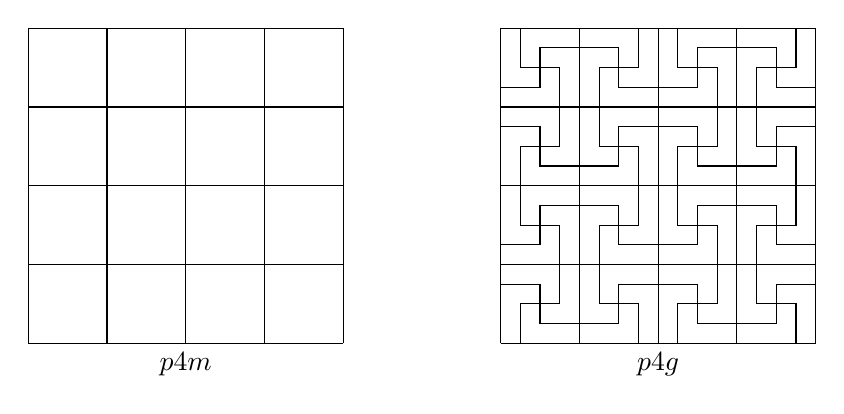
\begin{tikzpicture}[scale=1] %Replaced figure with tikz figure - TWJ 6/14/2010

\draw[step=1] (-5,0) grid (-1,4);
\node [below] at (-3,0) {$p4m$};

\draw[step=1] (1,0) grid (5,4);
\node [below] at (3,0) {$p4g$};
\draw (1.25,0) -- (1.25,0.5) -- (1.75,0.5) -- (1.75,1.5) -- (1.25,1.5) -- (1.25,2.5) -- (1.75,2.5) -- (1.75,3.5) -- (1.25,3.5) -- (1.25,4);
\draw  (2.75,0) -- (2.75,0.5) -- (2.25,0.5) -- (2.25,1.5) -- (2.75,1.5) -- (2.75,2.5) -- (2.25,2.5) -- (2.25,3.5) -- (2.75,3.5) -- (2.75,4);
\draw   (3.25,0) -- (3.25,0.5) -- (3.75,0.5) -- (3.75,1.5) -- (3.25,1.5) -- (3.25,2.5) -- (3.75,2.5) -- (3.75,3.5) -- (3.25,3.5) -- (3.25,4);
\draw   (4.75,0) -- (4.75,0.5) -- (4.25,0.5) -- (4.25,1.5) -- (4.75,1.5) -- (4.75,2.5) -- (4.25,2.5) -- (4.25,3.5) -- (4.75,3.5) -- (4.75,4);

\draw  (1,0.75) -- (1.5,0.75) -- (1.5,0.25) -- (2.5,0.25) -- (2.5,0.75) -- (3.5,0.75) -- (3.5,0.25) -- (4.5,0.25) -- (4.5,0.75) -- (5, 0.75);
\draw  (1,1.25) -- (1.5,1.25) -- (1.5,1.75) -- (2.5,1.75) -- (2.5,1.25) -- (3.5,1.25) -- (3.5,1.75) -- (4.5,1.75) -- (4.5,1.25) -- (5, 1.25);

\draw  (1,2.75) -- (1.5,2.75) -- (1.5,2.25) -- (2.5,2.25) -- (2.5,2.75) -- (3.5,2.75) -- (3.5,2.25) -- (4.5,2.25) -- (4.5,2.75) -- (5, 2.75);
\draw (1,3.25) -- (1.5,3.25) -- (1.5,3.75) -- (2.5,3.75) -- (2.5,3.25) -- (3.5,3.25) -- (3.5,3.75) -- (4.5,3.75) -- (4.5,3.25) -- (5, 3.25);


\end{tikzpicture}
\end{center}
\caption{The wallpaper groups p4m and  p4g}
\label{p4m}
\end{figure}
 
 
 
The 17 wallpaper groups are listed in Table~\ref{table:wallpaper}. The groups p3m1 and
p31m can be distinguished by whether or not all of their threefold
centers lie on the reflection axes: those of p3m1 must, whereas those
of p31m may not. Similarly, the fourfold centers of p4m must lie on
the reflection axes whereas those of p4g need not (Figure~\ref{p4m}).
The complete proof of this theorem can be found in several of the
references at the end of this chapter, including [5], [6], [10],
and~[11]. 
 
 
 
\histhead
 
 
\noindent{\small \histf
Symmetry groups have intrigued mathematicians for a long time.
Leonardo da Vinci was probably the first person to know all of the
point groups.  At the International Congress of Mathematicians in
1900, David Hilbert\index{Hilbert, David} gave a now-famous address
outlining 23 problems to guide mathematics in the twentieth
century.  Hilbert's eighteenth problem asked whether or not
crystallographic groups in $n$ dimensions were always finite.  In
1910, L.~Bieberbach\index{Bieberbach, L.} proved that crystallographic
groups are finite in every dimension.  Finding out how many of these
groups there are in each dimension is another matter. In ${\mathbb R}^3$
there are 230 different space groups; in ${\mathbb R}^4$ there are 4783.
No one has been able to compute the number of space groups for ${\mathbb
R}^5$ and beyond. It is interesting to note that the crystallographic
groups were found mathematically for ${\mathbb R}^3$ before the 230
different types of crystals were actually discovered in nature.
\histbox
}
 
 
 
\markright{EXERCISES}
\section*{Exercises}
\exrule
 
 
{\small
\begin{enumerate}
 
 
 
\item
Prove the identity
\[
\langle {\mathbf x}, {\mathbf y} \rangle = \frac{1}{2}
\left[
\|{\mathbf x} + {\mathbf y}\|^2 - \|{\mathbf x}\|^2 - \| {\mathbf y}\|^2
\right].
\]
 
 
\item
Show that $O(n)$ is a group.
 
 
\item
Prove that the following matrices are orthogonal. Are any of
these matrices in $SO(n)$?
\begin{multicols}{2}
\begin{enumerate}

\item
\[
\begin{pmatrix}
1/\sqrt{2} & -1/\sqrt{2} \\
1/\sqrt{2} & 1/\sqrt{2}
\end{pmatrix}
\]

\item
\[
\begin{pmatrix}
1 / \sqrt{5} & 2 / \sqrt{5} \\
- 2 /\sqrt{5} & 1/ \sqrt{5}
\end{pmatrix}
\]

\item
\[
\begin{pmatrix}
4/ \sqrt{5} & 0 & 3 / \sqrt{5} \\
-3 / \sqrt{5} & 0 & 4 / \sqrt{5} \\
0 & -1 & 0
\end{pmatrix}
\]

\item
\[
\begin{pmatrix}
1/3 & 2/3 & - 2/3 \\
- 2/3 & 2/3 & 1/3 \\
-2/3 & 1/3 & 2/3
\end{pmatrix}
\]


\end{enumerate}
\end{multicols}
 

 
\item %%%%%%%%%%%%%%%%%%%%%%
Determine the symmetry group of each of the figures in
Figure~\ref{Determine}. 
\begin{figure}[htb]

\begin{center}
\tikzpreface{matrix_group_exercise}
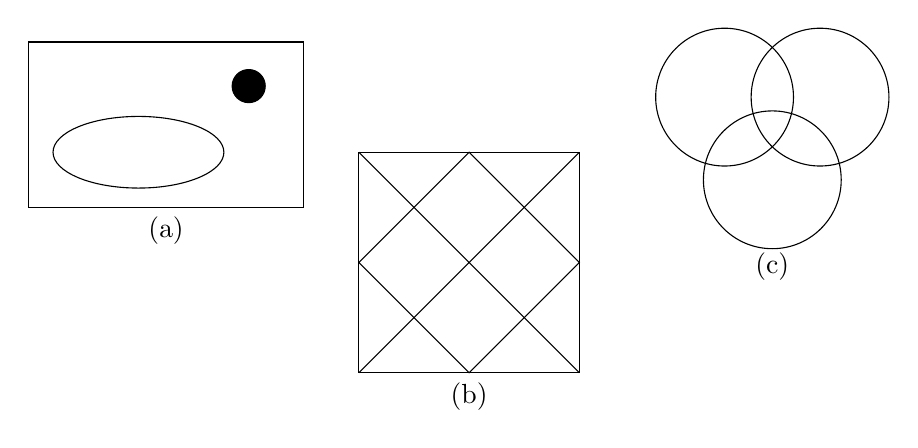
\begin{tikzpicture}[scale=0.7] %Replaced figure with tikz figure - TWJ 6/14/2010

\draw (-2,0) -- (2,0) -- (2,4) -- (-2,4) -- cycle;
\draw (0,0) -- (2,2) -- (0,4) -- (-2,2) -- cycle;
\draw (-2,0) -- (2,4) (2,0) -- (-2,4);
\node [below] at (0,0) {(b)};

\draw (-3,3) -- (-8,3) -- (-8,6) -- (-3,6) -- cycle;
\draw (-6,4) ellipse (1.55 and 0.65);
\filldraw[fill=black, draw=black] (-4,5.2) circle (0.3);
\node [below] at (-5.5,3) {(a)};



\draw (5.5,4.5)  +(270:1) circle (1.25);
\draw (5.5,4.5)  +(30:1) circle (1.25);
\draw (5.5,4.5)  +(150:1) circle (1.25);
\node [below] at (5.5,2.35) {(c)};


\end{tikzpicture}
\end{center}
\caption{}
\label{Determine}
\end{figure}
 
 
\item
Let ${\mathbf x}$, ${\mathbf y}$, and ${\mathbf w}$ be vectors in ${\mathbb
R}^n$ and $\alpha \in {\mathbb R}$.  Prove each of the following
properties of inner products.
\begin{enumerate}
 
 \item
$\langle {\mathbf x}, {\mathbf y} \rangle = \langle {\mathbf y}, {\mathbf x}
\rangle$. 
 
 \item
$\langle {\mathbf x}, {\mathbf y} + {\mathbf w} \rangle = \langle
{\mathbf x}, {\mathbf y} \rangle + \langle {\mathbf x}, {\mathbf w}
\rangle$.
 
 \item
$\langle \alpha {\mathbf x}, {\mathbf y} \rangle = \langle
{\mathbf x}, \alpha {\mathbf y} \rangle = \alpha \langle  {\mathbf
x}, {\mathbf y} \rangle$.
 
 \item
$\langle {\mathbf x}, {\mathbf x} \rangle \geq 0$ with equality exactly
when ${\mathbf x} = 0$. 
 
 \item
If $\langle {\mathbf x}, {\mathbf y} \rangle = 0$  for all ${\mathbf x}$ in
${\mathbb R}^n$, then ${\mathbf y} = 0$. 
 
\end{enumerate}
 
 
\item \label{matrix:En_group_exercise}
Verify that
\[
E(n)
=
\{(A, {\mathbf x}) : A \in O(n) \mbox{ and } {\mathbf x} \in
{\mathbb R}^n \}
\]
is a group.
 
 
\item
Prove that $\{ (2,1), (1,1) \}$  and $\{ ( 12, 5), ( 7, 3) \}$ are bases
for the same lattice. 
 
 
\item
Let $G$ be a subgroup of $E(2)$ and suppose that $T$ is the
translation subgroup of $G$.  Prove that the point group of $G$ is
isomorphic to $G/T$. 
 
 
\item
Let $A \in SL_2({\mathbb R})$ and suppose that the vectors ${\mathbf x}$
and ${\mathbf y}$ form two sides of a parallelogram in ${\mathbb R}^2$.
Prove that the area of this parallelogram is the same as the area of
the parallelogram with sides $A{\mathbf x}$ and $A{\mathbf y}$. 
 
 
\item
Prove that $SO(n)$ is a normal subgroup of $O(n)$.
 
 
\item
Show that any isometry $f$ in ${\mathbb R}^n$ is a one-to-one map.
 
 
\item
Show that an element in $E(2)$ of the form $(A, {\mathbf x})$,
where ${\mathbf x} \neq 0$, has infinite order.
 
 
\item
Prove or disprove: There exists an infinite abelian subgroup of 
$O(n)$.
 
 
\item
Let ${\mathbf x} = (x_1, x_2)$ be a point on the unit circle in ${\mathbb
R}^2$; that is, $x_1^2 + x_2^2 = 1$. If $A \in O(2)$, show that $A
{\mathbf x}$ is also a point on the unit circle. 
 
 
 
\item
Let $G$ be a group with a subgroup $H$ (not necessarily normal) and a
normal subgroup $N$. Then $G$ is a \boldemph{semidirect
product}\index{Semidirect product} of $N$ by $H$ if  
\begin{itemize}
 
 \item
$H \cap N = \{ id \}$;
 
 \item
$HN=G$.
 
\end{itemize}
Show that each of the following is true.
\begin{enumerate}
 
 \item
$S_3$ is the semidirect product of $A_3$ by $H = \{(1), (12) \}$.
 
 \item
The quaternion group, $Q_8$, cannot be written as a semidirect product. 
 
 \item
$E(2)$ is the semidirect product of $O(2)$ by $H$, where $H$ consists
of all translations in ${\mathbb R}^2$. 
 
\end{enumerate}
 
 
 
\item
Determine which of the 17 wallpaper groups preserves the symmetry of
the pattern in Figure~\ref{Wallpaper}.  
 
\begin{figure}[htb]

\begin{center}
\tikzpreface{matrix_wallpaper_exercise}
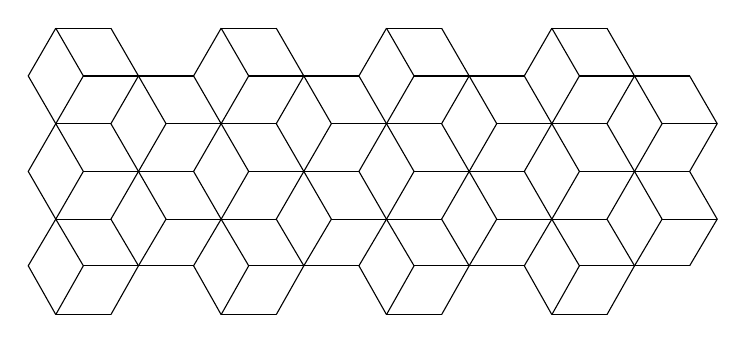
\begin{tikzpicture}[scale=0.7] %Replaced figure with tikz figure - TWJ 6/14/2010

\draw (0.5,0) -- (1.5,0)  (3.5,0) -- (4.5,0) (6.5,0) -- (7.5,0) (9.5,0) -- (10.5,0);
\draw (1,0.886) -- (3,0.886) (4,0.886) -- (6,0.886) (7,0.886) -- (9,0.886) (10,0.886) -- (12,0.886);
\draw (0.5,1.732) -- (1.5,1.732)  (2.5,1.732) -- (4.5,1.732) (5.5,1.732) -- (7.5,1.732) (8.5,1.732) -- (10.5,1.732) (11.5,1.732) -- (12.5,1.732);
\draw (1,2.598) -- (3,2.598) (4,2.598) -- (6,2.598) (7,2.598) -- (9,2.598) (10,2.598) -- (12,2.598);
\draw (0.5,3.464) -- (1.5,3.464)  (2.5,3.464) -- (4.5,3.464) (5.5,3.464) -- (7.5,3.464) (8.5,3.464) -- (10.5,3.464) (11.5,3.464) -- (12.5,3.464);
\draw (1,4.33) -- (3,4.33) (4,4.33) -- (6,4.33) (7,4.33) -- (9,4.33) (10,4.33) -- (12,4.33);
\draw (0.5,5.196) -- (1.5,5.196)  (3.5,5.196) -- (4.5,5.196) (6.5,5.196) -- (7.5,5.196) (9.5,5.196) -- (10.5,5.196);

\draw (0.5,0) -- (0,0.886) -- (0.5,1.732) -- (0,2.598) -- (0.5,3.464) -- (0,4.33) -- (0.5,5.196);
\draw (0.5,0) -- (1,0.886) -- (0.5,1.732) -- (1,2.598) -- (0.5,3.464) -- (1,4.33) -- (0.5,5.196);
\draw (1.5,0) -- (2,0.886) -- (1.5,1.732) -- (2,2.598) -- (1.5,3.464) -- (2,4.33) -- (1.5,5.196);
\draw (2,0.886) -- (2.5,1.732) -- (2,2.598) -- (2.5,3.464) -- (2,4.33);
\draw (3,0.886) -- (3.5,1.732) -- (3,2.598) -- (3.5,3.464) -- (3,4.33);
\draw (3.5,0) -- (3,0.886) (3,4.33) -- (3.5,5.196);
\draw (3.5,0) -- (4,0.886) -- (3.5,1.732) -- (4,2.598) -- (3.5,3.464) -- (4,4.33) -- (3.5,5.196);
\draw (4.5,0) -- (5,0.886) -- (4.5,1.732) -- (5,2.598) -- (4.5,3.464) -- (5,4.33) -- (4.5,5.196);
\draw (5,0.886) -- (5.5,1.732) -- (5,2.598) -- (5.5,3.464) -- (5,4.33);
\draw (6.5,0) -- (6,0.886) -- (6.5,1.732) -- (6,2.598) -- (6.5,3.464) -- (6,4.33) -- (6.5,5.196);
\draw (6.5,0) -- (7,0.886) -- (6.5,1.732) -- (7,2.598) -- (6.5,3.464) -- (7,4.33) -- (6.5,5.196);
\draw (7.5,0) -- (8,0.886) -- (7.5,1.732) -- (8,2.598) -- (7.5,3.464) -- (8,4.33) -- (7.5,5.196);
\draw (8,0.886) -- (8.5,1.732) -- (8,2.598) -- (8.5,3.464) -- (8,4.33);
\draw (9.5,0) -- (9,0.886) -- (9.5,1.732) -- (9,2.598) -- (9.5,3.464) -- (9,4.33) -- (9.5,5.196);
\draw (9.5,0) -- (10,0.886) -- (9.5,1.732) -- (10,2.598) -- (9.5,3.464) -- (10,4.33) -- (9.5,5.196);
\draw (10.5,0) -- (11,0.886) -- (10.5,1.732) -- (11,2.598) -- (10.5,3.464) -- (11,4.33) -- (10.5,5.196);
\draw (11,0.886) -- (11.5,1.732) -- (11,2.598) -- (11.5,3.464) -- (11,4.33);
\draw (12,0.886) -- (12.5,1.732) -- (12,2.598) -- (12.5,3.464) -- (12,4.33);



\end{tikzpicture}
\end{center}
\caption{}
\label{For17}
\end{figure}
 
\item
Determine which of the 17 wallpaper groups preserves the symmetry of
the pattern in Figure~\ref{For17}.  
 
 
 
\item
Find the rotation group of a dodecahedron.
 
  
 
\item
For each of the 17 wallpaper groups, draw a wallpaper pattern having
that group as a symmetry group.  
 
\end{enumerate}
}
 
 
 
\subsection*{References and Suggested Readings}
 
 
 
{\small
\begin{itemize} %%References checked -- TWJ 6/14/2010
 
\item[\textbf{[1]}]
Coxeter, H. M. and Moser, W. O. J. \textit{Generators and
Relations for Discrete Groups}, 3rd ed. Springer-Verlag, New
York, 1972.
 
\item[\textbf{[2]}]
Grove, L. C. and Benson, C. T. \textit{Finite Reflection
Groups}. 2nd ed. Springer-Verlag, New York, 1985.
 
\item[\textbf{[3]}]
Hiller, H. ``Crystallography and Cohomology of Groups,''
\textit{American Mathematical Monthly} \textbf{93} (1986), 765--79.
 
\item[\textbf{[4]}]
Lockwood, E. H. and Macmillan, R. H. \textit{Geometric
Symmetry}. Cambridge University Press, Cambridge, 1978.
 
\item[\textbf{[5]}]
Mackiw, G. \textit{Applications of Abstract Algebra}. Wiley,
New York, 1985.
 
 
\item[\textbf{[6]}]
Martin,  G.  \textit{Transformation  Groups:  An Introduction to
Symmetry}.  Springer-Verlag, New York, 1982.
 
  
\item[\textbf{[7]}]
Milnor, J. ``Hilbert's Problem 18: On Crystallographic
Groups, Fundamental Domains, and Sphere Packing,'' {\it
Proceedings of Symposia in Pure Mathematics} \textbf{18},
American Mathematical Society, 1976.
 
\item[\textbf{[8]}]
Phillips, F. C. \textit{An Introduction to Crystallography}.
4th ed. Wiley, New York, 1971.
 
\item[\textbf{[9]}]
Rose, B. I. and Stafford, R. D. ``An Elementary Course in
Mathematical Symmetry,'' \textit{American Mathematical Monthly} \textbf{
88} (1980), 54--64.
 
 
\item[\textbf{[10]}]
Schattschneider, D. ``The Plane Symmetry Groups: Their
Recognition and Their Notation,'' \textit{American Mathematical 
Monthly} \textbf{85} (1978), 439--50.
 
 
\item[\textbf{[11]}]
Schwarzenberger, R. L. ``The 17 Plane Symmetry Groups,'' {\it
Mathematical  Gazette} \textbf{58} (1974), 123--31. 
 
 
\item[\textbf{[12]}]
Weyl, H. \textit{Symmetry}. Princeton University Press, Princeton, NJ,
1952. 
 
 
\end{itemize}
}
 
 
 
 
   %Groups of Symmetries
%%%%(c)
%%%%(c)  This file is a portion of the source for the textbook
%%%%(c)
%%%%(c)    Abstract Algebra: Theory and Applications
%%%%(c)    by Thomas W. Judson
%%%%(c)
%%%%(c)    Sage Material
%%%%(c)    Copyright 2011 by Robert A. Beezer
%%%%(c)
%%%%(c)  See the file COPYING.txt for copying conditions
%%%%(c)
%%%%(c)
There are no exercises for this section.   %Abelian and Solvable Groups
% !TEX root = aata.tex
%%%%(c)
%%%%(c)  This file is a portion of the source for the textbook
%%%%(c)
%%%%(c)    Abstract Algebra: Theory and Applications
%%%%(c)    Copyright 1997 by Thomas W. Judson
%%%%(c)
%%%%(c)  See the file COPYING.txt for copying conditions
%%%%(c)
%%%%(c)
\chap{Group Actions}{actions}

Group actions generalize group multiplication.  If $G$ is a group and $X$ is an arbitrary set, a group action of an element $g \in G$ and $x \in X$ is a product, $gx$,  living in $X$.  Many problems in algebra may best be attacked via group actions.  For example, the proofs of the Sylow theorems and of Burnside's Counting Theorem are most easily understood when they are formulated in terms of group actions. 


\section{Groups Acting on Sets}

Let $X$ be a set and $G$ be a group.  A  \boldemph{(left) action}\index{Group!action} of $G$ on $X$ is a map $G \times X \rightarrow X$ given by $(g,x) \mapsto gx$, where 
\begin{enumerate}
 
\item 
$ex = x$ for all $x \in X$;
 
\item 
$(g_1 g_2)x = g_1(g_2 x)$ for all $x \in X$ and all $g_1, g_2 \in G$. 
 
\end{enumerate}
Under these considerations $X$ is called a \boldemph{$G$-set}\index{$G$-set}.  Notice that we are not requiring $X$ to be related to $G$ in any way.  It is true that every group $G$ acts on every set $X$ by the trivial action $(g,x) \mapsto x$; however, group actions are more interesting if the set $X$ is somehow related to the group $G$. 

\begin{example}{GL2_action}
Let $G = GL_2( {\mathbb R} )$ and $X = {\mathbb R}^2$. Then $G$ acts on $X$ by left multiplication.  If $v \in {\mathbb R}^2$ and $I$ is the identity matrix, then $Iv = v$.  If $A$ and $B$ are $2 \times 2$ invertible matrices, then $(AB)v = A(Bv)$ since matrix multiplication is
associative. 
\end{example}

\begin{example}{D4_action}
Let $G = D_4$ be the symmetry group of a square.  If $X = \{ 1, 2, 3, 4 \}$ is the set of vertices of the square, then we can consider $D_4$
to consist of the following permutations: 
\[
\{ (1), (13), (24), (1432), (1234), (12)(34), (14)(23), (13)(24) \}.
\]
The elements of $D_4$ act on $X$ as functions.  The permutation $(13)(24)$ acts on vertex 1 by sending it to vertex 3, on vertex 2 by
sending it to vertex 4, and so on.  It is easy to see that the  axioms of a group action are satisfied.
\mbox{\hspace{1in}}
\end{example}



In general, if $X$ is any set and $G$ is a subgroup of $S_X$, the
group of all permutations acting on $X$, then $X$ is a $G$-set under
the group action 
\[
(\sigma, x) \mapsto \sigma(x)
\]
for $\sigma \in G$ and $x \in X$.
 
 
\begin{example}{left_action}
If we let $X = G$, then every group $G$ acts on itself by the left
regular representation; that is, $(g,x) \mapsto \lambda_g(x) = gx$, 
where  $\lambda_g$ is left multiplication:
\begin{gather*}
e \cdot x = \lambda_e x = ex = x \\
(gh) \cdot x = \lambda_{gh}x = \lambda_g \lambda_h x =
\lambda_g(hx) = g \cdot ( h \cdot x).
\end{gather*}
If $H$ is a subgroup of $G$, then $G$ is an $H$-set under left
multiplication by elements of $H$. 
\end{example}
 
 
\begin{example}{conj_action}
Let $G$ be a group and suppose that $X=G$. If $H$ is a subgroup of
$G$, then $G$ is an $H$-set under \boldemph{
conjugation}\index{Conjugation}; that is, we can define an action of
$H$ on $G$, 
\[
H \times G \rightarrow G,
\]
via
\[
(h,g) \mapsto hgh^{-1}
\]
for $h \in H$ and $g \in G$.  Clearly, the first axiom for a group
action holds.  Observing that 
\begin{align*}
(h_1 h_2, g) 
& = h_1 h_2 g (h_1 h_2 )^{-1} \\
& = h_1( h_2 g h_2^{-1}) h_1^{-1} \\
& =  (h_1, (h_2, g) ),
\end{align*}
we see that the second condition is also satisfied.
\end{example}
 
 
\begin{example}{left_coset_action}
Let $H$ be a subgroup of $G$ and ${\mathcal L}_H$ the set of left cosets
of $H$.  The set ${\mathcal L}_H$ is a $G$-set under the action
\[
(g, xH) \mapsto gxH.
\]
Again, it is easy to see that the first axiom is true. Since $(g g')xH
= g( g'x H)$, the second axiom is  also true.
\end{example}
 
 
 
If $G$ acts on a set $X$ and $x, y \in X$, then $x$ is said to be
\boldemph{$G$-equivalent}\index{$G$-equivalent} to $y$ if there exists a
$g \in G$ such that $gx =y$. We  write $x \sim_G y$ or $x \sim y$ if
two elements are $G$-equivalent. 
 
 
\begin{proposition}
Let  $X$ be a $G$-set. Then $G$-equivalence is an equivalence relation
on $X$. 
\end{proposition}
 
 
\begin{proof}
The relation $\sim$ is reflexive since $ex = x$. Suppose that $x \sim
y$ for $x, y \in X$. Then there exists a $g$ such that $gx = y$. In
this case $g^{-1}y=x$; hence, $y \sim x$. To show that the relation is
transitive, suppose that $x \sim y$ and $y \sim z$. Then there must
exist group elements $g$ and $h$ such that $gx = y$ and $hy= z$. So $z
= hy = (hg)x$, and  $x$ is equivalent to $z$.
\end{proof}
 
 
\medskip
 
 
If $X$ is a $G$-set, then each partition of $X$ associated with
$G$-equivalence is called an \boldemph{orbit}\index{Orbit} of $X$ under
$G$.  We will denote the orbit that contains an element $x$  of $X$ by
${\mathcal O}_x$\label{noteorbit}. 
 
 
\begin{example}{permute_action}
Let $G$ be the permutation group defined by
\[
G =\{(1), (1 2
3), (1 3 2), (4 5), (1 2 3)(4 5), (1 3 2)(4 5) \}
\]
and $X = \{ 1, 2, 3, 4, 5\}$. Then $X$ is a $G$-set. The orbits are
${\mathcal O}_1 = {\mathcal O}_2 = {\mathcal O}_3 =\{1, 2, 3\}$ and $ {\mathcal O}_4=
{\mathcal O}_5 = \{4, 5\}$. 
\end{example}
 
 

 
 
Now suppose that $G$ is a group acting on a set $X$ and let $g$ be
an element of $G$. The \boldemph{fixed point set}\index{Fixed point
set} of $g$ in $X$, denoted by $X_g$\label{notefixed}, is the set of 
all $x \in X$ such
that $gx = x$.  We can also study the group elements $g$ that fix a
given $x \in X$. This set is more than a subset of  $G$, it is a
subgroup.  This subgroup is called the \boldemph{stabilizer 
subgroup}\index{Subgroup!stabilizer} or \boldemph{isotropy 
subgroup}\index{Subgroup!isotropy} of $x$. We will denote the 
stabilizer subgroup of $x$ by $G_x$\label{noteisotropy}. 
 
 
\medskip
 
 
\noindent \textbf{Remark.}  
It is important to remember that $X_g \subset X$ and $G_x \subset G$. 
 
 
\begin{example}{stabilizer_action}
Let $X = \{1, 2, 3, 4, 5, 6\}$ and suppose that $G$ is the permutation
group given by the permutations 
\[
\{
(1), (1 2)(3 4 5 6), (3 5)(4 6), (1 2)( 3 6 5 4)
\}.
\]
Then the fixed point sets  of $X$ under the action of $G$ are
\begin{gather*}
X_{(1)}  =  X, \\
X_{(3 5)(4 6)}  =  \{1,2\}, \\
X_{(1 2)(3 4 5 6)}  = X_{(1 2)(3 6 5 4)}  =  \emptyset,
\end{gather*}
and the stabilizer subgroups are
\begin{gather*}
G_1 =  G_2  =  \{(1), (3 5)(4 6) \}, \\
G_3  = G_4  = G_5  = G_6 =  \{(1)\}.
\end{gather*}
It is easily  seen that  $G_x$ is a subgroup of $G$ for each $x \in
X$. 
\end{example}
 
 
\begin{proposition}
Let $G$ be a  group acting on a set $X$ and $x \in X$. The stabilizer
group, $G_x$, of $x$ is a subgroup of $G$. 
\end{proposition}
 
 
\begin{proof}
Clearly,  $e \in G_x$ since the identity fixes every element in the
set $X$. Let $g, h \in G_x$. Then $gx = x$ and $hx = x$. So $(gh)x =
g(hx) = gx = x$; hence, the product of two elements in $G_x$ is also
in $G_x$. Finally, if $g \in G_x$, then $x = ex = (g^{-1}g)x =
(g^{-1})gx = g^{-1} x$. So $g^{-1}$ is in $G_x$. 
\end{proof}
 
 
\medskip
 
 
We will denote the number of elements in the fixed point set of an
element $g \in G$ by $|X_g|$ and denote the number of elements in the
orbit of $x \in X$ by $|{\mathcal O}_x|$. The next theorem
demonstrates the relationship between orbits of an element $x \in X$
and the left cosets of $G_x$ in $G$.

%typo corrected.  Suggested by L. Franklin.
%TWJ - 12/19/2011
 
 
\begin{theorem}\label{orbit_theorem}
Let $G$ be a finite group and $X$ a finite $G$-set. If $x \in X$,
then $|{\mathcal O}_x| = [G:G_x]$. 
\end{theorem}
 
 
\begin{proof}
We know that  $|G|/|G_x|$ is the number of left cosets of $G_x$ in $G$
by Lagrange's Theorem (Theorem~\ref{LagrangeTheorem}). We will define a bijective  map $\phi$
between the orbit ${\mathcal O}_x$ of $X$ and the set of left cosets 
${\mathcal L}_{G_x}$ of $G_x$ in $G$. Let $y \in {\mathcal O}_x$. Then there 
exists a $g$ in $G$ such that $g x = y$. Define $\phi$ by $\phi( y ) 
= g G_x$. First we must show that this map is well-defined and does 
not depend on our selection of $g$. Suppose that $h$ is another 
element in $G$ such that $hx = y$. Then $g x = h x$ or $x= g^{-1} h x$; 
hence, $g^{-1}h$ is in the stabilizer subgroup of $x$. Therefore, 
$h \in g G_x$ or $g G_x = h G_x$.  Thus, $y$ gets mapped to the same 
coset regardless of the choice of the representative from that coset.
 
 
To show that $\phi$ is one-to-one, assume that $\phi(x_1) =
\phi(x_2)$. Then there exist $g_1, g_2 \in G$ such that $x_1 = g_1 x$
and $x_2 = g_2 x$. Since there exists a $g \in G_x$ such that $g_2=g_1
g$, 
\[
x_2 = g_2 x = g_1 g x = g_1 x = x_1;
\]
consequently, the map $\phi$ is  one-to-one. Finally, we must show
that the map $\phi$ is onto. Let $g G_x$ be a left coset. If $g x =
y$, then $\phi(y) = g G_x$. 
\end{proof}
 
 
 
 
\section{The Class Equation}
 
 
 
Let $X$ be a finite $G$-set and $X_G$\label{noteXG} be the set of fixed 
points in $X$; that is, 
\[
X_G = \{ x \in X : gx = x \mbox{ for all $g \in G$} \}.
\]
Since the orbits of the action partition $X$,
\[
|X| = |X_G| + \sum_{i = k}^n |{\mathcal O}_{x_i}|,
\]
where $x_k, \ldots, x_n$ are representatives from the distinct
nontrivial orbits of $X$. 
 
 
Now consider the special case in which $G$ acts on itself by conjugation,
$(g,x) \mapsto gxg^{-1}$. The \boldemph{center}\index{Group!center of} of
$G$, 
\[
Z(G) = \{x : xg = gx \mbox{ for all $g \in G$} \},
\]
is the set of points that are fixed by conjugation. The nontrivial
orbits of the action are called the \boldemph{conjugacy
classes}\index{Conjugacy classes} of $G$. If $x_1, \ldots, x_k$ are
representatives from each of the nontrivial conjugacy classes of $G$
and $|{\mathcal O}_{x_1}| = n_1, \ldots, |{\mathcal O}_{x_k}| = n_k$, then 
\[
|G| = |Z(G)| + n_1 + \cdots + n_k.
\]
The stabilizer subgroups of each of the $x_i$'s, $C(x_i) = \{ g \in G
: g x_i = x_i g \}$, are called the \boldemph{centralizer
subgroups}\index{Subgroup!centralizer}\index{Centralizer!of a
subgroup} of the $x_i$'s. From Theorem~\ref{orbit_theorem}, we obtain the \boldemph{class
equation}\index{Class equation}: 
\[
|G| = |Z(G)| + [G: C(x_1) ] + \cdots + [ G: C(x_k)].
\]
One of the consequences of the class equation is that the order of
each conjugacy class must divide the order of $G$.
%Reference repaired. TWJ 12/19/2011
%Typo corrected. Suggested by A. Vance. TWJ 11/13/2011
 
\begin{example}{conjugacy_class_S3}
It is easy to check that  the conjugacy classes in $S_3$ are the
following: 
\[
\{ (1) \},  \quad \{ (123), (132) \}, \quad \{(12), (13), (23) \}.
\]
The class equation is $6 = 1+2+3$.
\end{example}
 
 
\begin{example}{conjugacy_class_D4} 
The center of $D_4$ is $\{ (1), (13)(24) \}$, and the conjugacy classes are
\[
\{ (13), (24) \}, \quad
\{ (1432), (1234) \}, \quad
\{ (12)(34), (14)(23) \}.
\]
Thus, the class equation for $D_4$ is $8 = 2 + 2 + 2 + 2$.
\end{example}
%%Example corrected.  There are 5 classes. TWJ 9/7/2010
%%Example clarified.  Suggested by B. Whetter.  TWJ 11/17/2012
 
 
\begin{example}{Conjugacy_Class_Sn}
For $S_n$ it takes a bit of work to find the conjugacy classes.  We
begin with cycles.  Suppose that $\sigma = ( a_1, \ldots, a_k)$ is a
cycle and let $\tau \in S_n$. By Theorem~\ref{cosets:cycle_length_theorem},
\[
\tau \sigma \tau^{-1} = ( \tau( a_1), \ldots, \tau(a_k)).
\]
Consequently, any two cycles of the same length are conjugate. Now let
$\sigma = \sigma_1 \sigma_2 \cdots \sigma_r$ be a cycle decomposition,
where the length of each cycle $\sigma_i$ is $r_i$. Then $\sigma$ is
conjugate to every other $\tau \in S_n$ whose cycle decomposition has
the same lengths. 
 
 
The number of conjugate classes in $S_n$ is the number of ways in
which $n$ can be partitioned into sums of positive integers. For
example, we can partition the integer 3 into the following three sums: 
\begin{align*}
3 & =  1 + 1 + 1 \\
3 & =  1 + 2 \\
3 & =  3;
\end{align*}
therefore, there are three conjugacy classes. The problem of finding
the number of such partitions for any positive integer $n$ is what
computer scientists call \boldemph{NP-complete}.  This effectively means
that the problem cannot be solved for a large $n$ because the
computations would be too time-consuming for even the largest computer. 
\end{example}
 
 

 
 
\begin{theorem}\label{pn_theorem}
Let $G$ be a group of order $p^n$ where $p$ is prime. Then $G$ has a
nontrivial center. 
\end{theorem}
 
 
\begin{proof}
We apply the class equation
\[
|G| = |Z(G)|  + n_1 + \cdots + n_k.
\]
Since each $n_i > 1$ and $n_i \mid |G|$, $p$  must divide each $n_i$.
Also, $p \mid |G|$; hence, $p$ must divide $|Z(G)|$. Since the
identity is always in the center of $G$, $|Z(G)| \geq 1$. Therefore,
$|Z(G)|  \geq p$ and there exists some $g \in Z(G)$ such that $g \neq
1$. 
\mbox{\hspace*{1in}} 
\end{proof}
%Typo fixed.  Suggested by A. Vance.  TWJ 11/17/2012
 
 
\begin{corollary}\label{actions:p2abelian}
Let $G$ be a group of order $p^2$ where $p$ is prime. Then $G$ is
abelian. 
\end{corollary}
 
 
\begin{proof}
By Theorem~\ref{pn_theorem}, $|Z(G)| = p$ or $p^2$.  If $|Z(G)| = p^2$, then
we are done.  Suppose that $|Z(G)| = p$. Then $Z(G)$ and $G / Z(G)$
both have order $p$ and must both be cyclic groups.  Choosing  a
generator $aZ(G)$ for $G / Z(G)$, we can write any element $gZ(G)$ in
the quotient group as $a^m Z(G)$ for some integer $m$; hence, $g = a^m
x$ for some $x$ in the center of $G$.  Similarly, if $hZ(G) \in G /
Z(G)$, there exists a $y$ in $Z(G)$ such that $h = a^n y$ for some
integer $n$.  Since $x$ and $y$ are in the center of $G$, they commute
with all other elements of $G$; therefore, 
\[
gh  =  a^m x a^n y =  a^{m+n} x y = a^n y a^m x = hg,
\]
and $G$ must be abelian.
\end{proof}
 
 
 
\section{Burnside's Counting Theorem}
 
 
 
Suppose that we are to color the vertices of a square with two
different colors, say black and white.  We might suspect that there
would be $2^4=16$ different colorings. However, some of these
colorings are equivalent.  If we color the first vertex black and the
remaining vertices white, it is the same as coloring the second vertex
black and the remaining ones white since we could obtain the second
coloring simply by rotating the square $90^\circ$
(Figure~\ref{colorings}). 
 
\begin{figure}[htb]

\begin{center}
\tikzpreface{actions_colorings_square}
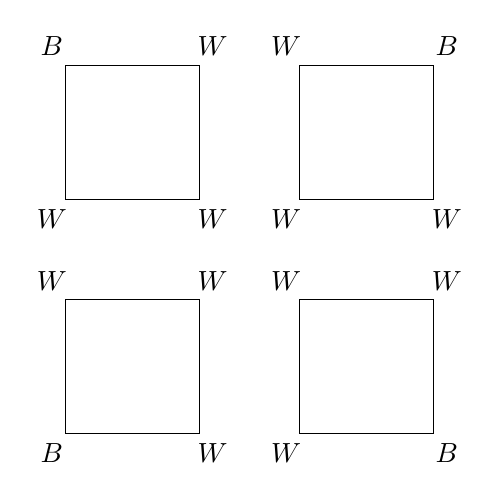
\begin{tikzpicture}[scale=0.85] %%Replaced figure with tikz figure - TWJ 6/28/2010

\draw (0,0) rectangle (2,2);
\node at (-0.2,0) [below] {$B$};
\node at (2.2,0) [below] {$W$};
\node at (-0.2,2) [above] {$W$};
\node at (2.2,2) [above] {$W$};

\draw (3.5,0) rectangle (5.5,2);
\node at (3.3,0) [below] {$W$};
\node at (5.7,0) [below] {$B$};
\node at (3.3,2) [above] {$W$};
\node at (5.7,2) [above] {$W$};

\draw (0,3.5) rectangle (2,5.5);
\node at (-0.2,3.5) [below] {$W$};
\node at (2.2,3.5) [below] {$W$};
\node at (-0.2,5.5) [above] {$B$};
\node at (2.2,5.5) [above] {$W$};


\draw (3.5,3.5) rectangle (5.5,5.5);
\node at (3.3,3.5) [below] {$W$};
\node at (5.7,3.5) [below] {$W$};
\node at (3.3,5.5) [above] {$W$};
\node at (5.7,5.5) [above] {$B$};

\end{tikzpicture}
\end{center}
\caption{Equivalent colorings of square}
\label{colorings}
\end{figure}
 
 
Burnside's Counting Theorem offers a method of computing the number of
distinguishable ways in which something can be done. In addition to
its geometric applications, the theorem has interesting applications
to areas in switching theory and chemistry. The proof of Burnside's
Counting Theorem depends on the following lemma.
 
 
\begin{lemma}\label{Gset_lemma}
Let $X$ be a $G$-set and suppose that $x \sim y$. Then $G_x$ is
isomorphic to $G_y$.  In particular, $|G_x| = |G_y|$. 
\end{lemma}
 
 
 %% Notation error pointed out by S. Engle corrected.
 %% TWJ 11/20/2011

\begin{proof}
Let $G$ act on $X$ by $(g,x) \mapsto g \cdot x$. Since $x \sim y$,
there exists a $g \in G$ such that $g \cdot x=y$. Let $a \in G_x$.
Since 
\[
gag^{-1} \cdot y = ga \cdot g^{-1}y = ga \cdot x = g \cdot
x = y,
\]
we can define a map $\phi: G_x \rightarrow G_y$ by $\phi(a) =
gag^{-1}$. The map $\phi$ is a homomorphism since 
\[
\phi(ab) = gabg^{-1} = gag^{-1} gbg^{-1} = \phi(a) \phi(b).
\]
Suppose that $\phi(a) = \phi(b)$. Then $gag^{-1}= gbg^{-1}$ or $a=b$;
hence, the map is injective.  To show that $\phi$ is onto, let $b$ be
in $G_y$; then $g^{-1}bg$ is in $G_x$ since
\[
g^{-1}bg \cdot x = g^{-1}b \cdot gx = g^{-1}b \cdot y = g^{-1} \cdot y
= x; 
\]
and $\phi(g^{-1}bg ) = b$.
\end{proof}
 
 
\begin{theorem}[Burnside]\index{Burnside's Counting Theorem}
Let $G$ be a  finite group acting on a set $X$ and let $k$ denote the
number of orbits of $X$. Then
\[
k = \frac{1}{|G|} \sum_{g \in G} |X_g|.
\]
\end{theorem}
 
 
\begin{proof}
We look at all the fixed points $x$ of all the elements in $g \in G$;
that is, we look at all $g$'s and all $x$'s such that $gx =x$.
If viewed in terms of fixed point sets, the number of all $g$'s fixing
$x$'s is 
\[
\sum_{g \in G} |X_g|.
\]
However, if viewed in terms of the stabilizer subgroups, this number
is 
\[
\sum_{x \in X} |G_x|;
\]
hence, $\sum_{g \in G} |X_g| = \sum_{x \in X} |G_x|$. By Lemma~\ref{Gset_lemma}, 
\[
\sum_{y \in {\mathcal O}_x} |G_y|  =  | {\mathcal O}_x| \cdot |G_x|.
\]
By Theorem~\ref{orbit_theorem} and Lagrange's Theorem, this expression is equal 
to $|G|$. Summing over all of the $k$ distinct orbits, we conclude that
\[
\sum_{g \in G} |X_g| = \sum_{x \in X} |G_x| = k \cdot |G|.
\]
\end{proof}
 
 
\begin{example}{Burnside_example}
Let $X = \{1, 2, 3, 4, 5 \}$ and suppose that $G$ is the permutation
group $G= \{(1), (1 3), (1 3)(2 5), (2 5) \}$. The orbits of $X$ are
$\{1, 3\}$, $\{2, 5\}$, and $\{4\}$. The fixed point sets are 
\begin{align*}
X_{(1)} & =  X \\
X_{(1 3)} & =  \{2, 4, 5 \} \\
X_{(1 3)(2 5)} & =  \{4\} \\
X_{(2 5)} & =  \{1, 3, 4 \} .
\end{align*}
Burnside's Theorem says that
\[
k = \frac{1}{|G|} \sum_{g \in G} |X_g| = \frac{1}{4}(5+
3+1+3) = 3.
\]
\end{example}
 
 
 
\subsection*{A Geometric Example}
 
 
 
Before we apply Burnside's Theorem to switching-theory problems, let
us examine the number of ways in which the vertices of a square can be
colored black or white. Notice that we can sometimes obtain equivalent
colorings by simply applying a rigid motion to the square. For
instance, as we have pointed out, if we color one of the vertices
black and the remaining three white, it does not matter which vertex
was colored black since a rotation will give an equivalent coloring.  
 
 
The  symmetry group of a square, $D_4$, is given by the following
permutations: 
\[
\begin{array}{cccc}
(1)    & (13)     & (24)     & (1432) \\
(1234) & (12)(34) & (14)(23) & (13)(24)
\end{array}
\]
The group $G$ acts on the set of vertices $\{ 1, 2, 3, 4\}$ in the
usual manner. We can describe the different colorings by mappings from
$X$ into $Y = \{ B, W \}$ where $B$ and $W$ represent the colors black
and white, respectively. Each map $f : X \rightarrow Y$ describes a
way to color the corners of the square. Every $\sigma \in D_4$ induces
a permutation $\widetilde{ \sigma }$ of the possible colorings given
by $\widetilde{\sigma}(f) = f \circ \sigma$ for $f : X \rightarrow Y$.
For example, suppose that $f$ is defined by 
\begin{align*}
f(1) & =  B \\
f(2) & =  W \\
f(3) & =  W \\
f(4) & =  W
\end{align*}
and $\sigma = (1 2)(3 4)$. Then $\widetilde{\sigma}(f) = f \circ
\sigma$ sends vertex 2 to $B$ and the remaining vertices to $W$. The
set of all such $\widetilde{\sigma}$ is a permutation group
$\widetilde{G}$ on the set of possible colorings. Let $\widetilde{X}$
denote the set of all possible colorings; that is, $\widetilde{X}$ is
the set of all possible maps from $X$ to $Y$.  Now we must compute the
number of $\widetilde{G}$-equivalence classes. 
\begin{enumerate}
 
\item
$\widetilde{X}_{(1)} = \widetilde{X}$ since the identity fixes every
possible coloring. $|\widetilde{X}| = 2^4 =~16$.
 
\item
$\widetilde{X}_{(1 2 3 4)}$ consists of all $f \in \widetilde{X}$ such
that $f$ is unchanged by the permutation $(1 23 4)$. In this case
$f(1) = f(2) = f(3) = f(4)$, so that all values of $f$ must be the 
same; that is, either $f(x)= B$ or $f(x)= W$ for every vertex $x$ of 
the square. So $|\widetilde{X}_{(1 2 3 4)}| = 2$.
 
\item 
$|\widetilde{X}_{(1 4 3 2)}| = 2$.
 
\item 
For $\widetilde{X}_{(1 3)(2 4)}$, $f(1) = f(3)$ and $f(2) =
f(4)$. Thus, $|\widetilde{X}_{(13)(24)}| = 2^2 = 4$.
 
\item 
$|\widetilde{X}_{(1 2)(3 4)}| = 4$.
 
\item 
$|\widetilde{X}_{(1 4)(2 3)}| = 4$.
 
\item 
For $\widetilde{X}_{(1  3 )}$, $f(1) = f(3)$ and the other corners can
be of any color; hence, $|\widetilde{X}_{(1 3)}| = 2^3 = 8$.
 
\item 
$|\widetilde{X}_{(2 4)}| = 8$.
 
\end{enumerate}
By Burnside's Theorem, we can conclude that there are exactly
\[
\frac{1}{8} ( 2^4 + 2^1 + 2^2 + 2^1  + 2^2 + 2^2 +2^3 + 2^3)
= 6
\]
ways to color the vertices of the square.
 
 
\begin{proposition}\label{actions:ActionFunctionProp}
Let $G$ be a permutation group of $X$ and $\widetilde{X}$ the set of
functions from $X$ to $Y$. Then there exists a permutation group 
$\widetilde{G}$ acting on $\widetilde{X}$, where $\widetilde{\sigma} 
\in \widetilde{G}$ is defined by $\widetilde{\sigma}(f) = f \circ 
\sigma$ for $\sigma \in G$ and $f \in \widetilde{X}$. Furthermore, 
if $n$ is the number of cycles in the cycle decomposition 
of $\sigma$, then $|\widetilde{X}_{\sigma}| = |Y|^n$. 
\end{proposition}
 
 
\begin{proof}
Let $\sigma \in G$ and $f \in  \widetilde{X}$. Clearly, $f \circ
\sigma$ is also in $\widetilde{X}$. Suppose that $g$ is another
function from $X$ to $Y$ such that $\widetilde{\sigma}(f) =
\widetilde{\sigma}(g)$. Then for each $x \in X$,
\[
f( \sigma(x ))
= \widetilde{\sigma}(f)(x)
= \widetilde{\sigma}(g)(x)
= g( \sigma(x )).
\]
Since $\sigma$ is a permutation of $X$, every element $x'$ in $X$ is
the image of some $x$ in $X$ under $\sigma$; hence, $f$ and $g$ agree
on all elements of $X$. Therefore, $f=g$ and $\widetilde{\sigma}$ is
injective.  The map $\sigma \mapsto \widetilde{\sigma}$ is onto, since
the two sets are the same size.
 
 
Suppose that $\sigma$ is a permutation of $X$ with cycle decomposition
$\sigma = \sigma_1 \sigma_2 \cdots \sigma_n$. Any $f$ in
${\widetilde{X}}_{\sigma}$ must have the same value on each cycle of
$\sigma$. Since there are $n$ cycles and $|Y|$ possible values for
each cycle, $|{\widetilde{X}}_{\sigma}| = |Y|^n$.
\mbox{\hspace{1in}}
\end{proof}
 
 
\begin{example}{burnside_X7}
Let $X = \{1, 2, \ldots, 7\}$ and suppose that $Y = \{ A, B, C \}$. If
$g$ is the permutation of $X$ given by $(1 3)(2 4 5) = (1 3)(2 4
5)(6)(7)$, then $n = 4$. Any $f \in {\mathcal F}_g$ must have the same
value on each cycle in $g$. There are $|Y|=3$ such choices for any
value, so $|{\mathcal F}_g|  = 3^4 = 81$.
\end{example}
 
 
 %Label problem fixed.  Suggested by L. Franklin.  TWJ 12/8/2011
\begin{example}{color_square}
Suppose that we wish to color the vertices of a square using four
different colors. By Proposition~\ref{actions:ActionFunctionProp}, we can immediately
decide that there are 
\[
\frac{1}{8} (4^4 + 4^1 + 4^2 + 4^1 + 4^2 + 4^ 2 + 4^3 + 4^3)
=55
\]
possible ways.
\end{example}
 
 
\begin{figure}[thb]


\begin{center}
\tikzpreface{actions_switching_function}
\begin{tikzpicture}[scale=1.25] %%Replaced figure with tikz figure - TWJ 6/28/2010

\draw (1,0) rectangle (2.7,2);
\node at (1.85,1)  {$f$};
\draw [->] (2.7,1) -- (3.2,1) node [right] {$f(x_1, x_2, \ldots, x_n)$};
\draw [->] (0.5,0.4) node [left] {$x_n$} -- (1,0.4);
\draw [->] (0.5,1.2) node [left] {$x_2$} -- (1,1.2);
\draw [->] (0.5,1.6) node [left] {$x_1$} -- (1,1.6);
\node at (0.5,0.85)  [left] {$\vdots$};

\end{tikzpicture}
\end{center}

\caption{A switching function of $n$ variables}
\label{nvariables}
\end{figure}
 
 
 
\subsection*{Switching Functions}
 
 
 
In switching theory we are concerned with the design of electronic
circuits with binary inputs and outputs. The simplest of these
circuits is a switching function that has $n$ inputs and a single output
(Figure~\ref{nvariables}). Large electronic circuits can often be 
constructed by combining smaller modules of this kind. The inherent
problem here is that even for a simple circuit a large number of
different switching functions can be constructed.  With only four
inputs and a single output, we can construct $65,536$ different
switching functions. However, we can often replace one switching
function with another merely by permuting the input leads to the
circuit (Figure~\ref{twovar}). 
 
 
\begin{figure}[htb]

\begin{center}
\tikzpreface{actions_switching_two_variables}
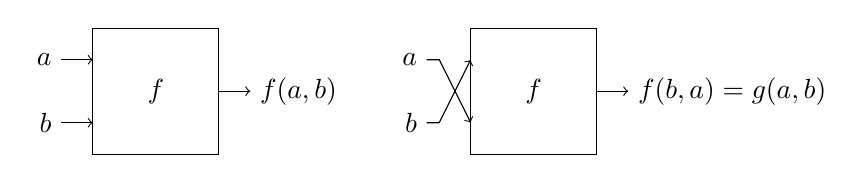
\begin{tikzpicture}[scale=0.8] %%Replaced figure with tikz figure - TWJ 6/28/2010

\draw (1,0) rectangle (3,2);
\node at (2,1)  {$f$};
\draw [->] (3,1) -- (3.5,1) node [right] {$f(a,b)$};
\draw [->] (0.5,1.5) node [left] {$a$} -- (1,1.5);
\draw [->] (0.5,0.5) node [left] {$b$} -- (1,0.5);

\draw (7,0) rectangle (9,2);
\node at (8,1)  {$f$};
\draw [->] (9,1) -- (9.5,1) node [right] {$f(b,a) = g(a,b)$};
\draw [->] (6.3,1.5) node [left] {$a$} -- (6.5,1.5) -- (7,0.5);
\draw [->] (6.3,0.5) node [left] {$b$} -- (6.5,0.5) -- (7,1.5);

\end{tikzpicture}
\end{center}

\caption{A switching function of two variables}
\label{twovar}
\end{figure}
 
 
We define a \boldemph{
switching}\index{Function!switching}\index{Switching function} or
\boldemph{Boolean
function}\index{Boolean function}\index{Function!Boolean} of $n$
variables to be a function from ${\mathbb Z}_2^n$ to ${\mathbb Z}_2$. Since 
any switching function can have two possible values for each binary
$n$-tuple and there are $2^n$ binary $n$-tuples, $2^{2^n}$ switching
functions are possible for $n$ variables. In general, allowing
permutations of the inputs greatly reduces the number of different
kinds of modules that are needed to build a large circuit.
 
 
The possible switching functions  with two input variables $a$ and
$b$ are listed in Table~\ref{switching_2variable}. Two switching functions $f$ and $g$
are equivalent if $g$ can be obtained from $f$ by a permutation of the
input variables. For example, $g(a, b, c) = f(b, c, a)$. In this 
case $g \sim f$ via the permutation $(acb)$. In the case of switching
functions of two variables, the permutation $(ab)$ reduces 16
possible switching functions to 12 equivalent functions since
\begin{align*}
f_2 & \sim  f_4 \\
f_3 & \sim  f_5 \\
f_{10} & \sim  f_{12} \\
f_{11} & \sim  f_{13}.
\end{align*}
 
 
\begin{table}[htb]
\caption{Switching functions in two variables}{\small
\medskip
\begin{center}
\begin{tabular}{|cc|cccccccc|}
\hline
\multicolumn{2}{|c|}{Inputs}
 & \multicolumn{8}{|c|}{Outputs}    \\
\hline
         &     & $f_0$ & $f_1$ & $f_2$ & $f_3$ & $f_4$ &
$f_5$ & $f_6$ & $f_7$  \\ \hline
0 & 0   & 0 & 0 & 0 & 0 & 0 & 0 & 0 & 0 \\
0 & 1   & 0 & 0 & 0 & 0 & 1 & 1 & 1 & 1 \\
1 & 0   & 0 & 0 & 1 & 1 & 0 & 0 & 1 & 1 \\
1 & 1   & 0 & 1 & 0 & 1 & 0 & 1 & 0 & 1 \\ \hline\hline
\multicolumn{2}{|c|}{Inputs}
 & \multicolumn{8}{|c|}{Outputs}    \\
\hline
         &     & $f_8$ & $f_9$ & $f_{10}$ & $f_{11}$
& $f_{12}$ & $f_{13}$ & $f_{14}$ & $f_{15}$ \\ \hline
0 & 0   & 1 & 1 & 1 & 1 & 1 & 1 & 1 & 1 \\
0 & 1   & 0 & 0 & 0 & 0 & 1 & 1 & 1 & 1 \\
1 & 0   & 0 & 0 & 1 & 1 & 0 & 0 & 1 & 1 \\
1 & 1   & 0 & 1 & 0 & 1 & 0 & 1 & 0 & 1 \\ \hline
\end{tabular}
\end{center}\label{switching_2variable}
}
\end{table}
 
 
For three input variables there are $2^{2^3}=256$ possible switching
functions; in the case of four variables there are $2^{2^4} =
\mbox{65,536}$. The number of equivalence classes is too large to reasonably
calculate directly. It is necessary to employ  Burnside's Theorem.
 
 
Consider a  switching function with three possible inputs, $a$, $b$,
and $c$. As we have mentioned, two switching functions $f$ and $g$ are
equivalent if a permutation of the input variables of $f$ gives $g$.
It is important to notice that a permutation of the switching
functions is not simply a permutation of the input values $\{a, b,
c\}$. A switching function is a set of output values for the inputs
$a$, $b$, and $c$, so when we consider equivalent switching functions, we
are permuting $2^3$ possible outputs, not just three input values. For
example, each binary triple $(a, b, c)$ has a specific output
associated with it. The  permutation $(acb)$ changes outputs as follows: 
\begin{align*}
(0, 0, 0) & \mapsto  (0, 0, 0) \\
(0, 0, 1) & \mapsto  (0, 1, 0) \\
(0, 1, 0) & \mapsto  (1, 0, 0) \\
& \vdots  \\
(1, 1, 0) & \mapsto  (1, 0, 1) \\
(1, 1, 1) & \mapsto  (1, 1, 1).
\end{align*}

Let $X$ be the set of output values for a switching function in $n$
variables. Then $|X|=2^n$. We can enumerate these values as follows: 
\begin{align*}
(0, \ldots, 0, 1) & \mapsto  0 \\
(0, \ldots, 1, 0) & \mapsto  1 \\
(0, \ldots, 1, 1) & \mapsto  2 \\
& \vdots  \\
(1, \ldots, 1, 1) & \mapsto  2^n-1.
\end{align*}
Now let us consider a circuit with four input variables and a single
output. Suppose that we can permute the leads  of any circuit
according to the following permutation group: 
\begin{gather*}
(a)    \quad (ac)     \quad (bd)     \quad (adcb) \\
(abcd) \quad (ab)(cd) \quad (ad)(bc) \quad (ac)(bd).
\end{gather*}
The permutations of the four possible input variables induce the
permutations of the output values in Table~\ref{switching_permute}. 
 
 

 
 
Hence, there are
\[
\frac{1}{8} (2^{16} + 2 \cdot 2^{12} + 2 \cdot 2^6 + 3 \cdot
2^{10}) = 9616
\]
possible switching functions of four variables under this group of
permutations. This number will be even smaller if we consider the full
symmetric group on four letters. 
 
 
 \begin{table}[htb]
\caption{Permutations of switching functions in four variables}{\small 
\medskip
\begin{center}
\begin{tabular}{|l|l|l|}
\hline
Group       &                                 &  Number  \\
Permutation &  Switching Function Permutation &  of Cycles  \\
\hline
$(a)$        & $(0)$ & 16 \\
$(a c)$      & $(2,8)(3,9)(6,12)(7,13)$ & 12 \\
$(b d)$      & $(1,4)(3,6)(9,12)(11,14)$ & 12 \\
$(a d c b)$  & $(1,2,4,8)(3,6.12,9)(5,10)(7,14,13,11)$ & 6\\
$(a b c d)$  & $(1,8,4,2)(3,9,12,6)(5,10)(7,11,13,14)$ & 6\\
$(a b)(c d)$ & $(1,2)(4,8)(5,10)(6,9)(7,11)(13,14)$ & 10\\
$(a d)(b c)$ & $(1,8)(2,4)(3,12)(5,10)(7,14)(11,13)$ & 10\\
$(a c)(b d)$ & $(1,4)(2,8)(3,12)(6,9)(7,13)(11,14)$ & 10 \\
\hline
\end{tabular}
\end{center}\label{switching_permute}
}
\end{table}
\histhead
 
 
 
\noindent{\small \histf
William Burnside\index{Burnside, William} was born in London in 1852.
He attended Cambridge University from 1871 to 1875 and won the Smith's
Prize in his last year.  After his graduation he lectured at
Cambridge.  He was made a member of the Royal Society in 1893.
Burnside wrote approximately 150 papers on topics in applied
mathematics, differential geometry, and probability, but his most
famous contributions were in group theory.  Several of Burnside's
conjectures have stimulated research to this day.  One such conjecture
was that every group of odd order is solvable; that is, for a group
$G$ of odd order, there exists a sequence of subgroups 
\[
G = H_n \supset H_{n-1} \supset \cdots \supset H_1 \supset
H_0 = \{ e \}
\]
such that $H_i$ is normal in $H_{i+1}$ and $H_{i+1} / H_i$ is abelian.
This conjecture was finally proven by W. Feit\index{Feit, W.}
and J. Thompson\index{Thompson, J.} in 1963. 
Burnside's  \textit{The Theory of Groups of Finite Order},
published in 1897, was one of the first books to treat groups in a
modern context as 
opposed to permutation groups. The second edition, published in 1911,
is still a classic. 
\histbox
}
 
 
 
\markright{EXERCISES}
\section*{Exercises}
\exrule
 
 
 
 
{\small
\begin{enumerate}
 
%***************Calculations************************

% 2010/05/10 R Beezer: made it clearer what the G-equivalence classes are
\item
Examples~\ref{example:actions:GL2_action}--\ref{example:actions:left_coset_action}  in the first section each describe an action of a group $G$ on a set $X$, which will give rise to the equivalence relation defined by $G$-equivalence.  For each example, compute the equivalence classes of the equivalence relation,  the \boldemph{$G$-equivalence classes}\index{$G$-equivalence classes}.
 
 
\item \label{actions:computation:exercise}
Compute all $X_g$ and all $G_x$ for each of the following permutation
groups. 
\begin{enumerate}
 
 \item
$X= \{1, 2, 3\}$, \\
$G=S_3=\{(1), (12), (13), (23), (123), (132)  \}$
 
 \item
$X = \{1, 2, 3, 4, 5, 6\}$, \\
$G = \{(1), (12), (345), (354), (12)(345), (12)(354)  \}$
 
\end{enumerate}
 
 
\item
Compute the $G$-equivalence classes of $X$ for each of the $G$-sets in
Exercise~\ref{actions:computation:exercise}. For each $x \in X$ verify that $|G|=|{\mathcal O}_x| \cdot
|G_x|$.  
 
 
\item
Let $G$ be the additive group of real numbers. Let the action of
$\theta \in G$ on the real plane ${\mathbb R}^2$ be given by rotating the
plane counterclockwise about the origin through $\theta$ radians. Let
$P$ be a point on the plane other than the origin.
\begin{enumerate}
 
 \item
Show that ${\mathbb R}^2$ is a $G$-set.
 
 \item
Describe geometrically the orbit containing $P$.
 
 \item
Find the group $G_P$.
 
\end{enumerate}
 
 
\item
Let $G =  A_4$ and suppose that $G$ acts on itself by conjugation;
that is, $(g,h)~\mapsto~ghg^{-1}$. 
\begin{enumerate}
 
 \item
Determine the conjugacy classes (orbits) of each element of $G$.
 
 \item
Determine all of the isotropy subgroups for each element of $G$.
 
\end{enumerate}
 
 
\item
Find the conjugacy classes and the class equation for each of the
following groups. 
\begin{multicols}{4}
\begin{enumerate}

\item
$S_4$

\item
$D_5$

\item
${\mathbb Z}_9$

\item
$Q_8$


\end{enumerate}
\end{multicols}
 

 
 
\item  %%%%%%%%%%%%%%%%
Write the class equation for $S_5$ and for $A_5$.
 
 
\item
If a square remains fixed in the plane, how many different ways can
the corners of the square be colored if three colors are used?
 
 
\item
How many ways can the vertices of an equilateral triangle be colored
using three different colors? 
 
 
\item
Find the number of ways a six-sided die can be constructed if each
side is  marked differently with $1, \ldots, 6$ 
dots.
 
\item
Up to a rotation, how many ways can the faces of a cube be colored
with three different colors? 
 
 
 
\item
Consider 12 straight wires of equal lengths with their ends soldered
together to form the edges of a cube. Either silver or copper wire can be
used for each edge.  How many different ways can the cube be
constructed? 
 
 
 
\item
Suppose that we color each of the eight corners of a cube. Using three
different colors, how many ways can the corners be colored up to a
rotation of the cube? 
 
 
\item
Each of the faces of a regular tetrahedron can be painted either red
or white.  Up to a rotation, how many different ways can the
tetrahedron be painted? 
 
 
\item
Suppose that the vertices of a regular hexagon are to be colored either
red or white.  How many ways can this be done up to a symmetry  of the
hexagon? 
 
 
\item
A molecule of benzene is made up of six carbon atoms and six hydrogen
atoms, linked together in a hexagonal shape as in Figure~\ref{benzene}.
\begin{enumerate}
 
 \item
How many different compounds can be formed by replacing one or more of
the hydrogen atoms with a chlorine atom? 
 
 \item
Find the number of different chemical compounds that can be formed by
replacing three of the six hydrogen atoms in a benzene ring with a
$CH_3$ radical.
 
\end{enumerate}
 
 
\begin{figure}[ht]
\begin{center}
\tikzpreface{actions_benzene}
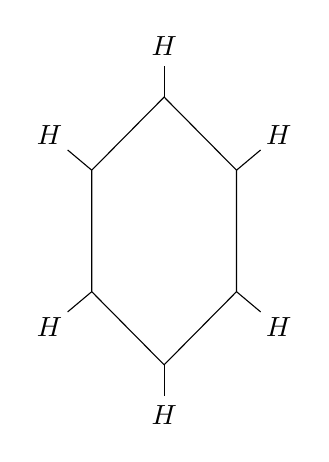
\begin{tikzpicture}[scale=1.0] %%Replaced figure with tikz figure - TWJ 6/28/2010

\draw (40:1.2) -- (90:1.7) -- (140:1.2) -- (220:1.2) -- (270:1.7) -- (320:1.2) -- cycle;
\draw (90:1.7) -- (90:2.1) node [above] {$H$};
\draw (270:1.7) -- (270:2.1) node [below] {$H$};
\draw (40:1.2) -- (40:1.6);
\node at (40:1.9) {$H$};
\draw (140:1.2) -- (140:1.6);
\node at (140:1.9) {$H$};
\draw (220:1.2) -- (220:1.6);
\node at (220:1.9) {$H$};
\draw (320:1.2) -- (320:1.6);
\node at (320:1.9) {$H$};

\end{tikzpicture}
\end{center}
\caption{A benzene ring}
\label{benzene}
\end{figure}
 
 
\item
How many equivalence classes of switching functions are there if the
input variables $x_1$, $x_2$, and $x_3$ can be permuted by any
permutation in $S_3$? What if the input variables $x_1$, $x_2$, $x_3$,
and $x_4$ can be permuted by any permutation in $S_4$?
 
 
\item
How many equivalence classes of switching functions are there if the
input variables $x_1$, $x_2$, $x_3$, and $x_4$ can be permuted by any
permutation in the subgroup of $S_4$ generated by the permutation
$(x_1 x_2 x_3 x_4)$?  
 
 
\item
A striped necktie has 12 bands of color. Each band can be colored
by one of four possible colors.  How many possible different-colored
neckties are there? 
 
 
%***************Theory******************************
 
 
\item
A group acts \boldemph{faithfully} on a $G$-set $X$ if the identity is the
only element of $G$ that leaves every element of $X$ fixed. Show that
$G$ acts faithfully  on $X$ if and only if no two distinct elements of
$G$ have the same action on each element of $X$.
 
 
\item
Let $p$ be prime. Show that the number of different abelian groups of
order $p^n$ (up to isomorphism)  is the same as the number of
conjugacy classes in $S_n$. 
 
 
\item
Let $a \in G$. Show that for any $g \in G$, $gC(a) g^{-1} =
C(gag^{-1})$. 
 
 
\item
Let $|G| = p^n$ and suppose that $|Z(G)| = p^{n-1}$ for  $p$ prime.
Prove that $G$ is abelian. 
 
 
\item
Let $G$ be a group with order $p^n$ where $p$ is prime and $X$ a
finite $G$-set.  If $X_G = \{ x \in X : gx = x \text{ for all }g \in
G \}$ is the set of elements in $X$ fixed by the group action, then
prove that $|X| \equiv |X_G| \pmod{ p}$.

\item
If $G$ is a group of order $p^n$, where $p$ is prime and $n \geq 2$, show that $G$ must have a proper subgroup of order $p$.  If $n \geq 3$, is it true that $G$ will have a proper subgroup of order $p^2$?
%Moved problem from cosets.tex TWJ 12/19/2011
 
 
\end{enumerate}
}
 
 
 
\subsection*{Programming Exercise}
 
 
 
{\small
Write a program to compute the number of conjugacy classes in $S_n$.
What is the largest $n$ for which your program will work?
}
 
 
 
\subsection*{References and Suggested Reading} %%TWJ 6/28/2010 - References checked.
 
 
 
{\small
\begin{itemize}
 
\item[\textbf{[1]}]
De Bruijin, N. G. ``P\'{o}lya's Theory of Counting,'' in {\it
Applied Combinatorial Mathematics}, Beckenbach, E. F., ed.
Wiley, New York, 1964.
 
\item[\textbf{[2]}]
Eidswick, J. A. ``Cubelike Puzzles---What Are They and How
Do You Solve Them?'' \textit{American Mathematical
Monthly} \textbf{93} (1986), 157--76.
 
\item[\textbf{[3]}]
Harary, F., Palmer, E. M., and Robinson, R. W. ``P\'{o}lya's
Contributions to Chemical Enumeration,'' in \textit{Chemical
Applications of Graph Theory}, Balaban, A. T., ed. Academic
Press, London, 1976.
 
\item[\textbf{[4]}] %%TWJ 6/28/2010 - This is out of print
G{\aa}ding, L. and Tambour, T. \textit{Algebra for Computer
Science}. Springer-Verlag, New York, 1988.
 
\item[\textbf{[5]}] %%TWJ 6/28/2010 - This is out of print
Laufer, H. B. \textit{Discrete Mathematics and Applied Modern
Algebra}. PWS-Kent, Boston, 1984.
 
 
\item[\textbf{[6]}] %%TWJ 6/28/2010 - This is out of print
P\'{o}lya, G. and Read, R. C. \textit{Combinatorial Enumeration
of Groups, Graphs, and Chemical Compounds}. Springer-Verlag,
New York, 1985.
 
\item[\textbf{[7]}]
Shapiro, L. W. ``Finite Groups Acting on Sets with
Applications,'' \textit{Mathematics Magazine}, May--June 1973,
136--47.
 
\end{itemize}
}
 
\sagesection
 
  %Group Actions
%%%%(c)
%%%%(c)  This file is a portion of the source for the textbook
%%%%(c)
%%%%(c)    Abstract Algebra: Theory and Applications
%%%%(c)    by Thomas W. Judson
%%%%(c)
%%%%(c)    Sage Material
%%%%(c)    Copyright 2011 by Robert A. Beezer
%%%%(c)
%%%%(c)  See the file COPYING.txt for copying conditions
%%%%(c)
%%%%(c)
\begin{sageverbatim}\end{sageverbatim}
%
\sageexercise{1}%
This exercise verifies Theorem~\extref{sylow:commutator_subgroup_theorem}{15.9}{quotient by commutator is abelian}.  The commutator subgroup is computed with the permutation group method \verb?.commutator()?.  For the dihedral group of order 40, $D_{20}$ (\verb?DihedralGroup(20)? in Sage), compute the commutator subgroup and form the quotient with the dihedral group.  Then verify that this quotient is abelian.  Can you identify the quotient group exactly (in other words, up to isomorphism)?
\begin{sageverbatim}\end{sageverbatim}
%
\sageexercise{2}%
For each possible prime, find all of the distinct Sylow $p$-subgroups of the alternating group $A_5$.  Confirm that your results are consistent with the Third Sylow Theorem for each prime.  We know that $A_5$ is a simple group.  Explain how this would explain or predict some aspects of your answers.\par
%
Count the number of distinct elements contained in the union of all the Sylow subgroups you just found.  What is interesting about this count?
\begin{sageverbatim}\end{sageverbatim}
%
\sageexercise{3}%
For each possible prime, find all of the distinct Sylow $p$-subgroups of the dihedral group $D_{36}$ (symmetries of a $36$-gon) for each possible prime.  Confirm that your results are consistent with the Third Sylow Theorem for each prime.  It can be proved that {\em any group} with order $72$ is not a simple group, using techniques such as those used in the later examples in this chapter.  Explain how this result would explain or predict some aspects of your answers.\begin{sageverbatim}\end{sageverbatim}
%
\sageexercise{4}%
This exercise verifies Lemma~\extref{distinct_conj_lemma}{15.5}{number of conjugacy classes}.  Let $G$ be the dihedral group of order $36$, $D_{18}$.  Let $H$ be the one Sylow $3$-subgroup.  Let $K$ be the subgroup of order $6$ generated by the two permutations \verb?a? and \verb?b? given below.  First, form a list of the distinct conjugates of $K$ by the elements of $H$, and determine the number of subgroups in this list.  Compare this with the index given in the statement of the lemma, employing a single (long) statement making use of the \verb?.order()?, \verb?.normalizer()? and \verb?.intersection()? methods.\par
%
\begin{sageexample}
sage: G = DihedralGroup(18)
sage: a = G("(1,7,13)(2,8,14)(3,9,15)(4,10,16)(5,11,17)(6,12,18)")
sage: b = G("(1,5)(2,4)(6,18)(7,17)(8,16)(9,15)(10,14)(11,13)")
\end{sageexample}
%
\begin{sageverbatim}\end{sageverbatim}
%
\sageexercise{5}%
Example~\extref{example:sylow:G48}{9}{example on order 48 subgroup} shows that every group of order $48$ has a normal subgroup.  The dicyclic groups are an infinite family of non-abelian groups with order $4n$, which includes the quaternions when $n=2$.  So the permutation group \verb?DiCyclicGroup(12)? has order 48.  Use Sage to follow the logic of the proof in Example~\extref{example:sylow:G48}{9}{example on order 48 subgroup} and construct a normal subgroup in this group.  (In other words, do not just ask for a list of the normal subgroups, but trace through the implications in the example to arrive at the normal subgroup, and check your answer.)
\begin{sageverbatim}\end{sageverbatim}
%
    %Sylow Theorems
%%%%(c)
%%%%(c)  This file is a portion of the source for the textbook
%%%%(c)
%%%%(c)    Abstract Algebra: Theory and Applications
%%%%(c)    by Thomas W. Judson
%%%%(c)
%%%%(c)    Sage Material
%%%%(c)    Copyright 2011 by Robert A. Beezer
%%%%(c)
%%%%(c)  See the file COPYING.txt for copying conditions
%%%%(c)
%%%%(c)
Rings are very important in your study of abstract algebra, and similarly, they are very important in the design and use of Sage.  There is a lot of material in this chapter, and there are many corresponding commands in Sage.
%
\sagesubsection{Creating Rings}
%
Here is a list of various rings, domains and fields you can construct simply.\par
%
1. \verb?Integers()?, \verb?ZZ?: the integral domain of positive and negative integers, ${\mathbb Z}$.\par
%
2.  \verb?Integers(n)?: the integers mod $n$, ${\mathbb Z_n}$.  A field when $n$ is prime, but just a ring for composite $n$.\par
%
3.  \verb?QQ?: the field of rational numbers, ${\mathbb Q}$.\par
%
4.  \verb?RR?, \verb?CC?: the field of real numbers and the field of complex numbers, ${\mathbb R}$, ${\mathbb C}$.  It is impossible to create \emph{every} real number inside a computer, so technically these sets do not behave as fields, but only give a good imitiation of the real thing.  We say they are ``inexact'' rings to make this point.\par
%
5.  \verb?QuadraticField(n)?:  the field formed by combining the rationals with a solution to the polynomial equation $x^2-n=0$.  The notation in the text is ${\mathbb Q}[\sqrt{n}]$.  A functional equivalent can be made with the syntax \verb?QQ[sqrt(n)]?.  Note that \verb?n? can be negative.\par
%
6.  \verb?CyclotomicField(n)?: the field formed by combining the rationals with the solutions to the polynomial equation $x^n-1=0$.\par
%
7.  \verb?QQbar?: the field formed by combining the rationals with the solutions to \emph{every} polynomial equation with integer coefficients.  This is known as a the field of algebraic numbers, denoted as $\overline{{\mathbb Q}}$.\par
%
8.  \verb?FiniteField(p)?: For a prime $p$, the field of integers ${\mathbb Z_p}$.\par
%
If you print a description of some of the above rings, you will sometimes see a new symbol introduced.  Consider the following example:
%
\begin{sageexample}
sage: F = QuadraticField(7)
sage: F
Number Field in a with defining polynomial x^2 - 7
sage: root = F.gen(0)
sage: root^2
7
sage: root
a
sage: (2*root)^3
56*a
\end{sageexample}
%
Here \verb?Number Field? describes an object generally formed by combining the rationals with another number (here $\sqrt{7}$).  ``a'' is a new symbol which behaves as a root of the polynomial $x^2-7$.  We do not say which root, $\sqrt{7}$ or $-\sqrt{7}$, and as we understand the theory better we will see that this does not really matter.\par
%
We can obtain this root as a generator of the number field, and then manipulate it.  First squaring \verb?root? yields 7.  Notice that \verb?root? prints as \verb?a?.  Notice, too, that computations with \verb?root? behave as if it was \emph{either} root of $x^2-7$, and results print using \verb?a?.\par
%
This can get a bit confusing, inputing computations with \verb?root? and getting output in terms of \verb?a?.  Fortunately, there is a better way.  Consider the following example:
%
\begin{sageexample}
sage: F.<b> = QuadraticField(7)
sage: F
Number Field in b with defining polynomial x^2 - 7
sage: b^2
7
sage: (2*b)^3
56*b
\end{sageexample}
%
With the syntax \verb?F.<b>? we can create the field \verb?F? along with specifying a generator \verb?b? using a name of our choosing.  Then computations can use \verb?b? in both input and output as a root of $x^2-7$.\par
%
Here are three new rings that are best created using this new syntax.\par
%
1. \verb?F.<a> = FiniteField(p^n)?: We will later have a theorem that tells us that finite fields only exist with orders equal to to a power of a prime.  When the power is larger than 1, then we need a gnerator, here given as \verb?a?.\par
%
2. \verb?P.<x>=R[]?: the ring of all polynomials in the variable \verb?x?, with coefficients from the ring \verb?R?.  Notice that \verb?R? can be \emph{any} ring, so this is a very general construction that uses one ring to form another.  See an example below.\par
%
3. \verb?Q.<r,s,t> = QuaternionAlgebra(n, m)?: the rationals combined with indeterminates \verb?r?, \verb?s? and \verb?t? such that $r^2=n$, $s^2=m$ and $t = rs = -sr$.  This is a generalization of the quaternions described in this chapter, though over the rationals rather than the reals, so it is an exact ring.  Notice that this is one of the few noncommutative rings in Sage.  The ``usual'' quaternions would be constructed with \verb?Q.<I,J,K> = QuaternionAlgebra(-1, -1)?.  (Notice that using \verb?I? here is not a good choice, because it will then clobber the symbol \verb?I? used for complex numbers.)
\par
%
Syntax specifying names for generators can be used for many of the above rings as well, such as demonstrated above for quadratic fields and below for cyclotomic fields.
%
\begin{sageexample}
sage: C.<t> = CyclotomicField(8)
sage: C.random_element()  # random
-2/11*t^2 + t - 1
\end{sageexample}
%
\sagesubsection{Properties of Rings}
%
The examples below demonstrate how to query certain properties of rings.  If you are playing along, be sure to execute the first compute cell to define the various rings involved in the examples.
%
\begin{sageexample}
sage: Z7 = Integers(7)
sage: Z9 = Integers(9)
sage: Q = QuadraticField(-11)
sage: F.<a> = FiniteField(3^2)
sage: P.<x> = Z7[]
sage: S.<f,g,h> = QuaternionAlgebra(-7, 3)
\end{sageexample}
%
Exact versus inexact.
%
\begin{sageexample}
sage: QQ.is_exact()
True
sage: RR.is_exact()
False
\end{sageexample}
%
Finite versus infinite.
%
\begin{sageexample}
sage: Z7.is_finite()
True
sage: P.is_finite()
False
\end{sageexample}
%
Integral domain?
%
\begin{sageexample}
sage: Z7.is_integral_domain()
True
sage: Z9.is_integral_domain()
False
\end{sageexample}
%
Field?
%
\begin{sageexample}
sage: Z9.is_field()
False
sage: F.is_field()
True
sage: Q.is_field()
True
\end{sageexample}
%
Commutative?
%
\begin{sageexample}
sage: Q.is_commutative()
True
sage: S.is_commutative()
False
\end{sageexample}
%
Characteristic.
%
\begin{sageexample}
sage: Z7.characteristic()
7
sage: Z9.characteristic()
9
sage: Q.characteristic()
0
sage: F.characteristic()
3
sage: P.characteristic()
7
sage: S.characteristic()
0
\end{sageexample}
%
Additive and multiplicative identities \emph{print} like you would expect, but notice that while they may \emph{print} identically, they could be \emph{different} because of the ring they are in.
%
\begin{sageexample}
sage: b = Z9.zero(); b
0
sage: b.parent()
Ring of integers modulo 9
sage: c = Q.zero(); c
0
sage: c.parent()
Number Field in a with defining polynomial x^2 + 11
sage: b == c
False
sage: d = Z9.one(); d
1
sage: d.parent()
Ring of integers modulo 9
sage: e = Q.one(); e
1
sage: e.parent()
Number Field in a with defining polynomial x^2 + 11
sage: d == e
False
\end{sageexample}
%
There is some support for subrings.  For example, \verb?Q? and \verb?S? are extensions of the rationals, while \verb?F? is totally distinct from the rationals.
%
\begin{sageexample}
sage: QQ.is_subring(Q)
True
sage: QQ.is_subring(S)
True
sage: QQ.is_subring(F)
False
\end{sageexample}
%
Not every element of a ring may have a multiplicative inverse, in other words, not every element has to be a unit (unless the ring is a field).  It would now be good practice to check if an element is a unit before you try computing its inverse.
%
\begin{sageexample}
sage: three = Z9(3)
sage: three.is_unit()
False
sage: three*three
0
sage: four = Z9(4)
sage: four.is_unit()
True
sage: g = four^-1; g
7
sage: four*g
1
\end{sageexample}
%
\sagesubsection{Quotient Structure}
%
Ideals are the normal subgroups of rings and allow us to build ``quotients'' --- basically new rings defined on equivalence classes of elements of the original ring.  Sage support for ideals is variable.  When they can be created, there is not always a lot you can do with them.  But they work well in certain very important cases.
%
The integers, ${\mathbb Z}$, have ideals that are just multiples of a single integer.  We can create them with the \verb?.ideal()? method or just by wrting a scalar multiple of \verb?ZZ?.  And then the quotient is isomorphic to a well-understood ring.  (Notice that \verb?I? is a bad name for an ideal if we want to work with complex numbers later.)
%
\begin{sageexample}
sage: I1 = ZZ.ideal(4)
sage: I2 = 4*ZZ
sage: I3 = (-4)*ZZ
sage: I1 == I2
True
sage: I2 == I3
True
sage: Q = ZZ.quotient(I1); Q
Ring of integers modulo 4
sage: Q == Integers(4)
True
\end{sageexample}
%
We might normally be more careful about the last statement.  The quotient is a set of equivalence classes, each infinite, and certainly not a single integer.  But the quotient is \emph{isomorphic} to ${\mathbb Z}_4$, so Sage just makes this identification.\par
%
\begin{sageexample}
sage: Z7 = Integers(7)
sage: P.<y> = Z7[]
sage: M = P.ideal(y^2+4)
sage: Q = P.quotient(M)
sage: Q
Univariate Quotient Polynomial Ring in ybar over
Ring of integers modulo 7 with modulus y^2 + 4
sage: Q.random_element() # random
2*ybar + 6
sage: Q.order()
49
sage: Q.is_field()
True
\end{sageexample}
%
Notice that the construction of the quotient ring has created a new generator, converting \verb?y? ($y$) to \verb?ybar? ($\overline{y}$).  We can override this as before with the syntax demonstrated below.
%
\begin{sageexample}
sage: Q.<t> = P.quotient(M); Q
Univariate Quotient Polynomial Ring in t over
Ring of integers modulo 7 with modulus y^2 + 4
sage: Q.random_element() # random
4*t + 6
\end{sageexample}
%
So from a quotient of an infinite ring and an ideal (which is also a ring), we create a field, which is finite.  Understanding this construction will be an important theme in the next few chapters.  To see how remarkable it is, consider what happens with just one little change.
%
\begin{sageexample}
sage: Z7 = Integers(7)
sage: P.<y> = Z7[]
sage: M = P.ideal(y^2+3)
sage: Q.<t> = P.quotient(M)
sage: Q
Univariate Quotient Polynomial Ring in t over
Ring of integers modulo 7 with modulus y^2 + 3
sage: Q.random_element() #random
3*t + 1
sage: Q.order()
49
sage: Q.is_field()
False
\end{sageexample}
%
There are a few methods available which will give us properties of ideals.  In particular, we can check for prime and maximal ideals in rings of polynomials.  Examine the results above and below in the context of Theorem~\ref{theorem:maximalfield}.
%
\begin{sageexample}
sage: Z7 = Integers(7)
sage: P.<y> = Z7[]
sage: M = P.ideal(y^2+4)
sage: N = P.ideal(y^2+3)
sage: M.is_maximal()
True
sage: N.is_maximal()
False
\end{sageexample}
%
The fact that \verb?M? is a prime ideal is verification of Corollary~\ref{rings:max_ideal_corollary}.
%
\begin{sageexample}
sage: M.is_prime()
True
sage: N.is_prime()
False
\end{sageexample}
%
\sagesubsection{Ring Homomorphisms}
%
When Sage is presented with \verb?3 + 4/3?, how does it know that 3 is meant to be an integer? And then to add it to a rational, how does it know that we really want to view the computation as 3/1 + 4/3?  This is really easy for you and me, but devilishly hard for a program, and you can imagine it getting ever more complicated with the many possible rings in Sage, subrings, matrices, etc.  Part of the answer is that Sage uses ring homomorphisms to ``translate'' objects (numbers) between rings.\par
%
We will give an example below, but not pursue the topic much further.  For the curious, reading the Sage documentation and experimenting would be a good exercise.
%
\begin{sageexample}
sage: H = Hom(ZZ, QQ)
sage: phi = H([1])
sage: phi
Ring morphism:
  From: Integer Ring
  To:   Rational Field
  Defn: 1 |--> 1
sage: phi.parent()
Set of Homomorphisms from Integer Ring to Rational Field
sage: a = 3; a
3
sage: a.parent()
Integer Ring
sage: b = phi(3); b
3
sage: b.parent()
Rational Field
\end{sageexample}
%
So \verb?phi? is a homomorphism (``morphism'') that converts integers (the domain is \verb?ZZ?) into rationals (the codomain is \verb?QQ?), whose parent is a set of homomorphisms that Sage calls a ``homset.''  Even though \verb?a? and \verb?b? both print as \verb?3?, which is indistinguishable to our eyes, the parents of \verb?a? and \verb?b? are different.  Yet the numerical value of the two objects has not changed.
%




    %Introduction to Rings
%%%%(c)
%%%%(c)  This file is a portion of the source for the textbook
%%%%(c)
%%%%(c)    Abstract Algebra: Theory and Applications
%%%%(c)    by Thomas W. Judson
%%%%(c)
%%%%(c)    Sage Material
%%%%(c)    Copyright 2011 by Robert A. Beezer
%%%%(c)
%%%%(c)  See the file COPYING.txt for copying conditions
%%%%(c)
%%%%(c)
Polynomial rings are very important for computational approaches to algebra, and so Sage makes it very easy to compute with polynomials, over rings, or over fields.  And it is trivial to check if a polynomial is irreducible.     %Polynomial Rings
%%%%(c)
%%%%(c)  This file is a portion of the source for the textbook
%%%%(c)
%%%%(c)    Abstract Algebra: Theory and Applications
%%%%(c)    by Thomas W. Judson
%%%%(c)
%%%%(c)    Sage Material
%%%%(c)    Copyright 2011 by Robert A. Beezer
%%%%(c)
%%%%(c)  See the file COPYING.txt for copying conditions
%%%%(c)
%%%%(c)
We have already seen some integral domains and unique factorizations in the previous two chapters.  In addition to what we have already seen, Sage has support for some of the topics from this section, but the coverage is limited.  Some functions will work for some rings and not others, while some functions are not yet part of Sage.  So we will give some examples, but this is far from comprehensive.
%
\sagesubsection{Field of Fractions}
%
Sage is frequently able to construct a field of fractions, or identify a certain field as the field of fractions.  For example, the ring of integers and the field of rational numbers are both implemented in Sage, and the integers ``know'' that the rationals is it's field of fractions.
%
\begin{sageexample}
sage: Q = ZZ.fraction_field(); Q
Rational Field
sage: Q == QQ
True
\end{sageexample}
%
In other cases Sage will construct a fraction field, in the spirit of Lemma~\ref{domains:field_fractions_lemma}.  So it is then possible to do basic calculations in the constructed field.
%
\begin{sageexample}
sage: R.<x> = ZZ[]
sage: P = R.fraction_field();P
Fraction Field of Univariate Polynomial Ring in x over Integer Ring
sage: f = P((x^2+3)/(7*x+4))
sage: g = P((4*x^2)/(3*x^2-5*x+4))
sage: h = P((-2*x^3+4*x^2+3)/(x^2+1))
sage: ((f+g)/h).numerator()
3*x^6 + 23*x^5 + 32*x^4 + 8*x^3 + 41*x^2 - 15*x + 12
sage: ((f+g)/h).denominator()
-42*x^6 + 130*x^5 - 108*x^4 + 63*x^3 - 5*x^2 + 24*x + 48
\end{sageexample}
%
\sagesubsection{Prime Subfields}
%
Corollary~\ref{domains:char_p_Zp_corollary} says every field of characteristic $p$ has a subfield isomorphic to ${\mathbb Z}_p$.  For a finite field, the exact nature of this subfield is not a surprise, but Sage will allow us to extract it easily.
%
\begin{sageexample}
sage: F.<c> = FiniteField(3^5)
sage: F.characteristic()
3
sage: G = F.prime_subfield(); G
Finite Field of size 3
sage: G.list()
[0, 1, 2]
\end{sageexample}
%
More generally, the fields mentioned in the conclusions of Corollary~\ref{domains:char_zero_rationals_corollary} and Corollary~\ref{domains:char_p_Zp_corollary} are known as the ``prime subfield'' of the ring containing them.  Here is an example of the characteristic zero case.
%
\begin{sageexample}
sage: K.<y>=QuadraticField(-7); K
Number Field in y with defining polynomial x^2 + 7
sage: K.prime_subfield()
Rational Field
\end{sageexample}
%
In a rough sense, every characteristic zero field contains a copy of the rational numbers (the fraction field of the integers), which can explain Sage's extensive support for rings and fields that extend the integers and the rationals.
%
\sagesubsection{Integral Domains}
%
Sage can determine if some rings are integral domains and we can test products in them.  However, notions of units, irreducibles or prime elements are not generally supported (outside of what we have seen for polynomials in the previous chapter).  Worse, the construction below creates a ring within a larger field and so some functions (such as \verb?.is_unit()?) pass through and give misleading results.  This is because the construction below creates a ring known as an ``order in a number field.''\par
%
Note also in the following example that ${\mathbb Z}[\sqrt{3}i]$ is built with \emph{two} generators, and there is no easy way to get the internal and external names of the generators to synchronize.
%
\begin{sageexample}
sage: K.<x,y> = ZZ[sqrt(-3)]; K
Order in Number Field in a with defining polynomial x^2 + 3
sage: K.is_integral_domain()
True
sage: K.gens()
[1, a]
sage: (x, y)
(1, a)
sage: (1+y)*(1-y) == 2*2
True
\end{sageexample}
%
The following is a bit misleading, since $4$, as an element of ${\mathbb Z}[\sqrt{3}i]$ does not have a multiplicative inverse, though seemingly we can compute one.
%
\begin{sageexample}
sage: four = K(4)
sage: four.is_unit()
False
sage: four^-1
1/4
\end{sageexample}
%
\sagesubsection{Principal Ideals}
%
When a ring is a principal ideal domain, such as the integers, or polynomials over a field, Sage works well.  Beyond that, support begins to weaken.
%
\begin{sageexample}
sage: T.<x>=ZZ[]
sage: T.is_integral_domain()
True
sage: J = T.ideal(5, x); J
Ideal (5, x) of Univariate Polynomial Ring in x over Integer Ring
sage: Q = T.quotient(J); Q
Quotient of Univariate Polynomial Ring in x over
Integer Ring by the ideal (5, x)
\end{sageexample}
%
\begin{sageexample}
sage: J.is_principal()
Traceback (most recent call last):
...
NotImplementedError
sage: Q.is_field()
Traceback (most recent call last):
...
NotImplementedError
\end{sageexample}
%







  %Integral Domains
%%%%(c)
%%%%(c)  This file is a portion of the source for the textbook
%%%%(c)
%%%%(c)    Abstract Algebra: Theory and Applications
%%%%(c)    by Thomas W. Judson
%%%%(c)
%%%%(c)    Sage Material
%%%%(c)    Copyright 2011 by Robert A. Beezer
%%%%(c)
%%%%(c)  See the file COPYING.txt for copying conditions
%%%%(c)
%%%%(c)
Sage has a full suite of functionality for both posets and lattices, all as part of its excellent support for combinatorics.  There is little in this chapter that cannot be investigated with Sage.  %Lattices and Boolean Algebras
%%%%(c)
%%%%(c)  This file is a portion of the source for the textbook
%%%%(c)
%%%%(c)    Abstract Algebra: Theory and Applications
%%%%(c)    by Thomas W. Judson
%%%%(c)
%%%%(c)    Sage Material
%%%%(c)    Copyright 2011 by Robert A. Beezer
%%%%(c)
%%%%(c)  See the file COPYING.txt for copying conditions
%%%%(c)
%%%%(c)
\begin{sageverbatim}\end{sageverbatim}
%
\sageexercise{1}%
Given two subspaces $U$ and $W$ of a vector space $V$, their sum $U+W$ can be defined as
$U+W=\{u+w\mid u\in U,\ w\in W\}$, in other words, the set of all possible sums of an element from $U$ and an element from $W$.\par
%
Notice this is not the direct sum of your text, nor the \verb?direct_sum()? method in Sage.  However, you can build this subspace in Sage as follows.  Grab the bases of $U$ and $W$ individually, as lists of vectors.  Join the two lists together by just using a plus sign between them.  Now build the sum subspace by creating a subspace of $V$ spanned by this set, by using the \verb?.subspace()? method.\par
%
Build a largish vector space over the rationals (\verb?QQ?), where ``largish'' means perhaps dimension $7$ or $8$ or so.  Construct a few subspaces and compare their individual dimensions with the dimensions of the intersection of $U$ and $W$ ($U\cap W$, \verb?.intersection()? in Sage) and the sum $U+V$.  Form a conjecture relating these dimensions based on your (nontrivial) experiments.
\begin{sageverbatim}\end{sageverbatim}
%
\sageexercise{2}%
We can construct a field that extends the rationals by adding in a fourth-root of two, ${\mathbb Q}[\sqrt[4]{2}]$, in Sage with the command \verb?F.<c> = QQ[2^(1/4)]?.  This is a vector space of dimension 4 over the rationals, with a basis that is the first four powers of $c = \sqrt[4]{2}$ (starting with the zero power).\par
%
The command \verb?F.vector_space()? will return three items.  The first is a vector space over the rationals that is isomorphic to \verb?F?.  The next two are isomorphisms between the two vector spaces (one in each direction).  These two isomorphisms can then be used like functions.  Notice that this is different behavior than for the same command applied to finite fields.  Create non-trivial examples that show that these vector space isomorphisms behave as an isomorphism should.  (You will have at least four such examples in a complete solution.)
\begin{sageverbatim}\end{sageverbatim}
%
\sageexercise{3}%
Build a finite field $F$ of order $p^n$ in the usual way.  Then construct the (multiplicative) group of all invertible (nonsingular) $m\times m$ matrices over this field with the command \verb?G = GL(m, F)? (``the general linear group'').  What is the order of this group?  In other words, what is a general expression for the order of this group?  So your answer should be a function of $m$, $p$ and $n$ and should include an explanation of how you come by your formula (i.e.\ something resembling a proof).\par
%
Hints:  \verb?G.order()? will help you test and verify your hypotheses.  Small examples in Sage (listing all the elements of the group) might aid your intuition---which is why this is a Sage exercise.  Small means $2\times 2$ and $3\times 3$ matrices and finite fields with $2,3,4,5$ elements, at most.  Results don't really depend on each of $p$ and $n$, but rather just on $p^n$.\par
%
Realize this group is interesting because it contains representations of all the invertible (i.e.\ 1-1 and onto) linear transformations from the (finite) vector space $F^m$ to itself.
\begin{sageverbatim}\end{sageverbatim}
%
\sageexercise{4}%
What happens if we try to do linear algebra over a \emph{ring} that is not also a \emph{field}?  The object that resembles a vector space, but with this one distinction, is known as a ``module.''  You can build one easily with a construction like \verb?ZZ^3?.  Evaluate the following to create a module and a submodule.
%
\begin{sageexample}
sage: M = ZZ^3
sage: u = M([1, 0, 0])
sage: v = M([2, 2, 0])
sage: w = M([0, 0, 4])
sage: N = M.submodule([u, v, w])
\end{sageexample}
%
Examine the bases and dimensions (aka ``rank'') of the module and submodule, and check the equality of the module and submodule.  How is this different than the situation for vector spaces?  Can you create a third module, \verb?P?, that is a proper subset of \verb?M? and properly contains \verb?N??
\begin{sageverbatim}\end{sageverbatim}
%
\sageexercise{5}%
A finite field, $F$, of order $5^3$ is a vector space of dimension 3 over ${\mathbb Z}_5$.  Suppose $a$ is a generator of $F$.  Let $M$ be any $3\times 3$ matrix with entries from ${\mathbb Z}_5$.  If we convert an element $x\in F$ to a vector (relative to the basis $\{1,a,a^2\}$), then we can multiply it by $M$ (with $M$ on the left) to create another vector, which we can interpret as a linear combination of the basis elements, and hence another element of $F$.  This function is a vector space homomorphism, better known as a linear transformation.  Read each of the three parts below and give an example in each part that does not qualify as an example in the subsequent parts.\\
%
(a) Create a ``random'' matrix $M$ and give examples to show that the mapping described is a vector space homomorphism of $F$ into $F$.\\
%
(b) Create an invertible matrix $M$.  The mapping will now be an invertible homomorphism.  Determine the inverse function and give examples to verify its properties.\\
%
(c)   Since $a$ is a generator of the field, the mapping $a\mapsto a^5$ can be extended to a vector space homomorphism (i.e.\ a linear transformation). Find a matrix $M$ which effects this linear transformation, and from this, determine that the homomorphism is invertible.\\
%
(d)  None of the previous three parts applies to properties of multiplication in the field.  However, the mapping from part (c) also preserves multiplication in the field, though a proof of this may not be obvious right now.  So we are saying this mapping is a field automorphism, preserving both addition and multiplication.  Give a nontrivial example of the multiplication-preserving properties of this mapping.
\begin{sageverbatim}\end{sageverbatim}
%
     %Vector Spaces
%%%%(c)
%%%%(c)  This file is a portion of the source for the textbook
%%%%(c)
%%%%(c)    Abstract Algebra: Theory and Applications
%%%%(c)    by Thomas W. Judson
%%%%(c)
%%%%(c)    Sage Material
%%%%(c)    Copyright 2011 by Robert A. Beezer
%%%%(c)
%%%%(c)  See the file COPYING.txt for copying conditions
%%%%(c)
%%%%(c)
Extensions of the field of rational numbers are a central object of study in number theory, so with Sage's roots in this discipline, it is no surprise that there is extensive support for fields and for extensions of the rationals.  Sage also contains an implementation of the entire field of algebraic numbers, with exact representations.   %Extension Fields
%%%%(c)
%%%%(c)  This file is a portion of the source for the textbook
%%%%(c)
%%%%(c)    Abstract Algebra: Theory and Applications
%%%%(c)    Copyright 1997 by Thomas W. Judson
%%%%(c)
%%%%(c)  See the file COPYING.txt for copying conditions
%%%%(c)
%%%%(c)
\chap{Finite Fields}{finite}


Finite fields appear in many applications of algebra, including coding theory and cryptography.  We already know one finite field, ${\mathbb Z}_p$, where $p$ is prime.  In this chapter we will show that a unique finite field of order $p^n$ exists for every prime $p$, where $n$ is a positive integer.  Finite fields are also called Galois fields in honor of \'{E}variste Galois, who was one of the first mathematicians to
investigate them.

 
\section{Structure of a Finite Field}

Recall that a field $F$ has \boldemph{characteristic} $p$ if $p$ is the smallest positive integer such that for every nonzero element $\alpha$ in $F$, we have $p \alpha = 0$.  If no such integer exists, then $F$ has characteristic 0.  From Theorem~\ref{rings:characteristic_theorem} we know that $p$ must be prime.  Suppose that $F$ is a finite field with $n$ elements. Then $n \alpha = 0$ for all $\alpha$ in $F$.  Consequently, the characteristic of $F$ must be $p$, where $p$ is a prime dividing $n$.  This discussion is summarized in the following proposition.   

\begin{proposition}
If $F$ is a finite field, then the characteristic of $F$ is $p$, where $p$ is prime.
\end{proposition}

Throughout this chapter we will assume that $p$ is a prime number unless otherwise stated.  

\begin{proposition}
If $F$ is a finite field of characteristic $p$, then the order of $F$ is $p^n$ for some $n \in {\mathbb N}$.   
\end{proposition}

\begin{proof}
Let $\phi : {\mathbb Z} \rightarrow F$ be the ring homomorphism defined by $\phi(n) = n \cdot 1$.  Since the characteristic of $F$ is $p$, the kernel of $\phi$ must be $p {\mathbb Z}$ and the image of $\phi$ must be a subfield of $F$ isomorphic to ${\mathbb Z}_p$.  We will denote this subfield by $K$.  Since $F$ is a finite field, it must be a finite extension of $K$ and, therefore, an algebraic extension of $K$. Suppose that $[F : K] = n$ is the dimension of $F$, where $F$ is a $K$ vector space.  There must exist elements $\alpha_1, \ldots, \alpha_n \in F$ such that any element $\alpha$ in $F$ can be written uniquely in the form   
\[
\alpha = a_1 \alpha_1 + \cdots + a_n \alpha_n,
\]
where the $a_i$'s are in $K$.  Since there are $p$ elements in $K$, there are $p^n$ possible linear combinations of the $\alpha_i$'s.  Therefore, the order of $F$ must be $p^n$.  
\end{proof}

\begin{lemma}[Freshman's Dream]\label{finite:freshmans_dream}\index{Freshman's Dream}
Let $p$ be prime and $D$ be an integral domain of characteristic $p$.  Then
\[
a^{p^n} + b^{p^n} = (a + b)^{p^n}
\]
for all positive integers $n$.  
\end{lemma}

\begin{proof}
We will prove this lemma using mathematical induction on $n$.  We can use the binomial formula (see Chapter~\ref{integers}, Example~\ref{example:integers:binomial_theorem}) to verify the case for $n = 1$; that is,
\[
(a+b)^p 
= 
\sum_{k=0}^{p} 
\binom{p}{k}
a^k b^{p-k}.
\]
If $0 < k < p$, then
\[
\binom{p}{k}
=
\frac{p!}{k!(p-k)!}
\]
must be divisible by $p$, since $p$ cannot divide $k!(p - k)!$.  Note that $D$ is an integral domain of characteristic $p$, so all but the first and last terms in the sum must be zero.  Therefore, $(a + b)^p =
a^p + b^p$.  

Now suppose that the result holds for all $k$, where $1 \leq k \leq n$.  By the induction hypothesis,
\[
(a + b)^{p^{n + 1}}
=
((a + b)^p)^{p^{n}}
=
(a^p + b^p)^{p^{n}}
=
(a^p)^{p^{n}} + (b^p)^{p^{n}}
=
a^{p^{n + 1}} + b^{p^{n + 1}}.
\]
Therefore, the lemma is true for $n + 1$ and the proof is complete.
\end{proof}

\medskip

Let $F$ be a field.  A polynomial $f(x) \in F[x]$ of degree $n$ is \boldemph{separable}\index{Polynomial separable} if it has $n$ distinct roots in the splitting field of $f(x)$; that is, $f(x)$ is separable when it factors into distinct linear factors over the splitting field of $f$.  An extension $E$ of $F$ is a \boldemph{separable extension}\index{Extension!separable} of $F$ if every element in $E$ is the root of a separable polynomial in $F[x]$.   

%Corrected typo.  Suggested by C. Wall. - TWJ 5/15/2012

\begin{example}{}
The polynomial $x^2 - 2$ is separable over ${\mathbb Q}$ since it factors as $(x - \sqrt{2}\, )(x + \sqrt{2}\, )$. In fact, ${\mathbb Q}(\sqrt{2}\, )$ is a separable extension of ${\mathbb Q}$.  Let $\alpha =  a + b \sqrt{2}$ be any element in ${\mathbb Q}(\sqrt{2}\, )$. If $b = 0$, then $\alpha$ is a root of $x - a$.  If $b \neq 0$, then $\alpha$ is the root  of the separable polynomial 
\[
x^2 - 2 a x + a^2 - 2 b^2 = (x - (a + b \sqrt{2}\, ))(x - (a - b \sqrt{2}\, )).
\]
\end{example}
%Notation error corrected.  Suggested by C. Wall.  TWJ 5/15/2012
 
Fortunately, we have an easy test to  determine the separability of any polynomial.  Let
\[
f(x) = a_0 + a_1 x + \cdots + a_n x^n
\]
be any polynomial in  $F[x]$. Define the \boldemph{derivative}\index{Derivative} of $f(x)$ to be 
\[
f'(x) = a_1  + 2 a_2 x + \cdots + n a_n x^{n-1}.
\]

\begin{lemma}\label{finite:separable_derivative_lemma}
Let $F$ be a field and $f(x) \in F[x]$.  Then $f(x)$ is separable if and only if $f(x)$ and $f'(x)$ are relatively prime. 
\end{lemma}


\begin{proof}
Let $f(x)$ be separable.  Then $f(x)$ factors over some extension field of $F$ as $f(x) = (x - \alpha_1) (x - \alpha_2) \cdots (x - \alpha_n)$, where $\alpha_i \neq \alpha_j$ for $i \neq j$. Taking the derivative
of $f(x)$, we see that
\begin{align*}
f'(x) & =  (x - \alpha_2) \cdots (x - \alpha_n) \\
&  +  (x - \alpha_1) (x - \alpha_3) \cdots (x - \alpha_n) \\
&  + \cdots + (x - \alpha_1) \cdots (x - \alpha_{n - 1}).
\end{align*}
Hence, $f(x)$ and $f'(x)$ can have no common factors.

To prove the converse, we will show that the contrapositive of the statement is true.  Suppose that $f(x) = (x - \alpha)^k g(x)$, where $k > 1$.  Differentiating, we have
\[
f'(x) = k ( x - \alpha)^{k-1} g(x) + (x- \alpha)^k g'(x).
\]
Therefore, $f(x)$ and $f'(x)$ have a common factor.
\end{proof}


\begin{theorem}\label{finite:splitting_field_theorem}
For every  prime $p$ and every positive integer $n$, there exists a finite field $F$ with $p^n$ elements. Furthermore, any field of order $p^n$ is isomorphic to the splitting field of $x^{p^n} -x$ over ${\mathbb Z}_p$.
\end{theorem}
 
%% TWJ 11/20/2011
%% Reference to Lemma 22.4 corrected in proof.  Suggested by A. Johnston.

\begin{proof}
Let $f(x) = x^{p^n} - x$ and let $F$ be the splitting field of $f(x)$.  Then by Lemma~\ref{finite:separable_derivative_lemma}, $f(x)$ has $p^n$ distinct zeros in $F$, since $f'(x) = p^n x^{p^n - 1} - 1 = -1$ is relatively prime to $f(x)$.  We claim that the roots of $f(x)$ form a subfield of $F$.  Certainly 0 and 1 are zeros of $f(x)$.  If $\alpha$ and $\beta$ are zeros of $f(x)$, then $\alpha + \beta$ and $\alpha \beta$ are also zeros of $f(x)$, since $\alpha^{p^n} + \beta^{p^n} =  (\alpha + \beta)^{p^n}$ and $\alpha^{p^n} \beta^{p^n} = (\alpha \beta)^{p^n}$. We also need to show that the additive inverse and the multiplicative inverse of each root of $f(x)$ are roots of $f(x)$.  For any zero $\alpha$ of $f(x)$, $-\alpha = (p - 1)\alpha$ is also a zero of $f(x)$. If $\alpha \neq 0$, then $(\alpha^{-1})^{p^n} = (\alpha^{p^n})^{-1} = \alpha^{-1}$. Since the zeros of $f(x)$ form a subfield of $F$ and $f(x)$ splits in this subfield, the subfield must be all of $F$. 

Let $E$ be any other field of order $p^n$.  To show that $E$ is isomorphic to $F$, we must show that every element in $E$ is a root of $f(x)$.  Certainly 0 is a root of $f(x)$.  Let $\alpha$ be a nonzero element of $E$.  The order of the multiplicative group of nonzero elements of $E$ is $p^n-1$; hence, $\alpha^{p^n-1} =1$ or $\alpha^{p^n} -\alpha = 0$.  Since $E$ contains $p^n$ elements, $E$ must be a splitting field of $f(x)$; however, by Corollary~\ref{fields:splitting_field_corollary}, the splitting field of any polynomial is unique up to isomorphism. 
\end{proof}
 
\medskip

The unique finite field with $p^n$ elements is called the \boldemph{Galois field\/}\index{Galois field}\index{Field!Galois} of order $p^n$. We will denote this field by $\gf(p^n)$\label{galoisfield}. 

\begin{theorem}\label{finite:subfields_theorem}
Every subfield of the Galois field $\gf(p^n)$ has $p^m$ elements, where $m$ divides $n$.  Conversely, if $m \mid n$ for $m > 0$, then  there exists a unique subfield of $\gf(p^n)$ isomorphic to  $\gf(p^m)$.
\end{theorem}

\begin{proof}
Let $F$ be a subfield of $E = \gf(p^n)$.  Then $F$ must be a field extension of $K$ that contains  $p^m$ elements, where $K$ is isomorphic to ${\mathbb Z}_p$.   Then $m \mid n$, since $[E:K] = [E:F][F:K]$.

To prove the converse, suppose that $m \mid n$ for some $m > 0$.  Then $p^m -1$ divides $p^n -1$. Consequently, $x^{p^m -1} - 1$ divides $x^{p^n -1} -1$. Therefore, $x^{p^m} - x$ must divide $x^{p^n} - x$, and every zero of $x^{p^m} - x$ is also a zero of $x^{p^n} - x$. Thus, $\gf(p^n)$ contains, as a subfield, a splitting field of $x^{p^m} - x$, which must be isomorphic to $\gf(p^m)$.
\end{proof}
     

% 2010/05/18 R Beezer, added space before Figure citation
\begin{example}{GF_p24}
The lattice of subfields of $\gf(p^{24})$ is given in Figure~\ref{FieldLattice}.

\begin{figure}
\begin{center}
\tikzpreface{finite_subfield_lattice}
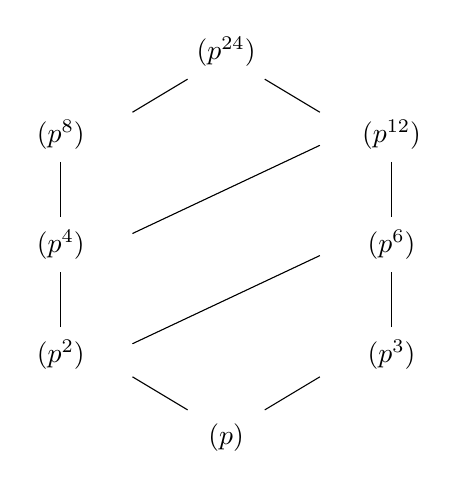
\begin{tikzpicture}[scale=0.7] %Replaced figure with tikz figure - TWJ 8/20/2010


\draw  (1.7,2.4) -- (0.7,3);
\draw  (-1.7,2.4) -- (-0.7,3);
\draw  (1.7,-2.4) -- (0.7,-3);
\draw  (-1.7,-2.4) -- (-0.7,-3);

\draw (3,1.5) -- (3,0.5);
\draw (-3,1.5) -- (-3,0.5);
\draw (3,-1.5) -- (3,-0.5);
\draw (-3,-1.5) -- (-3,-0.5);

\draw (-1.7,0.2) -- (1.7,1.8);
\draw (-1.7,-1.8) -- (1.7,-0.2);

\node at (0, 3.5) {$\gf(p^{24})$};

\node at (3, 2) {$\gf(p^{12})$};
\node at (3, 0) {$\gf(p^{6})$};
\node at (3, -2) {$\gf(p^{3})$};

\node at (-3, 2) {$\gf(p^{8})$};
\node at (-3, 0) {$\gf(p^{4})$};
\node at (-3, -2) {$\gf(p^{2})$};

\node at (0, -3.5) {$\gf(p)$};

\end{tikzpicture}
\end{center}
\caption{Subfields of $\gf(p^{24})$}
\label{FieldLattice}
\end{figure}

\end{example}
 


With each field $F$ we have a multiplicative group of nonzero elements of $F$ which we will denote by $F^*$\label{ntmultgrp}.   The multiplicative group of any finite field is cyclic.  This result follows from the more general result that we will prove in the next theorem. 

\begin{theorem}\label{finite:mult_group_theorem}
If $G$ is a finite  subgroup of $F^\ast$, the multiplicative group of nonzero elements of a field $F$, then $G$ is cyclic. 
\end{theorem}
 

\begin{proof}
Let $G$ be a finite subgroup of $F^\ast$ of order $n$.  By the Fundamental Theorem of Finite Abelian Groups (Theorem \ref{struct:Finite_Abelian_Grps_Theorem}),  
\[
G \cong {\mathbb Z}_{p_1^{e_1}} \times \cdots \times {\mathbb Z}_{p_k^{e_k}},
\]
where $n = p_1^{e_1} \cdots p_k^{e_k}$ and the  $p_1, \ldots, p_k$ are (not necessarily distinct) primes.
Let $m$ be the least common multiple of $p_1^{e_1}, \ldots, p_k^{e_k}$.  Then $G$ contains an element of order $m$.  Since every $\alpha$ in $G$ satisfies $x^r - 1$ for some $r$ dividing $m$, $\alpha$ must also be a root of $x^m - 1$.  Since $x^m -1$ has at most $m$ roots in $F$, $n \leq m$.  On the other hand, we know that $m \leq |G|$; therefore, $m = n$. Thus, $G$ contains an element of order $n$ and must be cyclic. 
\end{proof}

%Rewrote the first part of the proof.  Suggested by R. Beezer.
%TWK - 24/4/2013

\begin{corollary}\label{finite:cyclic_corollary}
The multiplicative group of all nonzero elements of a finite field is cyclic. 
\end{corollary}

\begin{corollary}\label{finite:finite_extension_corollary}
Every finite extension $E$ of a finite field $F$ is a simple extension of $F$. 
\end{corollary}

\begin{proof}
Let $\alpha$ be a generator for the cyclic group $E^{\ast}$ of nonzero elements of $E$. Then $E = F( \alpha )$. 
\end{proof}
 

\begin{example}{GF_2^4}
The finite field $\gf(2^4)$ is isomorphic to the field ${\mathbb Z}_2/ \langle 1 + x + x^4 \rangle$. Therefore, the elements of  $\gf(2^4)$ can be taken to be
\[
\{
a_0 + a_1 \alpha + a_2 \alpha^2 + a_3 \alpha^3 : a_i \in {\mathbb Z}_2
\text{ and } 1 + \alpha + \alpha^4 = 0
\}.
\]
Remembering that $1 + \alpha +\alpha^4 = 0$, we add and multiply elements of $\gf(2^4)$ exactly as we add and multiply polynomials.  The multiplicative group of $\gf(2^4)$ is isomorphic to ${\mathbb  Z}_{15}$ with generator $\alpha$: 
\[
\begin{array}{rclcrclcrcl}
\alpha^1 & = & \alpha & &
\alpha^6  & = & \alpha^2 + \alpha^3 & &
\alpha^{11} & = & \alpha + \alpha^2 + \alpha^3 \\
\alpha^2 & = & \alpha^2 & &
\alpha^7  & = & 1 + \alpha + \alpha^3 & &
\alpha^{12} & = & 1 + \alpha + \alpha^2 + \alpha^3 \\
\alpha^3 & = & \alpha^3 & &
\alpha^8  & = & 1 + \alpha^2 & &
\alpha^{13} & = & 1 + \alpha^2 + \alpha^3 \\
\alpha^4 & = & 1 + \alpha & &
\alpha^9  & = & \alpha + \alpha^3 & &
\alpha^{14} & = & 1 + \alpha^3 \\
\alpha^5 & = & \alpha + \alpha^2 & &
\alpha^{10}  & = & 1 + \alpha + \alpha^2 & &
\alpha^{15} & = & 1. 
\end{array}
\]
\end{example}


\section{Polynomial Codes}

%TWJ 2012/11/21
%Chapter reference updated.  Suggested by J. Buller.

With knowledge of polynomial rings and finite fields, it is now possible to derive more sophisticated codes than those of Chapter~\ref{algcodes}.  First let us recall that an $(n, k)$-block code consists of a one-to-one encoding function $E:{\mathbb Z}^{k}_{2} \rightarrow {\mathbb Z}^{n}_{2}$ and a decoding function $D:{\mathbb Z}^{n}_{2} \rightarrow {\mathbb Z}^{k}_{2}$.  The code is error-correcting if $D$ is onto.  A code is a linear code if it is the null space of a matrix $H \in {\mathbb M}_{k \times n}({\mathbb Z}_2)$.  

We are interested in a class of codes known as cyclic codes\index{Code!cyclic}.  Let $\phi : {\mathbb Z}_2^k \rightarrow {\mathbb  Z}_2^n$ be a binary $(n,k)$-block code.  Then $\phi$ is a \boldemph{cyclic code} if for every codeword $(a_1, a_2, \ldots, a_n )$, the cyclically shifted $n$-tuple $(a_n, a_1, a_2, \ldots, a_{n-1} )$ is also a codeword.  Cyclic codes are particularly easy to implement on a  computer using shift registers [2, 3].  


\begin{example}{6-3-linear_code}
Consider the $(6,3)$-linear codes generated by the two matrices
\[
G_1 
= 
\begin{pmatrix}
1 & 0 & 0 \\
0 & 1 & 0 \\
0 & 0 & 1 \\
1 & 0 & 0 \\
0 & 1 & 0 \\
0 & 0 & 1 
\end{pmatrix}
\quad
\text{and}
\quad
G_2 = 
\begin{pmatrix}
1 & 0 & 0 \\
1 & 1 & 0 \\
1 & 1 & 1 \\
1 & 1 & 1 \\
0 & 1 & 1 \\
0 & 0 & 1
\end{pmatrix}.
\]
Messages in the first code are encoded as follows:
\[
\begin{array}{rclccrcl}
(000) & \mapsto & (000000) & & & (100) & \mapsto & (100100) \\
(001) & \mapsto & (001001) & & & (101) & \mapsto & (101101) \\
(010) & \mapsto & (010010) & & & (110) & \mapsto & (110110) \\
(011) & \mapsto & (011011) & & & (111) & \mapsto & (111111).
\end{array}
\]
It is easy to see that the codewords form a cyclic code.  In the second code, 3-tuples are encoded in the following manner:
\[
\begin{array}{rclccrcl}
(000) & \mapsto & (000000) & & & (100) & \mapsto & (111100) \\
(001) & \mapsto & (001111) & & & (101) & \mapsto & (110011) \\
(010) & \mapsto & (011110) & & & (110) & \mapsto & (100010) \\
(011) & \mapsto & (010001) & & & (111) & \mapsto & (101101).
\end{array}
\]
This code cannot be cyclic, since $(101101)$ is a codeword but $(011011)$ is not a codeword.
\end{example}


\subsection*{Polynomial Codes}

We would like to find an easy method of obtaining cyclic linear codes.  To accomplish this, we can use our knowledge of finite fields and  polynomial rings over ${\mathbb Z}_2$.  Any binary $n$-tuple can be
interpreted as a polynomial in ${\mathbb Z}_2[x]$.  Stated another way, the $n$-tuple $(a_0, a_1, \ldots, a_{n-1} )$ corresponds to the polynomial
\[
f(x) = a_0 +  a_1 x +  \cdots + a_{n-1} x^{n-1},
\]
where the degree of $f(x)$ is at most $n-1$.   For example, the polynomial corresponding to the 5-tuple $(10011)$ is  
\[
1 + 0 x + 0 x^2 + 1 x^3 + 1 x^4 = 1 + x^3 + x^4.
\]
Conversely, with any polynomial $f(x) \in {\mathbb Z}_2[x]$ with $\deg f(x) < n$ we can associate a binary $n$-tuple.  The polynomial $x + x^2 + x^4$ corresponds to the 5-tuple $(01101)$.

Let us fix a nonconstant polynomial $g(x)$ in ${\mathbb Z}_2[x]$ of degree \mbox{$n - k$}.  We can define an $(n,k)$-code $C$ in the following manner.  If $(a_0, \ldots, a_{k-1})$ is a $k$-tuple to be encoded, then $f(x) = a_0 + a_1 x +  \cdots + a_{k-1} x^{k-1}$ is the corresponding polynomial
in ${\mathbb Z}_2[x]$.  To encode $f(x)$, we multiply by $g(x)$.  The codewords in $C$ are all those polynomials in ${\mathbb Z}_2[x]$ of degree less than  $n$ that are divisible by $g(x)$.  Codes obtained in this manner are called \boldemph{polynomial codes}\index{Polynomial!code}\index{Code!polynomial}.  


\begin{example}{generator_63-code}
If we let $g(x)= 1 + x^3$, we can define a $(6,3)$-code $C$ as follows.  To encode a 3-tuple $( a_0, a_1, a_2 )$, we multiply the corresponding polynomial $f(x) = a_0 + a_1 x + a_2 x^2$ by $1 + x^3$.  We are defining a map $\phi : {\mathbb Z}_2^3 \rightarrow {\mathbb Z}_2^6$ by $\phi  : f(x) \mapsto g(x) f(x)$.  It is easy to check that this map is a group homomorphism.  In fact, if we regard ${\mathbb Z}_2^n$ as a vector space over ${\mathbb Z}_2$, $\phi$ is a linear transformation of vector spaces (see Exercise~\ref{vect:linear_transformation}, Chapter~\ref{vect}).  Let us compute the kernel of $\phi$.  Observe that $\phi ( a_0, a_1, a_2 ) = (000000)$ exactly when 
\begin{align*}
0 + 0x + 0x^2 + 0x^3 + 0x^4 + 0 x^5 
& = (1 + x^3) ( a_0 + a_1 x + a_2 x^2 ) \\ 
& = a_0 + a_1 x + a_2 x^2 + a_0 x^3 + a_1 x^4 + a_2 x^5.
\end{align*}
Since the polynomials over a field form an integral domain, $a_0 + a_1 x + a_2 x^2$ must be the zero polynomial. Therefore, $\ker \phi = \{ (000) \}$ and $\phi$ is one-to-one. 
 

To calculate a generator matrix for $C$, we merely need to examine the way the polynomials $1$, $x$, and $x^2$ are encoded:
\begin{align*}
(1 + x^3) \cdot 1 & = 1 + x^3 \\
(1 + x^3)x & = x + x^4 \\
(1 + x^3)x^2 & = x^2 + x^5. 
\end{align*}  %Changed minimal polynomial from  (1 + x^3)x^3 & = x^2 + x^5 to (1 + x^3)x^2 & = x^2 + x^5.  Discovered by Jon Buller - TWJ 3/25/2011
We obtain the code corresponding to the generator matrix $G_1$ in Example~\ref{example:finite:6-3-linear_code}.  The parity-check matrix for this code is
\[
H
= 
\begin{pmatrix}
1 & 0 & 0 & 1 & 0 & 0 \\
0 & 1 & 0 & 0 & 1 & 0 \\
0 & 0 & 1 & 0 & 0 & 1 
\end{pmatrix}.
\]
Since the smallest weight of any nonzero codeword is 2, this code has the ability to detect all single errors.  
\end{example}


Rings of polynomials have a great deal of structure; therefore, our immediate goal is to establish a link between polynomial codes and ring theory. Recall that $x^n - 1 = (x - 1)( x^{n-1} + \cdots + x + 1)$.  The factor ring 
\[
R_n = {\mathbb Z}_2[x]/ \langle x^n - 1 \rangle
\]
can be considered to be the ring of polynomials of the form 
\[
f(t) = a_0 + a_1 t + \cdots + a_{n-1} t^{n-1}
\]
that satisfy the condition $t^n = 1$.  It is an easy exercise to show that ${\mathbb Z}_2^n$ and $R_n$ are isomorphic as vector spaces.  We will often identify elements in ${\mathbb Z}_2^n$ with elements in
${\mathbb Z}[x] / \langle x^n - 1 \rangle$.  In this manner we can interpret a linear code as a subset of ${\mathbb Z}[x] / \langle x^n - 1 \rangle$.  

The additional ring structure on polynomial codes is very powerful in describing cyclic codes. A cyclic shift of an $n$-tuple can be described by polynomial multiplication.  If $f(t) = a_0 + a_1 t + \cdots + a_{n-1} t^{n-1}$ is a code polynomial in $R_n$, then
\[
tf(t) = a_{n-1} + a_0 t + \cdots + a_{n-2} t^{n-1}
\]
is the cyclically shifted word obtained from multiplying $f(t)$ by $t$.  The following theorem gives a beautiful classification of cyclic codes in terms of the ideals of $R_n$.

\begin{theorem} \label{finite:cyclic_code_theorem}
A linear code $C$ in ${\mathbb Z}_2^n$ is cyclic if and only if it is an ideal in $R_n = {\mathbb Z}[x] / \langle x^n - 1 \rangle$. 
\end{theorem}
 
\begin{proof}
Let $C$ be a linear cyclic code and suppose that $f(t)$ is in $C$.  Then $t f(t)$ must also be in $C$. Consequently, $t^k f(t)$ is in $C$ for all $k \in {\mathbb N}$.  Since $C$ is a linear code, any linear combination of the codewords $f(t), tf(t), t^2f(t), \ldots, t^{n-1}f(t)$ is also a codeword; therefore, for every polynomial $p(t)$, $p(t)f(t)$ is in $C$.  Hence, $C$ is an ideal. 

Conversely, let $C$ be an ideal in ${\mathbb Z}_2[x]/\langle x^n + 1\rangle$. Suppose that $f(t) = a_0 + a_1 t + \cdots + a_{n - 1} t^{n - 1}$ is a codeword in $C$.  Then $t f(t)$ is a codeword in $C$; that is, $(a_1, \ldots, a_{n-1}, a_0)$ is in $C$.
\end{proof} 

\medskip

Theorem~\ref{finite:cyclic_code_theorem} tells us that knowing the ideals of $R_n$ is equivalent to knowing the linear cyclic codes in ${\mathbb Z}_2^n$.  Fortunately, the ideals in $R_n$ are easy to describe.  The  natural ring homomorphism $\phi : {\mathbb Z}_2[x] \rightarrow R_n$ defined by $\phi[f(x)] = f(t)$ is a surjective homomorphism.  The kernel of $\phi$ is the ideal generated by $x^n - 1$.  By Theorem~\ref{rings:correspond_theorem}, every ideal $C$ in $R_n$ is of the form $\phi(I)$, where $I$ is an ideal in ${\mathbb Z}_2[x]$ that contains $\langle x^n - 1 \rangle$.  By Theorem~\ref{poly:PI_theorem}, we know that every ideal $I$ in ${\mathbb Z}_2[x]$ is a principal ideal, since ${\mathbb Z}_2$ is a field. Therefore, $I = \langle g(x) \rangle$ for some unique monic polynomial in ${\mathbb Z}_2[x]$. Since $\langle x^n - 1 \rangle$ is contained in $I$, it must be the case that $g(x)$ divides $x^n - 1$. Consequently, every ideal $C$ in $R_n$ is of the form 
\[
C= \langle g(t) \rangle = \{ f(t)g(t) : f(t) \in R_n \mbox{ and $g(x)
\mid (x^n - 1)$ in } {\mathbb Z}_2[x] \}.
\]
The unique monic polynomial of the smallest degree that generates $C$ is called the \boldemph{minimal generator polynomial}\index{Minimal generator polynomial}\index{Polynomial!minimal generator} of $C$. 


\begin{example}{factor_x7-1}
If we factor $x^7 - 1$ into irreducible components, we have
\[
x^7 - 1 = (1 + x)(1 + x + x^3)(1+ x^2 + x^3).
\]
We see that $g(t) = (1 + t + t^3)$ generates an ideal $C$ in $R_7$.  This code is a $(7, 4)$-block code.  As in Example~\ref{example:finite:generator_63-code}, it is easy to calculate a generator matrix by examining what $g(t)$ does to the polynomials 1, $t$, $t^2$, and $t^3$.  A generator matrix for $C$ is 
\[
G =
\begin{pmatrix}
1 & 0 & 0 & 0 \\
1 & 1 & 0 & 0 \\
0 & 1 & 1 & 0 \\
1 & 0 & 1 & 1 \\
0 & 1 & 0 & 1 \\
0 & 0 & 1 & 0 \\
0 & 0 & 0 & 1
\end{pmatrix}.
\]
\end{example}

 
In general, we can determine a generator matrix for an $(n, k)$-code $C$ by the manner in which the elements $t^k$ are encoded. Let $x^n - 1 = g(x) h(x)$ in ${\mathbb Z}_2[x]$. If $g(x) = g_0 + g_1 x + \cdots + g_{n-k} x^{n-k}$ and $h(x) = h_0 + h_1 x +  \cdots + h_k x^k$, then the $n \times k$ matrix
\[
G = 
\begin{pmatrix}
g_0 & 0   & \cdots & 0 \\
g_1 & g_0 & \cdots & 0 \\
\vdots & \vdots &\ddots & \vdots \\
g_{n-k}   & g_{n-k-1} & \cdots & g_0 \\
0   & g_{n-k} & \cdots & g_{1} \\
\vdots & \vdots & \ddots & \vdots \\
0   & 0 & \cdots & g_{n-k}
\end{pmatrix}
\]
is a generator matrix for the code $C$ with generator polynomial $g(t)$.  The parity-check matrix for $C$ is the $(n-k) \times n$ matrix 
\[
H =
\begin{pmatrix}
0   & \cdots & 0   & 0      & h_k    & \cdots & h_0 \\
0   & \cdots & 0 & h_k & \cdots & h_0    & 0 \\
\cdots  & \cdots & \cdots  & \cdots &  \cdots &  \cdots & \cdots \\
h_k & \cdots & h_0 & 0      & 0      & \cdots & 0 
\end{pmatrix}.
\]
We will leave the details of the proof of the following proposition as an exercise.  

\begin{proposition}
Let $C = \langle g(t) \rangle$ be a cyclic code in $R_n$ and suppose that $x^n - 1 = g(x) h(x)$.  Then $G$ and $H$ are generator and parity-check matrices  for $C$, respectively.  Furthermore, $HG = 0$. 
\end{proposition}


\begin{example}{parity-check}
In Example~\ref{example:finite:factor_x7-1},
\[
x^7 - 1 = g(x) h(x) = (1 + x + x^3)(1 + x + x^2 + x^4).
\]
Therefore, a parity-check matrix for this code is
\[
H =
\begin{pmatrix}
0 & 0 & 1 & 0 & 1 & 1 & 1 \\
0 & 1 & 0 & 1 & 1 & 1 & 0 \\
1 & 0 & 1 & 1 & 1 & 0 & 0
\end{pmatrix}.
\]
\end{example}


To determine the error-detecting and error-correcting capabilities of a cyclic code, we need to know something about determinants.  If $\alpha_1, \ldots, \alpha_n$ are elements in a field $F$, then the $n 
\times n$ matrix  
\[
\begin{pmatrix}
1          & 1          & \cdots & 1 \\
\alpha_1   & \alpha_2   & \cdots & \alpha_n \\
\alpha_1^2 & \alpha_2^2 & \cdots & \alpha_n^2 \\
\vdots     & \vdots     & \ddots & \vdots \\
\alpha_1^{n-1} & \alpha_2^{n-1} & \cdots & \alpha_n^{n-1} 
\end{pmatrix}
\]
is called the \boldemph{Vandermonde matrix}\index{Vandermonde matrix}\index{Matrix, Vandermonde}.  The
determinant of this matrix is called the \boldemph{Vandermonde determinant}\index{Vandermonde determinant}\index{Determinant, Vandermonde}.  We will need the following lemma in our investigation of cyclic codes.

\begin{lemma}\label{finite:V_det_lemma}
Let $\alpha_1, \ldots, \alpha_n$ be elements in a field $F$ with $n \geq 2$.  Then
\[
\det
\begin{pmatrix}
1              & 1              & \cdots & 1 \\
\alpha_1       & \alpha_2       & \cdots & \alpha_n \\
\alpha_1^2     & \alpha_2^2     & \cdots & \alpha_n^2 \\
\vdots         & \vdots         & \ddots & \vdots \\
\alpha_1^{n-1} & \alpha_2^{n-1} & \cdots & \alpha_n^{n-1} 
\end{pmatrix}
= 
\prod_{1 \leq j < i \leq n} (\alpha_i - \alpha_j).
\]
In particular, if the $\alpha_i$'s are distinct, then the determinant is nonzero.
\end{lemma}


\begin{proof}
We will induct on $n$. If $n = 2$, then the determinant is $\alpha_2 - \alpha_1$.  Let us assume the result for $n  - 1$ and consider the polynomial $p(x)$ defined~by
\[
p(x)
=
\det
\begin{pmatrix}
1              & 1              & \cdots & 1              & 1 \\
\alpha_1       & \alpha_2       & \cdots & \alpha_{n-1}   & x \\
\alpha_1^2     & \alpha_2^2     & \cdots & \alpha_{n-1}^2 & x^2 \\
\vdots         & \vdots         & \ddots & \vdots         & \vdots \\
\alpha_1^{n-1} & \alpha_2^{n-1} & \cdots & \alpha_{n-1}^{n-1} & x^{n-1}
\end{pmatrix}.
\]
Expanding this determinant by cofactors on the last column, we see that $p(x)$ is a polynomial of at most degree $n-1$.  Moreover, the roots of $p(x)$ are $\alpha_1, \ldots, \alpha_{n-1}$, since the substitution of any one of these elements in the last column will produce a column identical to the last column in the matrix.  Remember that the determinant of a matrix is zero if it has two identical columns. Therefore,     
\[
p(x) = (x - \alpha_1)(x - \alpha_2) \cdots (x - \alpha_{n-1}) \beta, 
\]
where
\[
\beta = (-1)^{n+n}
\det
\begin{pmatrix}
1              & 1              & \cdots & 1 \\
\alpha_1       & \alpha_2       & \cdots & \alpha_{n-1} \\
\alpha_1^2     & \alpha_2^2     & \cdots & \alpha_{n-1}^2 \\
\vdots         & \vdots         & \ddots & \vdots \\
\alpha_1^{n-2} & \alpha_2^{n-2} & \cdots & \alpha_{n-1}^{n-2} 
\end{pmatrix}.
\]
By our induction hypothesis,
\[
\beta = (-1)^{n+n} \prod_{1 \leq j < i \leq n-1} (\alpha_i - \alpha_j).
\]
If we let $x = \alpha_n$, the result now follows immediately.
\end{proof}

\medskip

The following theorem gives us an estimate on the error detection and correction capabilities for a particular generator polynomial.

\begin{theorem}\label{finite:min_dist_theorem}
Let $C = \langle g(t) \rangle$ be a cyclic code in $R_n$ and suppose that $\omega$ is a primitive $n$th root of unity over ${\mathbb Z}_2$.  If $s$ consecutive powers of $\omega$ are roots of $g(x)$, then the minimum distance of $C$ is at least $s+1$.
\end{theorem}


\begin{proof}
Suppose that 
\[
g( \omega^r) = g(\omega^{r+1}) = \cdots = g( \omega^{r+s-1}) = 0.
\]
Let $f(x)$ be some polynomial in $C$ with $s$ or fewer nonzero coefficients.  We can assume that 
\[
f(x) = a_{i_0} x^{i_0} + a_{i_1} x^{i_1} + \cdots + a_{i_{s-1}}
x^{i_{s-1}} 
\]
be some polynomial in $C$. It will suffice to show that all of the $a_i$'s must be 0.  Since 
\[
g( \omega^r) = g(\omega^{r+1}) = \cdots = g( \omega^{r+s-1}) = 0
\]
and $g(x)$ divides $f(x)$,
\[
f( \omega^r) = f(\omega^{r+1}) = \cdots = f( \omega^{r+s-1}) = 0.
\]
Equivalently, we have the following system of equations:
\begin{align*}
a_{i_0} (\omega^r)^{i_0} + a_{i_1} (\omega^r)^{i_1} + \cdots +
a_{i_{s-1}} (\omega^r)^{i_{s-1}} & = 0 \\ 
a_{i_0} (\omega^{r+1})^{i_0} + a_{i_1} (\omega^{r+1})^{i_2} + \cdots +
a_{i_{s-1}} (\omega^{r+1})^{i_{s-1}} & = 0 \\ 
& \vdots  \\
a_{i_0} (\omega^{r+s-1})^{i_0} + a_{i_1} (\omega^{r+s-1})^{i_1} +
\cdots + a_{i_{s-1}} (\omega^{r+s-1})^{i_{s-1}} & = 0.
\end{align*}
Therefore, $(a_{i_0}, a_{i_1}, \ldots, a_{i_{s-1}})$ is a solution to the homogeneous system of linear equations
\begin{align*}
(\omega^{i_0})^r x_0 + (\omega^{i_1})^r x_1 + \cdots +
(\omega^{i_{s-1}})^r x_{n-1} & = 0 \\ 
(\omega^{i_0})^{r+1} x_0 + (\omega^{i_1})^{r+1} x_1 + \cdots +
(\omega^{i_{s-1}})^{r+1} x_{n-1} & = 0 \\ 
& \vdots  \\
(\omega^{i_0})^{r+s-1} x_0 + (\omega^{i_1})^{r+s-1} x_1 + \cdots +
(\omega^{i_{s-1}})^{r+s-1} x_{n-1} & = 0.
\end{align*}
However, this system has a unique solution, since the determinant of the matrix
\[
\begin{pmatrix}
(\omega^{i_0})^r & (\omega^{i_1})^r & \cdots & (\omega^{i_{s-1}})^r \\
(\omega^{i_0})^{r+1} & (\omega^{i_1})^{r+1} & \cdots &
(\omega^{i_{s-1}})^{r+1} \\
\vdots & \vdots         & \ddots & \vdots \\
(\omega^{i_0})^{r+s-1} & (\omega^{i_1})^{r+s-1} & \cdots &
(\omega^{i_{s-1}})^{r+s-1} 
\end{pmatrix}
\]
can be shown to be nonzero using Lemma~\ref{finite:V_det_lemma} and the basic properties of determinants (Exercise).   Therefore, 
this solution must be $a_{i_0} = a_{i_1} = \cdots = a_{i_{s-1}} = 0$.  
\end{proof}


\subsection*{BCH Codes}
 
Some of the most important codes,
discovered independently by A.~Hocquenghem in 1959 and by R.~C. Bose and D.~V. Ray-Chaudhuri in 1960, are BCH codes.  The European and transatlantic  communication systems both use BCH codes.  Information words to be
encoded are of length 231, and a polynomial of degree 24 is used to
generate the code.  Since $231 + 24 = 255 = 2^8-1$, we are dealing
with a \mbox{$(255, 231)$-block} code. This BCH code will detect six
errors and has a failure rate of 1 in 16 million. One advantage of BCH
codes is that efficient error correction algorithms exist for them. 


The idea behind BCH codes is to choose a generator polynomial of
smallest degree that has the largest error detection and error
correction 
capabilities. Let $d = 2r + 1$ for some $r \geq 0$.  Suppose that
$\omega$ is a primitive $n$th root of unity over ${\mathbb Z}_2$, and
let $m_i(x)$ be the minimal polynomial over ${\mathbb Z}_2$ of
$\omega^i$. If  
\[
g(x) = \lcm[ m_1(x), m_{2}(x), \ldots, m_{2r}(x)],
\]
then the cyclic code $\langle g(t) \rangle$ in $R_n$ is called the
\boldemph{BCH code of length}\index{Code!BCH} $n$ \boldemph{and distance} $d$.
By Theorem~\ref{finite:min_dist_theorem}, the minimum distance of $C$ is at least $d$. 


\begin{theorem}
Let $C = \langle g(t) \rangle$ be a cyclic code in $R_n$. The
following statements are equivalent. 
\begin{enumerate}

\rm\item\it
The code $C$ is a BCH code whose minimum distance is at least $d$.


\rm\item\it
A code polynomial $f(t)$ is in $C$ if and only if $f( \omega^i) = 0$
for $1 \leq i < d$. 

\rm\item\it
The matrix 
\[
H
=
\begin{pmatrix}
1      & \omega      & \omega^2    & \cdots & \omega^{n-1}\\
1      & \omega^2    & \omega^{4}  & \cdots & \omega^{(n-1)(2)} \\
1      & \omega^3    & \omega^{6}  & \cdots & \omega^{(n-1)(3)} \\
\vdots & \vdots      & \vdots      & \ddots & \vdots \\
1      & \omega^{2r} & \omega^{4r} & \cdots & \omega^{(n-1)(2r)} 
\end{pmatrix}
\]
is a parity-check matrix for $C$.

\end{enumerate}
\end{theorem}


\begin{proof}
(1) $\Rightarrow$ (2).
If $f(t)$ is in $C$, then $g(x) \mid f(x)$ in ${\mathbb Z}_2[x]$. Hence,
for $i = 1, \ldots, 2r$, $f( \omega^i) = 0$ since $g( \omega^i ) =
0$. Conversely, suppose that $f( \omega^i) = 0$ for $1 \leq i \leq d$.
Then $f(x)$ is divisible by each $m_i(x)$, since $m_i(x)$ is the
minimal polynomial of $\omega^i$. Therefore, $g(x) \mid f(x)$ by the
definition of $g(x)$. Consequently, $f(x)$ is a codeword.


(2) $\Rightarrow$ (3).
Let \mbox{$f(t) = a_0 + a_1 t + \cdots + a_{n-1}v t^{n-1}$} be in $R_n$. The
corresponding $n$-tuple in ${\mathbb Z}_2^n$ is ${\mathbf x} = (a_0 a_1
\cdots a_{n-1})^{\rm t}$. By (2),
\[
H {\mathbf x}
=
\begin{pmatrix}
a_0 + a_1 \omega + \cdots + a_{n-1} \omega^{n-1} \\
a_0 + a_1 \omega^2 + \cdots + a_{n-1} (\omega^2)^{n-1} \\
\vdots \\
a_0 + a_1 \omega^{2r} + \cdots + a_{n-1} (\omega^{2r})^{n-1}
\end{pmatrix}
=
\begin{pmatrix}
f(\omega) \\
f(\omega^2) \\
\vdots \\
f(\omega^{2r})
\end{pmatrix}
=0
\]
exactly when $f(t)$ is in $C$. Thus, $H$ is a parity-check matrix for
$C$.

(3) $\Rightarrow$ (1).
By (3), a code polynomial $f(t) = a_0 + a_1 t + \cdots + a_{n-1}
t^{n-1}$ is in $C$ exactly when $f(\omega^i) = 0$ for $i = 1, \ldots,
2r$. The smallest such polynomial is $g(t) = \lcm[ m_1(t),\ldots,
m_{2r}(t)]$.  Therefore, $C = \langle g(t) \rangle$.
\end{proof}



\begin{example}{x15-1}
It is easy to verify that $x^{15} - 1 \in {\mathbb Z}_2[x]$ has a
factorization
\[
x^{15} - 1 = (x + 1)(x^2 + x + 1)(x^4 + x + 1)(x^4 + x^3 + 1)(x^4 +
x^3 + x^2 + x + 1),
\]
where each of the factors is an irreducible polynomial.
Let $\omega$ be a root of $1 + x + x^4$. The Galois field $\gf(2^4)$ is
\[
\{
a_0 + a_1 \omega + a_2 \omega^2 + a_3 \omega^3 : a_i \in {\mathbb Z}_2
\mbox{ and } 1 + \omega + \omega^4 = 0
\}.
\]
By Example~\ref{example:finite:GF_2^4}, $\omega$ is a primitive 15th root of unity. The
minimal polynomial of $\omega$ is $m_1(x) = 1 + x + x^4$. It is easy
to see that $\omega^2$ and $\omega^4$ are also roots of $m_1(x)$. The
minimal polynomial of $\omega^3$ is $m_2(x) = 1 + x + x^2 + x^3 +
x^4$. Therefore, 
\[
g(x) = m_1(x) m_2(x) = 1 + x^4 + x^6 + x^7 + x^8
\]
has roots $\omega$, $\omega^2$, $\omega^3$, $\omega^4$.  Since both $m_1(x)$
and $m_2(x)$ divide $x^{15} - 1$, the BCH code is a $(15, 7)$-code. If
$x^{15} -1 = g(x)h(x)$, then $h(x) = 1 + x^4 + x^6 + x^7$; therefore,
a parity-check matrix for this code is
\[
\left( %This matrix is too large for pmatrix - TWJ 8/19/2010
\begin{array}{ccccccccccccccc}
0 & 0 & 0 & 0 & 0 & 0 & 0 & 1 & 1 & 0 & 1 & 0 & 0 & 0 & 1 \\
0 & 0 & 0 & 0 & 0 & 0 & 1 & 1 & 0 & 1 & 0 & 0 & 0 & 1 & 0 \\
0 & 0 & 0 & 0 & 0 & 1 & 1 & 0 & 1 & 0 & 0 & 0 & 1 & 0 & 0 \\
0 & 0 & 0 & 0 & 1 & 1 & 0 & 1 & 0 & 0 & 0 & 1 & 0 & 0 & 0 \\
0 & 0 & 0 & 1 & 1 & 0 & 1 & 0 & 0 & 0 & 1 & 0 & 0 & 0 & 0 \\
0 & 0 & 1 & 1 & 0 & 1 & 0 & 0 & 0 & 1 & 0 & 0 & 0 & 0 & 0 \\
0 & 1 & 1 & 0 & 1 & 0 & 0 & 0 & 1 & 0 & 0 & 0 & 0 & 0 & 0 \\
1 & 1 & 0 & 1 & 0 & 0 & 0 & 1 & 0 & 0 & 0 & 0 & 0 & 0 & 0
\end{array}
\right).
\]
\end{example}


 
\markright{EXERCISES}
\section*{Exercises}
\exrule

 
{\small
\begin{enumerate}

\item
Calculate each of the following.
\begin{multicols}{2}
\begin{enumerate}

\item 
$[\gf(3^6) : \gf(3^3)]$

\item 
$[\gf(128): \gf(16)]$

\item 
$[\gf(625) : \gf(25) ]$

\item 
$[\gf(p^{12}): \gf(p^2)]$


\end{enumerate}
\end{multicols}



\item
Calculate $[\gf(p^m): \gf(p^n)]$, where $n \mid m$.


\item
What is the lattice of subfields for $\gf(p^{30})$?


\item
Let $\alpha$ be a zero of $x^3 + x^2 + 1$ over ${\mathbb Z}_2$. 
Construct a finite field of order 8. Show that
$x^3 + x^2 + 1$ splits in ${\mathbb Z}_2(\alpha)$. 
 

\item
Construct a finite field of order 27.


\item
Prove or disprove: ${\mathbb Q}^\ast$ is cyclic.

 
\item
Factor each of the following polynomials in ${\mathbb Z}_2[x]$.
\begin{multicols}{2}
\begin{enumerate}

\item 
$x^5- 1$

\item 
$x^6 + x^5 + x^4 + x^3 + x^2 + x + 1$

\item 
$x^9 - 1$

\item 
$x^4 +x^3 + x^2 + x + 1$ 


\end{enumerate}
\end{multicols}



\item
Prove or disprove: ${\mathbb Z}_2[x] / \langle x^3 + x + 1 \rangle \cong
{\mathbb Z}_2[x] / \langle x^3 + x^2 + 1 \rangle$. 


\item
Determine the number of cyclic codes of length $n$ for $n = 6$, 7, 8,
10.


\item
Prove that the ideal $\langle t + 1 \rangle$ in $R_n$ is the code in
${\mathbb Z}_2^n$ consisting of all words of even parity.


\item
Construct all BCH codes of
\begin{multicols}{2}
\begin{enumerate}

\item
length 7.

\item
length 15.

\end{enumerate}
\end{multicols}



%************************THEORY********************



\item
Prove or disprove: There exists a finite field that is algebraically
closed. 


\item
Let $p$ be prime.  Prove that the field of rational functions ${\mathbb
Z}_p(x)$ is an infinite field of characteristic $p$.


\item
Let $D$ be an integral domain of characteristic $p$.  Prove that $(a -
b)^{p^n} = a^{p^n} - b^{p^n}$ for all $a, b \in D$.


\item
Show that every element in a finite field can be written as the sum
of two squares.




\item
Let $E$ and $F$ be subfields of a finite field $K$. If $E$ is
isomorphic to $F$, show that $E=F$.


\item
Let $F \subset E \subset K$ be fields. If $K$ is separable over $F$,
show that $K$ is also separable over $E$.


\item
Let $E$ be an extension of a finite field $F$, where $F$ has $q$
elements. Let $\alpha \in E$ be algebraic over $F$ of degree $n$.
Prove that $F( \alpha )$ has $q^n$ elements. 


\item
Show that every finite extension of a finite field $F$ is simple;
that is, if $E$ is a finite extension of a finite field $F$, prove
that there exists an $\alpha \in E$ such that $E = F( \alpha )$.


\item
Show that for every $n$ there exists an irreducible polynomial of 
degree $n$ in~${\mathbb Z}_p[x]$.



\item \label{exercise:finite:frobeniusmap}
Prove that the \boldemph{Frobenius map}\index{Frobenius map} $\phi : \gf(p^n) \rightarrow \gf(p^n)$ given by $\phi : \alpha \mapsto
\alpha^p$ is an automorphism of order $n$. 


\item
Show that every element in $\gf(p^n)$ can be written in the form
$a^p$ for some unique $a \in \gf(p^n)$.


\item
Let $E$ and $F$ be subfields of $\gf(p^n)$. If $|E| = p^r$ and
$|F| = p^s$, what is the order of $E \cap F$? 


\item
\textbf{Wilson's Theorem.}\index{Wilson's Theorem}
Let $p$ be prime.  Prove that $(p-1)! \equiv -1 \pmod{p}$. 


\item
If $g(t)$ is the minimal generator polynomial for a cyclic code $C$ in
$R_n$, prove that the constant term of $g(x)$ is $1$.


\item
Often it is conceivable that a burst of errors might occur during
transmission, as in the case of a power surge.  Such a momentary burst
of interference might alter several consecutive bits in a codeword.
Cyclic codes permit the detection of such error bursts. Let $C$ be an
$(n,k)$-cyclic code. Prove that any error burst up to $n-k$ digits can
be detected.  


\item
Prove that the rings $R_n$ and ${\mathbb Z}_2^n$ are isomorphic as vector
spaces. 


\item
Let $C$ be a code in $R_n$ that is generated by $g(t)$. If $\langle
f(t) \rangle$ is another code in $R_n$, show that $\langle g(t) \rangle
\subset \langle f(t) \rangle$ if and only if $f(x)$ divides $g(x)$ in
${\mathbb Z}_2[x]$.


\item
Let $C = \langle g(t) \rangle$ be a cyclic code in $R_n$ and suppose
that $x^n - 1 = g(x) h(x)$, where $g(x) = g_0 + g_1 x + \cdots +
g_{n-k} x^{n-k}$ and $h(x) = h_0 + h_1 x +  \cdots + h_k x^k$. Define
$G$ to be the $n \times k$ matrix
\[
G = 
\begin{pmatrix}
g_0 & 0   & \cdots & 0 \\
g_1 & g_0 & \cdots & 0 \\
\vdots & \vdots &\ddots & \vdots \\
g_{n-k}   & g_{n-k-1} & \cdots & g_0 \\
0   & g_{n-k} & \cdots & g_{1} \\
\vdots & \vdots & \ddots & \vdots \\
0   & 0 & \cdots & g_{n-k}
\end{pmatrix}
\]
and $H$ to be the $(n-k) \times n$ matrix 
\[
H =
\begin{pmatrix}
0   & \cdots & 0   & 0      & h_k    & \cdots & h_0 \\
0   & \cdots & 0   & h_k    & \cdots & h_0    & 0 \\
\cdots & \cdots & \cdots  & \cdots & \cdots & \cdots & \cdots  \\
h_k & \cdots & h_0 & 0      & 0      & \cdots & 0 
\end{pmatrix}.
\]
\begin{enumerate}

\item
Prove that $G$ is a generator matrix for $C$.

\item
Prove that $H$ is a parity-check matrix for $C$.


\item
Show that $HG = 0$.


\end{enumerate}







\end{enumerate}
}
 

 
\subsection*{Additional Exercises: Error Correction for BCH Codes}


{\small
BCH codes have very attractive error correction algorithms. Let $C$ be
a BCH code in $R_n$, and suppose that a code polynomial $c(t) = c_0 +
c_1 t + \cdots + c_{n-1} t^{n-1}$ is transmitted. Let $w(t) = w_0 +
w_1 t + \cdots w_{n-1} t^{n-1}$ be the polynomial in $R_n$ that is
received.  If errors have occurred in bits $a_1, \ldots, a_k$, then
$w(t) = c(t) + e(t)$, where $e(t) = t^{a_1} + t^{a_2} + \cdots +
t^{a_k}$ is the \boldemph{error polynomial}\index{Polynomial!error}. The
decoder must determine the integers $a_i$ and then recover $c(t)$ from
$w(t)$ by flipping the $a_i$th bit. From $w(t)$ we can compute
$w( \omega^i ) = s_i$ for $i = 1, \ldots, 2r$, where $\omega$ is a
primitive $n$th root of unity over ${\mathbb Z}_2$. We say the \boldemph{
syndrome}\index{Syndrome of a code} of $w(t)$ is $s_1, \ldots,
s_{2r}$. 
\begin{enumerate}

\item
Show that $w(t)$ is a code polynomial if and only if $s_i = 0$ for all
$i$. 

\item
Show that 
\[
s_i = w( \omega^i) = e( \omega^i) = \omega^{i a_1} + \omega^{i a_2} +
\cdots + \omega^{i a_k} 
\]
for $i = 1, \ldots, 2r$. The \boldemph{error-locator
polynomial}\index{Polynomial!error-locator} is defined to be 
\[
s(x) = (x + \omega^{a_1})(x + \omega^{a_2}) \cdots  (x +
\omega^{a_k}). 
\]

\item
Recall the $(15,7)$-block BCH code in Example~\ref{example:finite:parity-check}.  By Theorem~\ref{algecodes:min_distance_theorem}, this
code is capable of correcting two errors. Suppose that these errors
occur in bits $a_1$ and $a_2$. The error-locator polynomial
is $s(x) = (x + \omega^{a_1})(x + \omega^{a_2})$. Show that
\[
s(x) = x^2 + s_1 x + \left( s_1^2 + \frac{s_3}{s_1} \right).
\]


\item
Let $w(t) = 1 + t^2 +t^4 + t^5 + t^7 + t^{12} + t^{13}$. Determine
what the originally transmitted code polynomial was.

\end{enumerate}


}



\subsection*{References and Suggested Readings}
 

{\small

\begin{itemize}
 
\item[\textbf{[1]}] %Reference updated 5/4/2010 - TWJ
Childs, L. 
\textit{A Concrete Introduction to Higher Algebra}. 2nd ed.
Springer-Verlag, New York, 1995. .

\item[\textbf{[2]}] %No longer in print 8/20/2010 - TWJ
G{\aa}ding, L. and Tambour, T. \textit{Algebra for Computer
Science}. Springer-Verlag, New York, 1988.

\item[\textbf{[3]}] %Reference updated 8/20/2010 - TWJ
Lidl, R. and Pilz, G. 
\textit{Applied Abstract Algebra}. 2nd ed. Springer,
New York, 1998. 
An excellent presentation of finite
fields and their applications.

\item[\textbf{[4]}] %No longer in print 8/20/2010 - TWJ
Mackiw, G. \textit{Applications of Abstract Algebra}. Wiley,
New York, 1985.
 
\item[\textbf{[5]}]
Roman, S. \textit{Coding and Information Theory}. Springer-Verlag,
New York, 1992. 


\item[\textbf{[6]}] %Reference updated - TWJ 8/20/2010
van Lint, J. H. \textit{Introduction to Coding Theory}. Springer,
New York, 1999. 
\end{itemize}
}

\sagesection

   %Finite Fields
%%%%(c)
%%%%(c)  This file is a portion of the source for the textbook
%%%%(c)
%%%%(c)    Abstract Algebra: Theory and Applications
%%%%(c)    by Thomas W. Judson
%%%%(c)
%%%%(c)    Sage Material
%%%%(c)    Copyright 2011 by Robert A. Beezer
%%%%(c)
%%%%(c)  See the file COPYING.txt for copying conditions
%%%%(c)
%%%%(c)
\begin{sageverbatim}\end{sageverbatim}
%
\sageexercise{1}%
In the analysis of Example~\extref{example:galois:galois_x4-2}{7}{quartic subgroup lattice example} with Sage, two subgroups of order 2 and one subgroup of order 4 were not analyzed.  Determine the fixed fields of these three subgroups.
\begin{sageverbatim}\end{sageverbatim}
%
\sageexercise{2}%
Build the splitting field of $p(x)=x^3-6x^2+12x-10$ and then determine the Galois group of $p(x)$ as a concrete group of explicit permutations.  Build the lattice of subgroups of the Galois group, again using the same explicit permutations.  Using the fundamental theorem of Galois theory, construct the subfields of the splitting field.  Include your supporting documentation in your submitted Sage worksheet.  Also, submit a written component of this assignment containing a complete layout of the subgroups and subfields, written entirely with mathematical notation and with no Sage commands, designed to illustrate the correspondence between the two.  All you need here is the graphical layout, suitably labeled --- the Sage worksheet will substantiate your work.
\begin{sageverbatim}\end{sageverbatim}
%
\sageexercise{3}%
The polynomial $x^5-x-1$ has all of the symmetric group $S_5$ as its Galois group.  Because $S_5$ is not solvable, we know this polynomial to be an example of a quintic polynomial that is not solvable by radicals.  Unfortunately, asking Sage to compute this Galois group takes far too long.  So this exercise will simulate that experience with a slightly smaller example.\par
%
Consider the polynomial $p(x)=x^4+x+1$.\\
%
(a) Build the splitting field of $p(x)$ one root at a time.  Create an extension, factor there, discard linear factors, use the remaining irreducible factor to extend once more.  Repeat until $p(x)$ factors completely.  Be sure to do a final extension via just a linear factor.  This is a little silly, and Sage will seem to ignore your final generator (so you will want to setermine what it is equivalent to in terms of the previous gfenerators).  Directions below depend on taking this extra step.\\
%
(b) Factor the original polynomial over the final extension field in the tower.  What is boring about this factorization in comparison to some other examples we have done?\\
%
(c) Construct the full tower as an absolute field over ${\mathbb Q}$.  From the degree of this extension and the degree of the original polynomial, infer the Galois group of the polynomial.\\
%
(d) Using the mappings that allow you to translate between the tower and the absolute field (obtained from the \verb?.structure()? method), choose one of the roots (any one) and express it in terms of the single generator of the absolute field.  Then reverse the procedure and express the single generator of the absolute field in terms of the roots in the tower.\par
%
(e) Compute the group of automorphisms of the absolute field (but don't display the whole group in what you submit).  Take all four roots (including your silly one from the last step of the tower construction) and apply each field automorphism to the four roots (creating the guaranteed permutations of the roots).  Comment on what you see.\\
%
(f)  There is one nontrivial automorphism that has an especially simple form (it is the second one for me) when applied to the generator of the absolute field.  What does this automorphism do to the roots of $p(x)$?\\
%
(g)  Consider the extension of ${\mathbb Q}$ formed by adjoining just one of the roots.  This is a subfield of the splitting field of the polynomial, so is the fixed field of a subgroup of the Galois group.  Give a simple description of the corresponding subgroup using language we typically only apply to permutation groups.
\begin{sageverbatim}\end{sageverbatim}
%
\sageexercise{4}%
Return to the splitting field of the quintic discussed in the introduction to the previous problem ($x^5-x-1$).  Create the first two intermediate fields by adjoining two roots (one at a time).  But instead of factoring at each step to get a new irreducible polynomial, \emph{divide} by the linear factor you \emph{know} is a factor.  In general, the quotient might factor further, but in this exercise presume it does not.  In other words, act as if your quotient by the linear factor is irreducible.  If it is not, then the \texttt{NumberField} command should complain (which it won't).\par
%
After adjoining two roots, create the extension producing a third root, and do the division.  You should now have a quadratic factor.  Assuming the quadratic is irreducible (it is) argue that you have enough evidence to establish the order of the Galois group, and hence can determine \emph{exactly} which group it is.\par
%
You can try to use this quadratic factor to create one more step in the extensions, and you will arrive at the splitting field, as can be seen with logic or division.  However, this could take a long time to complete (save your work beforehand!).  You can try passing the \verb?check=False? argument to the \verb?NumberField? command --- this will bypass checking irreducibility.
\begin{sageverbatim}\end{sageverbatim}
%
\sageexercise{5}%
Create the finite field of order $3^6$, letting Sage supply the default polynomial for its construction.  The polynomial $x^6+x^2+2*x+1$ is irreducible over this finite field.  Check that this polynomial splits in the finite field, and then use the \verb?.roots()? method to collect the roots of the polynomial.  Get the group of automorphisms of the field with the \verb?End()? command.\par
%
You now have all of the pieces to associate each field automorphism with a permutation of the roots.  From this, identify the Galois group and all of its subgroups.  For each subgroup, determine the fixed field.  You might find the roots easier to work with if you use the \verb?.log()? method to identify them as powers of the field's multiplicative generator.\par
%
Your Galois group in this example will be abelian.  So every subgroup is normal, and hence any extension is also normal.  Can you give extend this example by choosing a nontrivial intermediate field with a nontrivial irreducible polynomial that has all of its roots in the intermediate field and a nontrivial irreducible polynomial with none of its roots in the intermediate field?
%
Your results here are ``typical'' in the sense that the particular field or irreducible polynomial makes little difference in the qualitative nature of the results.
\begin{sageverbatim}\end{sageverbatim}
%
\sageexercise{6}%
The splitting field for the irreducible polynomial $p(x)=x^7-7x+3$ has degree 168 (hence this is the order of the Galois group).  This polynomial is derived from an ``Elkies trinomial curve,'' a hyperelliptic curve (below) that produces polynomials with interesting Galois groups:
$$y^2 = x(81x^5 + 396x^4 + 738x^3 + 660x^2 + 269x + 48)$$\par
%
For $p(x)$ the resulting Galois group is $PSL(2,7)$, a simple group.  If $SL(2,7)$ is all $2\times 2$ matrices over ${\mathbb Z}_7$ with determinant 1, then $PSL(2,7)$ is the quotient by the subgroup $\{I_2,-I_2\}$.  It is the second-smallest non-abelian simple group (after $A_5$).\par
%
See how far you can get in using Sage to build this splitting field.  A degree 7 extension will yield one linear factor, and a subsequent degree 6 extension will yield two linear factors, leaving a quartic factor.  Here is where the computations begin to slow down.  If we believe that the splitting field has degree 168, then we know that adding a root from this degree 4 factor will get us to the splitting field.  Creating this extension may be possible computationally, but verifying that the quartic splits into linear factors here seems to be infeasible.
\begin{sageverbatim}\end{sageverbatim}
%
\sageexercise{7}%
Return to ~\extref{example:galois:galois_x4-2}{7}{quartic subgroup lattice example}, and the complete list of subfields obtainable from the \verb?.subfields()? method applied to the flattened tower.  As mentioned, these are technically not subfields, but do have embeddings into the tower.  Given two subfields, their respective primitive elements are embedded into the tower, with an image that is a linear combination of powers of the primitive element for the tower.\par
%
If one subfield is contained in the other, then the image of the primitive element for the smaller field should be a linear combination of the (appropriate) powers of the image of the primitive element for the larger field.  This is a linear algebra computation that should be possible in the tower, relative to the power basis for the whole tower.\par
%
Write a procedure to determine if two subfields are related by one being a subset of the other.  Then use this procedure to create the lattice of subfields.  The eventual goal would be a graphical display of the lattice, using the existing plotting facilities available for lattices, similar to the top half of Figure~\extref{Galois3}{23.3}{subfield diagram}.  This is a ``challenging'' exercise, which is code for ``it has not been tested.''
\begin{sageverbatim}\end{sageverbatim}
%

   %Galois Theory
%
% RAB, 2009/01/28
% Include GFDL as an appendix
%
% To build index with included sectioning info via "style file" execute:
%    makeindex -s aata-index-style.ist aata.idx
% See:  http://www.troubleshooters.com/linux/lyx/makeindex.htm
% Needs "\phantomsection", http://www.tug.org/applications/hyperref/manual.html
%
\backmatter
%%%%(c)
%%%%(c)  This file is a portion of the source for the textbook
%%%%(c)
%%%%(c)    Abstract Algebra: Theory and Applications
%%%%(c)    Copyright 1997 by Thomas W. Judson
%%%%(c)
%%%%(c)  See the file COPYING.txt for copying conditions
%%%%(c)
%%%%(c)
\chapter*{Hints and Solutions}
 
 
\addcontentsline{toc}{chapter}{Hints and Solutions}
\pagestyle{myheadings}
\markboth{HINTS AND SOLUTIONS}{HINTS AND SOLUTIONS}
 
 
 
\subsection*{Chapter 1. Preliminaries}
 
 
{\small
\begin{itemize}
 
\item[1.]
(a) $\{ 2 \}$.
(b) $\{ 5 \}$.
 
\item[2.]
(a) $\{ (a,1), (a,2), (a,3), (b,1), (b,2), (b,3), (c,1), (c,2),
(c,3) \}$. \\
(d) $\emptyset$.
 
\item[6.]
If $x \in A \cup (B \cap C)$, then either $x \in A$ or $x \in B \cap 
C$  $\Rightarrow x \in A \cup B \text{ and } A \cup C \Rightarrow x
\in (A \cup B) \cap (A \cup C) \Rightarrow  A \cup (B \cap C) \subset 
(A \cup B) \cap (A \cup C)$. 
 
Conversely, $x \in (A \cup B) \cap (A \cup C) \Rightarrow  x \in A 
\cup B \text{ and } A \cup C \Rightarrow x \in A  \text{ or } x \text{ is in
both } $B$ \text{ and } $C$  \Rightarrow x \in A \cup (B \cap C) \Rightarrow
(A \cup B) \cap (A \cup C) \subset A \cup (B \cap C)$. Hence, $A \cup 
(B \cap C) = (A \cup B) \cap (A \cup C)$. 
 
\item[10.]
$(A \cap B) \cup (A \setminus B) \cup (B \setminus A) = (A \cap B) \cup 
(A \cap B') \cup (B \cap A') = [A \cap (B \cup B')] \cup (B \cap A')
= A \cup (B \cap A') = (A \cup B) \cap (A \cup A') = A \cup B$.
 
 
\item[14.]
$A \setminus (B \cup C) = A \cap (B \cup C)'
= (A \cap A) \cap (B' \cap C')
= (A \cap B') \cap (A \cap C') = 
(A \setminus B) \cap (A \setminus C)$. 
 
\item[17.]
(a) Not a map. $f(2/3)$ is undefined. \\
(c) Not a map. $f(1/2) =3/4$ and $f(2/4)=3/8$.
 
\item[18.]
(a)  One-to-one but not onto. $f({\mathbb R} ) = \{ x \in {\mathbb R} : x
> 0 \}$. \\
(c) Neither one-to-one nor onto.
 
\item[20.]
(a) $f(n) = n + 1$.
 
\item[22.]
(a) Let $x, y \in A$. Then $g(f(x)) = (g \circ f)(x) = (g \circ
f)(y) = g(f(y)) \Rightarrow f(x) = f(y) \Rightarrow x = y$,  so $g
\circ f$ is one-to-one. \\
(b) Let $c \in C$, then $c = (g \circ f)(x) = g(f(x))$ for some
$x \in A$. Since $f(x) \in B$, $g$ is onto.
 
\item[23.]
$f^{-1}(x) = (x+1)/(x-1)$.
 
\item[24.]
(a)  Let $y \in f(A_1 \cup A_2) \Rightarrow$ there exists an $x
\in A_1 \cup A_2$ such that $f(x) = y \Rightarrow y \in f(A_1)$ or
$f(A_2) \Rightarrow y \in f(A_1) \cup f(A_2) \Rightarrow f(A_1 \cup A_2)
\subset f(A_1) \cup f(A_2)$.
 
Conversely, let $y \in f(A_1) \cup f(A_2) \Rightarrow y \in f(A_1)$ or
$f(A_2) \Rightarrow$ there exists an $x \in A_1$ or there exists an
$x \in A_2$ such that $f(x) = y \Rightarrow$ there exists an $x \in
A_1 \cup A_2$ such that $f(x) = y \Rightarrow f(A_1) \cup f(A_2)
\subset f(A_1 \cup A_2)$. Hence, $f(A_1 \cup A_2) = f(A_1) \cup f(A_2)$. 
 
\item[25.]
(a) Not an equivalence relation. Fails to be symmetric.\\
(b) Not an equivalence relation. Fails to be reflexive since 0 is not equivalent to itself.\\
(c) Not an equivalence relation. Fails to be transitive.

%Solution to (b) corrected.  Suggested by R. Nilange.
%TWJ 8/14/2013 


 
\item[28.]
Let $X = {\mathbb N} \cup \{ \sqrt{2}\, \}$ and define $x \sim y$ if $x + y
\in {\mathbb N}$.
 
\end{itemize}
}
 
 
 
\subsection*{Chapter 2. The Integers}
 
 
{\small
\begin{itemize}
 
 
\item[1.]
$S(1): [1(1+1)(2(1) + 1)]/6 = 1 = 1^2$ is true. Assume $S(k): 1^2 +2^2
+ \cdots + k^2 = [k(k+1)(2k+1)]/6$ is true. Then $1^2 + 2^2 + \cdots +
k^2 + (k+1)^2 = [k(k+1)(2k+1)]/6 + (k+1)^2 = [(k+1)((k+1) +1)(2(k+1) +
1)]/6$, so $S(k+1)$ is true. Thus $S(n)$ is true for all positive
integers $n$. 
 
\item[3.]
$S(4): 4! = 24 > 16 =2^4$ is true. Assume $S(k): k! >2^k$ is true.
Then $(k+1)! = k! (k+1) > 2^k \cdot 2 = 2^{k+1}$, so $S(k+1)$ is true.
Thus $S(n)$ is true for all positive integers $n$. 
 
 
\item[8.]
Look at the proof in Example~\ref{example:integers:binomial_theorem}.
 
\item[11.]
$S(0): (1+x)^0 -1 = 0 \geq 0 = 0 \cdot x$ is true. Assume $S(k):
(1+x)^k -1 \geq kx$ is true. Then $(1+x)^{k+1} - 1 = (1+x)(1+x)^k -1 =
(1+x)^k + x(1+x)^k -1 \geq kx + x(1+x)^k \geq kx + x = (k+1)x$, so
$S(k+1)$ is true. Thus $S(n)$ is true for all positive integers $n$.
 
 
\item[15.]
(a) $(14)14 + (-5)39 = 1$.\\
(c) $(3709) 1739 + (-650) 9923 = 1$.\\
(e) $(881) 23771 + (-1050) 19945 = 1$.
 
 
\item[17.]
(b) Use mathematical induction.
(c) Show that $f_1 = 1$, $f_2 = 1$, and $f_{n + 2}
= f_{n + 1} + f_n$.
(d) Use part (c).
(e) Use part (b) and Problem 16.
 
 
\item[19.]
Use the Fundamental Theorem of Arithmetic.
 
 
\item[23.]
Let $S = \{s \in {\mathbb N} : a \mid s$, $b \mid s \}$. $S \neq \emptyset$,
since $|ab| \in S$. By the Principle of Well-Ordering, $S$ contains a
least element $m$. To show uniqueness, suppose that $a \mid n$ and $b
\mid n$ for some $n \in {\mathbb N}$. By the division algorithm, there
exist unique integers $q$ and $r$ such that $n = mq + r$, where $0
\leq r < m$. $a \mid m$, $b \mid m$, $a \mid n$, $b \mid n \Rightarrow a
\mid r$, $b \mid r \Rightarrow r = 0$ by the minimality of $m$.
Therefore, $m \mid n$. 
 
 
\item[27.]
Since $\gcd(a,b)=1$, there exist integers $r$ and $s$ such that $ar +
bs =1 \Rightarrow acr+bcs =c$. Since $a \mid a$ and $a \mid bc$, $a
\mid c$.
 
 
\item[29.]
Every prime number greater than 3, must be of the form $6 n \pm 1$ for some $n \in \mathbb N$.
Suppose that there are only a finite number of primes of  the form $6n +1$,
\[
p_1 = 6n_1 + 1, p_2 = 6 n_2 + 1, \ldots, p_k = 6n_k + 1.
\]
Let $p = p_1 p_2 \cdots p_k + 1$.  Then $p$ must be of the form $6m + 1$ for some $m \in \mathbb N$.  Since $p$ is not divisible by any prime of the form $6 n -1$ or $p_1, p_2, \ldots, p_k$, it must be prime which contradicts the fact that the only primes of the form $6n + 1$ are $p_1, p_2, \ldots, p_k$.

%Replaced the incorrect hint with a correct solution.
%D. Keeler pointed out the error.  TWJ 1/10/2014
 
\end{itemize}
}
 
 
 
\subsection*{Chapter 3. Groups}
 
 
{\small
\begin{itemize}
 
\item[1.]
(a) $\{ \ldots, -4, 3, 10, \ldots \}$.
(c) $\{ \ldots, -8, 18, 44, \ldots \}$.
(e) $\{ \ldots, -1, 5, 11, \ldots \}$.
 
\item[2.]
(a) Not a group.
(c) A group.
 
 
 
\item[6.] 
\raisebox{-24pt}{\parbox{1.85in}{
\begin{tabular}{c|cccc}
$\cdot$ & 1  & 5  & 7  & 11 \\
\hline
1     & 1  & 5  & 7  & 11 \\
5     & 5  & 1  & 11 & 7 \\
7     & 7  & 11 & 1  & 5 \\
11    & 11 & 7  & 5  & 1
\end{tabular}
}}
 
 
\item[8.]
Pick two matrices. Almost any pair will work.
 
\item[15.]
There is a group of order 6 that is nonabelian.
 
\item[16.]
Look at the symmetry group of an equilateral triangle or a square.
 
\item[17.]
There are actually five different groups of order 8.
 
\item[18.]
Let
\[
\sigma
=
\begin{pmatrix}
1   & 2   & \cdots & n \\
a_1 & a_2 & \cdots & a_n
\end{pmatrix}
\]
be in $S_n$. All of the $a_i$'s must be distinct.  There are $n$ ways
to choose $a_1$, $n-1$ ways to choose $a_2$, $\ldots$, 2 ways to
choose $a_{n-1}$, and only one way to choose $a_n$. Therefore, we can form
$\sigma$ in $n(n-1) \cdots 2 \cdot 1 = n!$ ways.
 
\item[25.]
$(aba^{-1})^n = (aba^{-1})(aba^{-1}) \cdots (aba^{-1}) 
= ab(aa^{-1})b(aa^{-1})b \cdots (aa^{-1})ba^{-1} = ab^na^{-1}$.
 
\item[31.]
$abab = (ab)^2 = e = a^2 b^2 = aabb\Rightarrow  ba = ab$.
 
\item[35.]
$H_1 = \{ id \}$, $H_2 = \{ id, \rho_1, \rho_2  \}$, $H_3 = \{ id,
\mu_1 \}$, $H_4 = \{ id, \mu_2 \}$, $H_5 = \{ id, \mu_3 \}$, $S_3$.
 
\item[41.]
$id = 1 = 1 + 0 \sqrt{2}$, $(a + b \sqrt{2}\, )(c + d \sqrt{2}\, ) = 
(ac + 2bd) + (ad + bc)\sqrt{2}$, and $(a + b \sqrt{2}\, )^{-1} = a/(a^2
-2b^2) - b\sqrt{2}/(a^2 - 2 b^2)$.
 
\item[46.]
Not a subgroup. Look at $S_3$.
 
\item[49.]
$a^4b =ba \Rightarrow b = a^6 b = a^2 b a \Rightarrow ab = a^3 b a =
ba$. 
 
\end{itemize}
}
 
\subsection*{Chapter 4. Cyclic Groups}
 
{\small
\begin{itemize}
 
\item[1.]
(a) False.
(c) False.
(e) True.
 
\item[2.]
(a) 12.
(c) Infinite.
(e) 10.
 
\item[3.]
(a) $7 {\mathbb Z} = \{ \ldots, -7, 0, 7, 14, \ldots \}$. 
(b) $\{ 0, 3, 6, 9, 12, 15, 18, 21 \}$. \\
(c) $\{ 0 \}, \{ 0, 6 \}, \{ 0, 4, 8 \}, \{ 0, 3, 6, 9 \}, \{ 0,
2, 4, 6, 8, 10 \}$. \\
(g) $\{ 1, 3, 7, 9 \}$.
(j) $\{ 1, -1, i, -i \}$.
 
\item[4.]
(a) 
\raisebox{-6.5pt}{\parbox{4in}{
\[
\begin{pmatrix}
1 & 0 \\
0 & 1
\end{pmatrix},
\begin{pmatrix}
-1 & 0 \\
0 & -1
\end{pmatrix},
\begin{pmatrix}
0 & -1 \\
1 & 0
\end{pmatrix},
\begin{pmatrix}
0 & 1 \\
-1 & 0
\end{pmatrix}.
\]
}}

(c) 
\raisebox{-23.5pt}{\parbox{4in}{
\[
\begin{array}{c}
\begin{pmatrix}
1 & 0 \\
0 & 1
\end{pmatrix},
\begin{pmatrix}
1 & -1 \\
1 & 0
\end{pmatrix},
\begin{pmatrix}
-1 & 1 \\
-1 & 0
\end{pmatrix},\\ \\
\begin{pmatrix}
0 & 1 \\
-1 & 1
\end{pmatrix},
\begin{pmatrix}
0 & -1 \\
1 & -1
\end{pmatrix},
\begin{pmatrix}
-1 & 0 \\
0 & -1
\end{pmatrix}.
\end{array}
\]
}}
 
\item[10.]
(a) $0, 1, -1$.
(b) $1, -1$.
 
\item[11.]
1, 2, 3, 4, 6, 8, 12, 24.
 
\item[15.]
(a) $3i -3$.
(c) $43 -18i$.
(e) $i$.
 
\item[16.]
(a) $\sqrt{3} + i$.
(c) $-3$.
 
\item[17.]
(a) $\sqrt{2} \mbox{ cis}( 7 \pi /4)$.
(c) $2 \sqrt{2} \mbox{ cis}( \pi /4)$.
(e) $3 \mbox{ cis}(3 \pi/2)$.
 
\item[18.]
(a) $(1-i)/2$.
(c) $16(i -\sqrt{3}\, )$.
(e) $-1/4$.
 
\item[22.]
(a) 292.
(c) 1523.
 
 
\item[27.]
$|\langle g \rangle \cap \langle h \rangle| = 1$.
 
 
\item[31.]
The identity element in any group has finite order. Let $g, h \in G$
have orders $m$ and $n$, respectively. Since $(g^{-1})^m = e$ and
$(gh)^{mn} = e$, the elements of finite order in $G$ form a subgroup
of $G$.
 
\item[37.]
If $g$ is an element distinct from the identity in $G$, $g$ must
generate $G$; otherwise, $\langle g \rangle$ is a nontrivial proper
subgroup of $G$.
 
\end{itemize}
}
 
\subsection*{Chapter 5. Permutation Groups}
 
{\small
\begin{itemize}
 
 
\item[1.]
(a) $(12453)$.
(c) $(13)(25)$.
 
 
\item[2.]
(a) $(135)(24)$.
(c) $(14)(23)$.
(e) $(1324)$.
(g) $(134)(25)$.
(n) $(17352)$. 
 
 
\item[3.]
(a) $(16)(15)(13)(14)$.
(c) $(16)(14)(12)$.
 
\item[4.]
$(a_1, a_{n}, a_{n-1}, \ldots, a_2)$.
  
 
\item[5.]
(a) $\{ (13), (13)(24), (132), (134), (1324), (1342) \}$. 
Not a subgroup.
 
 
\item[8.]
$(12345)(678)$.
 
 
\item[11.]
Permutations of the form $(1)$, $(a_1, a_2)(a_3, a_4)$, 
$(a_1, a_2, a_3)$, $(a_1, a_2, a_3, a_4, a_5)$ are possible for $A_5$.
 
\item[17.]
$(123)(12) = (13) \neq (23) = (12)(123)$.
 
 
\item[25.]
Use the fact that $(ab)(bc) = (abc)$ and $(ab)(cd) = (abc)(bcd)$.
 
 
\item[30.]
(a) 
Show that $\sigma \tau \sigma^{-1 }(i) = ( \sigma(a_1), 
\sigma(a_2), \ldots, \sigma(a_k))(i)$ for $1 \leq i \leq n$.
 
 
\end{itemize}
}
 
\subsection*{Chapter 6. Cosets and Lagrange's Theorem}
 
{\small
\begin{itemize}
 
\item[1.]
The order of $g$ and the order $h$ must both divide the order of $G$.
The smallest number that 5 and 7 both divide is  $\lcm( 5, 7 ) = 35$.
 
\item[2.] 
$1, 2, 3, 4, 5, 6, 10, 12, 15, 20, 30, 60$.
 
\item[3.] 
False.
 
\item[4.]  
False.
 
\item[5.]
(a) 
\raisebox{-18pt}{\parbox{4in}{
\[
\begin{array}{rclccrcl}
    H & = \{ 0, 8, 16 \} && 4 + H & = \{ 4, 12, 20 \} \\
1 + H & = \{ 1, 9, 17 \} && 5 + H & = \{ 5, 13, 21 \} \\
2 + H & = \{ 2, 10, 18\} && 6 + H & = \{ 6, 14, 22 \} \\
3 + H & = \{ 3, 11, 19\} && 7 + H & = \{ 7, 15, 23 \}. 
\end{array}
\]
}}

(c)
\raisebox{-12.5pt}{\parbox{4in}{
\begin{align*}
3 {\mathbb Z} & = \{ \ldots, -3, 0, 3, 6, \ldots \} \\
1 + 3 {\mathbb Z} & = \{ \ldots, -2, 1, 4, 7, \ldots \} \\
2 + 3 {\mathbb Z} & = \{ \ldots, -1, 2, 5, 8, \ldots \}.
\end{align*}
}}
 
\item[7.]
$4^{\phi(15)} \equiv 4^8 \equiv 1 \pmod{15}$.
 
\item[12.]
Let $g_1 \in gH$. Then there exists an $h \in H$ such that $g_1 = gh
= ghg^{-1} g \Rightarrow g_1 \in Hg \Rightarrow gH \subset Hg$.
Similarly, $Hg \subset gH$. Therefore, $gH = Hg$.
 
\item[17.]
If $a \notin H$, then $a^{-1} \notin H \Rightarrow a^{-1} \in a H =
a^{-1} H = bH \Rightarrow$ there exist $h_1, h_2 \in H$ such that
$a^{-1} h_1 = b h_2 \Rightarrow ab = h_1 h_2^{-1} \in H$.
 
\end{itemize}
}
 
\subsection*{Chapter 7. Introduction to Cryptography}
 
{\small
\begin{itemize}
 
 
\item[1.]
LAORYHAPDWK.
 
 
\item[3.]
Hint: Q = E, F = X, A = R. 
 
\item[4.]
$26! -1$.
 
\item[7.]
(a)  2791.
(c)  112135 25032 442.
 
\item[9.]
(a) 31.
(c) 14.
 
 
 
\item[10.]
(a) $n = 11 \cdot 41$.
(c) $n = 8779 \cdot 4327$.
 
 
\end{itemize}
}
 
\subsection*{Chapter 8. Algebraic Coding Theory}
 
{\small
\begin{itemize}
 
 
\item[2.] 
$(0000) \notin C$. 
 
\item[3.] 
(a) 2. 
(c) 2.
 
\item[4.]
(a) 3. 
(c) 4.
 
 
\item[6.]
(a) $d_{\min} = 2$. 
(c) $d_{\min} = 1$.
 
 
\item[7.]
(a) $(00000), (00101), (10011), (10110)$
\[
G = 
\begin{pmatrix}
0 & 1 \\
0 & 0 \\
1 & 0 \\
0 & 1 \\
1 & 1
\end{pmatrix}.
\]
(b) $(00000), (010111), (101101), (111010)$
\[
G = 
\begin{pmatrix}
1 & 0 \\
0 & 1 \\
1 & 0 \\
1 & 1 \\ 
0 & 1 \\
1 & 1
\end{pmatrix}.
\]
 
\item[9.]
Multiple errors occur in one of the received words.
 
 
\item[11.]
(a) A canonical parity-check matrix with standard generator
matrix
\[
G = 
\begin{pmatrix}
1 \\ 1 \\ 0 \\ 0 \\ 1
\end{pmatrix}.
\]

(c)
A canonical parity-check matrix with standard generator
matrix
\[
G = 
\begin{pmatrix}
1 & 0 \\
0 & 1 \\
1 & 1 \\
1 & 0
\end{pmatrix}.
\]

 
\item[12.]
(a) All possible syndromes occur.
 
 
\item[15.]
(a) The cosets of $C$ are 
\begin{center}
\begin{tabular}{|c|c|}
\hline
 & Cosets \\
\hline
          $C$ & (00000)  (00101)  (10011)  (10110) \\
(10000) + $C$ & (10000)  (10101)  (00011)  (00110) \\
(01000) + $C$ & (01000)  (01101)  (11011)  (11110) \\
(00100) + $C$ & (00100)  (00001)  (10111)  (10010) \\
(00010) + $C$ & (00010)  (00111)  (10001)  (10100) \\
(11000) + $C$ & (11000)  (11101)  (01011)  (01110) \\
(01100) + $C$ & (01100)  (01001)  (11111)  (11010) \\
(01010) + $C$ & (01010)  (01111)  (11001)  (11100) \\
\hline
\end{tabular}
\end{center}
A decoding table does not exist for $C$ since it is only single
error-detecting.  
 
\item[19.]
Let ${\mathbf x} \in C$ have odd weight and define a map from the set of
odd codewords to the set of even codewords by ${\mathbf y} \mapsto
{\mathbf x} + {\mathbf y}$. Show that this map is a bijection.
 
 
\item[23.]
For 20 information positions, at least six check bits are needed to
ensure an error-correcting code.
 
\end{itemize}
}
 
\subsection*{Chapter 9. Isomorphisms}
 
{\small
\begin{itemize}
 
\item[1.] 
The group $n{\mathbb Z}$ is an infinite cyclic group generated by $n$.
Every infinite cyclic group is isomorphic to ${\mathbb Z}$.
 
 
\item[2.] 
Define $\phi: {\mathbb C}^* \rightarrow GL_2( {\mathbb R})$ by 
\[
\phi(a + bi) = 
\begin{pmatrix}
a & b \\
-b & a
\end{pmatrix}.
\]
 
 
\item[3.]
False.
 
\item[6.]
Define a map from ${\mathbb Z}_n$ into the $n$th roots of unity by $k
\mapsto \cis(2k\pi / n)$.
 
\item[8.]
Assume that ${\mathbb Q}$ is cyclic and try to find a generator.
 
 
\item[11.]
$D_4$, $Q_8$, ${\mathbb Z}_8$, ${\mathbb Z}_2 \times {\mathbb Z}_4$,
${\mathbb Z}_2 \times {\mathbb Z}_2 \times {\mathbb Z}_2$.
 
\item[16.]
(a) 12.
(c) 5.
 
 
\item[20.]
True.
 
 
\item[25.]
${\mathbb Z}_2 \times {\mathbb Z}_2 \times {\mathbb Z}_{13}$ is not cyclic. 
 
\item[27.]
Let $a$ be a generator for $G$. If $\phi :G \rightarrow H$ is an
isomorphism, show that $\phi(a)$ is a generator for $H$.
 
\item[38.]
Any automorphism of ${\mathbb Z}_6$ must send 1 to another generator of
${\mathbb Z}_6$.
 
 
\item[45.]
To show that $\phi$ is one-to-one, let $g_1 = h_1 k_1$ and $g_2 = h_2
k_2$. Then $\phi(g_1) = \phi(g_2) \Rightarrow \phi(h_1 k_1) = \phi(h_2
k_2) \Rightarrow (h_1, k_1) = (h_2, k_2) \Rightarrow h_1 = h_2, k_1 =
k_2 \Rightarrow g_1 = g_2$. 
 
 
 
 
\end{itemize}
}
 
\subsection*{Chapter 10. Normal Subgroups and Factor Groups}
 
{\small
\begin{itemize}
 
\item[1.]
(a)
\raisebox{-11.75pt}{\parbox{3in}{
\begin{tabular}{c|cc}
         & $A_4$ & $(12)A_4$  \\
\hline
$A_4$      & $A_4$ & $(12) A_4$
\\
(12) $A_4$ & $(12) A_4$ & $A_4$
\end{tabular}
}}

(c) $D_4$ is not normal in $S_4$.
 
 


 
\item[8.]
If $a \in G$ is a generator for $G$, then $aH$ is a generator for $G/H$.
 
\item[12.]
Since $eg = ge$ for all $g \in G$, the identity is in $C(g)$. If $x,
y \in C(g)$, then $xy g = x g y = g xy \Rightarrow xy \in C(g)$.  If
$x g = g x$, then $x^{-1} g = g x^{-1} \Rightarrow x^{-1} \in C(g)
\Rightarrow C(g)$ is a subgroup of $G$. If $\langle g \rangle$ is
normal in $G$, then $g_1 x g_1^{-1} g = g g_1 x g_1^{-1}$ for all $g_1
\in G$.
 
\item[14.]
(a)
Let $g \in G$ and $h \in G'$. If $h = aba^{-1}b^{-1}$, then $ghg^{-1}
= gaba^{-1}b^{-1}g^{-1} 
= (gag^{-1})(gbg^{-1})(ga^{-1}g^{-1})(gb^{-1}g^{-1}) 
= (gag^{-1})(gbg^{-1})(gag^{-1})^{-1}(gbg^{-1})^{-1}$. We also need to
show that if $h = h_1 \cdots h_n$ with $h_i = a_i b_i a_i^{-1}
b_i^{-1}$, then $ghg^{-1}$ is a product of elements of the same type.
However, $ghg^{-1} = g h_1 \cdots h_n g^{-1} =
(gh_1g^{-1})(gh_2g^{-1}) \cdots (gh_ng^{-1})$.
 
 
 
 
\end{itemize}
}

\subsection*{Chapter 11. Homomorphisms}
 
{\small
\begin{itemize}
 

 
 
\item[2.]
(a) A homomorphism.
(c) Not a homomorphism.
 
 
\item[4.]
$\phi(m + n) = 7(m+n) = 7m + 7n = \phi(m) + \phi(n)$. The kernel of
$\phi$ is $\{ 0 \}$ and the image of $\phi$ is $7{\mathbb Z}$.
 
 
\item[5.]
For any homomorphism $\phi : {\mathbb Z}_{24} \rightarrow {\mathbb
Z}_{18}$, the kernel of $\phi$ must be a subgroup of ${\mathbb Z}_{24}$
and the image of $\phi$ must be a subgroup of ${\mathbb Z}_{18}$.
 
 
\item[9.]
Let $a, b \in G$. Then $\phi(a) \phi(b) = \phi(ab) = \phi(ba) =
\phi(b)\phi(a)$. 
 
 
 
 
\end{itemize}
}

 
\subsection*{Chapter 12. Matrix Groups and Symmetry}
 
{\small
\begin{itemize}
 
\item[1.]
\raisebox{-18pt}{\parbox{4.6in}{
\begin{align*}
\frac{1}{2} \left[ \|{\mathbf x} + {\mathbf y}\|^2 + \|{\mathbf x}\|^2 
- \| {\mathbf y}\|^2 \right]
& = 
\frac{1}{2} \left[ \langle x + y, x + y \rangle - \|{\mathbf x}\|^2
- \| {\mathbf y}\|^2 \right] \\
& = 
\frac{1}{2} \left[ \| {\mathbf x}\|^2  + 
2 \langle x, y \rangle + \| {\mathbf y}\|^2 
- \|{\mathbf x}\|^2 - \| {\mathbf y}\|^2 \right] \\
& = \langle {\mathbf x}, {\mathbf y} \rangle.
\end{align*}
}}
 
\item[3.]
(a) An element of $SO(2)$.
(c) Not in $O(3)$.
 
\item[5.]
(a) 
$\langle {\mathbf x}, {\mathbf y} \rangle = x_1 y_1 + \cdots + x_n y_n =
y_1 x_1 + \cdots + y_n x_n = \langle {\mathbf y}, {\mathbf x} \rangle$.
 
\item[7.]
Use the unimodular matrix 
\[
\begin{pmatrix}
5 & 2 \\
2 & 1
\end{pmatrix}.
\]
 
\item[10.]
Show that the kernel of the map $\det : O(n) \rightarrow {\mathbb R}^*$
is $SO(n)$.
 
\item[13.]
True.
 
\item[17.]
$p6m$.
 
 
 
\end{itemize}
}
 
\subsection*{Chapter 13. The Structure of Groups}
 
{\small
\begin{itemize}
 
\item[1.] 
Since $40 = 2^3 \cdot 5$, the possible abelian groups of order 40 are 
${\mathbb Z}_{40} \cong {\mathbb Z}_{8} \times {\mathbb Z}_{5}$, 
${\mathbb Z}_{5} \times {\mathbb Z}_{4} \times {\mathbb Z}_{2}$, and
${\mathbb Z}_{5} \times {\mathbb Z}_{2} \times {\mathbb Z}_{2} \times {\mathbb
Z}_{2}$. 
 
\item[4.] 
(a) $\{ 0 \} \subset \langle 6 \rangle \subset \langle 3
\rangle \subset {\mathbb Z}_{12}$. \\
(e) 
$\{ ((1), 0)  \} \subset \{ (1), (123), (132) \} \times \{ 0 \}  
\subset S_3 \times \{ 0 \}  \subset 
S_3 \times \langle 2 \rangle \subset S_3 \times {\mathbb Z}_4$.
 
\item[7.]
Use the Fundamental Theorem of Finitely Generated Abelian Groups.
 
\item[12.]
If $N$ and $G/N$ are solvable, then they have solvable series
\[
\begin{array}{c}
N = N_n \supset N_{n-1} \supset \cdots \supset N_1 \supset N_0 
= \{ e \}  \\
G/N = G_n/N \supset G_{n-1}/N \supset \cdots G_1/N \supset G_0/N 
= \{ N \}.
\end{array}
\]
The series
\[
G = G_n \supset G_{n-1}	\supset \cdots \supset G_0 = N = N_n \supset
N_{n-1} \supset \cdots \supset N_1 \supset N_0 = \{ e \} 
\]
is a subnormal series. The factors of this series are abelian since
$G_{i+1}/G_i \cong (G_{i+1}/N)/(G_i/N)$.
 
\item[16.]
Use the fact that $D_n$ has a cyclic subgroup of index 2.
 
\item[21.]
$G/G'$ is abelian.
 
 
\end{itemize}
}
 
\subsection*{Chapter 14. Group Actions}
 
{\small
\begin{itemize}
 
\item[1.] 
Example~\ref{example:actions:GL2_action}. $0$, ${\mathbb R}^2 \setminus \{ 0 \}$. \\
Example~\ref{example:actions:D4_action}. $X = \{ 1, 2, 3, 4 \}$.

%Labels repaired.  Suggested by R. Beezer.
%TWJ - 12/19/2011
 
\item[2.]
(a) $X_{(1)} = \{1, 2, 3  \}$, $X_{(12)} = \{3 \}$, $X_{(13)}=
\{ 2 \}$, $X_{(23)} = \{1 \}$, $X_{(123)} = X_{(132)} = \emptyset$.
$G_1 = \{ (1), (23) \}$, $G_2 = \{(1), (13) \}$, $G_3 = \{ (1),
(12)\}$.
 
\item[3.]
(a) 
${\cal O}_1 = {\cal O}_2 = {\cal O}_3 = \{ 1, 2, 3\}$.
 
 
\item[6.]
(a)
${\cal O}_{(1)} = \{ (1) \}$, 
${\cal O}_{(12)} = \{ (12), (13), (14), (23), (24), (34) \}$, \\
${\cal O}_{(12)(34)} = \{ (12)(34), (13)(24), (14)(23) \}$, \\
${\cal O}_{(123)} = \{ (123), (132), (124), (142), (134), (143),
(234), (243) \}$,  \\
${\cal O}_{(1234)} = \{ (1234), (1243), (1324), (1342), (1423), (1432)
\}$. \\
The class equation is $1 + 3 + 6 + 6 + 8 = 24$.
 
\item[8.]
$(3^4 + 3^1 + 3^2 + 3^1 + 3^2 + 3^2 + 3^3 + 3^3)/8 = 21$.
 
\item[11.]
The group of rigid motions of the cube can be described by the allowable permutations of the six faces and is isomorphic to $S_4$.  There are the identity cycle, 6 permutations with the structure $(abcd)$ that correspond to the quarter turns, 3 permutations with the structure $(ab)(cd)$ that correspond to the half turns,  6 permutations with the structure $(ab)(cd)(ef)$ that correspond to rotating the cube about the centers of opposite edges, and 8 permutations with the structure $(abc)(def)$ that correspond to rotating the cube about opposite vertices.  Thus, there are
\[
\frac{1}{24}(1 \cdot 3^6 + 6 \cdot 3^3 + 3 \cdot 3^4 + 6  \cdot  3^3 + 8 \cdot 3^2)/24 = 57.
\]
possible colorings.
%Solution corrected.  Suggested by A. Oswald.
%TWJ - 5/9/2014
 
\item[15.]
$(1 \cdot 2^6 + 3 \cdot 2^4 + 4 \cdot 2^3 + 2 \cdot 2^2 
+ 2 \cdot 2^1)/12 = 13$.
 
\item[17.]
$(1 \cdot 2^8 + 3 \cdot 2^6 + 2 \cdot 2^4)/6 = 80$.
 
 
\item[22.]
$x \in g C(a) g^{-1} \Longleftrightarrow g^{-1}x g \in C(a) \Longleftrightarrow
a g^{-1} x g = g^{-1} x g a \Longleftrightarrow g a g^{-1} x = x g a
g^{-1} \Longleftrightarrow x \in C(gag^{-1})$. 
 
\end{itemize}
}
 
\subsection*{Chapter 15. The Sylow Theorems}
 
{\small
\begin{itemize}
 
\item[1.]
If $|G| = 18 = 2 \cdot 3^2$, then the order of a Sylow 2-subgroup is 2,
and the order of a Sylow 3-subgroup is 9. \\
If $|G| = 54 = 2 \cdot 3^3$, then the order of a Sylow 2-subgroup is 2,
and the order of a Sylow 3-subgroup is 27. 
 
 
\item[2.]
The four Sylow 3-subgroups of $S_4$ are \\
$P_1 = \{ (1), (123), (132) \}$,\\
$P_2 = \{ (1), (124), (142) \}$,\\
$P_3 = \{ (1), (134), (143) \}$,\\
$P_4 = \{ (1), (234), (243) \}$.
 
 
\item[5.]
Since $|G| = 96 = 2^5 \cdot 3$, $G$ has either one or three Sylow
2-subgroups by the Third Sylow Theorem. If there is only one subgroup,
we are done. If there are three Sylow 2-subgroups, let $H$ and $K$ be two
of them. $|H \cap K| \geq 16$; otherwise, $HK$ would have $(32 \cdot
32)/8 = 128$ elements, which is impossible. $H \cap K$ is normal in
both $H$ and $K$ since it has index 2 in both groups. Hence, $N(H \cap
K)$ contains both $H$ and $K$. Therefore, $|N(H \cap K)|$ must be a
multiple of 32 greater than 1 and still divide 96, so $N( H \cap K)
= G$. 
 
 
\item[8.]
$G$ has a Sylow $q$-subgroup of order $q^2$. Since the number of such
subgroups is congruent to 1 modulo $q$ and divides $p^2 q^2$, there
must be either 1, $p$, or $p^2$ Sylow $q$-subgroups. 
Since $q \notdivide
p^2 -1 = (p-1)(p + 1)$, 
there can be only one Sylow $q$-subgroup, say
$Q$. Similarly, we can show that there is a single Sylow $p$-subgroup
$P$. Every element in $Q$ other than the identity has order $q$ or
$q^2$, so $P \cap Q = \{ e \}$. Now show that $hk = kh$ for $h \in P$
and $k \in Q$. Deduce that $G = P \times Q$ is abelian.
 
 
\item[10.]
False.
 
 
\item[17.]
If $G$ is abelian, then $G$ is cyclic, since $|G| = 3 \cdot 5 \cdot
17$. Now look at Example~\ref{example:sylow:G1645_subgroups}.
 
%Label repaired.  Suggested by R. Beezer.
%TWJ - 12/19/2011
 
\item[23.]
Define a mapping between the right cosets of $N(H)$ in $G$ and the
conjugates of $H$ in $G$ by $N(H) g \mapsto g^{-1} H g$. Prove that
this map is a bijection.
 
 
\item[26.]
Let $a G', b G' \in G/G'$. Then $(a G')( b G') = ab G' =
ab(b^{-1}a^{-1}ba) G' = \\ (abb^{-1}a^{-1})ba G' =  ba G'$.
 
 
 
\end{itemize}
}
 
\subsection*{Chapter 16. Rings}
 
{\small
\begin{itemize}
 
\item[1.]
(a) $7 {\mathbb Z}$ is a ring but not a field.
(c) ${\mathbb Q}(\sqrt{2}\, )$ is a field.
(f) $R$ is not a ring.
 
 
\item[3.]
(a) $\{1, 3, 7, 9 \}$.
(c) $\{ 1, 2, 3, 4, 5, 6 \}$. \\
(e) 
\[
\left\{
\begin{pmatrix}
1 & 0 \\
0 & 1
\end{pmatrix},
\begin{pmatrix}
1 & 1 \\
0 & 1
\end{pmatrix},
\begin{pmatrix}
1 & 0 \\
1 & 1
\end{pmatrix},
\begin{pmatrix}
0 & 1 \\
1 & 0
\end{pmatrix},
\begin{pmatrix}
1 & 1 \\
1 & 0
\end{pmatrix},
\begin{pmatrix}
0 & 1 \\
1 & 1
\end{pmatrix}
\right\}.
\]
 
 
\item[4.]
(a) $\{0 \}$, $\{0, 9 \}$, $\{0, 6, 12 \}$,
 $\{0, 3, 6, 9, 12, 15 \}$,  $\{0, 2, 4, 6, 8, 10, 12, 14, 16 \}$. \\
(c) There are no nontrivial ideals.
 
 
 
\item[7.]
Assume there is an isomorphism $\phi: {\mathbb C} \rightarrow {\mathbb R}$
with $\phi(i) = a$.
 
\item[8.]
False. Assume there is an isomorphism $\phi: {\mathbb Q}(\sqrt{2}\, )
\rightarrow {\mathbb Q}(\sqrt{3}\, )$ such that $\phi(\sqrt{2}\, )~=~a$.
 
\item[13.]
(a) $x \equiv 17 \pmod{55}$. (c) $x \equiv 214 \pmod{2772}$.
 
 
\item[16.]
If $I \neq \{ 0 \}$, show that $1 \in I$.
 
\item[19.]
(a) $\phi(a) \phi(b) = \phi(ab) = \phi(ba) = \phi(b) \phi(a)$.
 
\item[27.] 
Let $a \in R$ with $a \neq 0$. The principal ideal generated by $a$ is $R
\Rightarrow$ there exists a $b \in R$ such that $ab =1$.
 
 
\item[29.]
Compute $(a+b)^2$ and $(-ab)^2$.
 
 
\item[35.]
Let $a/b, c/d \in {\mathbb Z}_{(p)}$. Then \mbox{$a/b + c/d = (ad +
bc)/bd$} and $(a/b) \cdot (c/d) = (ac)/(bd)$ are both in ${\mathbb
Z}_{(p)}$, since $\gcd(bd,p)=1$.  

 
\item[39.]
Suppose that $x^2 = x$ and $x \neq 0$. Since $R$ is an integral
domain, $x = 1$. To find a nontrivial idempotent, look in ${\mathbb
M}_2({\mathbb R})$.
 
 
 
\end{itemize}
}
 
\subsection*{Chapter 17. Polynomials}
 
{\small
\begin{itemize}
 
\item[2.]
(a) $9 x^2 + 2 x + 5$.
(b) $8 x^4 + 7 x^3 + 2 x^2 + 7 x$.
 
\item[3.]
(a) $5 x^3 + 6 x^2 - 3 x + 4 = (5 x^2 2x + 1)(x -2) + 6$. \\
(c) $4x^5 - x^3 + x^2 + 4 = (4x^2 + 4)(x^3 + 3) + 4x^2 + 2$.
 
\item[5.]
(a) No zeros in ${\mathbb Z}_{12}$.
(c) 3, 4.
 
\item[7.]
$(2x+1)^2 = 1$.
 
 
\item[8.]
(a) Reducible.
(c) Irreducible.
 
 
\item[10.]
$x^2 + x + 8 = (x+2)(x+9) = (x+7)(x+4)$.
 
 
\item[13.]
${\mathbb Z}$ is not a field.
 
\item[14.]
False. $x^2 + 1 = (x+1)(x+1)$. 
 
\item[16.]
Let $\phi : R \rightarrow S$ be an isomorphism.  Define
$\overline{\phi} : R[x] \rightarrow S[x]$ by $\overline{\phi}(a_0 +
a_1 x + \cdots + a_n x^n) = \phi(a_0) + \phi(a_1) x + \cdots +
\phi(a_n) x^n$.
 

\item[20.]
Define $g(x)$ by  $g(x) = \Phi_p(x + 1)$ and show that $g(x)$ is
irreducible over ${\mathbb Q}$.


\item[26.]
Find a nontrivial proper ideal in $F[x]$.

%Numbering of solutions adjusted to reflect an additional exercise.  TWJ 11/29/2012

\end{itemize}
}
 
\subsection*{Chapter 18. Integral Domains}
 
{\small
\begin{itemize}
 
\item[1.]
$z^{-1} = 1/(a + b\sqrt{3}\, i) = (a -b \sqrt{3}\, i)/(a^2 + 3b^2)$ is in
${\mathbb Z}[\sqrt{3}\, i]$ if and only if $a^2 + 3 b^2 = 1$.  The only
integer solutions to the equation are $a = \pm 1, b = 0$.

 
\item[2.]
(a) $5 = 1 + 2i)(1 -2i)$.
(c) $6 + 8i = (-1+7i)(1-i)$.
 
\item[4.]
True.

%Exercises below renumbered to correspond with additional exercise in Chapter 18.  TWJ - 5/15/2012

\item[9.]
Let $z=a + bi$ and $w=c + di \neq 0$ be in ${\mathbb Z}[i]$. Prove that
$z/w \in {\mathbb Q}(i)$.



 
\item[15.]
Let $a = ub$ with $u$ a unit. Then $\nu(b) \leq \nu(ub) \leq \nu(a)$.
Similarly, $\nu(a) \leq \nu(b)$.
 

\item[16.]
Show that 21 can be factored in two different ways.



\end{itemize}
}



\subsection*{Chapter 19. Lattices and Boolean Algebras}
 
{\small
\begin{itemize}
 
\item[2.] 
\mbox{\hspace*{1in}}
 
\begin{center}

\tikzpreface{solution_lattice}
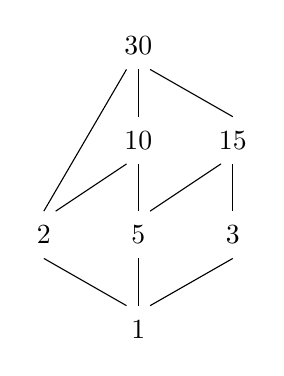
\begin{tikzpicture}[scale=0.6] %Replaced figure with tikz figure - TWJ 8/22/2010

\draw (0,0.5) -- (0,1.5);
\draw (0,2.5) -- (0,3.5);
\draw (2,2.5) -- (2,3.5);
\draw (0,4.5) -- (0,5.5);

\draw (0.25,5.5) -- (2,4.5);
\draw (-0.25,5.5) -- (-2,2.5);

\draw (1.75,3.5) -- (0.25,2.5);
\draw (-0.25,3.5) -- (-1.75,2.5);

\draw (2,1.5) -- (0.25,0.5);
\draw (-2,1.5) -- (-0.25,0.5);

\node at (0,6) {30};
\node at (0,4) {10};
\node at (2,4) {15};
\node at (-2, 2) {2};
\node at (0, 2) {5};
\node at (2, 2) {3};
\node at (0, 0) {1};

\end{tikzpicture}
\end{center}
 
 
 
\item[5.] 
False.
 

 
\item[6.]
(a) $(a \vee b \vee a') \wedge a$.
\begin{center}  
\tikzpreface{solution_circuit_a}
\begin{tikzpicture}[scale=0.8,node distance=5mm, text height=1.5ex,text depth=.25ex] %Replaced figure with tikz figure - TWJ 8/22/2010

\draw  (0,0) -- (2.2,0) (2.8,0) -- (4.7,0)  (5.3,0) -- (6,0);
\draw  (1,0) -- (1,1) -- (2.2,1)  (2.8,1) -- (4,1) -- (4,0);
\draw  (1,0) -- (1,-1) -- (2.2,-1)  (2.8,-1) -- (4,-1) -- (4,0);

\node at (2.5,-1) {$a'$};
\node at (2.5,0) {$b$};
\node at (2.5,1) {$a$};
\node at (5,0) {$a$};



\end{tikzpicture}
\end{center}
 


(c) $a \vee (a \wedge b)$.
\begin{center}  

\tikzpreface{solution_circuit_c}
\begin{tikzpicture}[scale=0.8,node distance=5mm, text height=1.5ex,text depth=.25ex] %Replaced figure with tikz figure - TWJ 8/22/2010

\draw  (0,0) -- (1,0) (4,0) -- (5,0);
\draw  (1,0) -- (1,1) -- (1.7,1)  (2.3,1) -- (2.7,1)  (3.3,1) -- (4,1) -- (4,0);
\draw  (1,0) -- (1,-1) -- (2.2,-1)  (2.8,-1) -- (4,-1) -- (4,0);

\node at (2.5,-1) {$a$};
\node at (2,1) {$a$};
\node at (3,1) {$b$};



\end{tikzpicture}
\end{center}
 
 
 
 
\item[8.]
Not equivalent.
 
\item[10.]
$a' \wedge [(a \wedge b') \vee b] = a \wedge (a \vee b)$.

\item[15.]
Let $I, J$ be ideals in $R$. We need to show that $I + J 
= \{ r + s : r \in
I \mbox{ and } s \in J  \}$ is the smallest ideal in $R$ containing
both $I$ and $J$. If $r_1, r_2 \in I$ and $s_1, s_2 \in J$, then
$(r_1 + s_1) + (r_2 + s_2) = (r_1 + r_2) +(s_1 + s_2)$ is in $I + J$.
For $a \in R$, $a(r_1 + s_1) = ar_1 + as_1 \in I + J$; hence, $I + J$
is an ideal in $R$.


\item[19.]
(a) No.

\item[21.]
$( \Rightarrow)$. $a = b \Rightarrow (a \wedge b') \vee (a' \wedge b)
= (a \wedge a') \vee (a' \wedge a) = O \vee O = O$. \\
$( \Leftarrow)$. $( a \wedge b') \vee (	a' \wedge b) = O \Rightarrow
a \vee b = (a \vee a) \vee b = a \vee (a \vee b) = a \vee [I \wedge
(a \vee b)] = a \vee [(a \vee a') \wedge (a \vee b)] = [a \vee
(a \wedge b')] \vee [a \vee (a' \wedge b)] = a \vee [(a \wedge b') \vee
(a' \wedge b)] = a \vee 0 = a$.  A symmetric argument shows that $a
\vee b = b$.



 
\end{itemize}
}
 
\subsection*{Chapter 20. Vector Spaces}
 
{\small
\begin{itemize}
 
\item[3.] 
${\mathbb Q}(\sqrt{2}, \sqrt{3}\, )$ has basis $\{ 1, \sqrt{2}, \sqrt{3},
\sqrt{6}\, \}$  over ${\mathbb Q}$.
 
\item[5.]
$P_n$ has basis $\{ 1, x, x^2, \ldots, x^{n-1} \}$.
 
\item[7.]
(a) Subspace of dimension 2 with basis $\{(1, 0, -3), (0, 1,
2) \}$.\\
(d) Not a subspace.
 
\item[10.]
$0 =  \alpha 0 = \alpha(-v+v) = \alpha(-v) + \alpha v \Rightarrow 
-\alpha v = \alpha(-v)$.
 
\item[12.]
Let $v_0 = 0, v_1, \ldots, v_n \in V$ and $\alpha_0 \neq 0, \alpha_1,
\ldots, \alpha_n \in F$. Then $\alpha_0 v_0 + \cdots + \alpha_n v_n =
0$.
 
\item[15.]
(a)
Let $u, v \in \ker(T)$ and $\alpha \in F$.  Then
\[
\begin{array}{c}
T(u +v) = T(u) + T(v) = 0 \\
T(\alpha v) = \alpha T(v) = \alpha 0 = 0.
\end{array}
\]
Hence, $u + v, \alpha v \in \ker(T) \Rightarrow \ker(T)$ is 
a subspace of
$V$. \\
(c) 
$T(u) = T(v) \Leftrightarrow T(u-v) = T(u) - T(v) = 0
\Leftrightarrow u-v = 0 \Leftrightarrow u = v$.
 
 
\item[17.]
(a)
Let $u, u' \in U$ and $v, v' \in V$. Then
\[
\begin{array}{c}
(u + v) + (u' + v') = (u + u') + (v + v') \in U + V \\
\alpha(u + v) = \alpha u + \alpha v \in U + V.
\end{array}
\]
 
\end{itemize}
}
 
\subsection*{Chapter 21. Fields}
 
{\small
\begin{itemize}
 
\item[1.] 
(a) $x^4 -\frac{2}{3} x^2 - \frac{62}{9}$.
(c) $x^4 - 2 x^2 + 25$.
 
\item[2.] 
(a) $\{ 1, \sqrt{2}, \sqrt{3}, \sqrt{6}\, \}$.
(c) $\{ 1, i, \sqrt{2}, \sqrt{2}\, i \}$.
(e) $\{1, 2^{1/6}, 2^{1/3}, 2^{1/2}, 2^{2/3}, 2^{5/6}  \}$.
 
\item[3.]
(a) ${\mathbb Q}(\sqrt{3}, \sqrt{7}\, )$.
 

\item[5.]
Use the fact that the elements of ${\mathbb Z}_2[x]/ \langle x^3 + x +
1\rangle$ are 0, 1, $\alpha$, $1 + \alpha$, $\alpha^2$, $1 + \alpha^2$,
$\alpha + \alpha^2$, $1 + \alpha + \alpha^2$ and the fact that
$\alpha^3 + \alpha + 1 = 0$. 


\item[8.]
False.


\item[14.]
Suppose that $E$ is algebraic over $F$ and $K$ is
algebraic over $E$. Let $\alpha \in K$. It suffices to show that
$\alpha$ is algebraic over some finite extension of $F$. Since
$\alpha$ is algebraic over $E$, it must be the zero of some polynomial
$p(x) = \beta_0 + \beta_1 x + \cdots + \beta_n x^n$ in $E[x]$. Hence
$\alpha$ is algebraic over $F(\beta_0, \ldots, \beta_n)$.


\item[22.]
${\mathbb Q}( \sqrt{3}, \sqrt{7}\, ) \supset {\mathbb Q}( \sqrt{3} +\sqrt{7}\,
)$ since $\{ 1, \sqrt{3}, \sqrt{7}, \sqrt{21}\, \}$ is a basis for
${\mathbb Q}( \sqrt{3}, \sqrt{7}\, )$ over ${\mathbb Q}$. Since $[{\mathbb Q}(
\sqrt{3}, \sqrt{7}\, ) : {\mathbb Q}] = 4$, $[{\mathbb Q}( \sqrt{3}
+\sqrt{7}\, ) : {\mathbb Q}] = 2$ or 4. Since the degree of the minimal
polynomial of $\sqrt{3} +\sqrt{7}$ is 4, ${\mathbb Q}( \sqrt{3},
\sqrt{7}\, ) = {\mathbb Q}( \sqrt{3} +\sqrt{7}\, )$.


\item[27.]
Let $\beta \in F(\alpha)$ not in $F$. Then $\beta =
p(\alpha)/q(\alpha)$, where $p$ and $q$ are polynomials in $\alpha$
with $q(\alpha) \neq 0$ and coefficients in $F$. If $\beta$ is
algebraic over $F$, then there exists a polynomial $f(x) \in F[x]$
such that $f(\beta) = 0$. Let $f(x) = a_0 + a_1 x + \cdots + a_n x^n$.
Then  
\[
0 = f(\beta) = f\left( 
\frac{p(\alpha)}{q(\alpha)} \right)
= a_0 + a_1 \left( \frac{p(\alpha)}{q(\alpha)} \right)  + \cdots + a_n
\left( \frac{p(\alpha)}{q(\alpha)} \right)^n. 
\]
Now multiply both sides by $q(\alpha)^n$ to show that there is a
polynomial in $F[x]$ that has $\alpha$ as a zero.




\end{itemize}
}
 
\subsection*{Chapter 22. Finite Fields}
 
{\small
\begin{itemize}

\item[1.]
(a) 2.
(c) 2.
 
\item[4.] 
There are eight elements in ${\mathbb Z}_2(\alpha)$. Exhibit two more
zeros of $x^3 + x^2 + 1$ other than $\alpha$ in these eight elements. 
 
\item[5.] 
Find an irreducible polynomial $p(x)$ in ${\mathbb Z}_3[x]$ of degree
3 and show that ${\mathbb Z}_3[x]/ \langle p(x) \rangle$ has 27
elements. 

\item[7.]
(a) $x^5 -1 = (x+1)(x^4+x^3 + x^2 + x+ 1)$. \\
(c) $x^9 -1 = (x+1)( x^2 + x+ 1)(x^6+x^3+1)$.
 
\item[8.]
True.

\item[11.]
(a) Use the fact that $x^7 -1 = (x+1)( x^3 + x+ 1)(x^3+x^2+1)$.

\item[12.]
False.

\item[17.]
If $p(x) \in F[x]$, then $p(x) \in E[x]$.


\item[18.]
Since $\alpha$ is algebraic over $F$ of degree $n$, we can write any
element $\beta \in F(\alpha)$ uniquely as $\beta = a_0  + a_1 \alpha +
\cdots + a_{n-1} \alpha^{n-1}$ with $a_i \in F$. There are $q^n$
possible $n$-tuples $(a_0, a_1, \ldots, a_{n-1})$.


\item[24.]
Factor $x^{p-1} - 1$ over ${\mathbb Z}_p$.


\end{itemize}
}
 
\subsection*{Chapter 23. Galois Theory}
 
{\small
\begin{itemize}
 
\item[1.]
(a) ${\mathbb Z}_2$.
(c) ${\mathbb Z}_2 \times {\mathbb Z}_2 \times {\mathbb Z}_2$.
 
\item[2.]
(a) Separable.
(c) Not separable.
 
\item[3.]
$[{\rm GF}(729): {\rm GF}(9)] = [{\rm GF}(729): {\rm GF}(3)] /[{\rm
GF}(9): {\rm GF}(3)] = 6/2 = 3 \Rightarrow G({\rm GF}(729)/ {\rm
GF}(9)) \cong {\mathbb Z}_3$. A generator for $G({\rm GF}(729)/ {\rm
GF}(9))$ is $\sigma$, where $\sigma_{3^6}( \alpha) = \alpha^{3^6} =
\alpha^{729}$ for $\alpha \in {\rm GF}(729)$.

\item[4.]
(a) $S_5$.
(c) $S_3$.

\item[5.]
(a) ${\mathbb Q}(i)$.


\item[7.]
Let $E$ be the splitting field of a cubic polynomial in $F[x]$. Show that
\mbox{$[E:F]$} is less than or equal to 6 and is divisible by 3. Since $G(E/F)$ is a subgroup of
$S_3$ whose order is divisible by 3, conclude that this group must be 
isomorphic to ${\mathbb Z}_3$ or $S_3$.
 
\item[9.]
$G$ is a subgroup of $S_n$.

\item[16.]
True.

\item[20.]
(a) Clearly $\omega, \omega^2, \ldots, \omega^{p-1}$ are
distinct since $\omega \neq 1$ or 0. To show that $\omega^i$ is a zero
of $\Phi_p$, calculate $\Phi_p( \omega^i)$. \\
(b) The conjugates of $\omega$ are $\omega, \omega^2, \ldots,
\omega^{p-1}$. Define a map  $\phi_i: {\mathbb Q}(\omega)
\rightarrow {\mathbb Q}(\omega^i)$ by 
\[
\phi_i(a_0 + a_1 \omega +
\cdots + a_{p-2} \omega^{p-2}) = a_0 + a_1 \omega^i + \cdots + c_{p-2} 
(\omega^i)^{p-2},
\]
where $a_i \in {\mathbb Q}$. Prove that $\phi_i$ is an isomorphism of
fields. Show that $\phi_2$ 
generates $G({\mathbb Q}(\omega)/{\mathbb Q})$. \\ 
(c)
Show that $\{ \omega, \omega^2, \ldots, \omega^{p-1} \}$ is a basis
for ${\mathbb Q}( \omega )$ over ${\mathbb Q}$, and consider which linear
combinations of $\omega, \omega^2, \ldots, \omega^{p-1}$ are left
fixed by all elements of $G( {\mathbb Q}( \omega ) / {\mathbb Q})$.
 
 
 
\end{itemize}
}
 
 
 
 
\pagestyle{headings}
 
 
 
 

{\small%%%%(c)
%%%%(c)  This file is a portion of the source for the textbook
%%%%(c)
%%%%(c)    Abstract Algebra: Theory and Applications
%%%%(c)    Copyright 1997 by Thomas W. Judson
%%%%(c)
%%%%(c)  See the file COPYING.txt for copying conditions
%%%%(c)
%%%%(c)
\chapter*{GNU Free Documentation License}

\addcontentsline{toc}{chapter}{GNU Free Documentation License}
\pagestyle{myheadings}
\markboth{GFDL LICENSE}{GFDL LICENSE}

 \begin{center}

       Version 1.2, November 2002

%% RAB, 2010/07/21
%% Copyright symbol ("\copyright") causes trouble in xhtml/jsmath conversion
 Copyright 2000,2001,2002  Free Software Foundation, Inc.
 
 \bigskip
 
     51 Franklin St, Fifth Floor, Boston, MA  02110-1301  USA
  
 \bigskip
 
 Everyone is permitted to copy and distribute verbatim copies
 of this license document, but changing it is not allowed.
\end{center}


\begin{center}
\textbf{\large Preamble}
\end{center}

The purpose of this License is to make a manual, textbook, or other
functional and useful document ``free'' in the sense of freedom: to
assure everyone the effective freedom to copy and redistribute it,
with or without modifying it, either commercially or noncommercially.
Secondarily, this License preserves for the author and publisher a way
to get credit for their work, while not being considered responsible
for modifications made by others.

This License is a kind of ``copyleft'', which means that derivative
works of the document must themselves be free in the same sense.  It
complements the GNU General Public License, which is a copyleft
license designed for free software.

We have designed this License in order to use it for manuals for free
software, because free software needs free documentation: a free
program should come with manuals providing the same freedoms that the
software does.  But this License is not limited to software manuals;
it can be used for any textual work, regardless of subject matter or
whether it is published as a printed book.  We recommend this License
principally for works whose purpose is instruction or reference.

\section*{1.\ Applicability And Definitions}
% \begin{center}
% {\Large\bf 1. APPLICABILITY AND DEFINITIONS\par}
% \phantomsection
% \addcontentsline{toc}{section}{1. APPLICABILITY AND DEFINITIONS}
% \end{center}

This License applies to any manual or other work, in any medium, that
contains a notice placed by the copyright holder saying it can be
distributed under the terms of this License.  Such a notice grants a
world-wide, royalty-free license, unlimited in duration, to use that
work under the conditions stated herein.  The ``\textbf{Document}'', below,
refers to any such manual or work.  Any member of the public is a
licensee, and is addressed as ``\textbf{you}''.  You accept the license if you
copy, modify or distribute the work in a way requiring permission
under copyright law.

A ``\textbf{Modified Version}'' of the Document means any work containing the
Document or a portion of it, either copied verbatim, or with
modifications and/or translated into another language.

A ``\textbf{Secondary Section}'' is a named appendix or a front-matter section of
the Document that deals exclusively with the relationship of the
publishers or authors of the Document to the Document's overall subject
(or to related matters) and contains nothing that could fall directly
within that overall subject.  (Thus, if the Document is in part a
textbook of mathematics, a Secondary Section may not explain any
mathematics.)  The relationship could be a matter of historical
connection with the subject or with related matters, or of legal,
commercial, philosophical, ethical or political position regarding
them.

The ``\textbf{Invariant Sections}'' are certain Secondary Sections whose titles
are designated, as being those of Invariant Sections, in the notice
that says that the Document is released under this License.  If a
section does not fit the above definition of Secondary then it is not
allowed to be designated as Invariant.  The Document may contain zero
Invariant Sections.  If the Document does not identify any Invariant
Sections then there are none.

The ``\textbf{Cover Texts}'' are certain short passages of text that are listed,
as Front-Cover Texts or Back-Cover Texts, in the notice that says that
the Document is released under this License.  A Front-Cover Text may
be at most 5 words, and a Back-Cover Text may be at most 25 words.

A ``\textbf{Transparent}'' copy of the Document means a machine-readable copy,
represented in a format whose specification is available to the
general public, that is suitable for revising the document
straightforwardly with generic text editors or (for images composed of
pixels) generic paint programs or (for drawings) some widely available
drawing editor, and that is suitable for input to text formatters or
for automatic translation to a variety of formats suitable for input
to text formatters.  A copy made in an otherwise Transparent file
format whose markup, or absence of markup, has been arranged to thwart
or discourage subsequent modification by readers is not Transparent.
An image format is not Transparent if used for any substantial amount
of text.  A copy that is not ``Transparent'' is called ``\textbf{Opaque}''.

Examples of suitable formats for Transparent copies include plain
ASCII without markup, Texinfo input format, LaTeX input format, SGML
or XML using a publicly available DTD, and standard-conforming simple
HTML, PostScript or PDF designed for human modification.  Examples of
transparent image formats include PNG, XCF and JPG.  Opaque formats
include proprietary formats that can be read and edited only by
proprietary word processors, SGML or XML for which the DTD and/or
processing tools are not generally available, and the
machine-generated HTML, PostScript or PDF produced by some word
processors for output purposes only.

The ``\textbf{Title Page}'' means, for a printed book, the title page itself,
plus such following pages as are needed to hold, legibly, the material
this License requires to appear in the title page.  For works in
formats which do not have any title page as such, ``Title Page'' means
the text near the most prominent appearance of the work's title,
preceding the beginning of the body of the text.

A section ``\textbf{Entitled XYZ}'' means a named subunit of the Document whose
title either is precisely XYZ or contains XYZ in parentheses following
text that translates XYZ in another language.  (Here XYZ stands for a
specific section name mentioned below, such as ``\textbf{Acknowledgements}'',
``\textbf{Dedications}'', ``\textbf{Endorsements}'', or ``\textbf{History}''.)  
To ``\textbf{Preserve the Title}''
of such a section when you modify the Document means that it remains a
section ``Entitled XYZ'' according to this definition.

The Document may include Warranty Disclaimers next to the notice which
states that this License applies to the Document.  These Warranty
Disclaimers are considered to be included by reference in this
License, but only as regards disclaiming warranties: any other
implication that these Warranty Disclaimers may have is void and has
no effect on the meaning of this License.

\section*{2.\ Verbatim Copying}
% \begin{center}
% {\Large\bf 2. VERBATIM COPYING\par}
% %% \phantomsection
% \addcontentsline{toc}{section}{2. VERBATIM COPYING}
% \end{center}

You may copy and distribute the Document in any medium, either
commercially or noncommercially, provided that this License, the
copyright notices, and the license notice saying this License applies
to the Document are reproduced in all copies, and that you add no other
conditions whatsoever to those of this License.  You may not use
technical measures to obstruct or control the reading or further
copying of the copies you make or distribute.  However, you may accept
compensation in exchange for copies.  If you distribute a large enough
number of copies you must also follow the conditions in section~3.

You may also lend copies, under the same conditions stated above, and
you may publicly display copies.

\section*{3.\ Copying In Quantity}
% \begin{center}
% {\Large\bf 3. COPYING IN QUANTITY\par}
% %% \phantomsection
% \addcontentsline{toc}{section}{3. COPYING IN QUANTITY}
% \end{center}


If you publish printed copies (or copies in media that commonly have
printed covers) of the Document, numbering more than 100, and the
Document's license notice requires Cover Texts, you must enclose the
copies in covers that carry, clearly and legibly, all these Cover
Texts: Front-Cover Texts on the front cover, and Back-Cover Texts on
the back cover.  Both covers must also clearly and legibly identify
you as the publisher of these copies.  The front cover must present
the full title with all words of the title equally prominent and
visible.  You may add other material on the covers in addition.
Copying with changes limited to the covers, as long as they preserve
the title of the Document and satisfy these conditions, can be treated
as verbatim copying in other respects.

If the required texts for either cover are too voluminous to fit
legibly, you should put the first ones listed (as many as fit
reasonably) on the actual cover, and continue the rest onto adjacent
pages.

If you publish or distribute Opaque copies of the Document numbering
more than 100, you must either include a machine-readable Transparent
copy along with each Opaque copy, or state in or with each Opaque copy
a computer-network location from which the general network-using
public has access to download using public-standard network protocols
a complete Transparent copy of the Document, free of added material.
If you use the latter option, you must take reasonably prudent steps,
when you begin distribution of Opaque copies in quantity, to ensure
that this Transparent copy will remain thus accessible at the stated
location until at least one year after the last time you distribute an
Opaque copy (directly or through your agents or retailers) of that
edition to the public.

It is requested, but not required, that you contact the authors of the
Document well before redistributing any large number of copies, to give
them a chance to provide you with an updated version of the Document.

\section*{4.\ Modifications}
% \begin{center}
% {\Large\bf 4. MODIFICATIONS\par}
% %% \phantomsection
% \addcontentsline{toc}{section}{4. MODIFICATIONS}
% \end{center}

You may copy and distribute a Modified Version of the Document under
the conditions of sections 2 and 3 above, provided that you release
the Modified Version under precisely this License, with the Modified
Version filling the role of the Document, thus licensing distribution
and modification of the Modified Version to whoever possesses a copy
of it.  In addition, you must do these things in the Modified Version:

\begin{itemize}
\item[A.] 
   Use in the Title Page (and on the covers, if any) a title distinct
   from that of the Document, and from those of previous versions
   (which should, if there were any, be listed in the History section
   of the Document).  You may use the same title as a previous version
   if the original publisher of that version gives permission.
   
\item[B.]
   List on the Title Page, as authors, one or more persons or entities
   responsible for authorship of the modifications in the Modified
   Version, together with at least five of the principal authors of the
   Document (all of its principal authors, if it has fewer than five),
   unless they release you from this requirement.
   
\item[C.]
   State on the Title page the name of the publisher of the
   Modified Version, as the publisher.
   
\item[D.]
   Preserve all the copyright notices of the Document.
   
\item[E.]
   Add an appropriate copyright notice for your modifications
   adjacent to the other copyright notices.
   
\item[F.]
   Include, immediately after the copyright notices, a license notice
   giving the public permission to use the Modified Version under the
   terms of this License, in the form shown in the Addendum below.
   
\item[G.]
   Preserve in that license notice the full lists of Invariant Sections
   and required Cover Texts given in the Document's license notice.
   
\item[H.]
   Include an unaltered copy of this License.
   
\item[I.]
   Preserve the section Entitled ``History'', Preserve its Title, and add
   to it an item stating at least the title, year, new authors, and
   publisher of the Modified Version as given on the Title Page.  If
   there is no section Entitled ``History'' in the Document, create one
   stating the title, year, authors, and publisher of the Document as
   given on its Title Page, then add an item describing the Modified
   Version as stated in the previous sentence.
   
\item[J.]
   Preserve the network location, if any, given in the Document for
   public access to a Transparent copy of the Document, and likewise
   the network locations given in the Document for previous versions
   it was based on.  These may be placed in the ``History'' section.
   You may omit a network location for a work that was published at
   least four years before the Document itself, or if the original
   publisher of the version it refers to gives permission.
   
\item[K.]
   For any section Entitled ``Acknowledgements'' or ``Dedications'',
   Preserve the Title of the section, and preserve in the section all
   the substance and tone of each of the contributor acknowledgements
   and/or dedications given therein.
   
\item[L.]
   Preserve all the Invariant Sections of the Document,
   unaltered in their text and in their titles.  Section numbers
   or the equivalent are not considered part of the section titles.
   
\item[M.]
   Delete any section Entitled ``Endorsements''.  Such a section
   may not be included in the Modified Version.
   
\item[N.]
   Do not retitle any existing section to be Entitled ``Endorsements''
   or to conflict in title with any Invariant Section.
   
\item[O.]
   Preserve any Warranty Disclaimers.
\end{itemize}

If the Modified Version includes new front-matter sections or
appendices that qualify as Secondary Sections and contain no material
copied from the Document, you may at your option designate some or all
of these sections as invariant.  To do this, add their titles to the
list of Invariant Sections in the Modified Version's license notice.
These titles must be distinct from any other section titles.

You may add a section Entitled ``Endorsements'', provided it contains
nothing but endorsements of your Modified Version by various
parties--for example, statements of peer review or that the text has
been approved by an organization as the authoritative definition of a
standard.

You may add a passage of up to five words as a Front-Cover Text, and a
passage of up to 25 words as a Back-Cover Text, to the end of the list
of Cover Texts in the Modified Version.  Only one passage of
Front-Cover Text and one of Back-Cover Text may be added by (or
through arrangements made by) any one entity.  If the Document already
includes a cover text for the same cover, previously added by you or
by arrangement made by the same entity you are acting on behalf of,
you may not add another; but you may replace the old one, on explicit
permission from the previous publisher that added the old one.

The author(s) and publisher(s) of the Document do not by this License
give permission to use their names for publicity for or to assert or
imply endorsement of any Modified Version.

\section*{5.\ Combining Documents}
% \begin{center}
% {\Large\bf 5. COMBINING DOCUMENTS\par}
% %% \phantomsection
% \addcontentsline{toc}{section}{5. COMBINING DOCUMENTS}
% \end{center}


You may combine the Document with other documents released under this
License, under the terms defined in section~4 above for modified
versions, provided that you include in the combination all of the
Invariant Sections of all of the original documents, unmodified, and
list them all as Invariant Sections of your combined work in its
license notice, and that you preserve all their Warranty Disclaimers.

The combined work need only contain one copy of this License, and
multiple identical Invariant Sections may be replaced with a single
copy.  If there are multiple Invariant Sections with the same name but
different contents, make the title of each such section unique by
adding at the end of it, in parentheses, the name of the original
author or publisher of that section if known, or else a unique number.
Make the same adjustment to the section titles in the list of
Invariant Sections in the license notice of the combined work.

In the combination, you must combine any sections Entitled ``History''
in the various original documents, forming one section Entitled
``History''; likewise combine any sections Entitled ``Acknowledgements'',
and any sections Entitled ``Dedications''.  You must delete all sections
Entitled ``Endorsements''.

\section*{6.\ Collections Of Documents}
% \begin{center}
% {\Large\bf 6. COLLECTIONS OF DOCUMENTS\par}
% %% \phantomsection
% \addcontentsline{toc}{section}{6. COLLECTIONS OF DOCUMENTS}
% \end{center}

You may make a collection consisting of the Document and other documents
released under this License, and replace the individual copies of this
License in the various documents with a single copy that is included in
the collection, provided that you follow the rules of this License for
verbatim copying of each of the documents in all other respects.

You may extract a single document from such a collection, and distribute
it individually under this License, provided you insert a copy of this
License into the extracted document, and follow this License in all
other respects regarding verbatim copying of that document.

\section*{7.\ Aggregation With Independent Works}
% \begin{center}
% {\Large\bf 7. AGGREGATION WITH INDEPENDENT WORKS\par}
% %% \phantomsection
% \addcontentsline{toc}{section}{7. AGGREGATION WITH INDEPENDENT WORKS}
% \end{center}


A compilation of the Document or its derivatives with other separate
and independent documents or works, in or on a volume of a storage or
distribution medium, is called an ``aggregate'' if the copyright
resulting from the compilation is not used to limit the legal rights
of the compilation's users beyond what the individual works permit.
When the Document is included in an aggregate, this License does not
apply to the other works in the aggregate which are not themselves
derivative works of the Document.

If the Cover Text requirement of section~3 is applicable to these
copies of the Document, then if the Document is less than one half of
the entire aggregate, the Document's Cover Texts may be placed on
covers that bracket the Document within the aggregate, or the
electronic equivalent of covers if the Document is in electronic form.
Otherwise they must appear on printed covers that bracket the whole
aggregate.

\section*{8.\ Translation}
% \begin{center}
% {\Large\bf 8. TRANSLATION\par}
% %% \phantomsection
% \addcontentsline{toc}{section}{8. TRANSLATION}
% \end{center}


Translation is considered a kind of modification, so you may
distribute translations of the Document under the terms of section~4.
Replacing Invariant Sections with translations requires special
permission from their copyright holders, but you may include
translations of some or all Invariant Sections in addition to the
original versions of these Invariant Sections.  You may include a
translation of this License, and all the license notices in the
Document, and any Warranty Disclaimers, provided that you also include
the original English version of this License and the original versions
of those notices and disclaimers.  In case of a disagreement between
the translation and the original version of this License or a notice
or disclaimer, the original version will prevail.

If a section in the Document is Entitled ``Acknowledgements'',
``Dedications'', or ``History'', the requirement (section~4) to Preserve
its Title (section~1) will typically require changing the actual
title.

\section*{9.\ Termination}
% \begin{center}
% {\Large\bf 9. TERMINATION\par}
% %% \phantomsection
% \addcontentsline{toc}{section}{9. TERMINATION}
% \end{center}


You may not copy, modify, sublicense, or distribute the Document except
as expressly provided for under this License.  Any other attempt to
copy, modify, sublicense or distribute the Document is void, and will
automatically terminate your rights under this License.  However,
parties who have received copies, or rights, from you under this
License will not have their licenses terminated so long as such
parties remain in full compliance.

\section*{10.\ Future Revisions Of This License}
% \begin{center}
% {\Large\bf 10. FUTURE REVISIONS OF THIS LICENSE\par}
% %% \phantomsection
% \addcontentsline{toc}{section}{10. FUTURE REVISIONS OF THIS LICENSE}
% \end{center}


The Free Software Foundation may publish new, revised versions
of the GNU Free Documentation License from time to time.  Such new
versions will be similar in spirit to the present version, but may
differ in detail to address new problems or concerns.  See
http://www.gnu.org/copyleft/.

Each version of the License is given a distinguishing version number.
If the Document specifies that a particular numbered version of this
License ``or any later version'' applies to it, you have the option of
following the terms and conditions either of that specified version or
of any later version that has been published (not as a draft) by the
Free Software Foundation.  If the Document does not specify a version
number of this License, you may choose any version ever published (not
as a draft) by the Free Software Foundation.

\section*{Addendum: How to use this License for your documents}
% \begin{center}
% {\Large\bf ADDENDUM: How to use this License for your documents\par}
% %% \phantomsection
% \addcontentsline{toc}{section}{ADDENDUM: How to use this License for your documents}
% \end{center}

To use this License in a document you have written, include a copy of
the License in the document and put the following copyright and
license notices just after the title page:

%% RAB, 2010/07/21
%% Copyright symbol ("\copyright") causes trouble in xhtml/jsmath conversion
\bigskip
\begin{quote}
    Copyright  YEAR  YOUR NAME.
    Permission is granted to copy, distribute and/or modify this document
    under the terms of the GNU Free Documentation License, Version 1.2
    or any later version published by the Free Software Foundation;
    with no Invariant Sections, no Front-Cover Texts, and no Back-Cover Texts.
    A copy of the license is included in the section entitled ``GNU
    Free Documentation License''.
\end{quote}
\bigskip
    
If you have Invariant Sections, Front-Cover Texts and Back-Cover Texts,
replace the ``with \dots\ Texts.'' line with this:

\bigskip
\begin{quote}
    with the Invariant Sections being LIST THEIR TITLES, with the
    Front-Cover Texts being LIST, and with the Back-Cover Texts being LIST.
\end{quote}
\bigskip
    
If you have Invariant Sections without Cover Texts, or some other
combination of the three, merge those two alternatives to suit the
situation.

If your document contains nontrivial examples of program code, we
recommend releasing these examples in parallel under your choice of
free software license, such as the GNU General Public License,
to permit their use in free software.
}
%%%%(c)
%%%%(c)  This file is a portion of the source for the textbook
%%%%(c)
%%%%(c)    Abstract Algebra: Theory and Applications
%%%%(c)    Copyright 1997 by Thomas W. Judson
%%%%(c)
%%%%(c)  See the file COPYING.txt for copying conditions
%%%%(c)
%%%%(c)
\chapter*{Notation}

% Print versions need page headers, ToC entry
% tex4ht versions get their own ToC automatically
\ifthenelse{\boolean{basic}}{%
\phantomsection
\addcontentsline{toc}{chapter}{Notation}
\pagestyle{myheadings}
\markboth{NOTATION}{NOTATION}
}{}

The following table defines the  notation used in this book. Page numbers
refer to the first appearance of each symbol.
%
\begin{center}
\begin{longtable}{llr}
%
\multicolumn{1}{l}\textbf{Symbol} & \multicolumn{1}{l}\textbf{Description} & \multicolumn{1}{r}\textbf{Page} \\
&&\\
\endfirsthead
%
\multicolumn{1}{l}\textbf{Symbol} & \multicolumn{1}{l}\textbf{Description} & \multicolumn{1}{r}\textbf{Page} \\
&&\\
\endhead
%
$a \in A$ & $a$ is in the set $A$ & \pageref{sets_membership} \\
%
${\mathbb N}$ & the natural numbers & \pageref{naturalnum} \\
%
${\mathbb Z}$ & the integers & \pageref{sets_integers} \\
%
${\mathbb Q}$ & the rational numbers & \pageref{rationals} \\
%
${\mathbb R}$ & the real numbers & \pageref{reals} \\
%
${\mathbb C}$ & the complex numbers & \pageref{complexnum} \\
%
$A \subset B$ & $A$ is a subset of $B$ & \pageref{setcontain} \\
%
$\emptyset$ & the empty set & \pageref{theemptyset} \\
%
$A \cup B$ & union of sets $A$ and $B$ & \pageref{union} \\
%
$A \cap B$ & intersection of sets $A$ and $B$ & \pageref{intersection} \\
%
$A'$ & complement of the  set $A$ & \pageref{setcomplement} \\
%
$A \setminus B$ & difference between sets $A$ and $B$ & \pageref{setdifference} \\
%
$A \times B$ & Cartesian product of sets $A$ and $B$ & \pageref{cartesian} \\
%
$A^n$ & $A \times \cdots \times A$ ($n$ times) & \pageref{ncartesian} \\
%
$id$ & identity mapping & \pageref{noteidentity} \\
%
$f^{-1}$ & inverse of the function $f$	& \pageref{inversefunc} \\
%
$a \equiv b \pmod{n}$ & $a$ is congruent to $b$ modulo $n$ & \pageref{amodb} \\
%
$n!$ & $n$ factorial & \pageref{factorial} \\
%
$\left(\begin{array}{c}n \\ k \end{array} \right)$ & binomial coefficient $n!/(k! (n-k)!)$ & \pageref{binomial} \\
%
$m \mid n$ & $m$ divides $n$ & \pageref{divides} \\
%
$\gcd(m, n)$ & greatest common divisor of $m$ and $n$ & \pageref{greatestcd}\\
%
${\cal P}(X)$ & power set of $X$ & \pageref{powerset} \\
%
${\mathbb Z}_n$ & the integers modulo $n$ & \pageref{integersmodn} \\
%
$\lcm(m,n)$ & least common multiple of $m$ and $n$ & \pageref{leastcm} \\
%
$U(n)$ & group of units in ${\mathbb Z}_n$ & \pageref{groupofunits} \\
%
${\mathbb M}_n ( {\mathbb R})$ & the $n \times n$ matrices with entries in ${\mathbb R}$ &  \pageref{notematrices} \\
%
$\det A$ & determinant of $A$ & \pageref{determinant} \\
%
$GL_n({\mathbb R})$ & general linear group & \pageref{generallinear} \\
%
$Q_8$ & the group of quaternions & \pageref{notequateriongroup} \\
%
${\mathbb C}^\ast$ & the multiplicative group of complex numbers & \pageref{noteCstar} \\
%
$|G|$ & order of a group $G$ & \pageref{noteorder} \\
%
${\mathbb R}^*$ & the multiplicative group of real numbers & \pageref{noteRstar} \\
%
${\mathbb Q}^*$ & the multiplicative group of rational numbers & \pageref{noteQstar} \\
%
$SL_n({\mathbb R})$ & special linear group & \pageref{speciallinear} \\
%
$Z(G)$ & center of a group $G$ & \pageref{centerofagroup} \\
%
$\langle a \rangle$ & cyclic subgroup generated by $a$ & \pageref{generatedby} \\
%
$|a|$ & order of an element $a$ & \pageref{noteelementorder} \\
%
$\cis \theta$ & $\cos \theta + i \sin \theta$ & \pageref{cosisin} \\
%
${\mathbb T}$ & the circle group & \pageref{notecirclegroup} \\
%
$S_n$ & symmetric group on $n$ letters & \pageref{symmetricgroup} \\
%
$(a_1, a_2, \ldots, a_k )$ & cycle of length $k$ & \pageref{notecycle} \\
%
$A_n$ & alternating group on $n$ letters & \pageref{alternatinggroup} \\
%
$D_n$ & dihedral group & \pageref{dihedralgroup} \\
%
$[G:H]$ & index of a subgroup $H$ in a group $G$ & \pageref{indexofasubgroup}  \\
%
${\cal L}_H$ & set of left cosets of $H$ in a group $G$ & \pageref{notesetleft} \\
%
${\cal R}_H$ & set of right cosets of $H$ in a group $G$ & \pageref{notesetright}  \\
%
$d({\mathbf x}, {\mathbf y})$ & Hamming distance between ${\mathbf x}$ and ${\mathbf y}$ & \pageref{noteHammingdist} \\
%
$d_{\min}$ & minimum distance of a code & \pageref{notemindist}\\
%
$w({\mathbf x})$ & weight of ${\mathbf x}$ & \pageref{noteweight} \\
%
${\mathbb M}_{m \times n}({\mathbb Z}_2)$ & set of $m$ by $n$ matrices with entries in ${\mathbb Z}_2$ & \pageref{notembyn} \\
%
${\rm Null}(H)$ & null space of a matrix $H$ & \pageref{notenull} \\
%
$\delta_{ij}$ & Kronecker delta & \pageref{notekron} \\
%
$G \cong H$ & $G$ is isomorphic to $H$ & \pageref{noteisomorph} \\
%
$Aut(G)$ & automorphism group of $G$ & \pageref{noteauto} \\
%
$i_g$ & $i_g(x) = gxg^{-1}$ & \pageref{noteinner} \\
%
$Inn(G)$ & inner automorphism group of $G$ & \pageref{noteinneraut} \\
%
$\rho_g$ & right regular representation & \pageref{noterightreg} \\
%
$G/N$ & factor group of $G$ mod $N$ & \pageref{notefactor} \\
%
$\ker \phi$ & kernel of $\phi$ & \pageref{kernelofphi} \\
%
$G'$ & commutator subgroup of $G$ & \pageref{commutatorsubgroup} \\
%
$(a_{ij})$ & matrix & \pageref{matrixnote} \\
%
$O(n)$ & orthogonal group & \pageref{noteorthogonal} \\
%
$\| {\mathbf x} \|$ & length of a vector ${\mathbf x}$ & \pageref{notelengthvect} \\
%
$SO(n)$ & special orthogonal group & \pageref{notespecialorthog} \\
%
$E(n)$ & Euclidean group & \pageref{noteeuclidgroup} \\
%
${\cal O}_x$ & orbit of $x$ & \pageref{noteorbit} \\
%
$X_g$ & fixed point set of $g$ & \pageref{notefixed} \\
%
$G_x$ & isotropy subgroup of $x$ & \pageref{noteisotropy} \\
%
$X_G$ & set of fixed points in a $G$-set $X$ & \pageref{noteXG} \\
%
$N(H)$ & normalizer of a subgroup $H$ & \pageref{notenormalizer} \\
%
${\mathbb H}$ & the ring of quaternions & \pageref{noteringH} \\
%
\mbox{char$\, R$} & characteristic of a ring $R$ & \pageref{ringchar} \\
%
${\mathbb Z}[i ]$ & the Gaussian integers & \pageref{gaussianintegers} \\
%
${\mathbb Z}_{(p)}$ & ring of integers localized at $p$ & \pageref{notelocalint} \\
%
$R[x]$ & ring of polynomials over $R$ & \pageref{polynomialring} \\
%
$\deg p(x)$ & degree of $p(x)$ & \pageref{polydegree} \\
%
$R[x_1, x_2, \ldots, x_n]$ & ring of polynomials in $n$ variables & \pageref{notepolynvar} \\
%
$\phi_{\alpha}$ & evaluation homomorphism at $\alpha$ & \pageref{noteevalhomo} \\
%
${\mathbb Q}(x)$ & field of rational functions over ${\mathbb Q}$ & \pageref{noteratpoly} \\
%
$\nu(a)$ & Euclidean valuation of $a$ & \pageref{notevaluation} \\
%
$F(x)$ & field of rational functions in $x$ & \pageref{noteratfun} \\
%
$F(x_1, \ldots, x_n)$ & field of rational functions in $x_1, \ldots, x_n$ & \pageref{noteratnvar} \\
%
$a \preceq b$ &  $a$ is less than $b$ & \pageref{lessthan} \\
%
$a \wedge b$ & meet of $a$ and $b$ & \pageref{meet} \\
%
$a \vee b$ & join of $a$ and $b$ & \pageref{join} \\
%
$I$ & largest element in a lattice & \pageref{notelargeposet} \\
%
$O$ & smallest element in a lattice & \pageref{notesmallposet} \\
%
$a'$ & complement of $a$ in a lattice &\pageref{notedlatticecomp}  \\
%
$\dim V$ & dimension of a vector space $V$ & \pageref{vectdim} \\
%
$U \oplus V$ & direct sum of vector spaces $U$ and $V$ & \pageref{notedirectsum} \\
%
$\mbox{Hom}(V, W)$ & set of all linear transformations from $U$ to $V$ & \pageref{noteHom} \\
%
$V^\ast$ & dual of a vector space $V$ & \pageref{notedual} \\
%
$F( \alpha_1, \ldots, \alpha_n)$ & smallest field containing $F$ and $\alpha_1, \ldots, \alpha_n$ & \pageref{notefieldcont}\\
%
$[E:F]$ & dimension of a field extension of $E$ over $F$ & \pageref{notedegext} \\
%
GF$(p^n)$ & Galois field of order $p^n$ & \pageref{galoisfield} \\
%
$F^*$ & multiplicative group of a field $F$ & \pageref{ntmultgrp} \\
%
$G(E/F)$ & Galois group of $E$ over $F$ &\pageref{notegalois} \\
%
$F_{\{\sigma_i \}}$ & field fixed by automorphisms $\sigma_i$ & \pageref{noteFixedfield} \\
%
$F_G$ & field fixed by automorphism group $G$ & \pageref{noteFixedG} \\
%
$\Delta^2$ & discriminant of a polynomial & \pageref{discriminant}
%
\end{longtable}
\end{center}




{\small\printindex}
%
% RAB, 2009/01/28
% Ditched endnotes in favor of improved notation.tex
%
\end{document}
